%% The first command in your LaTeX source must be the \documentclass command.
\documentclass[sigconf,authorversion]{acmart}
\usepackage{pgf}
\usepackage{pgfplots}
%% NOTE that a single column version may be required for
%% submission and peer review. This can be done by changing
%% the \doucmentclass[...]{acmart} in this template to
%% \documentclass[manuscript,screen,review]{acmart}
\providecommand{\tightlist}{%
  \setlength{\itemsep}{0pt}\setlength{\parskip}{0pt}}

\begin{document}
\settopmatter{printacmref=false}
\setcopyright{none}
\renewcommand\footnotetextcopyrightpermission[1]{}
\pagestyle{plain}
\title{Modeling the Latent Space of Symbolic String Quartet Music}

%%
%% The "author" command and its associated commands are used to define
%% the authors and their affiliations.
%% Of note is the shared affiliation of the first two authors, and the
%% "authornote" and "authornotemark" commands
%% used to denote shared contribution to the research.

\author{Alex Kyllo}
\email{akyllo@uw.edu}
\affiliation{%
  \institution{University of Washington}
  \city{Bothell}
  \state{WA}
  \country{USA}
}

\begin{abstract}
  This paper presents the results of a project to apply a recurrent
  variational autoencoder to the task of modeling a latent space for
  generating pieces of multi-instrument symbolic classical music
  through interpolation.
\end{abstract}

\keywords{deep learning, recurrent neural networks, sequential models,
  music modeling, latent space modeling, generative modeling}

\maketitle

\section{Introduction}

Machine learning models of music have interesting applications in
music information retrieval and creative tools for musical artists and
educators. Generative models can create accompaniments for music,
blend and transfer styles between clips of music, and even generate
entirely new music. Music is challenging to model because it is
inherently high-dimensional, exhibiting a complex hierarchy of
recurring patterns and long-range temporal dependencies, and because
musical scores have multiple possible digital representations with
distinct advantages and disadvantages.

Depending on the task, machine learning models of music may be trained
on the audio signal of a musical performance, either in a time domain
or a frequency domain representation, or they may be trained on a
digital symbolic representation of music, the most common of which is
MIDI (Musical Instrument Digital Interface) notation. MIDI is an
encoding of music as streams of bytes in one or more tracks or
channels, each representing a sequence of 128 possible pitch values
(where 0 is the lowest pitch and 127 is the highest), along with
timing, pressure and instrument identifier values. A generative
symbolic music model can produce a symbolic score in MIDI format,
which must be played by synthesizer software or by humans to produce
an audio music performance. This project focuses on generative
modeling of symbolic (MIDI) music to compose original musical scores
by blending input scores through continuous latent space interpolation.

A survey of related works in generative modeling of polyphonic music
turned up several models focused on multi-instrument pop/rock music
arrangements or classical piano performances. In contrast, this
project focuses on variational autoencoding and latent space
interpolation of classical string quartets (arrangements for an
ensemble of two violins, one viola and one cello) and is, to the
author's knowledge, the first project to apply this modeling approach
to this type of musical arrangement.

\section{Related Work}

The state of the art in music generation still has a long way to go
before it can consistently generate music scores or performances that
would be enjoyable and popular for humans to listen to, but for this
reason it is an area of significant opportunity, where a number of
recent research projects have shown promising progress.

Google's \href{https://magenta.tensorflow.org/}{Magenta} is an
umbrella project for music deep learning research and development of
software tools to expose these models for use by creative artists and
students.

MusicVAE, part of the Magenta project, is a variational Long
Short-Term Memory (LSTM) autoencoder for MIDI that incorporates a
novel hierarchical structure using a ``conductor'' recurrent layer in
its decoder model to better capture structure at multiple levels and
avoid the problem of ``posterior/mode collapse'' whereby a generative
model learns to ignore its latent codes and rely on autoregression to
generate output sequences \cite{roberts_hierarchical_2018}. This model
is trained on 16-bar paragraphs of music and is capable of generating
new melodies that blend two given melodies together via latent space
interpolation. Among the literature surveyed, MusicVAE's approach is
the most similar to this work; in comparison our model is
significantly simpler and works on a single bar of music at a time.

Another Magenta model called Music Transformer is a generative model
that borrows its approach from the Natural Language Processing (NLP)
domain, using a self-attention network to model MIDI music as a
sequence of discrete tokens with relative positional dependencies
\cite{huang_music_2018}. The focus of this model is on learning
long-term dependencies in music to produce longer clips of music with
coherent structure. Music Transformer was trained on a dataset of
Piano-e-competition performances \cite{hawthorne2019enabling} and its
generated piano music received favorable qualitative (Likert scale)
ratings from human listeners for its resemblance to human-composed
music \cite{huang_music_2018}. In contrast to MusicVAE and this work,
Music Transformer is capable of generating much longer sequences of
music, but does so via sequence extrapolation rather than
interpolation, so it can continue a given priming melody but does not
blend multiple given melodies together. It also assumes a single
instrument track (piano).

MuseGAN \cite{dong2017musegan} is an application of Generative
Adversarial Networks (GAN) to polyphonic MIDI music generation,
trained on four-bar phrases of a multi-track pianoroll representation
of rock songs from the Lakh Midi Dataset
\cite{raffel_learning-based_2016}. Like MusicVAE, MuseGAN includes a
two-level generator that first samples latent codes at the phrase or
bar level, then generates notes within the bars, to produce
longer-term structural patterns.

A major advantage of working with the symbolic representation of music
is that it is of far lower dimensionality than the raw audio waveforms
of a recorded performance, which makes it less computationally
expensive. However, there are many stylistic aspects of musical
performance that are not captured by a symbolic representation, and
may be specific to a particular performer, so the expressiveness of
symbolic generative models is limited in comparison
\cite{manzelli_conditioning_2018}.

Other research has focused on modeling raw audio waveforms directly. WaveNet is
a causal convolutional neural network for generating raw audio waveforms,
developed by Google DeepMind, which achieves state of the art performance in
generating natural sounding speech from text, but is also capable of generating
short, realistic snippets of audio music \cite{oord_wavenet_2016}.
Another model named SampleRNN generates raw audio waveforms using a three-tier
hierarchy of gated recurrent units (GRU) to model recurrent structure at
multiple temporal resolutions \cite{mehri_samplernn_2017}.

Prior work points out that the division between symbolic music notes
and music performances, is analogous to the division between symbolic
language and utterances in speech, which may inspire ideas for
combining the two approaches \cite{hawthorne2019enabling}. A paper
from Boston University describes an effort to combine the symbolic and
waveform approaches to music modeling, by training an LSTM to learn
melodic structure of different styles of music, then providing
generations from this model as conditioning inputs to a WaveNet-based
raw audio generator \cite{manzelli_conditioning_2018}.

While there may be significant opportunity in future approaches that
combining the two, contemporary research generally treats symbolic and
audio music modeling as separate problem domains and this work does
the same, choosing to focus on symbolic music.

\section{Methods}

\subsection{Datasets}

The dataset used for this research project is MusicNet, which is a
collection of 330 freely licensed European classical music recordings
with aligned MIDI scores \cite{thickstun2017learning}.  The model is
trained on 36 string quartets (four-part arrangements with two
violins, one viola and one cello) by composers Bach, Beethoven,
Dvorak, Haydn, Mozart, and Ravel.

\subsection{Data Preprocessing}

Several choices must be made in how to preprocess binary MIDI files
into training examples for a neural network. There are multiple
open-source Python packages that assist with the process of reading
MIDI files from their binary on-disk representations into Python
objects, such as pretty\_midi \cite{raffel_pretty_midi_2014},
Pypianoroll \cite{dong_pypianoroll_2018} and music21
\cite{cuthbert_music21_2010}.

In order to accommodate polyphonic music, we each MIDI file is
converted into a modified pianoroll representation, an example of
which is visualized in Figure \ref{pianoroll}. While the standard
pianoroll represents each time-step as a multi-hot encoded vector of
note values, because most notes are not being played at most timesteps
there is an extreme class imbalance and sparsity in the matrix. This
is reported in \cite{kumar2019polyphonic} to cause problems in model
fitting and metrics calculation, so they introduce an alternative
``multi-stream'' representation of the pianoroll, which we closely,
(but not exactly) emulate in this work.

In our modified representation, each instrument track is a sequence of
integers from 0-129 representing the MIDI note pitch value being
played at the given time step, where values 0-127 are pitches, 128 is
a rest (silence) and 129 is sustain, indicating that the previously
played pitch is held continuously. MIDI data contains pressure values
that indicate how hard or soft each note is played; this information
is discarded in our preprocessing and all notes are represented with
constant pressure. Because chords (multiple notes being played
simultaneously by the same instrument) are relatively rare in string
quartets, the lowest note of each chord is taken and the rest
discarded, to reduce dimensionality. Because notes at the extreme low
and high end are rare and are out of range of common instruments, the
note pitch values are clipped to a narrower range and ordinal
encoded. For the 36 string quartets found in the MusicNet database,
this results in 66 distinct values, where 0-63 represent notes played
by the violins, viola and cello, 64 is rest and 65 is sustain. Figure
\ref{pitch_dist} depicts the distribution of these pitch values per
instrument. Our software package also includes functions to convert
this representation back into a Music21 Score object, which can then
be written to a MIDI file.

\begin{figure}[htbp]
    \begin{center}
        \scalebox{0.6}{%% Creator: Matplotlib, PGF backend
%%
%% To include the figure in your LaTeX document, write
%%   \input{<filename>.pgf}
%%
%% Make sure the required packages are loaded in your preamble
%%   \usepackage{pgf}
%%
%% Figures using additional raster images can only be included by \input if
%% they are in the same directory as the main LaTeX file. For loading figures
%% from other directories you can use the `import` package
%%   \usepackage{import}
%%
%% and then include the figures with
%%   \import{<path to file>}{<filename>.pgf}
%%
%% Matplotlib used the following preamble
%%   \usepackage{fontspec}
%%   \setmainfont{DejaVuSerif.ttf}[Path=\detokenize{/home/alex/miniconda3/envs/musiclearn/lib/python3.9/site-packages/matplotlib/mpl-data/fonts/ttf/}]
%%   \setsansfont{DejaVuSans.ttf}[Path=\detokenize{/home/alex/miniconda3/envs/musiclearn/lib/python3.9/site-packages/matplotlib/mpl-data/fonts/ttf/}]
%%   \setmonofont{DejaVuSansMono.ttf}[Path=\detokenize{/home/alex/miniconda3/envs/musiclearn/lib/python3.9/site-packages/matplotlib/mpl-data/fonts/ttf/}]
%%
\begingroup%
\makeatletter%
\begin{pgfpicture}%
\pgfpathrectangle{\pgfpointorigin}{\pgfqpoint{6.000000in}{4.000000in}}%
\pgfusepath{use as bounding box, clip}%
\begin{pgfscope}%
\pgfsetbuttcap%
\pgfsetmiterjoin%
\pgfsetlinewidth{0.000000pt}%
\definecolor{currentstroke}{rgb}{1.000000,1.000000,1.000000}%
\pgfsetstrokecolor{currentstroke}%
\pgfsetstrokeopacity{0.000000}%
\pgfsetdash{}{0pt}%
\pgfpathmoveto{\pgfqpoint{0.000000in}{0.000000in}}%
\pgfpathlineto{\pgfqpoint{6.000000in}{0.000000in}}%
\pgfpathlineto{\pgfqpoint{6.000000in}{4.000000in}}%
\pgfpathlineto{\pgfqpoint{0.000000in}{4.000000in}}%
\pgfpathclose%
\pgfusepath{}%
\end{pgfscope}%
\begin{pgfscope}%
\pgfsetbuttcap%
\pgfsetmiterjoin%
\definecolor{currentfill}{rgb}{1.000000,1.000000,1.000000}%
\pgfsetfillcolor{currentfill}%
\pgfsetlinewidth{0.000000pt}%
\definecolor{currentstroke}{rgb}{0.000000,0.000000,0.000000}%
\pgfsetstrokecolor{currentstroke}%
\pgfsetstrokeopacity{0.000000}%
\pgfsetdash{}{0pt}%
\pgfpathmoveto{\pgfqpoint{0.750000in}{0.500000in}}%
\pgfpathlineto{\pgfqpoint{5.400000in}{0.500000in}}%
\pgfpathlineto{\pgfqpoint{5.400000in}{3.520000in}}%
\pgfpathlineto{\pgfqpoint{0.750000in}{3.520000in}}%
\pgfpathclose%
\pgfusepath{fill}%
\end{pgfscope}%
\begin{pgfscope}%
\pgfpathrectangle{\pgfqpoint{0.750000in}{0.500000in}}{\pgfqpoint{4.650000in}{3.020000in}}%
\pgfusepath{clip}%
\pgfsetbuttcap%
\pgfsetmiterjoin%
\definecolor{currentfill}{rgb}{0.839216,0.152941,0.156863}%
\pgfsetfillcolor{currentfill}%
\pgfsetfillopacity{0.750000}%
\pgfsetlinewidth{0.305505pt}%
\definecolor{currentstroke}{rgb}{0.000000,0.000000,0.000000}%
\pgfsetstrokecolor{currentstroke}%
\pgfsetdash{}{0pt}%
\pgfpathmoveto{\pgfqpoint{0.961364in}{0.500000in}}%
\pgfpathlineto{\pgfqpoint{1.003636in}{0.500000in}}%
\pgfpathlineto{\pgfqpoint{1.003636in}{1.047017in}}%
\pgfpathlineto{\pgfqpoint{0.961364in}{1.047017in}}%
\pgfpathclose%
\pgfusepath{stroke,fill}%
\end{pgfscope}%
\begin{pgfscope}%
\pgfpathrectangle{\pgfqpoint{0.750000in}{0.500000in}}{\pgfqpoint{4.650000in}{3.020000in}}%
\pgfusepath{clip}%
\pgfsetbuttcap%
\pgfsetmiterjoin%
\definecolor{currentfill}{rgb}{0.839216,0.152941,0.156863}%
\pgfsetfillcolor{currentfill}%
\pgfsetfillopacity{0.750000}%
\pgfsetlinewidth{0.305505pt}%
\definecolor{currentstroke}{rgb}{0.000000,0.000000,0.000000}%
\pgfsetstrokecolor{currentstroke}%
\pgfsetdash{}{0pt}%
\pgfpathmoveto{\pgfqpoint{1.003636in}{0.500000in}}%
\pgfpathlineto{\pgfqpoint{1.045909in}{0.500000in}}%
\pgfpathlineto{\pgfqpoint{1.045909in}{0.773509in}}%
\pgfpathlineto{\pgfqpoint{1.003636in}{0.773509in}}%
\pgfpathclose%
\pgfusepath{stroke,fill}%
\end{pgfscope}%
\begin{pgfscope}%
\pgfpathrectangle{\pgfqpoint{0.750000in}{0.500000in}}{\pgfqpoint{4.650000in}{3.020000in}}%
\pgfusepath{clip}%
\pgfsetbuttcap%
\pgfsetmiterjoin%
\definecolor{currentfill}{rgb}{0.839216,0.152941,0.156863}%
\pgfsetfillcolor{currentfill}%
\pgfsetfillopacity{0.750000}%
\pgfsetlinewidth{0.305505pt}%
\definecolor{currentstroke}{rgb}{0.000000,0.000000,0.000000}%
\pgfsetstrokecolor{currentstroke}%
\pgfsetdash{}{0pt}%
\pgfpathmoveto{\pgfqpoint{1.045909in}{0.500000in}}%
\pgfpathlineto{\pgfqpoint{1.088182in}{0.500000in}}%
\pgfpathlineto{\pgfqpoint{1.088182in}{0.500000in}}%
\pgfpathlineto{\pgfqpoint{1.045909in}{0.500000in}}%
\pgfpathclose%
\pgfusepath{stroke,fill}%
\end{pgfscope}%
\begin{pgfscope}%
\pgfpathrectangle{\pgfqpoint{0.750000in}{0.500000in}}{\pgfqpoint{4.650000in}{3.020000in}}%
\pgfusepath{clip}%
\pgfsetbuttcap%
\pgfsetmiterjoin%
\definecolor{currentfill}{rgb}{0.839216,0.152941,0.156863}%
\pgfsetfillcolor{currentfill}%
\pgfsetfillopacity{0.750000}%
\pgfsetlinewidth{0.305505pt}%
\definecolor{currentstroke}{rgb}{0.000000,0.000000,0.000000}%
\pgfsetstrokecolor{currentstroke}%
\pgfsetdash{}{0pt}%
\pgfpathmoveto{\pgfqpoint{1.088182in}{0.500000in}}%
\pgfpathlineto{\pgfqpoint{1.130455in}{0.500000in}}%
\pgfpathlineto{\pgfqpoint{1.130455in}{1.060548in}}%
\pgfpathlineto{\pgfqpoint{1.088182in}{1.060548in}}%
\pgfpathclose%
\pgfusepath{stroke,fill}%
\end{pgfscope}%
\begin{pgfscope}%
\pgfpathrectangle{\pgfqpoint{0.750000in}{0.500000in}}{\pgfqpoint{4.650000in}{3.020000in}}%
\pgfusepath{clip}%
\pgfsetbuttcap%
\pgfsetmiterjoin%
\definecolor{currentfill}{rgb}{0.839216,0.152941,0.156863}%
\pgfsetfillcolor{currentfill}%
\pgfsetfillopacity{0.750000}%
\pgfsetlinewidth{0.305505pt}%
\definecolor{currentstroke}{rgb}{0.000000,0.000000,0.000000}%
\pgfsetstrokecolor{currentstroke}%
\pgfsetdash{}{0pt}%
\pgfpathmoveto{\pgfqpoint{1.130455in}{0.500000in}}%
\pgfpathlineto{\pgfqpoint{1.172727in}{0.500000in}}%
\pgfpathlineto{\pgfqpoint{1.172727in}{0.943606in}}%
\pgfpathlineto{\pgfqpoint{1.130455in}{0.943606in}}%
\pgfpathclose%
\pgfusepath{stroke,fill}%
\end{pgfscope}%
\begin{pgfscope}%
\pgfpathrectangle{\pgfqpoint{0.750000in}{0.500000in}}{\pgfqpoint{4.650000in}{3.020000in}}%
\pgfusepath{clip}%
\pgfsetbuttcap%
\pgfsetmiterjoin%
\definecolor{currentfill}{rgb}{0.839216,0.152941,0.156863}%
\pgfsetfillcolor{currentfill}%
\pgfsetfillopacity{0.750000}%
\pgfsetlinewidth{0.305505pt}%
\definecolor{currentstroke}{rgb}{0.000000,0.000000,0.000000}%
\pgfsetstrokecolor{currentstroke}%
\pgfsetdash{}{0pt}%
\pgfpathmoveto{\pgfqpoint{1.172727in}{0.500000in}}%
\pgfpathlineto{\pgfqpoint{1.215000in}{0.500000in}}%
\pgfpathlineto{\pgfqpoint{1.215000in}{0.500000in}}%
\pgfpathlineto{\pgfqpoint{1.172727in}{0.500000in}}%
\pgfpathclose%
\pgfusepath{stroke,fill}%
\end{pgfscope}%
\begin{pgfscope}%
\pgfpathrectangle{\pgfqpoint{0.750000in}{0.500000in}}{\pgfqpoint{4.650000in}{3.020000in}}%
\pgfusepath{clip}%
\pgfsetbuttcap%
\pgfsetmiterjoin%
\definecolor{currentfill}{rgb}{0.839216,0.152941,0.156863}%
\pgfsetfillcolor{currentfill}%
\pgfsetfillopacity{0.750000}%
\pgfsetlinewidth{0.305505pt}%
\definecolor{currentstroke}{rgb}{0.000000,0.000000,0.000000}%
\pgfsetstrokecolor{currentstroke}%
\pgfsetdash{}{0pt}%
\pgfpathmoveto{\pgfqpoint{1.215000in}{0.500000in}}%
\pgfpathlineto{\pgfqpoint{1.257273in}{0.500000in}}%
\pgfpathlineto{\pgfqpoint{1.257273in}{1.221947in}}%
\pgfpathlineto{\pgfqpoint{1.215000in}{1.221947in}}%
\pgfpathclose%
\pgfusepath{stroke,fill}%
\end{pgfscope}%
\begin{pgfscope}%
\pgfpathrectangle{\pgfqpoint{0.750000in}{0.500000in}}{\pgfqpoint{4.650000in}{3.020000in}}%
\pgfusepath{clip}%
\pgfsetbuttcap%
\pgfsetmiterjoin%
\definecolor{currentfill}{rgb}{0.839216,0.152941,0.156863}%
\pgfsetfillcolor{currentfill}%
\pgfsetfillopacity{0.750000}%
\pgfsetlinewidth{0.305505pt}%
\definecolor{currentstroke}{rgb}{0.000000,0.000000,0.000000}%
\pgfsetstrokecolor{currentstroke}%
\pgfsetdash{}{0pt}%
\pgfpathmoveto{\pgfqpoint{1.257273in}{0.500000in}}%
\pgfpathlineto{\pgfqpoint{1.299545in}{0.500000in}}%
\pgfpathlineto{\pgfqpoint{1.299545in}{1.604666in}}%
\pgfpathlineto{\pgfqpoint{1.257273in}{1.604666in}}%
\pgfpathclose%
\pgfusepath{stroke,fill}%
\end{pgfscope}%
\begin{pgfscope}%
\pgfpathrectangle{\pgfqpoint{0.750000in}{0.500000in}}{\pgfqpoint{4.650000in}{3.020000in}}%
\pgfusepath{clip}%
\pgfsetbuttcap%
\pgfsetmiterjoin%
\definecolor{currentfill}{rgb}{0.839216,0.152941,0.156863}%
\pgfsetfillcolor{currentfill}%
\pgfsetfillopacity{0.750000}%
\pgfsetlinewidth{0.305505pt}%
\definecolor{currentstroke}{rgb}{0.000000,0.000000,0.000000}%
\pgfsetstrokecolor{currentstroke}%
\pgfsetdash{}{0pt}%
\pgfpathmoveto{\pgfqpoint{1.299545in}{0.500000in}}%
\pgfpathlineto{\pgfqpoint{1.341818in}{0.500000in}}%
\pgfpathlineto{\pgfqpoint{1.341818in}{0.500000in}}%
\pgfpathlineto{\pgfqpoint{1.299545in}{0.500000in}}%
\pgfpathclose%
\pgfusepath{stroke,fill}%
\end{pgfscope}%
\begin{pgfscope}%
\pgfpathrectangle{\pgfqpoint{0.750000in}{0.500000in}}{\pgfqpoint{4.650000in}{3.020000in}}%
\pgfusepath{clip}%
\pgfsetbuttcap%
\pgfsetmiterjoin%
\definecolor{currentfill}{rgb}{0.839216,0.152941,0.156863}%
\pgfsetfillcolor{currentfill}%
\pgfsetfillopacity{0.750000}%
\pgfsetlinewidth{0.305505pt}%
\definecolor{currentstroke}{rgb}{0.000000,0.000000,0.000000}%
\pgfsetstrokecolor{currentstroke}%
\pgfsetdash{}{0pt}%
\pgfpathmoveto{\pgfqpoint{1.341818in}{0.500000in}}%
\pgfpathlineto{\pgfqpoint{1.384091in}{0.500000in}}%
\pgfpathlineto{\pgfqpoint{1.384091in}{1.007392in}}%
\pgfpathlineto{\pgfqpoint{1.341818in}{1.007392in}}%
\pgfpathclose%
\pgfusepath{stroke,fill}%
\end{pgfscope}%
\begin{pgfscope}%
\pgfpathrectangle{\pgfqpoint{0.750000in}{0.500000in}}{\pgfqpoint{4.650000in}{3.020000in}}%
\pgfusepath{clip}%
\pgfsetbuttcap%
\pgfsetmiterjoin%
\definecolor{currentfill}{rgb}{0.839216,0.152941,0.156863}%
\pgfsetfillcolor{currentfill}%
\pgfsetfillopacity{0.750000}%
\pgfsetlinewidth{0.305505pt}%
\definecolor{currentstroke}{rgb}{0.000000,0.000000,0.000000}%
\pgfsetstrokecolor{currentstroke}%
\pgfsetdash{}{0pt}%
\pgfpathmoveto{\pgfqpoint{1.384091in}{0.500000in}}%
\pgfpathlineto{\pgfqpoint{1.426364in}{0.500000in}}%
\pgfpathlineto{\pgfqpoint{1.426364in}{0.500000in}}%
\pgfpathlineto{\pgfqpoint{1.384091in}{0.500000in}}%
\pgfpathclose%
\pgfusepath{stroke,fill}%
\end{pgfscope}%
\begin{pgfscope}%
\pgfpathrectangle{\pgfqpoint{0.750000in}{0.500000in}}{\pgfqpoint{4.650000in}{3.020000in}}%
\pgfusepath{clip}%
\pgfsetbuttcap%
\pgfsetmiterjoin%
\definecolor{currentfill}{rgb}{0.839216,0.152941,0.156863}%
\pgfsetfillcolor{currentfill}%
\pgfsetfillopacity{0.750000}%
\pgfsetlinewidth{0.305505pt}%
\definecolor{currentstroke}{rgb}{0.000000,0.000000,0.000000}%
\pgfsetstrokecolor{currentstroke}%
\pgfsetdash{}{0pt}%
\pgfpathmoveto{\pgfqpoint{1.426364in}{0.500000in}}%
\pgfpathlineto{\pgfqpoint{1.468636in}{0.500000in}}%
\pgfpathlineto{\pgfqpoint{1.468636in}{2.108193in}}%
\pgfpathlineto{\pgfqpoint{1.426364in}{2.108193in}}%
\pgfpathclose%
\pgfusepath{stroke,fill}%
\end{pgfscope}%
\begin{pgfscope}%
\pgfpathrectangle{\pgfqpoint{0.750000in}{0.500000in}}{\pgfqpoint{4.650000in}{3.020000in}}%
\pgfusepath{clip}%
\pgfsetbuttcap%
\pgfsetmiterjoin%
\definecolor{currentfill}{rgb}{0.839216,0.152941,0.156863}%
\pgfsetfillcolor{currentfill}%
\pgfsetfillopacity{0.750000}%
\pgfsetlinewidth{0.305505pt}%
\definecolor{currentstroke}{rgb}{0.000000,0.000000,0.000000}%
\pgfsetstrokecolor{currentstroke}%
\pgfsetdash{}{0pt}%
\pgfpathmoveto{\pgfqpoint{1.468636in}{0.500000in}}%
\pgfpathlineto{\pgfqpoint{1.510909in}{0.500000in}}%
\pgfpathlineto{\pgfqpoint{1.510909in}{1.099206in}}%
\pgfpathlineto{\pgfqpoint{1.468636in}{1.099206in}}%
\pgfpathclose%
\pgfusepath{stroke,fill}%
\end{pgfscope}%
\begin{pgfscope}%
\pgfpathrectangle{\pgfqpoint{0.750000in}{0.500000in}}{\pgfqpoint{4.650000in}{3.020000in}}%
\pgfusepath{clip}%
\pgfsetbuttcap%
\pgfsetmiterjoin%
\definecolor{currentfill}{rgb}{0.839216,0.152941,0.156863}%
\pgfsetfillcolor{currentfill}%
\pgfsetfillopacity{0.750000}%
\pgfsetlinewidth{0.305505pt}%
\definecolor{currentstroke}{rgb}{0.000000,0.000000,0.000000}%
\pgfsetstrokecolor{currentstroke}%
\pgfsetdash{}{0pt}%
\pgfpathmoveto{\pgfqpoint{1.510909in}{0.500000in}}%
\pgfpathlineto{\pgfqpoint{1.553182in}{0.500000in}}%
\pgfpathlineto{\pgfqpoint{1.553182in}{0.500000in}}%
\pgfpathlineto{\pgfqpoint{1.510909in}{0.500000in}}%
\pgfpathclose%
\pgfusepath{stroke,fill}%
\end{pgfscope}%
\begin{pgfscope}%
\pgfpathrectangle{\pgfqpoint{0.750000in}{0.500000in}}{\pgfqpoint{4.650000in}{3.020000in}}%
\pgfusepath{clip}%
\pgfsetbuttcap%
\pgfsetmiterjoin%
\definecolor{currentfill}{rgb}{0.839216,0.152941,0.156863}%
\pgfsetfillcolor{currentfill}%
\pgfsetfillopacity{0.750000}%
\pgfsetlinewidth{0.305505pt}%
\definecolor{currentstroke}{rgb}{0.000000,0.000000,0.000000}%
\pgfsetstrokecolor{currentstroke}%
\pgfsetdash{}{0pt}%
\pgfpathmoveto{\pgfqpoint{1.553182in}{0.500000in}}%
\pgfpathlineto{\pgfqpoint{1.595455in}{0.500000in}}%
\pgfpathlineto{\pgfqpoint{1.595455in}{1.778629in}}%
\pgfpathlineto{\pgfqpoint{1.553182in}{1.778629in}}%
\pgfpathclose%
\pgfusepath{stroke,fill}%
\end{pgfscope}%
\begin{pgfscope}%
\pgfpathrectangle{\pgfqpoint{0.750000in}{0.500000in}}{\pgfqpoint{4.650000in}{3.020000in}}%
\pgfusepath{clip}%
\pgfsetbuttcap%
\pgfsetmiterjoin%
\definecolor{currentfill}{rgb}{0.839216,0.152941,0.156863}%
\pgfsetfillcolor{currentfill}%
\pgfsetfillopacity{0.750000}%
\pgfsetlinewidth{0.305505pt}%
\definecolor{currentstroke}{rgb}{0.000000,0.000000,0.000000}%
\pgfsetstrokecolor{currentstroke}%
\pgfsetdash{}{0pt}%
\pgfpathmoveto{\pgfqpoint{1.595455in}{0.500000in}}%
\pgfpathlineto{\pgfqpoint{1.637727in}{0.500000in}}%
\pgfpathlineto{\pgfqpoint{1.637727in}{1.463562in}}%
\pgfpathlineto{\pgfqpoint{1.595455in}{1.463562in}}%
\pgfpathclose%
\pgfusepath{stroke,fill}%
\end{pgfscope}%
\begin{pgfscope}%
\pgfpathrectangle{\pgfqpoint{0.750000in}{0.500000in}}{\pgfqpoint{4.650000in}{3.020000in}}%
\pgfusepath{clip}%
\pgfsetbuttcap%
\pgfsetmiterjoin%
\definecolor{currentfill}{rgb}{0.839216,0.152941,0.156863}%
\pgfsetfillcolor{currentfill}%
\pgfsetfillopacity{0.750000}%
\pgfsetlinewidth{0.305505pt}%
\definecolor{currentstroke}{rgb}{0.000000,0.000000,0.000000}%
\pgfsetstrokecolor{currentstroke}%
\pgfsetdash{}{0pt}%
\pgfpathmoveto{\pgfqpoint{1.637727in}{0.500000in}}%
\pgfpathlineto{\pgfqpoint{1.680000in}{0.500000in}}%
\pgfpathlineto{\pgfqpoint{1.680000in}{0.500000in}}%
\pgfpathlineto{\pgfqpoint{1.637727in}{0.500000in}}%
\pgfpathclose%
\pgfusepath{stroke,fill}%
\end{pgfscope}%
\begin{pgfscope}%
\pgfpathrectangle{\pgfqpoint{0.750000in}{0.500000in}}{\pgfqpoint{4.650000in}{3.020000in}}%
\pgfusepath{clip}%
\pgfsetbuttcap%
\pgfsetmiterjoin%
\definecolor{currentfill}{rgb}{0.839216,0.152941,0.156863}%
\pgfsetfillcolor{currentfill}%
\pgfsetfillopacity{0.750000}%
\pgfsetlinewidth{0.305505pt}%
\definecolor{currentstroke}{rgb}{0.000000,0.000000,0.000000}%
\pgfsetstrokecolor{currentstroke}%
\pgfsetdash{}{0pt}%
\pgfpathmoveto{\pgfqpoint{1.680000in}{0.500000in}}%
\pgfpathlineto{\pgfqpoint{1.722273in}{0.500000in}}%
\pgfpathlineto{\pgfqpoint{1.722273in}{1.841449in}}%
\pgfpathlineto{\pgfqpoint{1.680000in}{1.841449in}}%
\pgfpathclose%
\pgfusepath{stroke,fill}%
\end{pgfscope}%
\begin{pgfscope}%
\pgfpathrectangle{\pgfqpoint{0.750000in}{0.500000in}}{\pgfqpoint{4.650000in}{3.020000in}}%
\pgfusepath{clip}%
\pgfsetbuttcap%
\pgfsetmiterjoin%
\definecolor{currentfill}{rgb}{0.839216,0.152941,0.156863}%
\pgfsetfillcolor{currentfill}%
\pgfsetfillopacity{0.750000}%
\pgfsetlinewidth{0.305505pt}%
\definecolor{currentstroke}{rgb}{0.000000,0.000000,0.000000}%
\pgfsetstrokecolor{currentstroke}%
\pgfsetdash{}{0pt}%
\pgfpathmoveto{\pgfqpoint{1.722273in}{0.500000in}}%
\pgfpathlineto{\pgfqpoint{1.764545in}{0.500000in}}%
\pgfpathlineto{\pgfqpoint{1.764545in}{0.500000in}}%
\pgfpathlineto{\pgfqpoint{1.722273in}{0.500000in}}%
\pgfpathclose%
\pgfusepath{stroke,fill}%
\end{pgfscope}%
\begin{pgfscope}%
\pgfpathrectangle{\pgfqpoint{0.750000in}{0.500000in}}{\pgfqpoint{4.650000in}{3.020000in}}%
\pgfusepath{clip}%
\pgfsetbuttcap%
\pgfsetmiterjoin%
\definecolor{currentfill}{rgb}{0.839216,0.152941,0.156863}%
\pgfsetfillcolor{currentfill}%
\pgfsetfillopacity{0.750000}%
\pgfsetlinewidth{0.305505pt}%
\definecolor{currentstroke}{rgb}{0.000000,0.000000,0.000000}%
\pgfsetstrokecolor{currentstroke}%
\pgfsetdash{}{0pt}%
\pgfpathmoveto{\pgfqpoint{1.764545in}{0.500000in}}%
\pgfpathlineto{\pgfqpoint{1.806818in}{0.500000in}}%
\pgfpathlineto{\pgfqpoint{1.806818in}{2.501542in}}%
\pgfpathlineto{\pgfqpoint{1.764545in}{2.501542in}}%
\pgfpathclose%
\pgfusepath{stroke,fill}%
\end{pgfscope}%
\begin{pgfscope}%
\pgfpathrectangle{\pgfqpoint{0.750000in}{0.500000in}}{\pgfqpoint{4.650000in}{3.020000in}}%
\pgfusepath{clip}%
\pgfsetbuttcap%
\pgfsetmiterjoin%
\definecolor{currentfill}{rgb}{0.839216,0.152941,0.156863}%
\pgfsetfillcolor{currentfill}%
\pgfsetfillopacity{0.750000}%
\pgfsetlinewidth{0.305505pt}%
\definecolor{currentstroke}{rgb}{0.000000,0.000000,0.000000}%
\pgfsetstrokecolor{currentstroke}%
\pgfsetdash{}{0pt}%
\pgfpathmoveto{\pgfqpoint{1.806818in}{0.500000in}}%
\pgfpathlineto{\pgfqpoint{1.849091in}{0.500000in}}%
\pgfpathlineto{\pgfqpoint{1.849091in}{1.240310in}}%
\pgfpathlineto{\pgfqpoint{1.806818in}{1.240310in}}%
\pgfpathclose%
\pgfusepath{stroke,fill}%
\end{pgfscope}%
\begin{pgfscope}%
\pgfpathrectangle{\pgfqpoint{0.750000in}{0.500000in}}{\pgfqpoint{4.650000in}{3.020000in}}%
\pgfusepath{clip}%
\pgfsetbuttcap%
\pgfsetmiterjoin%
\definecolor{currentfill}{rgb}{0.839216,0.152941,0.156863}%
\pgfsetfillcolor{currentfill}%
\pgfsetfillopacity{0.750000}%
\pgfsetlinewidth{0.305505pt}%
\definecolor{currentstroke}{rgb}{0.000000,0.000000,0.000000}%
\pgfsetstrokecolor{currentstroke}%
\pgfsetdash{}{0pt}%
\pgfpathmoveto{\pgfqpoint{1.849091in}{0.500000in}}%
\pgfpathlineto{\pgfqpoint{1.891364in}{0.500000in}}%
\pgfpathlineto{\pgfqpoint{1.891364in}{0.500000in}}%
\pgfpathlineto{\pgfqpoint{1.849091in}{0.500000in}}%
\pgfpathclose%
\pgfusepath{stroke,fill}%
\end{pgfscope}%
\begin{pgfscope}%
\pgfpathrectangle{\pgfqpoint{0.750000in}{0.500000in}}{\pgfqpoint{4.650000in}{3.020000in}}%
\pgfusepath{clip}%
\pgfsetbuttcap%
\pgfsetmiterjoin%
\definecolor{currentfill}{rgb}{0.839216,0.152941,0.156863}%
\pgfsetfillcolor{currentfill}%
\pgfsetfillopacity{0.750000}%
\pgfsetlinewidth{0.305505pt}%
\definecolor{currentstroke}{rgb}{0.000000,0.000000,0.000000}%
\pgfsetstrokecolor{currentstroke}%
\pgfsetdash{}{0pt}%
\pgfpathmoveto{\pgfqpoint{1.891364in}{0.500000in}}%
\pgfpathlineto{\pgfqpoint{1.933636in}{0.500000in}}%
\pgfpathlineto{\pgfqpoint{1.933636in}{2.012513in}}%
\pgfpathlineto{\pgfqpoint{1.891364in}{2.012513in}}%
\pgfpathclose%
\pgfusepath{stroke,fill}%
\end{pgfscope}%
\begin{pgfscope}%
\pgfpathrectangle{\pgfqpoint{0.750000in}{0.500000in}}{\pgfqpoint{4.650000in}{3.020000in}}%
\pgfusepath{clip}%
\pgfsetbuttcap%
\pgfsetmiterjoin%
\definecolor{currentfill}{rgb}{0.839216,0.152941,0.156863}%
\pgfsetfillcolor{currentfill}%
\pgfsetfillopacity{0.750000}%
\pgfsetlinewidth{0.305505pt}%
\definecolor{currentstroke}{rgb}{0.000000,0.000000,0.000000}%
\pgfsetstrokecolor{currentstroke}%
\pgfsetdash{}{0pt}%
\pgfpathmoveto{\pgfqpoint{1.933636in}{0.500000in}}%
\pgfpathlineto{\pgfqpoint{1.975909in}{0.500000in}}%
\pgfpathlineto{\pgfqpoint{1.975909in}{1.105005in}}%
\pgfpathlineto{\pgfqpoint{1.933636in}{1.105005in}}%
\pgfpathclose%
\pgfusepath{stroke,fill}%
\end{pgfscope}%
\begin{pgfscope}%
\pgfpathrectangle{\pgfqpoint{0.750000in}{0.500000in}}{\pgfqpoint{4.650000in}{3.020000in}}%
\pgfusepath{clip}%
\pgfsetbuttcap%
\pgfsetmiterjoin%
\definecolor{currentfill}{rgb}{0.839216,0.152941,0.156863}%
\pgfsetfillcolor{currentfill}%
\pgfsetfillopacity{0.750000}%
\pgfsetlinewidth{0.305505pt}%
\definecolor{currentstroke}{rgb}{0.000000,0.000000,0.000000}%
\pgfsetstrokecolor{currentstroke}%
\pgfsetdash{}{0pt}%
\pgfpathmoveto{\pgfqpoint{1.975909in}{0.500000in}}%
\pgfpathlineto{\pgfqpoint{2.018182in}{0.500000in}}%
\pgfpathlineto{\pgfqpoint{2.018182in}{0.500000in}}%
\pgfpathlineto{\pgfqpoint{1.975909in}{0.500000in}}%
\pgfpathclose%
\pgfusepath{stroke,fill}%
\end{pgfscope}%
\begin{pgfscope}%
\pgfpathrectangle{\pgfqpoint{0.750000in}{0.500000in}}{\pgfqpoint{4.650000in}{3.020000in}}%
\pgfusepath{clip}%
\pgfsetbuttcap%
\pgfsetmiterjoin%
\definecolor{currentfill}{rgb}{0.839216,0.152941,0.156863}%
\pgfsetfillcolor{currentfill}%
\pgfsetfillopacity{0.750000}%
\pgfsetlinewidth{0.305505pt}%
\definecolor{currentstroke}{rgb}{0.000000,0.000000,0.000000}%
\pgfsetstrokecolor{currentstroke}%
\pgfsetdash{}{0pt}%
\pgfpathmoveto{\pgfqpoint{2.018182in}{0.500000in}}%
\pgfpathlineto{\pgfqpoint{2.060455in}{0.500000in}}%
\pgfpathlineto{\pgfqpoint{2.060455in}{1.880108in}}%
\pgfpathlineto{\pgfqpoint{2.018182in}{1.880108in}}%
\pgfpathclose%
\pgfusepath{stroke,fill}%
\end{pgfscope}%
\begin{pgfscope}%
\pgfpathrectangle{\pgfqpoint{0.750000in}{0.500000in}}{\pgfqpoint{4.650000in}{3.020000in}}%
\pgfusepath{clip}%
\pgfsetbuttcap%
\pgfsetmiterjoin%
\definecolor{currentfill}{rgb}{0.839216,0.152941,0.156863}%
\pgfsetfillcolor{currentfill}%
\pgfsetfillopacity{0.750000}%
\pgfsetlinewidth{0.305505pt}%
\definecolor{currentstroke}{rgb}{0.000000,0.000000,0.000000}%
\pgfsetstrokecolor{currentstroke}%
\pgfsetdash{}{0pt}%
\pgfpathmoveto{\pgfqpoint{2.060455in}{0.500000in}}%
\pgfpathlineto{\pgfqpoint{2.102727in}{0.500000in}}%
\pgfpathlineto{\pgfqpoint{2.102727in}{1.576639in}}%
\pgfpathlineto{\pgfqpoint{2.060455in}{1.576639in}}%
\pgfpathclose%
\pgfusepath{stroke,fill}%
\end{pgfscope}%
\begin{pgfscope}%
\pgfpathrectangle{\pgfqpoint{0.750000in}{0.500000in}}{\pgfqpoint{4.650000in}{3.020000in}}%
\pgfusepath{clip}%
\pgfsetbuttcap%
\pgfsetmiterjoin%
\definecolor{currentfill}{rgb}{0.839216,0.152941,0.156863}%
\pgfsetfillcolor{currentfill}%
\pgfsetfillopacity{0.750000}%
\pgfsetlinewidth{0.305505pt}%
\definecolor{currentstroke}{rgb}{0.000000,0.000000,0.000000}%
\pgfsetstrokecolor{currentstroke}%
\pgfsetdash{}{0pt}%
\pgfpathmoveto{\pgfqpoint{2.102727in}{0.500000in}}%
\pgfpathlineto{\pgfqpoint{2.145000in}{0.500000in}}%
\pgfpathlineto{\pgfqpoint{2.145000in}{0.500000in}}%
\pgfpathlineto{\pgfqpoint{2.102727in}{0.500000in}}%
\pgfpathclose%
\pgfusepath{stroke,fill}%
\end{pgfscope}%
\begin{pgfscope}%
\pgfpathrectangle{\pgfqpoint{0.750000in}{0.500000in}}{\pgfqpoint{4.650000in}{3.020000in}}%
\pgfusepath{clip}%
\pgfsetbuttcap%
\pgfsetmiterjoin%
\definecolor{currentfill}{rgb}{0.839216,0.152941,0.156863}%
\pgfsetfillcolor{currentfill}%
\pgfsetfillopacity{0.750000}%
\pgfsetlinewidth{0.305505pt}%
\definecolor{currentstroke}{rgb}{0.000000,0.000000,0.000000}%
\pgfsetstrokecolor{currentstroke}%
\pgfsetdash{}{0pt}%
\pgfpathmoveto{\pgfqpoint{2.145000in}{0.500000in}}%
\pgfpathlineto{\pgfqpoint{2.187273in}{0.500000in}}%
\pgfpathlineto{\pgfqpoint{2.187273in}{1.214215in}}%
\pgfpathlineto{\pgfqpoint{2.145000in}{1.214215in}}%
\pgfpathclose%
\pgfusepath{stroke,fill}%
\end{pgfscope}%
\begin{pgfscope}%
\pgfpathrectangle{\pgfqpoint{0.750000in}{0.500000in}}{\pgfqpoint{4.650000in}{3.020000in}}%
\pgfusepath{clip}%
\pgfsetbuttcap%
\pgfsetmiterjoin%
\definecolor{currentfill}{rgb}{0.839216,0.152941,0.156863}%
\pgfsetfillcolor{currentfill}%
\pgfsetfillopacity{0.750000}%
\pgfsetlinewidth{0.305505pt}%
\definecolor{currentstroke}{rgb}{0.000000,0.000000,0.000000}%
\pgfsetstrokecolor{currentstroke}%
\pgfsetdash{}{0pt}%
\pgfpathmoveto{\pgfqpoint{2.187273in}{0.500000in}}%
\pgfpathlineto{\pgfqpoint{2.229545in}{0.500000in}}%
\pgfpathlineto{\pgfqpoint{2.229545in}{0.500000in}}%
\pgfpathlineto{\pgfqpoint{2.187273in}{0.500000in}}%
\pgfpathclose%
\pgfusepath{stroke,fill}%
\end{pgfscope}%
\begin{pgfscope}%
\pgfpathrectangle{\pgfqpoint{0.750000in}{0.500000in}}{\pgfqpoint{4.650000in}{3.020000in}}%
\pgfusepath{clip}%
\pgfsetbuttcap%
\pgfsetmiterjoin%
\definecolor{currentfill}{rgb}{0.839216,0.152941,0.156863}%
\pgfsetfillcolor{currentfill}%
\pgfsetfillopacity{0.750000}%
\pgfsetlinewidth{0.305505pt}%
\definecolor{currentstroke}{rgb}{0.000000,0.000000,0.000000}%
\pgfsetstrokecolor{currentstroke}%
\pgfsetdash{}{0pt}%
\pgfpathmoveto{\pgfqpoint{2.229545in}{0.500000in}}%
\pgfpathlineto{\pgfqpoint{2.271818in}{0.500000in}}%
\pgfpathlineto{\pgfqpoint{2.271818in}{2.021211in}}%
\pgfpathlineto{\pgfqpoint{2.229545in}{2.021211in}}%
\pgfpathclose%
\pgfusepath{stroke,fill}%
\end{pgfscope}%
\begin{pgfscope}%
\pgfpathrectangle{\pgfqpoint{0.750000in}{0.500000in}}{\pgfqpoint{4.650000in}{3.020000in}}%
\pgfusepath{clip}%
\pgfsetbuttcap%
\pgfsetmiterjoin%
\definecolor{currentfill}{rgb}{0.839216,0.152941,0.156863}%
\pgfsetfillcolor{currentfill}%
\pgfsetfillopacity{0.750000}%
\pgfsetlinewidth{0.305505pt}%
\definecolor{currentstroke}{rgb}{0.000000,0.000000,0.000000}%
\pgfsetstrokecolor{currentstroke}%
\pgfsetdash{}{0pt}%
\pgfpathmoveto{\pgfqpoint{2.271818in}{0.500000in}}%
\pgfpathlineto{\pgfqpoint{2.314091in}{0.500000in}}%
\pgfpathlineto{\pgfqpoint{2.314091in}{0.981298in}}%
\pgfpathlineto{\pgfqpoint{2.271818in}{0.981298in}}%
\pgfpathclose%
\pgfusepath{stroke,fill}%
\end{pgfscope}%
\begin{pgfscope}%
\pgfpathrectangle{\pgfqpoint{0.750000in}{0.500000in}}{\pgfqpoint{4.650000in}{3.020000in}}%
\pgfusepath{clip}%
\pgfsetbuttcap%
\pgfsetmiterjoin%
\definecolor{currentfill}{rgb}{0.839216,0.152941,0.156863}%
\pgfsetfillcolor{currentfill}%
\pgfsetfillopacity{0.750000}%
\pgfsetlinewidth{0.305505pt}%
\definecolor{currentstroke}{rgb}{0.000000,0.000000,0.000000}%
\pgfsetstrokecolor{currentstroke}%
\pgfsetdash{}{0pt}%
\pgfpathmoveto{\pgfqpoint{2.314091in}{0.500000in}}%
\pgfpathlineto{\pgfqpoint{2.356364in}{0.500000in}}%
\pgfpathlineto{\pgfqpoint{2.356364in}{0.500000in}}%
\pgfpathlineto{\pgfqpoint{2.314091in}{0.500000in}}%
\pgfpathclose%
\pgfusepath{stroke,fill}%
\end{pgfscope}%
\begin{pgfscope}%
\pgfpathrectangle{\pgfqpoint{0.750000in}{0.500000in}}{\pgfqpoint{4.650000in}{3.020000in}}%
\pgfusepath{clip}%
\pgfsetbuttcap%
\pgfsetmiterjoin%
\definecolor{currentfill}{rgb}{0.839216,0.152941,0.156863}%
\pgfsetfillcolor{currentfill}%
\pgfsetfillopacity{0.750000}%
\pgfsetlinewidth{0.305505pt}%
\definecolor{currentstroke}{rgb}{0.000000,0.000000,0.000000}%
\pgfsetstrokecolor{currentstroke}%
\pgfsetdash{}{0pt}%
\pgfpathmoveto{\pgfqpoint{2.356364in}{0.500000in}}%
\pgfpathlineto{\pgfqpoint{2.398636in}{0.500000in}}%
\pgfpathlineto{\pgfqpoint{2.398636in}{1.588236in}}%
\pgfpathlineto{\pgfqpoint{2.356364in}{1.588236in}}%
\pgfpathclose%
\pgfusepath{stroke,fill}%
\end{pgfscope}%
\begin{pgfscope}%
\pgfpathrectangle{\pgfqpoint{0.750000in}{0.500000in}}{\pgfqpoint{4.650000in}{3.020000in}}%
\pgfusepath{clip}%
\pgfsetbuttcap%
\pgfsetmiterjoin%
\definecolor{currentfill}{rgb}{0.839216,0.152941,0.156863}%
\pgfsetfillcolor{currentfill}%
\pgfsetfillopacity{0.750000}%
\pgfsetlinewidth{0.305505pt}%
\definecolor{currentstroke}{rgb}{0.000000,0.000000,0.000000}%
\pgfsetstrokecolor{currentstroke}%
\pgfsetdash{}{0pt}%
\pgfpathmoveto{\pgfqpoint{2.398636in}{0.500000in}}%
\pgfpathlineto{\pgfqpoint{2.440909in}{0.500000in}}%
\pgfpathlineto{\pgfqpoint{2.440909in}{1.151395in}}%
\pgfpathlineto{\pgfqpoint{2.398636in}{1.151395in}}%
\pgfpathclose%
\pgfusepath{stroke,fill}%
\end{pgfscope}%
\begin{pgfscope}%
\pgfpathrectangle{\pgfqpoint{0.750000in}{0.500000in}}{\pgfqpoint{4.650000in}{3.020000in}}%
\pgfusepath{clip}%
\pgfsetbuttcap%
\pgfsetmiterjoin%
\definecolor{currentfill}{rgb}{0.839216,0.152941,0.156863}%
\pgfsetfillcolor{currentfill}%
\pgfsetfillopacity{0.750000}%
\pgfsetlinewidth{0.305505pt}%
\definecolor{currentstroke}{rgb}{0.000000,0.000000,0.000000}%
\pgfsetstrokecolor{currentstroke}%
\pgfsetdash{}{0pt}%
\pgfpathmoveto{\pgfqpoint{2.440909in}{0.500000in}}%
\pgfpathlineto{\pgfqpoint{2.483182in}{0.500000in}}%
\pgfpathlineto{\pgfqpoint{2.483182in}{0.500000in}}%
\pgfpathlineto{\pgfqpoint{2.440909in}{0.500000in}}%
\pgfpathclose%
\pgfusepath{stroke,fill}%
\end{pgfscope}%
\begin{pgfscope}%
\pgfpathrectangle{\pgfqpoint{0.750000in}{0.500000in}}{\pgfqpoint{4.650000in}{3.020000in}}%
\pgfusepath{clip}%
\pgfsetbuttcap%
\pgfsetmiterjoin%
\definecolor{currentfill}{rgb}{0.839216,0.152941,0.156863}%
\pgfsetfillcolor{currentfill}%
\pgfsetfillopacity{0.750000}%
\pgfsetlinewidth{0.305505pt}%
\definecolor{currentstroke}{rgb}{0.000000,0.000000,0.000000}%
\pgfsetstrokecolor{currentstroke}%
\pgfsetdash{}{0pt}%
\pgfpathmoveto{\pgfqpoint{2.483182in}{0.500000in}}%
\pgfpathlineto{\pgfqpoint{2.525455in}{0.500000in}}%
\pgfpathlineto{\pgfqpoint{2.525455in}{1.132066in}}%
\pgfpathlineto{\pgfqpoint{2.483182in}{1.132066in}}%
\pgfpathclose%
\pgfusepath{stroke,fill}%
\end{pgfscope}%
\begin{pgfscope}%
\pgfpathrectangle{\pgfqpoint{0.750000in}{0.500000in}}{\pgfqpoint{4.650000in}{3.020000in}}%
\pgfusepath{clip}%
\pgfsetbuttcap%
\pgfsetmiterjoin%
\definecolor{currentfill}{rgb}{0.839216,0.152941,0.156863}%
\pgfsetfillcolor{currentfill}%
\pgfsetfillopacity{0.750000}%
\pgfsetlinewidth{0.305505pt}%
\definecolor{currentstroke}{rgb}{0.000000,0.000000,0.000000}%
\pgfsetstrokecolor{currentstroke}%
\pgfsetdash{}{0pt}%
\pgfpathmoveto{\pgfqpoint{2.525455in}{0.500000in}}%
\pgfpathlineto{\pgfqpoint{2.567727in}{0.500000in}}%
\pgfpathlineto{\pgfqpoint{2.567727in}{0.500000in}}%
\pgfpathlineto{\pgfqpoint{2.525455in}{0.500000in}}%
\pgfpathclose%
\pgfusepath{stroke,fill}%
\end{pgfscope}%
\begin{pgfscope}%
\pgfpathrectangle{\pgfqpoint{0.750000in}{0.500000in}}{\pgfqpoint{4.650000in}{3.020000in}}%
\pgfusepath{clip}%
\pgfsetbuttcap%
\pgfsetmiterjoin%
\definecolor{currentfill}{rgb}{0.839216,0.152941,0.156863}%
\pgfsetfillcolor{currentfill}%
\pgfsetfillopacity{0.750000}%
\pgfsetlinewidth{0.305505pt}%
\definecolor{currentstroke}{rgb}{0.000000,0.000000,0.000000}%
\pgfsetstrokecolor{currentstroke}%
\pgfsetdash{}{0pt}%
\pgfpathmoveto{\pgfqpoint{2.567727in}{0.500000in}}%
\pgfpathlineto{\pgfqpoint{2.610000in}{0.500000in}}%
\pgfpathlineto{\pgfqpoint{2.610000in}{1.369816in}}%
\pgfpathlineto{\pgfqpoint{2.567727in}{1.369816in}}%
\pgfpathclose%
\pgfusepath{stroke,fill}%
\end{pgfscope}%
\begin{pgfscope}%
\pgfpathrectangle{\pgfqpoint{0.750000in}{0.500000in}}{\pgfqpoint{4.650000in}{3.020000in}}%
\pgfusepath{clip}%
\pgfsetbuttcap%
\pgfsetmiterjoin%
\definecolor{currentfill}{rgb}{0.839216,0.152941,0.156863}%
\pgfsetfillcolor{currentfill}%
\pgfsetfillopacity{0.750000}%
\pgfsetlinewidth{0.305505pt}%
\definecolor{currentstroke}{rgb}{0.000000,0.000000,0.000000}%
\pgfsetstrokecolor{currentstroke}%
\pgfsetdash{}{0pt}%
\pgfpathmoveto{\pgfqpoint{2.610000in}{0.500000in}}%
\pgfpathlineto{\pgfqpoint{2.652273in}{0.500000in}}%
\pgfpathlineto{\pgfqpoint{2.652273in}{0.778341in}}%
\pgfpathlineto{\pgfqpoint{2.610000in}{0.778341in}}%
\pgfpathclose%
\pgfusepath{stroke,fill}%
\end{pgfscope}%
\begin{pgfscope}%
\pgfpathrectangle{\pgfqpoint{0.750000in}{0.500000in}}{\pgfqpoint{4.650000in}{3.020000in}}%
\pgfusepath{clip}%
\pgfsetbuttcap%
\pgfsetmiterjoin%
\definecolor{currentfill}{rgb}{0.839216,0.152941,0.156863}%
\pgfsetfillcolor{currentfill}%
\pgfsetfillopacity{0.750000}%
\pgfsetlinewidth{0.305505pt}%
\definecolor{currentstroke}{rgb}{0.000000,0.000000,0.000000}%
\pgfsetstrokecolor{currentstroke}%
\pgfsetdash{}{0pt}%
\pgfpathmoveto{\pgfqpoint{2.652273in}{0.500000in}}%
\pgfpathlineto{\pgfqpoint{2.694545in}{0.500000in}}%
\pgfpathlineto{\pgfqpoint{2.694545in}{0.500000in}}%
\pgfpathlineto{\pgfqpoint{2.652273in}{0.500000in}}%
\pgfpathclose%
\pgfusepath{stroke,fill}%
\end{pgfscope}%
\begin{pgfscope}%
\pgfpathrectangle{\pgfqpoint{0.750000in}{0.500000in}}{\pgfqpoint{4.650000in}{3.020000in}}%
\pgfusepath{clip}%
\pgfsetbuttcap%
\pgfsetmiterjoin%
\definecolor{currentfill}{rgb}{0.839216,0.152941,0.156863}%
\pgfsetfillcolor{currentfill}%
\pgfsetfillopacity{0.750000}%
\pgfsetlinewidth{0.305505pt}%
\definecolor{currentstroke}{rgb}{0.000000,0.000000,0.000000}%
\pgfsetstrokecolor{currentstroke}%
\pgfsetdash{}{0pt}%
\pgfpathmoveto{\pgfqpoint{2.694545in}{0.500000in}}%
\pgfpathlineto{\pgfqpoint{2.736818in}{0.500000in}}%
\pgfpathlineto{\pgfqpoint{2.736818in}{1.032520in}}%
\pgfpathlineto{\pgfqpoint{2.694545in}{1.032520in}}%
\pgfpathclose%
\pgfusepath{stroke,fill}%
\end{pgfscope}%
\begin{pgfscope}%
\pgfpathrectangle{\pgfqpoint{0.750000in}{0.500000in}}{\pgfqpoint{4.650000in}{3.020000in}}%
\pgfusepath{clip}%
\pgfsetbuttcap%
\pgfsetmiterjoin%
\definecolor{currentfill}{rgb}{0.839216,0.152941,0.156863}%
\pgfsetfillcolor{currentfill}%
\pgfsetfillopacity{0.750000}%
\pgfsetlinewidth{0.305505pt}%
\definecolor{currentstroke}{rgb}{0.000000,0.000000,0.000000}%
\pgfsetstrokecolor{currentstroke}%
\pgfsetdash{}{0pt}%
\pgfpathmoveto{\pgfqpoint{2.736818in}{0.500000in}}%
\pgfpathlineto{\pgfqpoint{2.779091in}{0.500000in}}%
\pgfpathlineto{\pgfqpoint{2.779091in}{0.827631in}}%
\pgfpathlineto{\pgfqpoint{2.736818in}{0.827631in}}%
\pgfpathclose%
\pgfusepath{stroke,fill}%
\end{pgfscope}%
\begin{pgfscope}%
\pgfpathrectangle{\pgfqpoint{0.750000in}{0.500000in}}{\pgfqpoint{4.650000in}{3.020000in}}%
\pgfusepath{clip}%
\pgfsetbuttcap%
\pgfsetmiterjoin%
\definecolor{currentfill}{rgb}{0.839216,0.152941,0.156863}%
\pgfsetfillcolor{currentfill}%
\pgfsetfillopacity{0.750000}%
\pgfsetlinewidth{0.305505pt}%
\definecolor{currentstroke}{rgb}{0.000000,0.000000,0.000000}%
\pgfsetstrokecolor{currentstroke}%
\pgfsetdash{}{0pt}%
\pgfpathmoveto{\pgfqpoint{2.779091in}{0.500000in}}%
\pgfpathlineto{\pgfqpoint{2.821364in}{0.500000in}}%
\pgfpathlineto{\pgfqpoint{2.821364in}{0.500000in}}%
\pgfpathlineto{\pgfqpoint{2.779091in}{0.500000in}}%
\pgfpathclose%
\pgfusepath{stroke,fill}%
\end{pgfscope}%
\begin{pgfscope}%
\pgfpathrectangle{\pgfqpoint{0.750000in}{0.500000in}}{\pgfqpoint{4.650000in}{3.020000in}}%
\pgfusepath{clip}%
\pgfsetbuttcap%
\pgfsetmiterjoin%
\definecolor{currentfill}{rgb}{0.839216,0.152941,0.156863}%
\pgfsetfillcolor{currentfill}%
\pgfsetfillopacity{0.750000}%
\pgfsetlinewidth{0.305505pt}%
\definecolor{currentstroke}{rgb}{0.000000,0.000000,0.000000}%
\pgfsetstrokecolor{currentstroke}%
\pgfsetdash{}{0pt}%
\pgfpathmoveto{\pgfqpoint{2.821364in}{0.500000in}}%
\pgfpathlineto{\pgfqpoint{2.863636in}{0.500000in}}%
\pgfpathlineto{\pgfqpoint{2.863636in}{0.849859in}}%
\pgfpathlineto{\pgfqpoint{2.821364in}{0.849859in}}%
\pgfpathclose%
\pgfusepath{stroke,fill}%
\end{pgfscope}%
\begin{pgfscope}%
\pgfpathrectangle{\pgfqpoint{0.750000in}{0.500000in}}{\pgfqpoint{4.650000in}{3.020000in}}%
\pgfusepath{clip}%
\pgfsetbuttcap%
\pgfsetmiterjoin%
\definecolor{currentfill}{rgb}{0.839216,0.152941,0.156863}%
\pgfsetfillcolor{currentfill}%
\pgfsetfillopacity{0.750000}%
\pgfsetlinewidth{0.305505pt}%
\definecolor{currentstroke}{rgb}{0.000000,0.000000,0.000000}%
\pgfsetstrokecolor{currentstroke}%
\pgfsetdash{}{0pt}%
\pgfpathmoveto{\pgfqpoint{2.863636in}{0.500000in}}%
\pgfpathlineto{\pgfqpoint{2.905909in}{0.500000in}}%
\pgfpathlineto{\pgfqpoint{2.905909in}{0.500000in}}%
\pgfpathlineto{\pgfqpoint{2.863636in}{0.500000in}}%
\pgfpathclose%
\pgfusepath{stroke,fill}%
\end{pgfscope}%
\begin{pgfscope}%
\pgfpathrectangle{\pgfqpoint{0.750000in}{0.500000in}}{\pgfqpoint{4.650000in}{3.020000in}}%
\pgfusepath{clip}%
\pgfsetbuttcap%
\pgfsetmiterjoin%
\definecolor{currentfill}{rgb}{0.839216,0.152941,0.156863}%
\pgfsetfillcolor{currentfill}%
\pgfsetfillopacity{0.750000}%
\pgfsetlinewidth{0.305505pt}%
\definecolor{currentstroke}{rgb}{0.000000,0.000000,0.000000}%
\pgfsetstrokecolor{currentstroke}%
\pgfsetdash{}{0pt}%
\pgfpathmoveto{\pgfqpoint{2.905909in}{0.500000in}}%
\pgfpathlineto{\pgfqpoint{2.948182in}{0.500000in}}%
\pgfpathlineto{\pgfqpoint{2.948182in}{0.759978in}}%
\pgfpathlineto{\pgfqpoint{2.905909in}{0.759978in}}%
\pgfpathclose%
\pgfusepath{stroke,fill}%
\end{pgfscope}%
\begin{pgfscope}%
\pgfpathrectangle{\pgfqpoint{0.750000in}{0.500000in}}{\pgfqpoint{4.650000in}{3.020000in}}%
\pgfusepath{clip}%
\pgfsetbuttcap%
\pgfsetmiterjoin%
\definecolor{currentfill}{rgb}{0.839216,0.152941,0.156863}%
\pgfsetfillcolor{currentfill}%
\pgfsetfillopacity{0.750000}%
\pgfsetlinewidth{0.305505pt}%
\definecolor{currentstroke}{rgb}{0.000000,0.000000,0.000000}%
\pgfsetstrokecolor{currentstroke}%
\pgfsetdash{}{0pt}%
\pgfpathmoveto{\pgfqpoint{2.948182in}{0.500000in}}%
\pgfpathlineto{\pgfqpoint{2.990455in}{0.500000in}}%
\pgfpathlineto{\pgfqpoint{2.990455in}{0.650768in}}%
\pgfpathlineto{\pgfqpoint{2.948182in}{0.650768in}}%
\pgfpathclose%
\pgfusepath{stroke,fill}%
\end{pgfscope}%
\begin{pgfscope}%
\pgfpathrectangle{\pgfqpoint{0.750000in}{0.500000in}}{\pgfqpoint{4.650000in}{3.020000in}}%
\pgfusepath{clip}%
\pgfsetbuttcap%
\pgfsetmiterjoin%
\definecolor{currentfill}{rgb}{0.839216,0.152941,0.156863}%
\pgfsetfillcolor{currentfill}%
\pgfsetfillopacity{0.750000}%
\pgfsetlinewidth{0.305505pt}%
\definecolor{currentstroke}{rgb}{0.000000,0.000000,0.000000}%
\pgfsetstrokecolor{currentstroke}%
\pgfsetdash{}{0pt}%
\pgfpathmoveto{\pgfqpoint{2.990455in}{0.500000in}}%
\pgfpathlineto{\pgfqpoint{3.032727in}{0.500000in}}%
\pgfpathlineto{\pgfqpoint{3.032727in}{0.500000in}}%
\pgfpathlineto{\pgfqpoint{2.990455in}{0.500000in}}%
\pgfpathclose%
\pgfusepath{stroke,fill}%
\end{pgfscope}%
\begin{pgfscope}%
\pgfpathrectangle{\pgfqpoint{0.750000in}{0.500000in}}{\pgfqpoint{4.650000in}{3.020000in}}%
\pgfusepath{clip}%
\pgfsetbuttcap%
\pgfsetmiterjoin%
\definecolor{currentfill}{rgb}{0.839216,0.152941,0.156863}%
\pgfsetfillcolor{currentfill}%
\pgfsetfillopacity{0.750000}%
\pgfsetlinewidth{0.305505pt}%
\definecolor{currentstroke}{rgb}{0.000000,0.000000,0.000000}%
\pgfsetstrokecolor{currentstroke}%
\pgfsetdash{}{0pt}%
\pgfpathmoveto{\pgfqpoint{3.032727in}{0.500000in}}%
\pgfpathlineto{\pgfqpoint{3.075000in}{0.500000in}}%
\pgfpathlineto{\pgfqpoint{3.075000in}{0.683628in}}%
\pgfpathlineto{\pgfqpoint{3.032727in}{0.683628in}}%
\pgfpathclose%
\pgfusepath{stroke,fill}%
\end{pgfscope}%
\begin{pgfscope}%
\pgfpathrectangle{\pgfqpoint{0.750000in}{0.500000in}}{\pgfqpoint{4.650000in}{3.020000in}}%
\pgfusepath{clip}%
\pgfsetbuttcap%
\pgfsetmiterjoin%
\definecolor{currentfill}{rgb}{0.839216,0.152941,0.156863}%
\pgfsetfillcolor{currentfill}%
\pgfsetfillopacity{0.750000}%
\pgfsetlinewidth{0.305505pt}%
\definecolor{currentstroke}{rgb}{0.000000,0.000000,0.000000}%
\pgfsetstrokecolor{currentstroke}%
\pgfsetdash{}{0pt}%
\pgfpathmoveto{\pgfqpoint{3.075000in}{0.500000in}}%
\pgfpathlineto{\pgfqpoint{3.117273in}{0.500000in}}%
\pgfpathlineto{\pgfqpoint{3.117273in}{0.581183in}}%
\pgfpathlineto{\pgfqpoint{3.075000in}{0.581183in}}%
\pgfpathclose%
\pgfusepath{stroke,fill}%
\end{pgfscope}%
\begin{pgfscope}%
\pgfpathrectangle{\pgfqpoint{0.750000in}{0.500000in}}{\pgfqpoint{4.650000in}{3.020000in}}%
\pgfusepath{clip}%
\pgfsetbuttcap%
\pgfsetmiterjoin%
\definecolor{currentfill}{rgb}{0.839216,0.152941,0.156863}%
\pgfsetfillcolor{currentfill}%
\pgfsetfillopacity{0.750000}%
\pgfsetlinewidth{0.305505pt}%
\definecolor{currentstroke}{rgb}{0.000000,0.000000,0.000000}%
\pgfsetstrokecolor{currentstroke}%
\pgfsetdash{}{0pt}%
\pgfpathmoveto{\pgfqpoint{3.117273in}{0.500000in}}%
\pgfpathlineto{\pgfqpoint{3.159545in}{0.500000in}}%
\pgfpathlineto{\pgfqpoint{3.159545in}{0.500000in}}%
\pgfpathlineto{\pgfqpoint{3.117273in}{0.500000in}}%
\pgfpathclose%
\pgfusepath{stroke,fill}%
\end{pgfscope}%
\begin{pgfscope}%
\pgfpathrectangle{\pgfqpoint{0.750000in}{0.500000in}}{\pgfqpoint{4.650000in}{3.020000in}}%
\pgfusepath{clip}%
\pgfsetbuttcap%
\pgfsetmiterjoin%
\definecolor{currentfill}{rgb}{0.839216,0.152941,0.156863}%
\pgfsetfillcolor{currentfill}%
\pgfsetfillopacity{0.750000}%
\pgfsetlinewidth{0.305505pt}%
\definecolor{currentstroke}{rgb}{0.000000,0.000000,0.000000}%
\pgfsetstrokecolor{currentstroke}%
\pgfsetdash{}{0pt}%
\pgfpathmoveto{\pgfqpoint{3.159545in}{0.500000in}}%
\pgfpathlineto{\pgfqpoint{3.201818in}{0.500000in}}%
\pgfpathlineto{\pgfqpoint{3.201818in}{0.586982in}}%
\pgfpathlineto{\pgfqpoint{3.159545in}{0.586982in}}%
\pgfpathclose%
\pgfusepath{stroke,fill}%
\end{pgfscope}%
\begin{pgfscope}%
\pgfpathrectangle{\pgfqpoint{0.750000in}{0.500000in}}{\pgfqpoint{4.650000in}{3.020000in}}%
\pgfusepath{clip}%
\pgfsetbuttcap%
\pgfsetmiterjoin%
\definecolor{currentfill}{rgb}{0.839216,0.152941,0.156863}%
\pgfsetfillcolor{currentfill}%
\pgfsetfillopacity{0.750000}%
\pgfsetlinewidth{0.305505pt}%
\definecolor{currentstroke}{rgb}{0.000000,0.000000,0.000000}%
\pgfsetstrokecolor{currentstroke}%
\pgfsetdash{}{0pt}%
\pgfpathmoveto{\pgfqpoint{3.201818in}{0.500000in}}%
\pgfpathlineto{\pgfqpoint{3.244091in}{0.500000in}}%
\pgfpathlineto{\pgfqpoint{3.244091in}{0.547357in}}%
\pgfpathlineto{\pgfqpoint{3.201818in}{0.547357in}}%
\pgfpathclose%
\pgfusepath{stroke,fill}%
\end{pgfscope}%
\begin{pgfscope}%
\pgfpathrectangle{\pgfqpoint{0.750000in}{0.500000in}}{\pgfqpoint{4.650000in}{3.020000in}}%
\pgfusepath{clip}%
\pgfsetbuttcap%
\pgfsetmiterjoin%
\definecolor{currentfill}{rgb}{0.839216,0.152941,0.156863}%
\pgfsetfillcolor{currentfill}%
\pgfsetfillopacity{0.750000}%
\pgfsetlinewidth{0.305505pt}%
\definecolor{currentstroke}{rgb}{0.000000,0.000000,0.000000}%
\pgfsetstrokecolor{currentstroke}%
\pgfsetdash{}{0pt}%
\pgfpathmoveto{\pgfqpoint{3.244091in}{0.500000in}}%
\pgfpathlineto{\pgfqpoint{3.286364in}{0.500000in}}%
\pgfpathlineto{\pgfqpoint{3.286364in}{0.500000in}}%
\pgfpathlineto{\pgfqpoint{3.244091in}{0.500000in}}%
\pgfpathclose%
\pgfusepath{stroke,fill}%
\end{pgfscope}%
\begin{pgfscope}%
\pgfpathrectangle{\pgfqpoint{0.750000in}{0.500000in}}{\pgfqpoint{4.650000in}{3.020000in}}%
\pgfusepath{clip}%
\pgfsetbuttcap%
\pgfsetmiterjoin%
\definecolor{currentfill}{rgb}{0.839216,0.152941,0.156863}%
\pgfsetfillcolor{currentfill}%
\pgfsetfillopacity{0.750000}%
\pgfsetlinewidth{0.305505pt}%
\definecolor{currentstroke}{rgb}{0.000000,0.000000,0.000000}%
\pgfsetstrokecolor{currentstroke}%
\pgfsetdash{}{0pt}%
\pgfpathmoveto{\pgfqpoint{3.286364in}{0.500000in}}%
\pgfpathlineto{\pgfqpoint{3.328636in}{0.500000in}}%
\pgfpathlineto{\pgfqpoint{3.328636in}{0.516430in}}%
\pgfpathlineto{\pgfqpoint{3.286364in}{0.516430in}}%
\pgfpathclose%
\pgfusepath{stroke,fill}%
\end{pgfscope}%
\begin{pgfscope}%
\pgfpathrectangle{\pgfqpoint{0.750000in}{0.500000in}}{\pgfqpoint{4.650000in}{3.020000in}}%
\pgfusepath{clip}%
\pgfsetbuttcap%
\pgfsetmiterjoin%
\definecolor{currentfill}{rgb}{0.839216,0.152941,0.156863}%
\pgfsetfillcolor{currentfill}%
\pgfsetfillopacity{0.750000}%
\pgfsetlinewidth{0.305505pt}%
\definecolor{currentstroke}{rgb}{0.000000,0.000000,0.000000}%
\pgfsetstrokecolor{currentstroke}%
\pgfsetdash{}{0pt}%
\pgfpathmoveto{\pgfqpoint{3.328636in}{0.500000in}}%
\pgfpathlineto{\pgfqpoint{3.370909in}{0.500000in}}%
\pgfpathlineto{\pgfqpoint{3.370909in}{0.500000in}}%
\pgfpathlineto{\pgfqpoint{3.328636in}{0.500000in}}%
\pgfpathclose%
\pgfusepath{stroke,fill}%
\end{pgfscope}%
\begin{pgfscope}%
\pgfpathrectangle{\pgfqpoint{0.750000in}{0.500000in}}{\pgfqpoint{4.650000in}{3.020000in}}%
\pgfusepath{clip}%
\pgfsetbuttcap%
\pgfsetmiterjoin%
\definecolor{currentfill}{rgb}{0.839216,0.152941,0.156863}%
\pgfsetfillcolor{currentfill}%
\pgfsetfillopacity{0.750000}%
\pgfsetlinewidth{0.305505pt}%
\definecolor{currentstroke}{rgb}{0.000000,0.000000,0.000000}%
\pgfsetstrokecolor{currentstroke}%
\pgfsetdash{}{0pt}%
\pgfpathmoveto{\pgfqpoint{3.370909in}{0.500000in}}%
\pgfpathlineto{\pgfqpoint{3.413182in}{0.500000in}}%
\pgfpathlineto{\pgfqpoint{3.413182in}{0.537692in}}%
\pgfpathlineto{\pgfqpoint{3.370909in}{0.537692in}}%
\pgfpathclose%
\pgfusepath{stroke,fill}%
\end{pgfscope}%
\begin{pgfscope}%
\pgfpathrectangle{\pgfqpoint{0.750000in}{0.500000in}}{\pgfqpoint{4.650000in}{3.020000in}}%
\pgfusepath{clip}%
\pgfsetbuttcap%
\pgfsetmiterjoin%
\definecolor{currentfill}{rgb}{0.839216,0.152941,0.156863}%
\pgfsetfillcolor{currentfill}%
\pgfsetfillopacity{0.750000}%
\pgfsetlinewidth{0.305505pt}%
\definecolor{currentstroke}{rgb}{0.000000,0.000000,0.000000}%
\pgfsetstrokecolor{currentstroke}%
\pgfsetdash{}{0pt}%
\pgfpathmoveto{\pgfqpoint{3.413182in}{0.500000in}}%
\pgfpathlineto{\pgfqpoint{3.455455in}{0.500000in}}%
\pgfpathlineto{\pgfqpoint{3.455455in}{0.510631in}}%
\pgfpathlineto{\pgfqpoint{3.413182in}{0.510631in}}%
\pgfpathclose%
\pgfusepath{stroke,fill}%
\end{pgfscope}%
\begin{pgfscope}%
\pgfpathrectangle{\pgfqpoint{0.750000in}{0.500000in}}{\pgfqpoint{4.650000in}{3.020000in}}%
\pgfusepath{clip}%
\pgfsetbuttcap%
\pgfsetmiterjoin%
\definecolor{currentfill}{rgb}{0.839216,0.152941,0.156863}%
\pgfsetfillcolor{currentfill}%
\pgfsetfillopacity{0.750000}%
\pgfsetlinewidth{0.305505pt}%
\definecolor{currentstroke}{rgb}{0.000000,0.000000,0.000000}%
\pgfsetstrokecolor{currentstroke}%
\pgfsetdash{}{0pt}%
\pgfpathmoveto{\pgfqpoint{3.455455in}{0.500000in}}%
\pgfpathlineto{\pgfqpoint{3.497727in}{0.500000in}}%
\pgfpathlineto{\pgfqpoint{3.497727in}{0.500000in}}%
\pgfpathlineto{\pgfqpoint{3.455455in}{0.500000in}}%
\pgfpathclose%
\pgfusepath{stroke,fill}%
\end{pgfscope}%
\begin{pgfscope}%
\pgfpathrectangle{\pgfqpoint{0.750000in}{0.500000in}}{\pgfqpoint{4.650000in}{3.020000in}}%
\pgfusepath{clip}%
\pgfsetbuttcap%
\pgfsetmiterjoin%
\definecolor{currentfill}{rgb}{0.839216,0.152941,0.156863}%
\pgfsetfillcolor{currentfill}%
\pgfsetfillopacity{0.750000}%
\pgfsetlinewidth{0.305505pt}%
\definecolor{currentstroke}{rgb}{0.000000,0.000000,0.000000}%
\pgfsetstrokecolor{currentstroke}%
\pgfsetdash{}{0pt}%
\pgfpathmoveto{\pgfqpoint{3.497727in}{0.500000in}}%
\pgfpathlineto{\pgfqpoint{3.540000in}{0.500000in}}%
\pgfpathlineto{\pgfqpoint{3.540000in}{0.508698in}}%
\pgfpathlineto{\pgfqpoint{3.497727in}{0.508698in}}%
\pgfpathclose%
\pgfusepath{stroke,fill}%
\end{pgfscope}%
\begin{pgfscope}%
\pgfpathrectangle{\pgfqpoint{0.750000in}{0.500000in}}{\pgfqpoint{4.650000in}{3.020000in}}%
\pgfusepath{clip}%
\pgfsetbuttcap%
\pgfsetmiterjoin%
\definecolor{currentfill}{rgb}{0.839216,0.152941,0.156863}%
\pgfsetfillcolor{currentfill}%
\pgfsetfillopacity{0.750000}%
\pgfsetlinewidth{0.305505pt}%
\definecolor{currentstroke}{rgb}{0.000000,0.000000,0.000000}%
\pgfsetstrokecolor{currentstroke}%
\pgfsetdash{}{0pt}%
\pgfpathmoveto{\pgfqpoint{3.540000in}{0.500000in}}%
\pgfpathlineto{\pgfqpoint{3.582273in}{0.500000in}}%
\pgfpathlineto{\pgfqpoint{3.582273in}{0.514497in}}%
\pgfpathlineto{\pgfqpoint{3.540000in}{0.514497in}}%
\pgfpathclose%
\pgfusepath{stroke,fill}%
\end{pgfscope}%
\begin{pgfscope}%
\pgfpathrectangle{\pgfqpoint{0.750000in}{0.500000in}}{\pgfqpoint{4.650000in}{3.020000in}}%
\pgfusepath{clip}%
\pgfsetbuttcap%
\pgfsetmiterjoin%
\definecolor{currentfill}{rgb}{0.839216,0.152941,0.156863}%
\pgfsetfillcolor{currentfill}%
\pgfsetfillopacity{0.750000}%
\pgfsetlinewidth{0.305505pt}%
\definecolor{currentstroke}{rgb}{0.000000,0.000000,0.000000}%
\pgfsetstrokecolor{currentstroke}%
\pgfsetdash{}{0pt}%
\pgfpathmoveto{\pgfqpoint{3.582273in}{0.500000in}}%
\pgfpathlineto{\pgfqpoint{3.624545in}{0.500000in}}%
\pgfpathlineto{\pgfqpoint{3.624545in}{0.500000in}}%
\pgfpathlineto{\pgfqpoint{3.582273in}{0.500000in}}%
\pgfpathclose%
\pgfusepath{stroke,fill}%
\end{pgfscope}%
\begin{pgfscope}%
\pgfpathrectangle{\pgfqpoint{0.750000in}{0.500000in}}{\pgfqpoint{4.650000in}{3.020000in}}%
\pgfusepath{clip}%
\pgfsetbuttcap%
\pgfsetmiterjoin%
\definecolor{currentfill}{rgb}{0.839216,0.152941,0.156863}%
\pgfsetfillcolor{currentfill}%
\pgfsetfillopacity{0.750000}%
\pgfsetlinewidth{0.305505pt}%
\definecolor{currentstroke}{rgb}{0.000000,0.000000,0.000000}%
\pgfsetstrokecolor{currentstroke}%
\pgfsetdash{}{0pt}%
\pgfpathmoveto{\pgfqpoint{3.624545in}{0.500000in}}%
\pgfpathlineto{\pgfqpoint{3.666818in}{0.500000in}}%
\pgfpathlineto{\pgfqpoint{3.666818in}{0.500000in}}%
\pgfpathlineto{\pgfqpoint{3.624545in}{0.500000in}}%
\pgfpathclose%
\pgfusepath{stroke,fill}%
\end{pgfscope}%
\begin{pgfscope}%
\pgfpathrectangle{\pgfqpoint{0.750000in}{0.500000in}}{\pgfqpoint{4.650000in}{3.020000in}}%
\pgfusepath{clip}%
\pgfsetbuttcap%
\pgfsetmiterjoin%
\definecolor{currentfill}{rgb}{0.839216,0.152941,0.156863}%
\pgfsetfillcolor{currentfill}%
\pgfsetfillopacity{0.750000}%
\pgfsetlinewidth{0.305505pt}%
\definecolor{currentstroke}{rgb}{0.000000,0.000000,0.000000}%
\pgfsetstrokecolor{currentstroke}%
\pgfsetdash{}{0pt}%
\pgfpathmoveto{\pgfqpoint{3.666818in}{0.500000in}}%
\pgfpathlineto{\pgfqpoint{3.709091in}{0.500000in}}%
\pgfpathlineto{\pgfqpoint{3.709091in}{0.500000in}}%
\pgfpathlineto{\pgfqpoint{3.666818in}{0.500000in}}%
\pgfpathclose%
\pgfusepath{stroke,fill}%
\end{pgfscope}%
\begin{pgfscope}%
\pgfpathrectangle{\pgfqpoint{0.750000in}{0.500000in}}{\pgfqpoint{4.650000in}{3.020000in}}%
\pgfusepath{clip}%
\pgfsetbuttcap%
\pgfsetmiterjoin%
\definecolor{currentfill}{rgb}{0.839216,0.152941,0.156863}%
\pgfsetfillcolor{currentfill}%
\pgfsetfillopacity{0.750000}%
\pgfsetlinewidth{0.305505pt}%
\definecolor{currentstroke}{rgb}{0.000000,0.000000,0.000000}%
\pgfsetstrokecolor{currentstroke}%
\pgfsetdash{}{0pt}%
\pgfpathmoveto{\pgfqpoint{3.709091in}{0.500000in}}%
\pgfpathlineto{\pgfqpoint{3.751364in}{0.500000in}}%
\pgfpathlineto{\pgfqpoint{3.751364in}{0.500000in}}%
\pgfpathlineto{\pgfqpoint{3.709091in}{0.500000in}}%
\pgfpathclose%
\pgfusepath{stroke,fill}%
\end{pgfscope}%
\begin{pgfscope}%
\pgfpathrectangle{\pgfqpoint{0.750000in}{0.500000in}}{\pgfqpoint{4.650000in}{3.020000in}}%
\pgfusepath{clip}%
\pgfsetbuttcap%
\pgfsetmiterjoin%
\definecolor{currentfill}{rgb}{0.839216,0.152941,0.156863}%
\pgfsetfillcolor{currentfill}%
\pgfsetfillopacity{0.750000}%
\pgfsetlinewidth{0.305505pt}%
\definecolor{currentstroke}{rgb}{0.000000,0.000000,0.000000}%
\pgfsetstrokecolor{currentstroke}%
\pgfsetdash{}{0pt}%
\pgfpathmoveto{\pgfqpoint{3.751364in}{0.500000in}}%
\pgfpathlineto{\pgfqpoint{3.793636in}{0.500000in}}%
\pgfpathlineto{\pgfqpoint{3.793636in}{0.500966in}}%
\pgfpathlineto{\pgfqpoint{3.751364in}{0.500966in}}%
\pgfpathclose%
\pgfusepath{stroke,fill}%
\end{pgfscope}%
\begin{pgfscope}%
\pgfpathrectangle{\pgfqpoint{0.750000in}{0.500000in}}{\pgfqpoint{4.650000in}{3.020000in}}%
\pgfusepath{clip}%
\pgfsetbuttcap%
\pgfsetmiterjoin%
\definecolor{currentfill}{rgb}{0.839216,0.152941,0.156863}%
\pgfsetfillcolor{currentfill}%
\pgfsetfillopacity{0.750000}%
\pgfsetlinewidth{0.305505pt}%
\definecolor{currentstroke}{rgb}{0.000000,0.000000,0.000000}%
\pgfsetstrokecolor{currentstroke}%
\pgfsetdash{}{0pt}%
\pgfpathmoveto{\pgfqpoint{3.793636in}{0.500000in}}%
\pgfpathlineto{\pgfqpoint{3.835909in}{0.500000in}}%
\pgfpathlineto{\pgfqpoint{3.835909in}{0.500000in}}%
\pgfpathlineto{\pgfqpoint{3.793636in}{0.500000in}}%
\pgfpathclose%
\pgfusepath{stroke,fill}%
\end{pgfscope}%
\begin{pgfscope}%
\pgfpathrectangle{\pgfqpoint{0.750000in}{0.500000in}}{\pgfqpoint{4.650000in}{3.020000in}}%
\pgfusepath{clip}%
\pgfsetbuttcap%
\pgfsetmiterjoin%
\definecolor{currentfill}{rgb}{0.839216,0.152941,0.156863}%
\pgfsetfillcolor{currentfill}%
\pgfsetfillopacity{0.750000}%
\pgfsetlinewidth{0.305505pt}%
\definecolor{currentstroke}{rgb}{0.000000,0.000000,0.000000}%
\pgfsetstrokecolor{currentstroke}%
\pgfsetdash{}{0pt}%
\pgfpathmoveto{\pgfqpoint{3.835909in}{0.500000in}}%
\pgfpathlineto{\pgfqpoint{3.878182in}{0.500000in}}%
\pgfpathlineto{\pgfqpoint{3.878182in}{0.500000in}}%
\pgfpathlineto{\pgfqpoint{3.835909in}{0.500000in}}%
\pgfpathclose%
\pgfusepath{stroke,fill}%
\end{pgfscope}%
\begin{pgfscope}%
\pgfpathrectangle{\pgfqpoint{0.750000in}{0.500000in}}{\pgfqpoint{4.650000in}{3.020000in}}%
\pgfusepath{clip}%
\pgfsetbuttcap%
\pgfsetmiterjoin%
\definecolor{currentfill}{rgb}{0.839216,0.152941,0.156863}%
\pgfsetfillcolor{currentfill}%
\pgfsetfillopacity{0.750000}%
\pgfsetlinewidth{0.305505pt}%
\definecolor{currentstroke}{rgb}{0.000000,0.000000,0.000000}%
\pgfsetstrokecolor{currentstroke}%
\pgfsetdash{}{0pt}%
\pgfpathmoveto{\pgfqpoint{3.878182in}{0.500000in}}%
\pgfpathlineto{\pgfqpoint{3.920455in}{0.500000in}}%
\pgfpathlineto{\pgfqpoint{3.920455in}{0.500000in}}%
\pgfpathlineto{\pgfqpoint{3.878182in}{0.500000in}}%
\pgfpathclose%
\pgfusepath{stroke,fill}%
\end{pgfscope}%
\begin{pgfscope}%
\pgfpathrectangle{\pgfqpoint{0.750000in}{0.500000in}}{\pgfqpoint{4.650000in}{3.020000in}}%
\pgfusepath{clip}%
\pgfsetbuttcap%
\pgfsetmiterjoin%
\definecolor{currentfill}{rgb}{0.839216,0.152941,0.156863}%
\pgfsetfillcolor{currentfill}%
\pgfsetfillopacity{0.750000}%
\pgfsetlinewidth{0.305505pt}%
\definecolor{currentstroke}{rgb}{0.000000,0.000000,0.000000}%
\pgfsetstrokecolor{currentstroke}%
\pgfsetdash{}{0pt}%
\pgfpathmoveto{\pgfqpoint{3.920455in}{0.500000in}}%
\pgfpathlineto{\pgfqpoint{3.962727in}{0.500000in}}%
\pgfpathlineto{\pgfqpoint{3.962727in}{0.500000in}}%
\pgfpathlineto{\pgfqpoint{3.920455in}{0.500000in}}%
\pgfpathclose%
\pgfusepath{stroke,fill}%
\end{pgfscope}%
\begin{pgfscope}%
\pgfpathrectangle{\pgfqpoint{0.750000in}{0.500000in}}{\pgfqpoint{4.650000in}{3.020000in}}%
\pgfusepath{clip}%
\pgfsetbuttcap%
\pgfsetmiterjoin%
\definecolor{currentfill}{rgb}{0.839216,0.152941,0.156863}%
\pgfsetfillcolor{currentfill}%
\pgfsetfillopacity{0.750000}%
\pgfsetlinewidth{0.305505pt}%
\definecolor{currentstroke}{rgb}{0.000000,0.000000,0.000000}%
\pgfsetstrokecolor{currentstroke}%
\pgfsetdash{}{0pt}%
\pgfpathmoveto{\pgfqpoint{3.962727in}{0.500000in}}%
\pgfpathlineto{\pgfqpoint{4.005000in}{0.500000in}}%
\pgfpathlineto{\pgfqpoint{4.005000in}{0.500000in}}%
\pgfpathlineto{\pgfqpoint{3.962727in}{0.500000in}}%
\pgfpathclose%
\pgfusepath{stroke,fill}%
\end{pgfscope}%
\begin{pgfscope}%
\pgfpathrectangle{\pgfqpoint{0.750000in}{0.500000in}}{\pgfqpoint{4.650000in}{3.020000in}}%
\pgfusepath{clip}%
\pgfsetbuttcap%
\pgfsetmiterjoin%
\definecolor{currentfill}{rgb}{0.839216,0.152941,0.156863}%
\pgfsetfillcolor{currentfill}%
\pgfsetfillopacity{0.750000}%
\pgfsetlinewidth{0.305505pt}%
\definecolor{currentstroke}{rgb}{0.000000,0.000000,0.000000}%
\pgfsetstrokecolor{currentstroke}%
\pgfsetdash{}{0pt}%
\pgfpathmoveto{\pgfqpoint{4.005000in}{0.500000in}}%
\pgfpathlineto{\pgfqpoint{4.047273in}{0.500000in}}%
\pgfpathlineto{\pgfqpoint{4.047273in}{0.500000in}}%
\pgfpathlineto{\pgfqpoint{4.005000in}{0.500000in}}%
\pgfpathclose%
\pgfusepath{stroke,fill}%
\end{pgfscope}%
\begin{pgfscope}%
\pgfpathrectangle{\pgfqpoint{0.750000in}{0.500000in}}{\pgfqpoint{4.650000in}{3.020000in}}%
\pgfusepath{clip}%
\pgfsetbuttcap%
\pgfsetmiterjoin%
\definecolor{currentfill}{rgb}{0.839216,0.152941,0.156863}%
\pgfsetfillcolor{currentfill}%
\pgfsetfillopacity{0.750000}%
\pgfsetlinewidth{0.305505pt}%
\definecolor{currentstroke}{rgb}{0.000000,0.000000,0.000000}%
\pgfsetstrokecolor{currentstroke}%
\pgfsetdash{}{0pt}%
\pgfpathmoveto{\pgfqpoint{4.047273in}{0.500000in}}%
\pgfpathlineto{\pgfqpoint{4.089545in}{0.500000in}}%
\pgfpathlineto{\pgfqpoint{4.089545in}{0.500000in}}%
\pgfpathlineto{\pgfqpoint{4.047273in}{0.500000in}}%
\pgfpathclose%
\pgfusepath{stroke,fill}%
\end{pgfscope}%
\begin{pgfscope}%
\pgfpathrectangle{\pgfqpoint{0.750000in}{0.500000in}}{\pgfqpoint{4.650000in}{3.020000in}}%
\pgfusepath{clip}%
\pgfsetbuttcap%
\pgfsetmiterjoin%
\definecolor{currentfill}{rgb}{0.839216,0.152941,0.156863}%
\pgfsetfillcolor{currentfill}%
\pgfsetfillopacity{0.750000}%
\pgfsetlinewidth{0.305505pt}%
\definecolor{currentstroke}{rgb}{0.000000,0.000000,0.000000}%
\pgfsetstrokecolor{currentstroke}%
\pgfsetdash{}{0pt}%
\pgfpathmoveto{\pgfqpoint{4.089545in}{0.500000in}}%
\pgfpathlineto{\pgfqpoint{4.131818in}{0.500000in}}%
\pgfpathlineto{\pgfqpoint{4.131818in}{0.500000in}}%
\pgfpathlineto{\pgfqpoint{4.089545in}{0.500000in}}%
\pgfpathclose%
\pgfusepath{stroke,fill}%
\end{pgfscope}%
\begin{pgfscope}%
\pgfpathrectangle{\pgfqpoint{0.750000in}{0.500000in}}{\pgfqpoint{4.650000in}{3.020000in}}%
\pgfusepath{clip}%
\pgfsetbuttcap%
\pgfsetmiterjoin%
\definecolor{currentfill}{rgb}{0.839216,0.152941,0.156863}%
\pgfsetfillcolor{currentfill}%
\pgfsetfillopacity{0.750000}%
\pgfsetlinewidth{0.305505pt}%
\definecolor{currentstroke}{rgb}{0.000000,0.000000,0.000000}%
\pgfsetstrokecolor{currentstroke}%
\pgfsetdash{}{0pt}%
\pgfpathmoveto{\pgfqpoint{4.131818in}{0.500000in}}%
\pgfpathlineto{\pgfqpoint{4.174091in}{0.500000in}}%
\pgfpathlineto{\pgfqpoint{4.174091in}{0.500000in}}%
\pgfpathlineto{\pgfqpoint{4.131818in}{0.500000in}}%
\pgfpathclose%
\pgfusepath{stroke,fill}%
\end{pgfscope}%
\begin{pgfscope}%
\pgfpathrectangle{\pgfqpoint{0.750000in}{0.500000in}}{\pgfqpoint{4.650000in}{3.020000in}}%
\pgfusepath{clip}%
\pgfsetbuttcap%
\pgfsetmiterjoin%
\definecolor{currentfill}{rgb}{0.839216,0.152941,0.156863}%
\pgfsetfillcolor{currentfill}%
\pgfsetfillopacity{0.750000}%
\pgfsetlinewidth{0.305505pt}%
\definecolor{currentstroke}{rgb}{0.000000,0.000000,0.000000}%
\pgfsetstrokecolor{currentstroke}%
\pgfsetdash{}{0pt}%
\pgfpathmoveto{\pgfqpoint{4.174091in}{0.500000in}}%
\pgfpathlineto{\pgfqpoint{4.216364in}{0.500000in}}%
\pgfpathlineto{\pgfqpoint{4.216364in}{0.500000in}}%
\pgfpathlineto{\pgfqpoint{4.174091in}{0.500000in}}%
\pgfpathclose%
\pgfusepath{stroke,fill}%
\end{pgfscope}%
\begin{pgfscope}%
\pgfpathrectangle{\pgfqpoint{0.750000in}{0.500000in}}{\pgfqpoint{4.650000in}{3.020000in}}%
\pgfusepath{clip}%
\pgfsetbuttcap%
\pgfsetmiterjoin%
\definecolor{currentfill}{rgb}{0.839216,0.152941,0.156863}%
\pgfsetfillcolor{currentfill}%
\pgfsetfillopacity{0.750000}%
\pgfsetlinewidth{0.305505pt}%
\definecolor{currentstroke}{rgb}{0.000000,0.000000,0.000000}%
\pgfsetstrokecolor{currentstroke}%
\pgfsetdash{}{0pt}%
\pgfpathmoveto{\pgfqpoint{4.216364in}{0.500000in}}%
\pgfpathlineto{\pgfqpoint{4.258636in}{0.500000in}}%
\pgfpathlineto{\pgfqpoint{4.258636in}{0.500000in}}%
\pgfpathlineto{\pgfqpoint{4.216364in}{0.500000in}}%
\pgfpathclose%
\pgfusepath{stroke,fill}%
\end{pgfscope}%
\begin{pgfscope}%
\pgfpathrectangle{\pgfqpoint{0.750000in}{0.500000in}}{\pgfqpoint{4.650000in}{3.020000in}}%
\pgfusepath{clip}%
\pgfsetbuttcap%
\pgfsetmiterjoin%
\definecolor{currentfill}{rgb}{0.839216,0.152941,0.156863}%
\pgfsetfillcolor{currentfill}%
\pgfsetfillopacity{0.750000}%
\pgfsetlinewidth{0.305505pt}%
\definecolor{currentstroke}{rgb}{0.000000,0.000000,0.000000}%
\pgfsetstrokecolor{currentstroke}%
\pgfsetdash{}{0pt}%
\pgfpathmoveto{\pgfqpoint{4.258636in}{0.500000in}}%
\pgfpathlineto{\pgfqpoint{4.300909in}{0.500000in}}%
\pgfpathlineto{\pgfqpoint{4.300909in}{0.500000in}}%
\pgfpathlineto{\pgfqpoint{4.258636in}{0.500000in}}%
\pgfpathclose%
\pgfusepath{stroke,fill}%
\end{pgfscope}%
\begin{pgfscope}%
\pgfpathrectangle{\pgfqpoint{0.750000in}{0.500000in}}{\pgfqpoint{4.650000in}{3.020000in}}%
\pgfusepath{clip}%
\pgfsetbuttcap%
\pgfsetmiterjoin%
\definecolor{currentfill}{rgb}{0.839216,0.152941,0.156863}%
\pgfsetfillcolor{currentfill}%
\pgfsetfillopacity{0.750000}%
\pgfsetlinewidth{0.305505pt}%
\definecolor{currentstroke}{rgb}{0.000000,0.000000,0.000000}%
\pgfsetstrokecolor{currentstroke}%
\pgfsetdash{}{0pt}%
\pgfpathmoveto{\pgfqpoint{4.300909in}{0.500000in}}%
\pgfpathlineto{\pgfqpoint{4.343182in}{0.500000in}}%
\pgfpathlineto{\pgfqpoint{4.343182in}{0.500000in}}%
\pgfpathlineto{\pgfqpoint{4.300909in}{0.500000in}}%
\pgfpathclose%
\pgfusepath{stroke,fill}%
\end{pgfscope}%
\begin{pgfscope}%
\pgfpathrectangle{\pgfqpoint{0.750000in}{0.500000in}}{\pgfqpoint{4.650000in}{3.020000in}}%
\pgfusepath{clip}%
\pgfsetbuttcap%
\pgfsetmiterjoin%
\definecolor{currentfill}{rgb}{0.839216,0.152941,0.156863}%
\pgfsetfillcolor{currentfill}%
\pgfsetfillopacity{0.750000}%
\pgfsetlinewidth{0.305505pt}%
\definecolor{currentstroke}{rgb}{0.000000,0.000000,0.000000}%
\pgfsetstrokecolor{currentstroke}%
\pgfsetdash{}{0pt}%
\pgfpathmoveto{\pgfqpoint{4.343182in}{0.500000in}}%
\pgfpathlineto{\pgfqpoint{4.385455in}{0.500000in}}%
\pgfpathlineto{\pgfqpoint{4.385455in}{0.500000in}}%
\pgfpathlineto{\pgfqpoint{4.343182in}{0.500000in}}%
\pgfpathclose%
\pgfusepath{stroke,fill}%
\end{pgfscope}%
\begin{pgfscope}%
\pgfpathrectangle{\pgfqpoint{0.750000in}{0.500000in}}{\pgfqpoint{4.650000in}{3.020000in}}%
\pgfusepath{clip}%
\pgfsetbuttcap%
\pgfsetmiterjoin%
\definecolor{currentfill}{rgb}{0.839216,0.152941,0.156863}%
\pgfsetfillcolor{currentfill}%
\pgfsetfillopacity{0.750000}%
\pgfsetlinewidth{0.305505pt}%
\definecolor{currentstroke}{rgb}{0.000000,0.000000,0.000000}%
\pgfsetstrokecolor{currentstroke}%
\pgfsetdash{}{0pt}%
\pgfpathmoveto{\pgfqpoint{4.385455in}{0.500000in}}%
\pgfpathlineto{\pgfqpoint{4.427727in}{0.500000in}}%
\pgfpathlineto{\pgfqpoint{4.427727in}{0.500000in}}%
\pgfpathlineto{\pgfqpoint{4.385455in}{0.500000in}}%
\pgfpathclose%
\pgfusepath{stroke,fill}%
\end{pgfscope}%
\begin{pgfscope}%
\pgfpathrectangle{\pgfqpoint{0.750000in}{0.500000in}}{\pgfqpoint{4.650000in}{3.020000in}}%
\pgfusepath{clip}%
\pgfsetbuttcap%
\pgfsetmiterjoin%
\definecolor{currentfill}{rgb}{0.839216,0.152941,0.156863}%
\pgfsetfillcolor{currentfill}%
\pgfsetfillopacity{0.750000}%
\pgfsetlinewidth{0.305505pt}%
\definecolor{currentstroke}{rgb}{0.000000,0.000000,0.000000}%
\pgfsetstrokecolor{currentstroke}%
\pgfsetdash{}{0pt}%
\pgfpathmoveto{\pgfqpoint{4.427727in}{0.500000in}}%
\pgfpathlineto{\pgfqpoint{4.470000in}{0.500000in}}%
\pgfpathlineto{\pgfqpoint{4.470000in}{0.500000in}}%
\pgfpathlineto{\pgfqpoint{4.427727in}{0.500000in}}%
\pgfpathclose%
\pgfusepath{stroke,fill}%
\end{pgfscope}%
\begin{pgfscope}%
\pgfpathrectangle{\pgfqpoint{0.750000in}{0.500000in}}{\pgfqpoint{4.650000in}{3.020000in}}%
\pgfusepath{clip}%
\pgfsetbuttcap%
\pgfsetmiterjoin%
\definecolor{currentfill}{rgb}{0.839216,0.152941,0.156863}%
\pgfsetfillcolor{currentfill}%
\pgfsetfillopacity{0.750000}%
\pgfsetlinewidth{0.305505pt}%
\definecolor{currentstroke}{rgb}{0.000000,0.000000,0.000000}%
\pgfsetstrokecolor{currentstroke}%
\pgfsetdash{}{0pt}%
\pgfpathmoveto{\pgfqpoint{4.470000in}{0.500000in}}%
\pgfpathlineto{\pgfqpoint{4.512273in}{0.500000in}}%
\pgfpathlineto{\pgfqpoint{4.512273in}{0.500000in}}%
\pgfpathlineto{\pgfqpoint{4.470000in}{0.500000in}}%
\pgfpathclose%
\pgfusepath{stroke,fill}%
\end{pgfscope}%
\begin{pgfscope}%
\pgfpathrectangle{\pgfqpoint{0.750000in}{0.500000in}}{\pgfqpoint{4.650000in}{3.020000in}}%
\pgfusepath{clip}%
\pgfsetbuttcap%
\pgfsetmiterjoin%
\definecolor{currentfill}{rgb}{0.839216,0.152941,0.156863}%
\pgfsetfillcolor{currentfill}%
\pgfsetfillopacity{0.750000}%
\pgfsetlinewidth{0.305505pt}%
\definecolor{currentstroke}{rgb}{0.000000,0.000000,0.000000}%
\pgfsetstrokecolor{currentstroke}%
\pgfsetdash{}{0pt}%
\pgfpathmoveto{\pgfqpoint{4.512273in}{0.500000in}}%
\pgfpathlineto{\pgfqpoint{4.554545in}{0.500000in}}%
\pgfpathlineto{\pgfqpoint{4.554545in}{0.500000in}}%
\pgfpathlineto{\pgfqpoint{4.512273in}{0.500000in}}%
\pgfpathclose%
\pgfusepath{stroke,fill}%
\end{pgfscope}%
\begin{pgfscope}%
\pgfpathrectangle{\pgfqpoint{0.750000in}{0.500000in}}{\pgfqpoint{4.650000in}{3.020000in}}%
\pgfusepath{clip}%
\pgfsetbuttcap%
\pgfsetmiterjoin%
\definecolor{currentfill}{rgb}{0.839216,0.152941,0.156863}%
\pgfsetfillcolor{currentfill}%
\pgfsetfillopacity{0.750000}%
\pgfsetlinewidth{0.305505pt}%
\definecolor{currentstroke}{rgb}{0.000000,0.000000,0.000000}%
\pgfsetstrokecolor{currentstroke}%
\pgfsetdash{}{0pt}%
\pgfpathmoveto{\pgfqpoint{4.554545in}{0.500000in}}%
\pgfpathlineto{\pgfqpoint{4.596818in}{0.500000in}}%
\pgfpathlineto{\pgfqpoint{4.596818in}{0.500000in}}%
\pgfpathlineto{\pgfqpoint{4.554545in}{0.500000in}}%
\pgfpathclose%
\pgfusepath{stroke,fill}%
\end{pgfscope}%
\begin{pgfscope}%
\pgfpathrectangle{\pgfqpoint{0.750000in}{0.500000in}}{\pgfqpoint{4.650000in}{3.020000in}}%
\pgfusepath{clip}%
\pgfsetbuttcap%
\pgfsetmiterjoin%
\definecolor{currentfill}{rgb}{0.839216,0.152941,0.156863}%
\pgfsetfillcolor{currentfill}%
\pgfsetfillopacity{0.750000}%
\pgfsetlinewidth{0.305505pt}%
\definecolor{currentstroke}{rgb}{0.000000,0.000000,0.000000}%
\pgfsetstrokecolor{currentstroke}%
\pgfsetdash{}{0pt}%
\pgfpathmoveto{\pgfqpoint{4.596818in}{0.500000in}}%
\pgfpathlineto{\pgfqpoint{4.639091in}{0.500000in}}%
\pgfpathlineto{\pgfqpoint{4.639091in}{0.500000in}}%
\pgfpathlineto{\pgfqpoint{4.596818in}{0.500000in}}%
\pgfpathclose%
\pgfusepath{stroke,fill}%
\end{pgfscope}%
\begin{pgfscope}%
\pgfpathrectangle{\pgfqpoint{0.750000in}{0.500000in}}{\pgfqpoint{4.650000in}{3.020000in}}%
\pgfusepath{clip}%
\pgfsetbuttcap%
\pgfsetmiterjoin%
\definecolor{currentfill}{rgb}{0.839216,0.152941,0.156863}%
\pgfsetfillcolor{currentfill}%
\pgfsetfillopacity{0.750000}%
\pgfsetlinewidth{0.305505pt}%
\definecolor{currentstroke}{rgb}{0.000000,0.000000,0.000000}%
\pgfsetstrokecolor{currentstroke}%
\pgfsetdash{}{0pt}%
\pgfpathmoveto{\pgfqpoint{4.639091in}{0.500000in}}%
\pgfpathlineto{\pgfqpoint{4.681364in}{0.500000in}}%
\pgfpathlineto{\pgfqpoint{4.681364in}{0.500000in}}%
\pgfpathlineto{\pgfqpoint{4.639091in}{0.500000in}}%
\pgfpathclose%
\pgfusepath{stroke,fill}%
\end{pgfscope}%
\begin{pgfscope}%
\pgfpathrectangle{\pgfqpoint{0.750000in}{0.500000in}}{\pgfqpoint{4.650000in}{3.020000in}}%
\pgfusepath{clip}%
\pgfsetbuttcap%
\pgfsetmiterjoin%
\definecolor{currentfill}{rgb}{0.839216,0.152941,0.156863}%
\pgfsetfillcolor{currentfill}%
\pgfsetfillopacity{0.750000}%
\pgfsetlinewidth{0.305505pt}%
\definecolor{currentstroke}{rgb}{0.000000,0.000000,0.000000}%
\pgfsetstrokecolor{currentstroke}%
\pgfsetdash{}{0pt}%
\pgfpathmoveto{\pgfqpoint{4.681364in}{0.500000in}}%
\pgfpathlineto{\pgfqpoint{4.723636in}{0.500000in}}%
\pgfpathlineto{\pgfqpoint{4.723636in}{0.500000in}}%
\pgfpathlineto{\pgfqpoint{4.681364in}{0.500000in}}%
\pgfpathclose%
\pgfusepath{stroke,fill}%
\end{pgfscope}%
\begin{pgfscope}%
\pgfpathrectangle{\pgfqpoint{0.750000in}{0.500000in}}{\pgfqpoint{4.650000in}{3.020000in}}%
\pgfusepath{clip}%
\pgfsetbuttcap%
\pgfsetmiterjoin%
\definecolor{currentfill}{rgb}{0.839216,0.152941,0.156863}%
\pgfsetfillcolor{currentfill}%
\pgfsetfillopacity{0.750000}%
\pgfsetlinewidth{0.305505pt}%
\definecolor{currentstroke}{rgb}{0.000000,0.000000,0.000000}%
\pgfsetstrokecolor{currentstroke}%
\pgfsetdash{}{0pt}%
\pgfpathmoveto{\pgfqpoint{4.723636in}{0.500000in}}%
\pgfpathlineto{\pgfqpoint{4.765909in}{0.500000in}}%
\pgfpathlineto{\pgfqpoint{4.765909in}{0.500000in}}%
\pgfpathlineto{\pgfqpoint{4.723636in}{0.500000in}}%
\pgfpathclose%
\pgfusepath{stroke,fill}%
\end{pgfscope}%
\begin{pgfscope}%
\pgfpathrectangle{\pgfqpoint{0.750000in}{0.500000in}}{\pgfqpoint{4.650000in}{3.020000in}}%
\pgfusepath{clip}%
\pgfsetbuttcap%
\pgfsetmiterjoin%
\definecolor{currentfill}{rgb}{0.839216,0.152941,0.156863}%
\pgfsetfillcolor{currentfill}%
\pgfsetfillopacity{0.750000}%
\pgfsetlinewidth{0.305505pt}%
\definecolor{currentstroke}{rgb}{0.000000,0.000000,0.000000}%
\pgfsetstrokecolor{currentstroke}%
\pgfsetdash{}{0pt}%
\pgfpathmoveto{\pgfqpoint{4.765909in}{0.500000in}}%
\pgfpathlineto{\pgfqpoint{4.808182in}{0.500000in}}%
\pgfpathlineto{\pgfqpoint{4.808182in}{0.500000in}}%
\pgfpathlineto{\pgfqpoint{4.765909in}{0.500000in}}%
\pgfpathclose%
\pgfusepath{stroke,fill}%
\end{pgfscope}%
\begin{pgfscope}%
\pgfpathrectangle{\pgfqpoint{0.750000in}{0.500000in}}{\pgfqpoint{4.650000in}{3.020000in}}%
\pgfusepath{clip}%
\pgfsetbuttcap%
\pgfsetmiterjoin%
\definecolor{currentfill}{rgb}{0.839216,0.152941,0.156863}%
\pgfsetfillcolor{currentfill}%
\pgfsetfillopacity{0.750000}%
\pgfsetlinewidth{0.305505pt}%
\definecolor{currentstroke}{rgb}{0.000000,0.000000,0.000000}%
\pgfsetstrokecolor{currentstroke}%
\pgfsetdash{}{0pt}%
\pgfpathmoveto{\pgfqpoint{4.808182in}{0.500000in}}%
\pgfpathlineto{\pgfqpoint{4.850455in}{0.500000in}}%
\pgfpathlineto{\pgfqpoint{4.850455in}{0.500000in}}%
\pgfpathlineto{\pgfqpoint{4.808182in}{0.500000in}}%
\pgfpathclose%
\pgfusepath{stroke,fill}%
\end{pgfscope}%
\begin{pgfscope}%
\pgfpathrectangle{\pgfqpoint{0.750000in}{0.500000in}}{\pgfqpoint{4.650000in}{3.020000in}}%
\pgfusepath{clip}%
\pgfsetbuttcap%
\pgfsetmiterjoin%
\definecolor{currentfill}{rgb}{0.839216,0.152941,0.156863}%
\pgfsetfillcolor{currentfill}%
\pgfsetfillopacity{0.750000}%
\pgfsetlinewidth{0.305505pt}%
\definecolor{currentstroke}{rgb}{0.000000,0.000000,0.000000}%
\pgfsetstrokecolor{currentstroke}%
\pgfsetdash{}{0pt}%
\pgfpathmoveto{\pgfqpoint{4.850455in}{0.500000in}}%
\pgfpathlineto{\pgfqpoint{4.892727in}{0.500000in}}%
\pgfpathlineto{\pgfqpoint{4.892727in}{0.500000in}}%
\pgfpathlineto{\pgfqpoint{4.850455in}{0.500000in}}%
\pgfpathclose%
\pgfusepath{stroke,fill}%
\end{pgfscope}%
\begin{pgfscope}%
\pgfpathrectangle{\pgfqpoint{0.750000in}{0.500000in}}{\pgfqpoint{4.650000in}{3.020000in}}%
\pgfusepath{clip}%
\pgfsetbuttcap%
\pgfsetmiterjoin%
\definecolor{currentfill}{rgb}{0.839216,0.152941,0.156863}%
\pgfsetfillcolor{currentfill}%
\pgfsetfillopacity{0.750000}%
\pgfsetlinewidth{0.305505pt}%
\definecolor{currentstroke}{rgb}{0.000000,0.000000,0.000000}%
\pgfsetstrokecolor{currentstroke}%
\pgfsetdash{}{0pt}%
\pgfpathmoveto{\pgfqpoint{4.892727in}{0.500000in}}%
\pgfpathlineto{\pgfqpoint{4.935000in}{0.500000in}}%
\pgfpathlineto{\pgfqpoint{4.935000in}{0.500000in}}%
\pgfpathlineto{\pgfqpoint{4.892727in}{0.500000in}}%
\pgfpathclose%
\pgfusepath{stroke,fill}%
\end{pgfscope}%
\begin{pgfscope}%
\pgfpathrectangle{\pgfqpoint{0.750000in}{0.500000in}}{\pgfqpoint{4.650000in}{3.020000in}}%
\pgfusepath{clip}%
\pgfsetbuttcap%
\pgfsetmiterjoin%
\definecolor{currentfill}{rgb}{0.839216,0.152941,0.156863}%
\pgfsetfillcolor{currentfill}%
\pgfsetfillopacity{0.750000}%
\pgfsetlinewidth{0.305505pt}%
\definecolor{currentstroke}{rgb}{0.000000,0.000000,0.000000}%
\pgfsetstrokecolor{currentstroke}%
\pgfsetdash{}{0pt}%
\pgfpathmoveto{\pgfqpoint{4.935000in}{0.500000in}}%
\pgfpathlineto{\pgfqpoint{4.977273in}{0.500000in}}%
\pgfpathlineto{\pgfqpoint{4.977273in}{0.500000in}}%
\pgfpathlineto{\pgfqpoint{4.935000in}{0.500000in}}%
\pgfpathclose%
\pgfusepath{stroke,fill}%
\end{pgfscope}%
\begin{pgfscope}%
\pgfpathrectangle{\pgfqpoint{0.750000in}{0.500000in}}{\pgfqpoint{4.650000in}{3.020000in}}%
\pgfusepath{clip}%
\pgfsetbuttcap%
\pgfsetmiterjoin%
\definecolor{currentfill}{rgb}{0.839216,0.152941,0.156863}%
\pgfsetfillcolor{currentfill}%
\pgfsetfillopacity{0.750000}%
\pgfsetlinewidth{0.305505pt}%
\definecolor{currentstroke}{rgb}{0.000000,0.000000,0.000000}%
\pgfsetstrokecolor{currentstroke}%
\pgfsetdash{}{0pt}%
\pgfpathmoveto{\pgfqpoint{4.977273in}{0.500000in}}%
\pgfpathlineto{\pgfqpoint{5.019545in}{0.500000in}}%
\pgfpathlineto{\pgfqpoint{5.019545in}{0.500000in}}%
\pgfpathlineto{\pgfqpoint{4.977273in}{0.500000in}}%
\pgfpathclose%
\pgfusepath{stroke,fill}%
\end{pgfscope}%
\begin{pgfscope}%
\pgfpathrectangle{\pgfqpoint{0.750000in}{0.500000in}}{\pgfqpoint{4.650000in}{3.020000in}}%
\pgfusepath{clip}%
\pgfsetbuttcap%
\pgfsetmiterjoin%
\definecolor{currentfill}{rgb}{0.839216,0.152941,0.156863}%
\pgfsetfillcolor{currentfill}%
\pgfsetfillopacity{0.750000}%
\pgfsetlinewidth{0.305505pt}%
\definecolor{currentstroke}{rgb}{0.000000,0.000000,0.000000}%
\pgfsetstrokecolor{currentstroke}%
\pgfsetdash{}{0pt}%
\pgfpathmoveto{\pgfqpoint{5.019545in}{0.500000in}}%
\pgfpathlineto{\pgfqpoint{5.061818in}{0.500000in}}%
\pgfpathlineto{\pgfqpoint{5.061818in}{0.500000in}}%
\pgfpathlineto{\pgfqpoint{5.019545in}{0.500000in}}%
\pgfpathclose%
\pgfusepath{stroke,fill}%
\end{pgfscope}%
\begin{pgfscope}%
\pgfpathrectangle{\pgfqpoint{0.750000in}{0.500000in}}{\pgfqpoint{4.650000in}{3.020000in}}%
\pgfusepath{clip}%
\pgfsetbuttcap%
\pgfsetmiterjoin%
\definecolor{currentfill}{rgb}{0.839216,0.152941,0.156863}%
\pgfsetfillcolor{currentfill}%
\pgfsetfillopacity{0.750000}%
\pgfsetlinewidth{0.305505pt}%
\definecolor{currentstroke}{rgb}{0.000000,0.000000,0.000000}%
\pgfsetstrokecolor{currentstroke}%
\pgfsetdash{}{0pt}%
\pgfpathmoveto{\pgfqpoint{5.061818in}{0.500000in}}%
\pgfpathlineto{\pgfqpoint{5.104091in}{0.500000in}}%
\pgfpathlineto{\pgfqpoint{5.104091in}{0.500000in}}%
\pgfpathlineto{\pgfqpoint{5.061818in}{0.500000in}}%
\pgfpathclose%
\pgfusepath{stroke,fill}%
\end{pgfscope}%
\begin{pgfscope}%
\pgfpathrectangle{\pgfqpoint{0.750000in}{0.500000in}}{\pgfqpoint{4.650000in}{3.020000in}}%
\pgfusepath{clip}%
\pgfsetbuttcap%
\pgfsetmiterjoin%
\definecolor{currentfill}{rgb}{0.839216,0.152941,0.156863}%
\pgfsetfillcolor{currentfill}%
\pgfsetfillopacity{0.750000}%
\pgfsetlinewidth{0.305505pt}%
\definecolor{currentstroke}{rgb}{0.000000,0.000000,0.000000}%
\pgfsetstrokecolor{currentstroke}%
\pgfsetdash{}{0pt}%
\pgfpathmoveto{\pgfqpoint{5.104091in}{0.500000in}}%
\pgfpathlineto{\pgfqpoint{5.146364in}{0.500000in}}%
\pgfpathlineto{\pgfqpoint{5.146364in}{0.500000in}}%
\pgfpathlineto{\pgfqpoint{5.104091in}{0.500000in}}%
\pgfpathclose%
\pgfusepath{stroke,fill}%
\end{pgfscope}%
\begin{pgfscope}%
\pgfpathrectangle{\pgfqpoint{0.750000in}{0.500000in}}{\pgfqpoint{4.650000in}{3.020000in}}%
\pgfusepath{clip}%
\pgfsetbuttcap%
\pgfsetmiterjoin%
\definecolor{currentfill}{rgb}{0.839216,0.152941,0.156863}%
\pgfsetfillcolor{currentfill}%
\pgfsetfillopacity{0.750000}%
\pgfsetlinewidth{0.305505pt}%
\definecolor{currentstroke}{rgb}{0.000000,0.000000,0.000000}%
\pgfsetstrokecolor{currentstroke}%
\pgfsetdash{}{0pt}%
\pgfpathmoveto{\pgfqpoint{5.146364in}{0.500000in}}%
\pgfpathlineto{\pgfqpoint{5.188636in}{0.500000in}}%
\pgfpathlineto{\pgfqpoint{5.188636in}{0.500000in}}%
\pgfpathlineto{\pgfqpoint{5.146364in}{0.500000in}}%
\pgfpathclose%
\pgfusepath{stroke,fill}%
\end{pgfscope}%
\begin{pgfscope}%
\pgfpathrectangle{\pgfqpoint{0.750000in}{0.500000in}}{\pgfqpoint{4.650000in}{3.020000in}}%
\pgfusepath{clip}%
\pgfsetbuttcap%
\pgfsetmiterjoin%
\definecolor{currentfill}{rgb}{0.172549,0.627451,0.172549}%
\pgfsetfillcolor{currentfill}%
\pgfsetfillopacity{0.750000}%
\pgfsetlinewidth{0.305505pt}%
\definecolor{currentstroke}{rgb}{0.000000,0.000000,0.000000}%
\pgfsetstrokecolor{currentstroke}%
\pgfsetdash{}{0pt}%
\pgfpathmoveto{\pgfqpoint{0.961364in}{0.500000in}}%
\pgfpathlineto{\pgfqpoint{1.003636in}{0.500000in}}%
\pgfpathlineto{\pgfqpoint{1.003636in}{0.500000in}}%
\pgfpathlineto{\pgfqpoint{0.961364in}{0.500000in}}%
\pgfpathclose%
\pgfusepath{stroke,fill}%
\end{pgfscope}%
\begin{pgfscope}%
\pgfpathrectangle{\pgfqpoint{0.750000in}{0.500000in}}{\pgfqpoint{4.650000in}{3.020000in}}%
\pgfusepath{clip}%
\pgfsetbuttcap%
\pgfsetmiterjoin%
\definecolor{currentfill}{rgb}{0.172549,0.627451,0.172549}%
\pgfsetfillcolor{currentfill}%
\pgfsetfillopacity{0.750000}%
\pgfsetlinewidth{0.305505pt}%
\definecolor{currentstroke}{rgb}{0.000000,0.000000,0.000000}%
\pgfsetstrokecolor{currentstroke}%
\pgfsetdash{}{0pt}%
\pgfpathmoveto{\pgfqpoint{1.003636in}{0.500000in}}%
\pgfpathlineto{\pgfqpoint{1.045909in}{0.500000in}}%
\pgfpathlineto{\pgfqpoint{1.045909in}{0.500000in}}%
\pgfpathlineto{\pgfqpoint{1.003636in}{0.500000in}}%
\pgfpathclose%
\pgfusepath{stroke,fill}%
\end{pgfscope}%
\begin{pgfscope}%
\pgfpathrectangle{\pgfqpoint{0.750000in}{0.500000in}}{\pgfqpoint{4.650000in}{3.020000in}}%
\pgfusepath{clip}%
\pgfsetbuttcap%
\pgfsetmiterjoin%
\definecolor{currentfill}{rgb}{0.172549,0.627451,0.172549}%
\pgfsetfillcolor{currentfill}%
\pgfsetfillopacity{0.750000}%
\pgfsetlinewidth{0.305505pt}%
\definecolor{currentstroke}{rgb}{0.000000,0.000000,0.000000}%
\pgfsetstrokecolor{currentstroke}%
\pgfsetdash{}{0pt}%
\pgfpathmoveto{\pgfqpoint{1.045909in}{0.500000in}}%
\pgfpathlineto{\pgfqpoint{1.088182in}{0.500000in}}%
\pgfpathlineto{\pgfqpoint{1.088182in}{0.500000in}}%
\pgfpathlineto{\pgfqpoint{1.045909in}{0.500000in}}%
\pgfpathclose%
\pgfusepath{stroke,fill}%
\end{pgfscope}%
\begin{pgfscope}%
\pgfpathrectangle{\pgfqpoint{0.750000in}{0.500000in}}{\pgfqpoint{4.650000in}{3.020000in}}%
\pgfusepath{clip}%
\pgfsetbuttcap%
\pgfsetmiterjoin%
\definecolor{currentfill}{rgb}{0.172549,0.627451,0.172549}%
\pgfsetfillcolor{currentfill}%
\pgfsetfillopacity{0.750000}%
\pgfsetlinewidth{0.305505pt}%
\definecolor{currentstroke}{rgb}{0.000000,0.000000,0.000000}%
\pgfsetstrokecolor{currentstroke}%
\pgfsetdash{}{0pt}%
\pgfpathmoveto{\pgfqpoint{1.088182in}{0.500000in}}%
\pgfpathlineto{\pgfqpoint{1.130455in}{0.500000in}}%
\pgfpathlineto{\pgfqpoint{1.130455in}{0.500000in}}%
\pgfpathlineto{\pgfqpoint{1.088182in}{0.500000in}}%
\pgfpathclose%
\pgfusepath{stroke,fill}%
\end{pgfscope}%
\begin{pgfscope}%
\pgfpathrectangle{\pgfqpoint{0.750000in}{0.500000in}}{\pgfqpoint{4.650000in}{3.020000in}}%
\pgfusepath{clip}%
\pgfsetbuttcap%
\pgfsetmiterjoin%
\definecolor{currentfill}{rgb}{0.172549,0.627451,0.172549}%
\pgfsetfillcolor{currentfill}%
\pgfsetfillopacity{0.750000}%
\pgfsetlinewidth{0.305505pt}%
\definecolor{currentstroke}{rgb}{0.000000,0.000000,0.000000}%
\pgfsetstrokecolor{currentstroke}%
\pgfsetdash{}{0pt}%
\pgfpathmoveto{\pgfqpoint{1.130455in}{0.500000in}}%
\pgfpathlineto{\pgfqpoint{1.172727in}{0.500000in}}%
\pgfpathlineto{\pgfqpoint{1.172727in}{0.500000in}}%
\pgfpathlineto{\pgfqpoint{1.130455in}{0.500000in}}%
\pgfpathclose%
\pgfusepath{stroke,fill}%
\end{pgfscope}%
\begin{pgfscope}%
\pgfpathrectangle{\pgfqpoint{0.750000in}{0.500000in}}{\pgfqpoint{4.650000in}{3.020000in}}%
\pgfusepath{clip}%
\pgfsetbuttcap%
\pgfsetmiterjoin%
\definecolor{currentfill}{rgb}{0.172549,0.627451,0.172549}%
\pgfsetfillcolor{currentfill}%
\pgfsetfillopacity{0.750000}%
\pgfsetlinewidth{0.305505pt}%
\definecolor{currentstroke}{rgb}{0.000000,0.000000,0.000000}%
\pgfsetstrokecolor{currentstroke}%
\pgfsetdash{}{0pt}%
\pgfpathmoveto{\pgfqpoint{1.172727in}{0.500000in}}%
\pgfpathlineto{\pgfqpoint{1.215000in}{0.500000in}}%
\pgfpathlineto{\pgfqpoint{1.215000in}{0.500000in}}%
\pgfpathlineto{\pgfqpoint{1.172727in}{0.500000in}}%
\pgfpathclose%
\pgfusepath{stroke,fill}%
\end{pgfscope}%
\begin{pgfscope}%
\pgfpathrectangle{\pgfqpoint{0.750000in}{0.500000in}}{\pgfqpoint{4.650000in}{3.020000in}}%
\pgfusepath{clip}%
\pgfsetbuttcap%
\pgfsetmiterjoin%
\definecolor{currentfill}{rgb}{0.172549,0.627451,0.172549}%
\pgfsetfillcolor{currentfill}%
\pgfsetfillopacity{0.750000}%
\pgfsetlinewidth{0.305505pt}%
\definecolor{currentstroke}{rgb}{0.000000,0.000000,0.000000}%
\pgfsetstrokecolor{currentstroke}%
\pgfsetdash{}{0pt}%
\pgfpathmoveto{\pgfqpoint{1.215000in}{0.500000in}}%
\pgfpathlineto{\pgfqpoint{1.257273in}{0.500000in}}%
\pgfpathlineto{\pgfqpoint{1.257273in}{0.500966in}}%
\pgfpathlineto{\pgfqpoint{1.215000in}{0.500966in}}%
\pgfpathclose%
\pgfusepath{stroke,fill}%
\end{pgfscope}%
\begin{pgfscope}%
\pgfpathrectangle{\pgfqpoint{0.750000in}{0.500000in}}{\pgfqpoint{4.650000in}{3.020000in}}%
\pgfusepath{clip}%
\pgfsetbuttcap%
\pgfsetmiterjoin%
\definecolor{currentfill}{rgb}{0.172549,0.627451,0.172549}%
\pgfsetfillcolor{currentfill}%
\pgfsetfillopacity{0.750000}%
\pgfsetlinewidth{0.305505pt}%
\definecolor{currentstroke}{rgb}{0.000000,0.000000,0.000000}%
\pgfsetstrokecolor{currentstroke}%
\pgfsetdash{}{0pt}%
\pgfpathmoveto{\pgfqpoint{1.257273in}{0.500000in}}%
\pgfpathlineto{\pgfqpoint{1.299545in}{0.500000in}}%
\pgfpathlineto{\pgfqpoint{1.299545in}{0.500000in}}%
\pgfpathlineto{\pgfqpoint{1.257273in}{0.500000in}}%
\pgfpathclose%
\pgfusepath{stroke,fill}%
\end{pgfscope}%
\begin{pgfscope}%
\pgfpathrectangle{\pgfqpoint{0.750000in}{0.500000in}}{\pgfqpoint{4.650000in}{3.020000in}}%
\pgfusepath{clip}%
\pgfsetbuttcap%
\pgfsetmiterjoin%
\definecolor{currentfill}{rgb}{0.172549,0.627451,0.172549}%
\pgfsetfillcolor{currentfill}%
\pgfsetfillopacity{0.750000}%
\pgfsetlinewidth{0.305505pt}%
\definecolor{currentstroke}{rgb}{0.000000,0.000000,0.000000}%
\pgfsetstrokecolor{currentstroke}%
\pgfsetdash{}{0pt}%
\pgfpathmoveto{\pgfqpoint{1.299545in}{0.500000in}}%
\pgfpathlineto{\pgfqpoint{1.341818in}{0.500000in}}%
\pgfpathlineto{\pgfqpoint{1.341818in}{0.500000in}}%
\pgfpathlineto{\pgfqpoint{1.299545in}{0.500000in}}%
\pgfpathclose%
\pgfusepath{stroke,fill}%
\end{pgfscope}%
\begin{pgfscope}%
\pgfpathrectangle{\pgfqpoint{0.750000in}{0.500000in}}{\pgfqpoint{4.650000in}{3.020000in}}%
\pgfusepath{clip}%
\pgfsetbuttcap%
\pgfsetmiterjoin%
\definecolor{currentfill}{rgb}{0.172549,0.627451,0.172549}%
\pgfsetfillcolor{currentfill}%
\pgfsetfillopacity{0.750000}%
\pgfsetlinewidth{0.305505pt}%
\definecolor{currentstroke}{rgb}{0.000000,0.000000,0.000000}%
\pgfsetstrokecolor{currentstroke}%
\pgfsetdash{}{0pt}%
\pgfpathmoveto{\pgfqpoint{1.341818in}{0.500000in}}%
\pgfpathlineto{\pgfqpoint{1.384091in}{0.500000in}}%
\pgfpathlineto{\pgfqpoint{1.384091in}{0.500000in}}%
\pgfpathlineto{\pgfqpoint{1.341818in}{0.500000in}}%
\pgfpathclose%
\pgfusepath{stroke,fill}%
\end{pgfscope}%
\begin{pgfscope}%
\pgfpathrectangle{\pgfqpoint{0.750000in}{0.500000in}}{\pgfqpoint{4.650000in}{3.020000in}}%
\pgfusepath{clip}%
\pgfsetbuttcap%
\pgfsetmiterjoin%
\definecolor{currentfill}{rgb}{0.172549,0.627451,0.172549}%
\pgfsetfillcolor{currentfill}%
\pgfsetfillopacity{0.750000}%
\pgfsetlinewidth{0.305505pt}%
\definecolor{currentstroke}{rgb}{0.000000,0.000000,0.000000}%
\pgfsetstrokecolor{currentstroke}%
\pgfsetdash{}{0pt}%
\pgfpathmoveto{\pgfqpoint{1.384091in}{0.500000in}}%
\pgfpathlineto{\pgfqpoint{1.426364in}{0.500000in}}%
\pgfpathlineto{\pgfqpoint{1.426364in}{0.500000in}}%
\pgfpathlineto{\pgfqpoint{1.384091in}{0.500000in}}%
\pgfpathclose%
\pgfusepath{stroke,fill}%
\end{pgfscope}%
\begin{pgfscope}%
\pgfpathrectangle{\pgfqpoint{0.750000in}{0.500000in}}{\pgfqpoint{4.650000in}{3.020000in}}%
\pgfusepath{clip}%
\pgfsetbuttcap%
\pgfsetmiterjoin%
\definecolor{currentfill}{rgb}{0.172549,0.627451,0.172549}%
\pgfsetfillcolor{currentfill}%
\pgfsetfillopacity{0.750000}%
\pgfsetlinewidth{0.305505pt}%
\definecolor{currentstroke}{rgb}{0.000000,0.000000,0.000000}%
\pgfsetstrokecolor{currentstroke}%
\pgfsetdash{}{0pt}%
\pgfpathmoveto{\pgfqpoint{1.426364in}{0.500000in}}%
\pgfpathlineto{\pgfqpoint{1.468636in}{0.500000in}}%
\pgfpathlineto{\pgfqpoint{1.468636in}{0.500966in}}%
\pgfpathlineto{\pgfqpoint{1.426364in}{0.500966in}}%
\pgfpathclose%
\pgfusepath{stroke,fill}%
\end{pgfscope}%
\begin{pgfscope}%
\pgfpathrectangle{\pgfqpoint{0.750000in}{0.500000in}}{\pgfqpoint{4.650000in}{3.020000in}}%
\pgfusepath{clip}%
\pgfsetbuttcap%
\pgfsetmiterjoin%
\definecolor{currentfill}{rgb}{0.172549,0.627451,0.172549}%
\pgfsetfillcolor{currentfill}%
\pgfsetfillopacity{0.750000}%
\pgfsetlinewidth{0.305505pt}%
\definecolor{currentstroke}{rgb}{0.000000,0.000000,0.000000}%
\pgfsetstrokecolor{currentstroke}%
\pgfsetdash{}{0pt}%
\pgfpathmoveto{\pgfqpoint{1.468636in}{0.500000in}}%
\pgfpathlineto{\pgfqpoint{1.510909in}{0.500000in}}%
\pgfpathlineto{\pgfqpoint{1.510909in}{0.500966in}}%
\pgfpathlineto{\pgfqpoint{1.468636in}{0.500966in}}%
\pgfpathclose%
\pgfusepath{stroke,fill}%
\end{pgfscope}%
\begin{pgfscope}%
\pgfpathrectangle{\pgfqpoint{0.750000in}{0.500000in}}{\pgfqpoint{4.650000in}{3.020000in}}%
\pgfusepath{clip}%
\pgfsetbuttcap%
\pgfsetmiterjoin%
\definecolor{currentfill}{rgb}{0.172549,0.627451,0.172549}%
\pgfsetfillcolor{currentfill}%
\pgfsetfillopacity{0.750000}%
\pgfsetlinewidth{0.305505pt}%
\definecolor{currentstroke}{rgb}{0.000000,0.000000,0.000000}%
\pgfsetstrokecolor{currentstroke}%
\pgfsetdash{}{0pt}%
\pgfpathmoveto{\pgfqpoint{1.510909in}{0.500000in}}%
\pgfpathlineto{\pgfqpoint{1.553182in}{0.500000in}}%
\pgfpathlineto{\pgfqpoint{1.553182in}{0.500000in}}%
\pgfpathlineto{\pgfqpoint{1.510909in}{0.500000in}}%
\pgfpathclose%
\pgfusepath{stroke,fill}%
\end{pgfscope}%
\begin{pgfscope}%
\pgfpathrectangle{\pgfqpoint{0.750000in}{0.500000in}}{\pgfqpoint{4.650000in}{3.020000in}}%
\pgfusepath{clip}%
\pgfsetbuttcap%
\pgfsetmiterjoin%
\definecolor{currentfill}{rgb}{0.172549,0.627451,0.172549}%
\pgfsetfillcolor{currentfill}%
\pgfsetfillopacity{0.750000}%
\pgfsetlinewidth{0.305505pt}%
\definecolor{currentstroke}{rgb}{0.000000,0.000000,0.000000}%
\pgfsetstrokecolor{currentstroke}%
\pgfsetdash{}{0pt}%
\pgfpathmoveto{\pgfqpoint{1.553182in}{0.500000in}}%
\pgfpathlineto{\pgfqpoint{1.595455in}{0.500000in}}%
\pgfpathlineto{\pgfqpoint{1.595455in}{0.500000in}}%
\pgfpathlineto{\pgfqpoint{1.553182in}{0.500000in}}%
\pgfpathclose%
\pgfusepath{stroke,fill}%
\end{pgfscope}%
\begin{pgfscope}%
\pgfpathrectangle{\pgfqpoint{0.750000in}{0.500000in}}{\pgfqpoint{4.650000in}{3.020000in}}%
\pgfusepath{clip}%
\pgfsetbuttcap%
\pgfsetmiterjoin%
\definecolor{currentfill}{rgb}{0.172549,0.627451,0.172549}%
\pgfsetfillcolor{currentfill}%
\pgfsetfillopacity{0.750000}%
\pgfsetlinewidth{0.305505pt}%
\definecolor{currentstroke}{rgb}{0.000000,0.000000,0.000000}%
\pgfsetstrokecolor{currentstroke}%
\pgfsetdash{}{0pt}%
\pgfpathmoveto{\pgfqpoint{1.595455in}{0.500000in}}%
\pgfpathlineto{\pgfqpoint{1.637727in}{0.500000in}}%
\pgfpathlineto{\pgfqpoint{1.637727in}{0.501933in}}%
\pgfpathlineto{\pgfqpoint{1.595455in}{0.501933in}}%
\pgfpathclose%
\pgfusepath{stroke,fill}%
\end{pgfscope}%
\begin{pgfscope}%
\pgfpathrectangle{\pgfqpoint{0.750000in}{0.500000in}}{\pgfqpoint{4.650000in}{3.020000in}}%
\pgfusepath{clip}%
\pgfsetbuttcap%
\pgfsetmiterjoin%
\definecolor{currentfill}{rgb}{0.172549,0.627451,0.172549}%
\pgfsetfillcolor{currentfill}%
\pgfsetfillopacity{0.750000}%
\pgfsetlinewidth{0.305505pt}%
\definecolor{currentstroke}{rgb}{0.000000,0.000000,0.000000}%
\pgfsetstrokecolor{currentstroke}%
\pgfsetdash{}{0pt}%
\pgfpathmoveto{\pgfqpoint{1.637727in}{0.500000in}}%
\pgfpathlineto{\pgfqpoint{1.680000in}{0.500000in}}%
\pgfpathlineto{\pgfqpoint{1.680000in}{0.500000in}}%
\pgfpathlineto{\pgfqpoint{1.637727in}{0.500000in}}%
\pgfpathclose%
\pgfusepath{stroke,fill}%
\end{pgfscope}%
\begin{pgfscope}%
\pgfpathrectangle{\pgfqpoint{0.750000in}{0.500000in}}{\pgfqpoint{4.650000in}{3.020000in}}%
\pgfusepath{clip}%
\pgfsetbuttcap%
\pgfsetmiterjoin%
\definecolor{currentfill}{rgb}{0.172549,0.627451,0.172549}%
\pgfsetfillcolor{currentfill}%
\pgfsetfillopacity{0.750000}%
\pgfsetlinewidth{0.305505pt}%
\definecolor{currentstroke}{rgb}{0.000000,0.000000,0.000000}%
\pgfsetstrokecolor{currentstroke}%
\pgfsetdash{}{0pt}%
\pgfpathmoveto{\pgfqpoint{1.680000in}{0.500000in}}%
\pgfpathlineto{\pgfqpoint{1.722273in}{0.500000in}}%
\pgfpathlineto{\pgfqpoint{1.722273in}{0.500000in}}%
\pgfpathlineto{\pgfqpoint{1.680000in}{0.500000in}}%
\pgfpathclose%
\pgfusepath{stroke,fill}%
\end{pgfscope}%
\begin{pgfscope}%
\pgfpathrectangle{\pgfqpoint{0.750000in}{0.500000in}}{\pgfqpoint{4.650000in}{3.020000in}}%
\pgfusepath{clip}%
\pgfsetbuttcap%
\pgfsetmiterjoin%
\definecolor{currentfill}{rgb}{0.172549,0.627451,0.172549}%
\pgfsetfillcolor{currentfill}%
\pgfsetfillopacity{0.750000}%
\pgfsetlinewidth{0.305505pt}%
\definecolor{currentstroke}{rgb}{0.000000,0.000000,0.000000}%
\pgfsetstrokecolor{currentstroke}%
\pgfsetdash{}{0pt}%
\pgfpathmoveto{\pgfqpoint{1.722273in}{0.500000in}}%
\pgfpathlineto{\pgfqpoint{1.764545in}{0.500000in}}%
\pgfpathlineto{\pgfqpoint{1.764545in}{0.500000in}}%
\pgfpathlineto{\pgfqpoint{1.722273in}{0.500000in}}%
\pgfpathclose%
\pgfusepath{stroke,fill}%
\end{pgfscope}%
\begin{pgfscope}%
\pgfpathrectangle{\pgfqpoint{0.750000in}{0.500000in}}{\pgfqpoint{4.650000in}{3.020000in}}%
\pgfusepath{clip}%
\pgfsetbuttcap%
\pgfsetmiterjoin%
\definecolor{currentfill}{rgb}{0.172549,0.627451,0.172549}%
\pgfsetfillcolor{currentfill}%
\pgfsetfillopacity{0.750000}%
\pgfsetlinewidth{0.305505pt}%
\definecolor{currentstroke}{rgb}{0.000000,0.000000,0.000000}%
\pgfsetstrokecolor{currentstroke}%
\pgfsetdash{}{0pt}%
\pgfpathmoveto{\pgfqpoint{1.764545in}{0.500000in}}%
\pgfpathlineto{\pgfqpoint{1.806818in}{0.500000in}}%
\pgfpathlineto{\pgfqpoint{1.806818in}{1.105972in}}%
\pgfpathlineto{\pgfqpoint{1.764545in}{1.105972in}}%
\pgfpathclose%
\pgfusepath{stroke,fill}%
\end{pgfscope}%
\begin{pgfscope}%
\pgfpathrectangle{\pgfqpoint{0.750000in}{0.500000in}}{\pgfqpoint{4.650000in}{3.020000in}}%
\pgfusepath{clip}%
\pgfsetbuttcap%
\pgfsetmiterjoin%
\definecolor{currentfill}{rgb}{0.172549,0.627451,0.172549}%
\pgfsetfillcolor{currentfill}%
\pgfsetfillopacity{0.750000}%
\pgfsetlinewidth{0.305505pt}%
\definecolor{currentstroke}{rgb}{0.000000,0.000000,0.000000}%
\pgfsetstrokecolor{currentstroke}%
\pgfsetdash{}{0pt}%
\pgfpathmoveto{\pgfqpoint{1.806818in}{0.500000in}}%
\pgfpathlineto{\pgfqpoint{1.849091in}{0.500000in}}%
\pgfpathlineto{\pgfqpoint{1.849091in}{0.745481in}}%
\pgfpathlineto{\pgfqpoint{1.806818in}{0.745481in}}%
\pgfpathclose%
\pgfusepath{stroke,fill}%
\end{pgfscope}%
\begin{pgfscope}%
\pgfpathrectangle{\pgfqpoint{0.750000in}{0.500000in}}{\pgfqpoint{4.650000in}{3.020000in}}%
\pgfusepath{clip}%
\pgfsetbuttcap%
\pgfsetmiterjoin%
\definecolor{currentfill}{rgb}{0.172549,0.627451,0.172549}%
\pgfsetfillcolor{currentfill}%
\pgfsetfillopacity{0.750000}%
\pgfsetlinewidth{0.305505pt}%
\definecolor{currentstroke}{rgb}{0.000000,0.000000,0.000000}%
\pgfsetstrokecolor{currentstroke}%
\pgfsetdash{}{0pt}%
\pgfpathmoveto{\pgfqpoint{1.849091in}{0.500000in}}%
\pgfpathlineto{\pgfqpoint{1.891364in}{0.500000in}}%
\pgfpathlineto{\pgfqpoint{1.891364in}{0.500000in}}%
\pgfpathlineto{\pgfqpoint{1.849091in}{0.500000in}}%
\pgfpathclose%
\pgfusepath{stroke,fill}%
\end{pgfscope}%
\begin{pgfscope}%
\pgfpathrectangle{\pgfqpoint{0.750000in}{0.500000in}}{\pgfqpoint{4.650000in}{3.020000in}}%
\pgfusepath{clip}%
\pgfsetbuttcap%
\pgfsetmiterjoin%
\definecolor{currentfill}{rgb}{0.172549,0.627451,0.172549}%
\pgfsetfillcolor{currentfill}%
\pgfsetfillopacity{0.750000}%
\pgfsetlinewidth{0.305505pt}%
\definecolor{currentstroke}{rgb}{0.000000,0.000000,0.000000}%
\pgfsetstrokecolor{currentstroke}%
\pgfsetdash{}{0pt}%
\pgfpathmoveto{\pgfqpoint{1.891364in}{0.500000in}}%
\pgfpathlineto{\pgfqpoint{1.933636in}{0.500000in}}%
\pgfpathlineto{\pgfqpoint{1.933636in}{1.160093in}}%
\pgfpathlineto{\pgfqpoint{1.891364in}{1.160093in}}%
\pgfpathclose%
\pgfusepath{stroke,fill}%
\end{pgfscope}%
\begin{pgfscope}%
\pgfpathrectangle{\pgfqpoint{0.750000in}{0.500000in}}{\pgfqpoint{4.650000in}{3.020000in}}%
\pgfusepath{clip}%
\pgfsetbuttcap%
\pgfsetmiterjoin%
\definecolor{currentfill}{rgb}{0.172549,0.627451,0.172549}%
\pgfsetfillcolor{currentfill}%
\pgfsetfillopacity{0.750000}%
\pgfsetlinewidth{0.305505pt}%
\definecolor{currentstroke}{rgb}{0.000000,0.000000,0.000000}%
\pgfsetstrokecolor{currentstroke}%
\pgfsetdash{}{0pt}%
\pgfpathmoveto{\pgfqpoint{1.933636in}{0.500000in}}%
\pgfpathlineto{\pgfqpoint{1.975909in}{0.500000in}}%
\pgfpathlineto{\pgfqpoint{1.975909in}{1.185221in}}%
\pgfpathlineto{\pgfqpoint{1.933636in}{1.185221in}}%
\pgfpathclose%
\pgfusepath{stroke,fill}%
\end{pgfscope}%
\begin{pgfscope}%
\pgfpathrectangle{\pgfqpoint{0.750000in}{0.500000in}}{\pgfqpoint{4.650000in}{3.020000in}}%
\pgfusepath{clip}%
\pgfsetbuttcap%
\pgfsetmiterjoin%
\definecolor{currentfill}{rgb}{0.172549,0.627451,0.172549}%
\pgfsetfillcolor{currentfill}%
\pgfsetfillopacity{0.750000}%
\pgfsetlinewidth{0.305505pt}%
\definecolor{currentstroke}{rgb}{0.000000,0.000000,0.000000}%
\pgfsetstrokecolor{currentstroke}%
\pgfsetdash{}{0pt}%
\pgfpathmoveto{\pgfqpoint{1.975909in}{0.500000in}}%
\pgfpathlineto{\pgfqpoint{2.018182in}{0.500000in}}%
\pgfpathlineto{\pgfqpoint{2.018182in}{0.500000in}}%
\pgfpathlineto{\pgfqpoint{1.975909in}{0.500000in}}%
\pgfpathclose%
\pgfusepath{stroke,fill}%
\end{pgfscope}%
\begin{pgfscope}%
\pgfpathrectangle{\pgfqpoint{0.750000in}{0.500000in}}{\pgfqpoint{4.650000in}{3.020000in}}%
\pgfusepath{clip}%
\pgfsetbuttcap%
\pgfsetmiterjoin%
\definecolor{currentfill}{rgb}{0.172549,0.627451,0.172549}%
\pgfsetfillcolor{currentfill}%
\pgfsetfillopacity{0.750000}%
\pgfsetlinewidth{0.305505pt}%
\definecolor{currentstroke}{rgb}{0.000000,0.000000,0.000000}%
\pgfsetstrokecolor{currentstroke}%
\pgfsetdash{}{0pt}%
\pgfpathmoveto{\pgfqpoint{2.018182in}{0.500000in}}%
\pgfpathlineto{\pgfqpoint{2.060455in}{0.500000in}}%
\pgfpathlineto{\pgfqpoint{2.060455in}{1.793126in}}%
\pgfpathlineto{\pgfqpoint{2.018182in}{1.793126in}}%
\pgfpathclose%
\pgfusepath{stroke,fill}%
\end{pgfscope}%
\begin{pgfscope}%
\pgfpathrectangle{\pgfqpoint{0.750000in}{0.500000in}}{\pgfqpoint{4.650000in}{3.020000in}}%
\pgfusepath{clip}%
\pgfsetbuttcap%
\pgfsetmiterjoin%
\definecolor{currentfill}{rgb}{0.172549,0.627451,0.172549}%
\pgfsetfillcolor{currentfill}%
\pgfsetfillopacity{0.750000}%
\pgfsetlinewidth{0.305505pt}%
\definecolor{currentstroke}{rgb}{0.000000,0.000000,0.000000}%
\pgfsetstrokecolor{currentstroke}%
\pgfsetdash{}{0pt}%
\pgfpathmoveto{\pgfqpoint{2.060455in}{0.500000in}}%
\pgfpathlineto{\pgfqpoint{2.102727in}{0.500000in}}%
\pgfpathlineto{\pgfqpoint{2.102727in}{2.047305in}}%
\pgfpathlineto{\pgfqpoint{2.060455in}{2.047305in}}%
\pgfpathclose%
\pgfusepath{stroke,fill}%
\end{pgfscope}%
\begin{pgfscope}%
\pgfpathrectangle{\pgfqpoint{0.750000in}{0.500000in}}{\pgfqpoint{4.650000in}{3.020000in}}%
\pgfusepath{clip}%
\pgfsetbuttcap%
\pgfsetmiterjoin%
\definecolor{currentfill}{rgb}{0.172549,0.627451,0.172549}%
\pgfsetfillcolor{currentfill}%
\pgfsetfillopacity{0.750000}%
\pgfsetlinewidth{0.305505pt}%
\definecolor{currentstroke}{rgb}{0.000000,0.000000,0.000000}%
\pgfsetstrokecolor{currentstroke}%
\pgfsetdash{}{0pt}%
\pgfpathmoveto{\pgfqpoint{2.102727in}{0.500000in}}%
\pgfpathlineto{\pgfqpoint{2.145000in}{0.500000in}}%
\pgfpathlineto{\pgfqpoint{2.145000in}{0.500000in}}%
\pgfpathlineto{\pgfqpoint{2.102727in}{0.500000in}}%
\pgfpathclose%
\pgfusepath{stroke,fill}%
\end{pgfscope}%
\begin{pgfscope}%
\pgfpathrectangle{\pgfqpoint{0.750000in}{0.500000in}}{\pgfqpoint{4.650000in}{3.020000in}}%
\pgfusepath{clip}%
\pgfsetbuttcap%
\pgfsetmiterjoin%
\definecolor{currentfill}{rgb}{0.172549,0.627451,0.172549}%
\pgfsetfillcolor{currentfill}%
\pgfsetfillopacity{0.750000}%
\pgfsetlinewidth{0.305505pt}%
\definecolor{currentstroke}{rgb}{0.000000,0.000000,0.000000}%
\pgfsetstrokecolor{currentstroke}%
\pgfsetdash{}{0pt}%
\pgfpathmoveto{\pgfqpoint{2.145000in}{0.500000in}}%
\pgfpathlineto{\pgfqpoint{2.187273in}{0.500000in}}%
\pgfpathlineto{\pgfqpoint{2.187273in}{1.445200in}}%
\pgfpathlineto{\pgfqpoint{2.145000in}{1.445200in}}%
\pgfpathclose%
\pgfusepath{stroke,fill}%
\end{pgfscope}%
\begin{pgfscope}%
\pgfpathrectangle{\pgfqpoint{0.750000in}{0.500000in}}{\pgfqpoint{4.650000in}{3.020000in}}%
\pgfusepath{clip}%
\pgfsetbuttcap%
\pgfsetmiterjoin%
\definecolor{currentfill}{rgb}{0.172549,0.627451,0.172549}%
\pgfsetfillcolor{currentfill}%
\pgfsetfillopacity{0.750000}%
\pgfsetlinewidth{0.305505pt}%
\definecolor{currentstroke}{rgb}{0.000000,0.000000,0.000000}%
\pgfsetstrokecolor{currentstroke}%
\pgfsetdash{}{0pt}%
\pgfpathmoveto{\pgfqpoint{2.187273in}{0.500000in}}%
\pgfpathlineto{\pgfqpoint{2.229545in}{0.500000in}}%
\pgfpathlineto{\pgfqpoint{2.229545in}{0.500000in}}%
\pgfpathlineto{\pgfqpoint{2.187273in}{0.500000in}}%
\pgfpathclose%
\pgfusepath{stroke,fill}%
\end{pgfscope}%
\begin{pgfscope}%
\pgfpathrectangle{\pgfqpoint{0.750000in}{0.500000in}}{\pgfqpoint{4.650000in}{3.020000in}}%
\pgfusepath{clip}%
\pgfsetbuttcap%
\pgfsetmiterjoin%
\definecolor{currentfill}{rgb}{0.172549,0.627451,0.172549}%
\pgfsetfillcolor{currentfill}%
\pgfsetfillopacity{0.750000}%
\pgfsetlinewidth{0.305505pt}%
\definecolor{currentstroke}{rgb}{0.000000,0.000000,0.000000}%
\pgfsetstrokecolor{currentstroke}%
\pgfsetdash{}{0pt}%
\pgfpathmoveto{\pgfqpoint{2.229545in}{0.500000in}}%
\pgfpathlineto{\pgfqpoint{2.271818in}{0.500000in}}%
\pgfpathlineto{\pgfqpoint{2.271818in}{2.458052in}}%
\pgfpathlineto{\pgfqpoint{2.229545in}{2.458052in}}%
\pgfpathclose%
\pgfusepath{stroke,fill}%
\end{pgfscope}%
\begin{pgfscope}%
\pgfpathrectangle{\pgfqpoint{0.750000in}{0.500000in}}{\pgfqpoint{4.650000in}{3.020000in}}%
\pgfusepath{clip}%
\pgfsetbuttcap%
\pgfsetmiterjoin%
\definecolor{currentfill}{rgb}{0.172549,0.627451,0.172549}%
\pgfsetfillcolor{currentfill}%
\pgfsetfillopacity{0.750000}%
\pgfsetlinewidth{0.305505pt}%
\definecolor{currentstroke}{rgb}{0.000000,0.000000,0.000000}%
\pgfsetstrokecolor{currentstroke}%
\pgfsetdash{}{0pt}%
\pgfpathmoveto{\pgfqpoint{2.271818in}{0.500000in}}%
\pgfpathlineto{\pgfqpoint{2.314091in}{0.500000in}}%
\pgfpathlineto{\pgfqpoint{2.314091in}{1.634626in}}%
\pgfpathlineto{\pgfqpoint{2.271818in}{1.634626in}}%
\pgfpathclose%
\pgfusepath{stroke,fill}%
\end{pgfscope}%
\begin{pgfscope}%
\pgfpathrectangle{\pgfqpoint{0.750000in}{0.500000in}}{\pgfqpoint{4.650000in}{3.020000in}}%
\pgfusepath{clip}%
\pgfsetbuttcap%
\pgfsetmiterjoin%
\definecolor{currentfill}{rgb}{0.172549,0.627451,0.172549}%
\pgfsetfillcolor{currentfill}%
\pgfsetfillopacity{0.750000}%
\pgfsetlinewidth{0.305505pt}%
\definecolor{currentstroke}{rgb}{0.000000,0.000000,0.000000}%
\pgfsetstrokecolor{currentstroke}%
\pgfsetdash{}{0pt}%
\pgfpathmoveto{\pgfqpoint{2.314091in}{0.500000in}}%
\pgfpathlineto{\pgfqpoint{2.356364in}{0.500000in}}%
\pgfpathlineto{\pgfqpoint{2.356364in}{0.500000in}}%
\pgfpathlineto{\pgfqpoint{2.314091in}{0.500000in}}%
\pgfpathclose%
\pgfusepath{stroke,fill}%
\end{pgfscope}%
\begin{pgfscope}%
\pgfpathrectangle{\pgfqpoint{0.750000in}{0.500000in}}{\pgfqpoint{4.650000in}{3.020000in}}%
\pgfusepath{clip}%
\pgfsetbuttcap%
\pgfsetmiterjoin%
\definecolor{currentfill}{rgb}{0.172549,0.627451,0.172549}%
\pgfsetfillcolor{currentfill}%
\pgfsetfillopacity{0.750000}%
\pgfsetlinewidth{0.305505pt}%
\definecolor{currentstroke}{rgb}{0.000000,0.000000,0.000000}%
\pgfsetstrokecolor{currentstroke}%
\pgfsetdash{}{0pt}%
\pgfpathmoveto{\pgfqpoint{2.356364in}{0.500000in}}%
\pgfpathlineto{\pgfqpoint{2.398636in}{0.500000in}}%
\pgfpathlineto{\pgfqpoint{2.398636in}{2.570161in}}%
\pgfpathlineto{\pgfqpoint{2.356364in}{2.570161in}}%
\pgfpathclose%
\pgfusepath{stroke,fill}%
\end{pgfscope}%
\begin{pgfscope}%
\pgfpathrectangle{\pgfqpoint{0.750000in}{0.500000in}}{\pgfqpoint{4.650000in}{3.020000in}}%
\pgfusepath{clip}%
\pgfsetbuttcap%
\pgfsetmiterjoin%
\definecolor{currentfill}{rgb}{0.172549,0.627451,0.172549}%
\pgfsetfillcolor{currentfill}%
\pgfsetfillopacity{0.750000}%
\pgfsetlinewidth{0.305505pt}%
\definecolor{currentstroke}{rgb}{0.000000,0.000000,0.000000}%
\pgfsetstrokecolor{currentstroke}%
\pgfsetdash{}{0pt}%
\pgfpathmoveto{\pgfqpoint{2.398636in}{0.500000in}}%
\pgfpathlineto{\pgfqpoint{2.440909in}{0.500000in}}%
\pgfpathlineto{\pgfqpoint{2.440909in}{1.960324in}}%
\pgfpathlineto{\pgfqpoint{2.398636in}{1.960324in}}%
\pgfpathclose%
\pgfusepath{stroke,fill}%
\end{pgfscope}%
\begin{pgfscope}%
\pgfpathrectangle{\pgfqpoint{0.750000in}{0.500000in}}{\pgfqpoint{4.650000in}{3.020000in}}%
\pgfusepath{clip}%
\pgfsetbuttcap%
\pgfsetmiterjoin%
\definecolor{currentfill}{rgb}{0.172549,0.627451,0.172549}%
\pgfsetfillcolor{currentfill}%
\pgfsetfillopacity{0.750000}%
\pgfsetlinewidth{0.305505pt}%
\definecolor{currentstroke}{rgb}{0.000000,0.000000,0.000000}%
\pgfsetstrokecolor{currentstroke}%
\pgfsetdash{}{0pt}%
\pgfpathmoveto{\pgfqpoint{2.440909in}{0.500000in}}%
\pgfpathlineto{\pgfqpoint{2.483182in}{0.500000in}}%
\pgfpathlineto{\pgfqpoint{2.483182in}{0.500000in}}%
\pgfpathlineto{\pgfqpoint{2.440909in}{0.500000in}}%
\pgfpathclose%
\pgfusepath{stroke,fill}%
\end{pgfscope}%
\begin{pgfscope}%
\pgfpathrectangle{\pgfqpoint{0.750000in}{0.500000in}}{\pgfqpoint{4.650000in}{3.020000in}}%
\pgfusepath{clip}%
\pgfsetbuttcap%
\pgfsetmiterjoin%
\definecolor{currentfill}{rgb}{0.172549,0.627451,0.172549}%
\pgfsetfillcolor{currentfill}%
\pgfsetfillopacity{0.750000}%
\pgfsetlinewidth{0.305505pt}%
\definecolor{currentstroke}{rgb}{0.000000,0.000000,0.000000}%
\pgfsetstrokecolor{currentstroke}%
\pgfsetdash{}{0pt}%
\pgfpathmoveto{\pgfqpoint{2.483182in}{0.500000in}}%
\pgfpathlineto{\pgfqpoint{2.525455in}{0.500000in}}%
\pgfpathlineto{\pgfqpoint{2.525455in}{2.234799in}}%
\pgfpathlineto{\pgfqpoint{2.483182in}{2.234799in}}%
\pgfpathclose%
\pgfusepath{stroke,fill}%
\end{pgfscope}%
\begin{pgfscope}%
\pgfpathrectangle{\pgfqpoint{0.750000in}{0.500000in}}{\pgfqpoint{4.650000in}{3.020000in}}%
\pgfusepath{clip}%
\pgfsetbuttcap%
\pgfsetmiterjoin%
\definecolor{currentfill}{rgb}{0.172549,0.627451,0.172549}%
\pgfsetfillcolor{currentfill}%
\pgfsetfillopacity{0.750000}%
\pgfsetlinewidth{0.305505pt}%
\definecolor{currentstroke}{rgb}{0.000000,0.000000,0.000000}%
\pgfsetstrokecolor{currentstroke}%
\pgfsetdash{}{0pt}%
\pgfpathmoveto{\pgfqpoint{2.525455in}{0.500000in}}%
\pgfpathlineto{\pgfqpoint{2.567727in}{0.500000in}}%
\pgfpathlineto{\pgfqpoint{2.567727in}{0.500000in}}%
\pgfpathlineto{\pgfqpoint{2.525455in}{0.500000in}}%
\pgfpathclose%
\pgfusepath{stroke,fill}%
\end{pgfscope}%
\begin{pgfscope}%
\pgfpathrectangle{\pgfqpoint{0.750000in}{0.500000in}}{\pgfqpoint{4.650000in}{3.020000in}}%
\pgfusepath{clip}%
\pgfsetbuttcap%
\pgfsetmiterjoin%
\definecolor{currentfill}{rgb}{0.172549,0.627451,0.172549}%
\pgfsetfillcolor{currentfill}%
\pgfsetfillopacity{0.750000}%
\pgfsetlinewidth{0.305505pt}%
\definecolor{currentstroke}{rgb}{0.000000,0.000000,0.000000}%
\pgfsetstrokecolor{currentstroke}%
\pgfsetdash{}{0pt}%
\pgfpathmoveto{\pgfqpoint{2.567727in}{0.500000in}}%
\pgfpathlineto{\pgfqpoint{2.610000in}{0.500000in}}%
\pgfpathlineto{\pgfqpoint{2.610000in}{2.708365in}}%
\pgfpathlineto{\pgfqpoint{2.567727in}{2.708365in}}%
\pgfpathclose%
\pgfusepath{stroke,fill}%
\end{pgfscope}%
\begin{pgfscope}%
\pgfpathrectangle{\pgfqpoint{0.750000in}{0.500000in}}{\pgfqpoint{4.650000in}{3.020000in}}%
\pgfusepath{clip}%
\pgfsetbuttcap%
\pgfsetmiterjoin%
\definecolor{currentfill}{rgb}{0.172549,0.627451,0.172549}%
\pgfsetfillcolor{currentfill}%
\pgfsetfillopacity{0.750000}%
\pgfsetlinewidth{0.305505pt}%
\definecolor{currentstroke}{rgb}{0.000000,0.000000,0.000000}%
\pgfsetstrokecolor{currentstroke}%
\pgfsetdash{}{0pt}%
\pgfpathmoveto{\pgfqpoint{2.610000in}{0.500000in}}%
\pgfpathlineto{\pgfqpoint{2.652273in}{0.500000in}}%
\pgfpathlineto{\pgfqpoint{2.652273in}{1.535081in}}%
\pgfpathlineto{\pgfqpoint{2.610000in}{1.535081in}}%
\pgfpathclose%
\pgfusepath{stroke,fill}%
\end{pgfscope}%
\begin{pgfscope}%
\pgfpathrectangle{\pgfqpoint{0.750000in}{0.500000in}}{\pgfqpoint{4.650000in}{3.020000in}}%
\pgfusepath{clip}%
\pgfsetbuttcap%
\pgfsetmiterjoin%
\definecolor{currentfill}{rgb}{0.172549,0.627451,0.172549}%
\pgfsetfillcolor{currentfill}%
\pgfsetfillopacity{0.750000}%
\pgfsetlinewidth{0.305505pt}%
\definecolor{currentstroke}{rgb}{0.000000,0.000000,0.000000}%
\pgfsetstrokecolor{currentstroke}%
\pgfsetdash{}{0pt}%
\pgfpathmoveto{\pgfqpoint{2.652273in}{0.500000in}}%
\pgfpathlineto{\pgfqpoint{2.694545in}{0.500000in}}%
\pgfpathlineto{\pgfqpoint{2.694545in}{0.500000in}}%
\pgfpathlineto{\pgfqpoint{2.652273in}{0.500000in}}%
\pgfpathclose%
\pgfusepath{stroke,fill}%
\end{pgfscope}%
\begin{pgfscope}%
\pgfpathrectangle{\pgfqpoint{0.750000in}{0.500000in}}{\pgfqpoint{4.650000in}{3.020000in}}%
\pgfusepath{clip}%
\pgfsetbuttcap%
\pgfsetmiterjoin%
\definecolor{currentfill}{rgb}{0.172549,0.627451,0.172549}%
\pgfsetfillcolor{currentfill}%
\pgfsetfillopacity{0.750000}%
\pgfsetlinewidth{0.305505pt}%
\definecolor{currentstroke}{rgb}{0.000000,0.000000,0.000000}%
\pgfsetstrokecolor{currentstroke}%
\pgfsetdash{}{0pt}%
\pgfpathmoveto{\pgfqpoint{2.694545in}{0.500000in}}%
\pgfpathlineto{\pgfqpoint{2.736818in}{0.500000in}}%
\pgfpathlineto{\pgfqpoint{2.736818in}{2.748957in}}%
\pgfpathlineto{\pgfqpoint{2.694545in}{2.748957in}}%
\pgfpathclose%
\pgfusepath{stroke,fill}%
\end{pgfscope}%
\begin{pgfscope}%
\pgfpathrectangle{\pgfqpoint{0.750000in}{0.500000in}}{\pgfqpoint{4.650000in}{3.020000in}}%
\pgfusepath{clip}%
\pgfsetbuttcap%
\pgfsetmiterjoin%
\definecolor{currentfill}{rgb}{0.172549,0.627451,0.172549}%
\pgfsetfillcolor{currentfill}%
\pgfsetfillopacity{0.750000}%
\pgfsetlinewidth{0.305505pt}%
\definecolor{currentstroke}{rgb}{0.000000,0.000000,0.000000}%
\pgfsetstrokecolor{currentstroke}%
\pgfsetdash{}{0pt}%
\pgfpathmoveto{\pgfqpoint{2.736818in}{0.500000in}}%
\pgfpathlineto{\pgfqpoint{2.779091in}{0.500000in}}%
\pgfpathlineto{\pgfqpoint{2.779091in}{1.412340in}}%
\pgfpathlineto{\pgfqpoint{2.736818in}{1.412340in}}%
\pgfpathclose%
\pgfusepath{stroke,fill}%
\end{pgfscope}%
\begin{pgfscope}%
\pgfpathrectangle{\pgfqpoint{0.750000in}{0.500000in}}{\pgfqpoint{4.650000in}{3.020000in}}%
\pgfusepath{clip}%
\pgfsetbuttcap%
\pgfsetmiterjoin%
\definecolor{currentfill}{rgb}{0.172549,0.627451,0.172549}%
\pgfsetfillcolor{currentfill}%
\pgfsetfillopacity{0.750000}%
\pgfsetlinewidth{0.305505pt}%
\definecolor{currentstroke}{rgb}{0.000000,0.000000,0.000000}%
\pgfsetstrokecolor{currentstroke}%
\pgfsetdash{}{0pt}%
\pgfpathmoveto{\pgfqpoint{2.779091in}{0.500000in}}%
\pgfpathlineto{\pgfqpoint{2.821364in}{0.500000in}}%
\pgfpathlineto{\pgfqpoint{2.821364in}{0.500000in}}%
\pgfpathlineto{\pgfqpoint{2.779091in}{0.500000in}}%
\pgfpathclose%
\pgfusepath{stroke,fill}%
\end{pgfscope}%
\begin{pgfscope}%
\pgfpathrectangle{\pgfqpoint{0.750000in}{0.500000in}}{\pgfqpoint{4.650000in}{3.020000in}}%
\pgfusepath{clip}%
\pgfsetbuttcap%
\pgfsetmiterjoin%
\definecolor{currentfill}{rgb}{0.172549,0.627451,0.172549}%
\pgfsetfillcolor{currentfill}%
\pgfsetfillopacity{0.750000}%
\pgfsetlinewidth{0.305505pt}%
\definecolor{currentstroke}{rgb}{0.000000,0.000000,0.000000}%
\pgfsetstrokecolor{currentstroke}%
\pgfsetdash{}{0pt}%
\pgfpathmoveto{\pgfqpoint{2.821364in}{0.500000in}}%
\pgfpathlineto{\pgfqpoint{2.863636in}{0.500000in}}%
\pgfpathlineto{\pgfqpoint{2.863636in}{2.454186in}}%
\pgfpathlineto{\pgfqpoint{2.821364in}{2.454186in}}%
\pgfpathclose%
\pgfusepath{stroke,fill}%
\end{pgfscope}%
\begin{pgfscope}%
\pgfpathrectangle{\pgfqpoint{0.750000in}{0.500000in}}{\pgfqpoint{4.650000in}{3.020000in}}%
\pgfusepath{clip}%
\pgfsetbuttcap%
\pgfsetmiterjoin%
\definecolor{currentfill}{rgb}{0.172549,0.627451,0.172549}%
\pgfsetfillcolor{currentfill}%
\pgfsetfillopacity{0.750000}%
\pgfsetlinewidth{0.305505pt}%
\definecolor{currentstroke}{rgb}{0.000000,0.000000,0.000000}%
\pgfsetstrokecolor{currentstroke}%
\pgfsetdash{}{0pt}%
\pgfpathmoveto{\pgfqpoint{2.863636in}{0.500000in}}%
\pgfpathlineto{\pgfqpoint{2.905909in}{0.500000in}}%
\pgfpathlineto{\pgfqpoint{2.905909in}{0.500000in}}%
\pgfpathlineto{\pgfqpoint{2.863636in}{0.500000in}}%
\pgfpathclose%
\pgfusepath{stroke,fill}%
\end{pgfscope}%
\begin{pgfscope}%
\pgfpathrectangle{\pgfqpoint{0.750000in}{0.500000in}}{\pgfqpoint{4.650000in}{3.020000in}}%
\pgfusepath{clip}%
\pgfsetbuttcap%
\pgfsetmiterjoin%
\definecolor{currentfill}{rgb}{0.172549,0.627451,0.172549}%
\pgfsetfillcolor{currentfill}%
\pgfsetfillopacity{0.750000}%
\pgfsetlinewidth{0.305505pt}%
\definecolor{currentstroke}{rgb}{0.000000,0.000000,0.000000}%
\pgfsetstrokecolor{currentstroke}%
\pgfsetdash{}{0pt}%
\pgfpathmoveto{\pgfqpoint{2.905909in}{0.500000in}}%
\pgfpathlineto{\pgfqpoint{2.948182in}{0.500000in}}%
\pgfpathlineto{\pgfqpoint{2.948182in}{2.013479in}}%
\pgfpathlineto{\pgfqpoint{2.905909in}{2.013479in}}%
\pgfpathclose%
\pgfusepath{stroke,fill}%
\end{pgfscope}%
\begin{pgfscope}%
\pgfpathrectangle{\pgfqpoint{0.750000in}{0.500000in}}{\pgfqpoint{4.650000in}{3.020000in}}%
\pgfusepath{clip}%
\pgfsetbuttcap%
\pgfsetmiterjoin%
\definecolor{currentfill}{rgb}{0.172549,0.627451,0.172549}%
\pgfsetfillcolor{currentfill}%
\pgfsetfillopacity{0.750000}%
\pgfsetlinewidth{0.305505pt}%
\definecolor{currentstroke}{rgb}{0.000000,0.000000,0.000000}%
\pgfsetstrokecolor{currentstroke}%
\pgfsetdash{}{0pt}%
\pgfpathmoveto{\pgfqpoint{2.948182in}{0.500000in}}%
\pgfpathlineto{\pgfqpoint{2.990455in}{0.500000in}}%
\pgfpathlineto{\pgfqpoint{2.990455in}{1.445200in}}%
\pgfpathlineto{\pgfqpoint{2.948182in}{1.445200in}}%
\pgfpathclose%
\pgfusepath{stroke,fill}%
\end{pgfscope}%
\begin{pgfscope}%
\pgfpathrectangle{\pgfqpoint{0.750000in}{0.500000in}}{\pgfqpoint{4.650000in}{3.020000in}}%
\pgfusepath{clip}%
\pgfsetbuttcap%
\pgfsetmiterjoin%
\definecolor{currentfill}{rgb}{0.172549,0.627451,0.172549}%
\pgfsetfillcolor{currentfill}%
\pgfsetfillopacity{0.750000}%
\pgfsetlinewidth{0.305505pt}%
\definecolor{currentstroke}{rgb}{0.000000,0.000000,0.000000}%
\pgfsetstrokecolor{currentstroke}%
\pgfsetdash{}{0pt}%
\pgfpathmoveto{\pgfqpoint{2.990455in}{0.500000in}}%
\pgfpathlineto{\pgfqpoint{3.032727in}{0.500000in}}%
\pgfpathlineto{\pgfqpoint{3.032727in}{0.500000in}}%
\pgfpathlineto{\pgfqpoint{2.990455in}{0.500000in}}%
\pgfpathclose%
\pgfusepath{stroke,fill}%
\end{pgfscope}%
\begin{pgfscope}%
\pgfpathrectangle{\pgfqpoint{0.750000in}{0.500000in}}{\pgfqpoint{4.650000in}{3.020000in}}%
\pgfusepath{clip}%
\pgfsetbuttcap%
\pgfsetmiterjoin%
\definecolor{currentfill}{rgb}{0.172549,0.627451,0.172549}%
\pgfsetfillcolor{currentfill}%
\pgfsetfillopacity{0.750000}%
\pgfsetlinewidth{0.305505pt}%
\definecolor{currentstroke}{rgb}{0.000000,0.000000,0.000000}%
\pgfsetstrokecolor{currentstroke}%
\pgfsetdash{}{0pt}%
\pgfpathmoveto{\pgfqpoint{3.032727in}{0.500000in}}%
\pgfpathlineto{\pgfqpoint{3.075000in}{0.500000in}}%
\pgfpathlineto{\pgfqpoint{3.075000in}{1.925531in}}%
\pgfpathlineto{\pgfqpoint{3.032727in}{1.925531in}}%
\pgfpathclose%
\pgfusepath{stroke,fill}%
\end{pgfscope}%
\begin{pgfscope}%
\pgfpathrectangle{\pgfqpoint{0.750000in}{0.500000in}}{\pgfqpoint{4.650000in}{3.020000in}}%
\pgfusepath{clip}%
\pgfsetbuttcap%
\pgfsetmiterjoin%
\definecolor{currentfill}{rgb}{0.172549,0.627451,0.172549}%
\pgfsetfillcolor{currentfill}%
\pgfsetfillopacity{0.750000}%
\pgfsetlinewidth{0.305505pt}%
\definecolor{currentstroke}{rgb}{0.000000,0.000000,0.000000}%
\pgfsetstrokecolor{currentstroke}%
\pgfsetdash{}{0pt}%
\pgfpathmoveto{\pgfqpoint{3.075000in}{0.500000in}}%
\pgfpathlineto{\pgfqpoint{3.117273in}{0.500000in}}%
\pgfpathlineto{\pgfqpoint{3.117273in}{1.068280in}}%
\pgfpathlineto{\pgfqpoint{3.075000in}{1.068280in}}%
\pgfpathclose%
\pgfusepath{stroke,fill}%
\end{pgfscope}%
\begin{pgfscope}%
\pgfpathrectangle{\pgfqpoint{0.750000in}{0.500000in}}{\pgfqpoint{4.650000in}{3.020000in}}%
\pgfusepath{clip}%
\pgfsetbuttcap%
\pgfsetmiterjoin%
\definecolor{currentfill}{rgb}{0.172549,0.627451,0.172549}%
\pgfsetfillcolor{currentfill}%
\pgfsetfillopacity{0.750000}%
\pgfsetlinewidth{0.305505pt}%
\definecolor{currentstroke}{rgb}{0.000000,0.000000,0.000000}%
\pgfsetstrokecolor{currentstroke}%
\pgfsetdash{}{0pt}%
\pgfpathmoveto{\pgfqpoint{3.117273in}{0.500000in}}%
\pgfpathlineto{\pgfqpoint{3.159545in}{0.500000in}}%
\pgfpathlineto{\pgfqpoint{3.159545in}{0.500000in}}%
\pgfpathlineto{\pgfqpoint{3.117273in}{0.500000in}}%
\pgfpathclose%
\pgfusepath{stroke,fill}%
\end{pgfscope}%
\begin{pgfscope}%
\pgfpathrectangle{\pgfqpoint{0.750000in}{0.500000in}}{\pgfqpoint{4.650000in}{3.020000in}}%
\pgfusepath{clip}%
\pgfsetbuttcap%
\pgfsetmiterjoin%
\definecolor{currentfill}{rgb}{0.172549,0.627451,0.172549}%
\pgfsetfillcolor{currentfill}%
\pgfsetfillopacity{0.750000}%
\pgfsetlinewidth{0.305505pt}%
\definecolor{currentstroke}{rgb}{0.000000,0.000000,0.000000}%
\pgfsetstrokecolor{currentstroke}%
\pgfsetdash{}{0pt}%
\pgfpathmoveto{\pgfqpoint{3.159545in}{0.500000in}}%
\pgfpathlineto{\pgfqpoint{3.201818in}{0.500000in}}%
\pgfpathlineto{\pgfqpoint{3.201818in}{1.520584in}}%
\pgfpathlineto{\pgfqpoint{3.159545in}{1.520584in}}%
\pgfpathclose%
\pgfusepath{stroke,fill}%
\end{pgfscope}%
\begin{pgfscope}%
\pgfpathrectangle{\pgfqpoint{0.750000in}{0.500000in}}{\pgfqpoint{4.650000in}{3.020000in}}%
\pgfusepath{clip}%
\pgfsetbuttcap%
\pgfsetmiterjoin%
\definecolor{currentfill}{rgb}{0.172549,0.627451,0.172549}%
\pgfsetfillcolor{currentfill}%
\pgfsetfillopacity{0.750000}%
\pgfsetlinewidth{0.305505pt}%
\definecolor{currentstroke}{rgb}{0.000000,0.000000,0.000000}%
\pgfsetstrokecolor{currentstroke}%
\pgfsetdash{}{0pt}%
\pgfpathmoveto{\pgfqpoint{3.201818in}{0.500000in}}%
\pgfpathlineto{\pgfqpoint{3.244091in}{0.500000in}}%
\pgfpathlineto{\pgfqpoint{3.244091in}{1.017057in}}%
\pgfpathlineto{\pgfqpoint{3.201818in}{1.017057in}}%
\pgfpathclose%
\pgfusepath{stroke,fill}%
\end{pgfscope}%
\begin{pgfscope}%
\pgfpathrectangle{\pgfqpoint{0.750000in}{0.500000in}}{\pgfqpoint{4.650000in}{3.020000in}}%
\pgfusepath{clip}%
\pgfsetbuttcap%
\pgfsetmiterjoin%
\definecolor{currentfill}{rgb}{0.172549,0.627451,0.172549}%
\pgfsetfillcolor{currentfill}%
\pgfsetfillopacity{0.750000}%
\pgfsetlinewidth{0.305505pt}%
\definecolor{currentstroke}{rgb}{0.000000,0.000000,0.000000}%
\pgfsetstrokecolor{currentstroke}%
\pgfsetdash{}{0pt}%
\pgfpathmoveto{\pgfqpoint{3.244091in}{0.500000in}}%
\pgfpathlineto{\pgfqpoint{3.286364in}{0.500000in}}%
\pgfpathlineto{\pgfqpoint{3.286364in}{0.500000in}}%
\pgfpathlineto{\pgfqpoint{3.244091in}{0.500000in}}%
\pgfpathclose%
\pgfusepath{stroke,fill}%
\end{pgfscope}%
\begin{pgfscope}%
\pgfpathrectangle{\pgfqpoint{0.750000in}{0.500000in}}{\pgfqpoint{4.650000in}{3.020000in}}%
\pgfusepath{clip}%
\pgfsetbuttcap%
\pgfsetmiterjoin%
\definecolor{currentfill}{rgb}{0.172549,0.627451,0.172549}%
\pgfsetfillcolor{currentfill}%
\pgfsetfillopacity{0.750000}%
\pgfsetlinewidth{0.305505pt}%
\definecolor{currentstroke}{rgb}{0.000000,0.000000,0.000000}%
\pgfsetstrokecolor{currentstroke}%
\pgfsetdash{}{0pt}%
\pgfpathmoveto{\pgfqpoint{3.286364in}{0.500000in}}%
\pgfpathlineto{\pgfqpoint{3.328636in}{0.500000in}}%
\pgfpathlineto{\pgfqpoint{3.328636in}{0.977432in}}%
\pgfpathlineto{\pgfqpoint{3.286364in}{0.977432in}}%
\pgfpathclose%
\pgfusepath{stroke,fill}%
\end{pgfscope}%
\begin{pgfscope}%
\pgfpathrectangle{\pgfqpoint{0.750000in}{0.500000in}}{\pgfqpoint{4.650000in}{3.020000in}}%
\pgfusepath{clip}%
\pgfsetbuttcap%
\pgfsetmiterjoin%
\definecolor{currentfill}{rgb}{0.172549,0.627451,0.172549}%
\pgfsetfillcolor{currentfill}%
\pgfsetfillopacity{0.750000}%
\pgfsetlinewidth{0.305505pt}%
\definecolor{currentstroke}{rgb}{0.000000,0.000000,0.000000}%
\pgfsetstrokecolor{currentstroke}%
\pgfsetdash{}{0pt}%
\pgfpathmoveto{\pgfqpoint{3.328636in}{0.500000in}}%
\pgfpathlineto{\pgfqpoint{3.370909in}{0.500000in}}%
\pgfpathlineto{\pgfqpoint{3.370909in}{0.500000in}}%
\pgfpathlineto{\pgfqpoint{3.328636in}{0.500000in}}%
\pgfpathclose%
\pgfusepath{stroke,fill}%
\end{pgfscope}%
\begin{pgfscope}%
\pgfpathrectangle{\pgfqpoint{0.750000in}{0.500000in}}{\pgfqpoint{4.650000in}{3.020000in}}%
\pgfusepath{clip}%
\pgfsetbuttcap%
\pgfsetmiterjoin%
\definecolor{currentfill}{rgb}{0.172549,0.627451,0.172549}%
\pgfsetfillcolor{currentfill}%
\pgfsetfillopacity{0.750000}%
\pgfsetlinewidth{0.305505pt}%
\definecolor{currentstroke}{rgb}{0.000000,0.000000,0.000000}%
\pgfsetstrokecolor{currentstroke}%
\pgfsetdash{}{0pt}%
\pgfpathmoveto{\pgfqpoint{3.370909in}{0.500000in}}%
\pgfpathlineto{\pgfqpoint{3.413182in}{0.500000in}}%
\pgfpathlineto{\pgfqpoint{3.413182in}{0.945539in}}%
\pgfpathlineto{\pgfqpoint{3.370909in}{0.945539in}}%
\pgfpathclose%
\pgfusepath{stroke,fill}%
\end{pgfscope}%
\begin{pgfscope}%
\pgfpathrectangle{\pgfqpoint{0.750000in}{0.500000in}}{\pgfqpoint{4.650000in}{3.020000in}}%
\pgfusepath{clip}%
\pgfsetbuttcap%
\pgfsetmiterjoin%
\definecolor{currentfill}{rgb}{0.172549,0.627451,0.172549}%
\pgfsetfillcolor{currentfill}%
\pgfsetfillopacity{0.750000}%
\pgfsetlinewidth{0.305505pt}%
\definecolor{currentstroke}{rgb}{0.000000,0.000000,0.000000}%
\pgfsetstrokecolor{currentstroke}%
\pgfsetdash{}{0pt}%
\pgfpathmoveto{\pgfqpoint{3.413182in}{0.500000in}}%
\pgfpathlineto{\pgfqpoint{3.455455in}{0.500000in}}%
\pgfpathlineto{\pgfqpoint{3.455455in}{0.725186in}}%
\pgfpathlineto{\pgfqpoint{3.413182in}{0.725186in}}%
\pgfpathclose%
\pgfusepath{stroke,fill}%
\end{pgfscope}%
\begin{pgfscope}%
\pgfpathrectangle{\pgfqpoint{0.750000in}{0.500000in}}{\pgfqpoint{4.650000in}{3.020000in}}%
\pgfusepath{clip}%
\pgfsetbuttcap%
\pgfsetmiterjoin%
\definecolor{currentfill}{rgb}{0.172549,0.627451,0.172549}%
\pgfsetfillcolor{currentfill}%
\pgfsetfillopacity{0.750000}%
\pgfsetlinewidth{0.305505pt}%
\definecolor{currentstroke}{rgb}{0.000000,0.000000,0.000000}%
\pgfsetstrokecolor{currentstroke}%
\pgfsetdash{}{0pt}%
\pgfpathmoveto{\pgfqpoint{3.455455in}{0.500000in}}%
\pgfpathlineto{\pgfqpoint{3.497727in}{0.500000in}}%
\pgfpathlineto{\pgfqpoint{3.497727in}{0.500000in}}%
\pgfpathlineto{\pgfqpoint{3.455455in}{0.500000in}}%
\pgfpathclose%
\pgfusepath{stroke,fill}%
\end{pgfscope}%
\begin{pgfscope}%
\pgfpathrectangle{\pgfqpoint{0.750000in}{0.500000in}}{\pgfqpoint{4.650000in}{3.020000in}}%
\pgfusepath{clip}%
\pgfsetbuttcap%
\pgfsetmiterjoin%
\definecolor{currentfill}{rgb}{0.172549,0.627451,0.172549}%
\pgfsetfillcolor{currentfill}%
\pgfsetfillopacity{0.750000}%
\pgfsetlinewidth{0.305505pt}%
\definecolor{currentstroke}{rgb}{0.000000,0.000000,0.000000}%
\pgfsetstrokecolor{currentstroke}%
\pgfsetdash{}{0pt}%
\pgfpathmoveto{\pgfqpoint{3.497727in}{0.500000in}}%
\pgfpathlineto{\pgfqpoint{3.540000in}{0.500000in}}%
\pgfpathlineto{\pgfqpoint{3.540000in}{0.777375in}}%
\pgfpathlineto{\pgfqpoint{3.497727in}{0.777375in}}%
\pgfpathclose%
\pgfusepath{stroke,fill}%
\end{pgfscope}%
\begin{pgfscope}%
\pgfpathrectangle{\pgfqpoint{0.750000in}{0.500000in}}{\pgfqpoint{4.650000in}{3.020000in}}%
\pgfusepath{clip}%
\pgfsetbuttcap%
\pgfsetmiterjoin%
\definecolor{currentfill}{rgb}{0.172549,0.627451,0.172549}%
\pgfsetfillcolor{currentfill}%
\pgfsetfillopacity{0.750000}%
\pgfsetlinewidth{0.305505pt}%
\definecolor{currentstroke}{rgb}{0.000000,0.000000,0.000000}%
\pgfsetstrokecolor{currentstroke}%
\pgfsetdash{}{0pt}%
\pgfpathmoveto{\pgfqpoint{3.540000in}{0.500000in}}%
\pgfpathlineto{\pgfqpoint{3.582273in}{0.500000in}}%
\pgfpathlineto{\pgfqpoint{3.582273in}{0.625640in}}%
\pgfpathlineto{\pgfqpoint{3.540000in}{0.625640in}}%
\pgfpathclose%
\pgfusepath{stroke,fill}%
\end{pgfscope}%
\begin{pgfscope}%
\pgfpathrectangle{\pgfqpoint{0.750000in}{0.500000in}}{\pgfqpoint{4.650000in}{3.020000in}}%
\pgfusepath{clip}%
\pgfsetbuttcap%
\pgfsetmiterjoin%
\definecolor{currentfill}{rgb}{0.172549,0.627451,0.172549}%
\pgfsetfillcolor{currentfill}%
\pgfsetfillopacity{0.750000}%
\pgfsetlinewidth{0.305505pt}%
\definecolor{currentstroke}{rgb}{0.000000,0.000000,0.000000}%
\pgfsetstrokecolor{currentstroke}%
\pgfsetdash{}{0pt}%
\pgfpathmoveto{\pgfqpoint{3.582273in}{0.500000in}}%
\pgfpathlineto{\pgfqpoint{3.624545in}{0.500000in}}%
\pgfpathlineto{\pgfqpoint{3.624545in}{0.500000in}}%
\pgfpathlineto{\pgfqpoint{3.582273in}{0.500000in}}%
\pgfpathclose%
\pgfusepath{stroke,fill}%
\end{pgfscope}%
\begin{pgfscope}%
\pgfpathrectangle{\pgfqpoint{0.750000in}{0.500000in}}{\pgfqpoint{4.650000in}{3.020000in}}%
\pgfusepath{clip}%
\pgfsetbuttcap%
\pgfsetmiterjoin%
\definecolor{currentfill}{rgb}{0.172549,0.627451,0.172549}%
\pgfsetfillcolor{currentfill}%
\pgfsetfillopacity{0.750000}%
\pgfsetlinewidth{0.305505pt}%
\definecolor{currentstroke}{rgb}{0.000000,0.000000,0.000000}%
\pgfsetstrokecolor{currentstroke}%
\pgfsetdash{}{0pt}%
\pgfpathmoveto{\pgfqpoint{3.624545in}{0.500000in}}%
\pgfpathlineto{\pgfqpoint{3.666818in}{0.500000in}}%
\pgfpathlineto{\pgfqpoint{3.666818in}{0.656567in}}%
\pgfpathlineto{\pgfqpoint{3.624545in}{0.656567in}}%
\pgfpathclose%
\pgfusepath{stroke,fill}%
\end{pgfscope}%
\begin{pgfscope}%
\pgfpathrectangle{\pgfqpoint{0.750000in}{0.500000in}}{\pgfqpoint{4.650000in}{3.020000in}}%
\pgfusepath{clip}%
\pgfsetbuttcap%
\pgfsetmiterjoin%
\definecolor{currentfill}{rgb}{0.172549,0.627451,0.172549}%
\pgfsetfillcolor{currentfill}%
\pgfsetfillopacity{0.750000}%
\pgfsetlinewidth{0.305505pt}%
\definecolor{currentstroke}{rgb}{0.000000,0.000000,0.000000}%
\pgfsetstrokecolor{currentstroke}%
\pgfsetdash{}{0pt}%
\pgfpathmoveto{\pgfqpoint{3.666818in}{0.500000in}}%
\pgfpathlineto{\pgfqpoint{3.709091in}{0.500000in}}%
\pgfpathlineto{\pgfqpoint{3.709091in}{0.500000in}}%
\pgfpathlineto{\pgfqpoint{3.666818in}{0.500000in}}%
\pgfpathclose%
\pgfusepath{stroke,fill}%
\end{pgfscope}%
\begin{pgfscope}%
\pgfpathrectangle{\pgfqpoint{0.750000in}{0.500000in}}{\pgfqpoint{4.650000in}{3.020000in}}%
\pgfusepath{clip}%
\pgfsetbuttcap%
\pgfsetmiterjoin%
\definecolor{currentfill}{rgb}{0.172549,0.627451,0.172549}%
\pgfsetfillcolor{currentfill}%
\pgfsetfillopacity{0.750000}%
\pgfsetlinewidth{0.305505pt}%
\definecolor{currentstroke}{rgb}{0.000000,0.000000,0.000000}%
\pgfsetstrokecolor{currentstroke}%
\pgfsetdash{}{0pt}%
\pgfpathmoveto{\pgfqpoint{3.709091in}{0.500000in}}%
\pgfpathlineto{\pgfqpoint{3.751364in}{0.500000in}}%
\pgfpathlineto{\pgfqpoint{3.751364in}{0.578283in}}%
\pgfpathlineto{\pgfqpoint{3.709091in}{0.578283in}}%
\pgfpathclose%
\pgfusepath{stroke,fill}%
\end{pgfscope}%
\begin{pgfscope}%
\pgfpathrectangle{\pgfqpoint{0.750000in}{0.500000in}}{\pgfqpoint{4.650000in}{3.020000in}}%
\pgfusepath{clip}%
\pgfsetbuttcap%
\pgfsetmiterjoin%
\definecolor{currentfill}{rgb}{0.172549,0.627451,0.172549}%
\pgfsetfillcolor{currentfill}%
\pgfsetfillopacity{0.750000}%
\pgfsetlinewidth{0.305505pt}%
\definecolor{currentstroke}{rgb}{0.000000,0.000000,0.000000}%
\pgfsetstrokecolor{currentstroke}%
\pgfsetdash{}{0pt}%
\pgfpathmoveto{\pgfqpoint{3.751364in}{0.500000in}}%
\pgfpathlineto{\pgfqpoint{3.793636in}{0.500000in}}%
\pgfpathlineto{\pgfqpoint{3.793636in}{0.515463in}}%
\pgfpathlineto{\pgfqpoint{3.751364in}{0.515463in}}%
\pgfpathclose%
\pgfusepath{stroke,fill}%
\end{pgfscope}%
\begin{pgfscope}%
\pgfpathrectangle{\pgfqpoint{0.750000in}{0.500000in}}{\pgfqpoint{4.650000in}{3.020000in}}%
\pgfusepath{clip}%
\pgfsetbuttcap%
\pgfsetmiterjoin%
\definecolor{currentfill}{rgb}{0.172549,0.627451,0.172549}%
\pgfsetfillcolor{currentfill}%
\pgfsetfillopacity{0.750000}%
\pgfsetlinewidth{0.305505pt}%
\definecolor{currentstroke}{rgb}{0.000000,0.000000,0.000000}%
\pgfsetstrokecolor{currentstroke}%
\pgfsetdash{}{0pt}%
\pgfpathmoveto{\pgfqpoint{3.793636in}{0.500000in}}%
\pgfpathlineto{\pgfqpoint{3.835909in}{0.500000in}}%
\pgfpathlineto{\pgfqpoint{3.835909in}{0.500000in}}%
\pgfpathlineto{\pgfqpoint{3.793636in}{0.500000in}}%
\pgfpathclose%
\pgfusepath{stroke,fill}%
\end{pgfscope}%
\begin{pgfscope}%
\pgfpathrectangle{\pgfqpoint{0.750000in}{0.500000in}}{\pgfqpoint{4.650000in}{3.020000in}}%
\pgfusepath{clip}%
\pgfsetbuttcap%
\pgfsetmiterjoin%
\definecolor{currentfill}{rgb}{0.172549,0.627451,0.172549}%
\pgfsetfillcolor{currentfill}%
\pgfsetfillopacity{0.750000}%
\pgfsetlinewidth{0.305505pt}%
\definecolor{currentstroke}{rgb}{0.000000,0.000000,0.000000}%
\pgfsetstrokecolor{currentstroke}%
\pgfsetdash{}{0pt}%
\pgfpathmoveto{\pgfqpoint{3.835909in}{0.500000in}}%
\pgfpathlineto{\pgfqpoint{3.878182in}{0.500000in}}%
\pgfpathlineto{\pgfqpoint{3.878182in}{0.508698in}}%
\pgfpathlineto{\pgfqpoint{3.835909in}{0.508698in}}%
\pgfpathclose%
\pgfusepath{stroke,fill}%
\end{pgfscope}%
\begin{pgfscope}%
\pgfpathrectangle{\pgfqpoint{0.750000in}{0.500000in}}{\pgfqpoint{4.650000in}{3.020000in}}%
\pgfusepath{clip}%
\pgfsetbuttcap%
\pgfsetmiterjoin%
\definecolor{currentfill}{rgb}{0.172549,0.627451,0.172549}%
\pgfsetfillcolor{currentfill}%
\pgfsetfillopacity{0.750000}%
\pgfsetlinewidth{0.305505pt}%
\definecolor{currentstroke}{rgb}{0.000000,0.000000,0.000000}%
\pgfsetstrokecolor{currentstroke}%
\pgfsetdash{}{0pt}%
\pgfpathmoveto{\pgfqpoint{3.878182in}{0.500000in}}%
\pgfpathlineto{\pgfqpoint{3.920455in}{0.500000in}}%
\pgfpathlineto{\pgfqpoint{3.920455in}{0.501933in}}%
\pgfpathlineto{\pgfqpoint{3.878182in}{0.501933in}}%
\pgfpathclose%
\pgfusepath{stroke,fill}%
\end{pgfscope}%
\begin{pgfscope}%
\pgfpathrectangle{\pgfqpoint{0.750000in}{0.500000in}}{\pgfqpoint{4.650000in}{3.020000in}}%
\pgfusepath{clip}%
\pgfsetbuttcap%
\pgfsetmiterjoin%
\definecolor{currentfill}{rgb}{0.172549,0.627451,0.172549}%
\pgfsetfillcolor{currentfill}%
\pgfsetfillopacity{0.750000}%
\pgfsetlinewidth{0.305505pt}%
\definecolor{currentstroke}{rgb}{0.000000,0.000000,0.000000}%
\pgfsetstrokecolor{currentstroke}%
\pgfsetdash{}{0pt}%
\pgfpathmoveto{\pgfqpoint{3.920455in}{0.500000in}}%
\pgfpathlineto{\pgfqpoint{3.962727in}{0.500000in}}%
\pgfpathlineto{\pgfqpoint{3.962727in}{0.500000in}}%
\pgfpathlineto{\pgfqpoint{3.920455in}{0.500000in}}%
\pgfpathclose%
\pgfusepath{stroke,fill}%
\end{pgfscope}%
\begin{pgfscope}%
\pgfpathrectangle{\pgfqpoint{0.750000in}{0.500000in}}{\pgfqpoint{4.650000in}{3.020000in}}%
\pgfusepath{clip}%
\pgfsetbuttcap%
\pgfsetmiterjoin%
\definecolor{currentfill}{rgb}{0.172549,0.627451,0.172549}%
\pgfsetfillcolor{currentfill}%
\pgfsetfillopacity{0.750000}%
\pgfsetlinewidth{0.305505pt}%
\definecolor{currentstroke}{rgb}{0.000000,0.000000,0.000000}%
\pgfsetstrokecolor{currentstroke}%
\pgfsetdash{}{0pt}%
\pgfpathmoveto{\pgfqpoint{3.962727in}{0.500000in}}%
\pgfpathlineto{\pgfqpoint{4.005000in}{0.500000in}}%
\pgfpathlineto{\pgfqpoint{4.005000in}{0.502899in}}%
\pgfpathlineto{\pgfqpoint{3.962727in}{0.502899in}}%
\pgfpathclose%
\pgfusepath{stroke,fill}%
\end{pgfscope}%
\begin{pgfscope}%
\pgfpathrectangle{\pgfqpoint{0.750000in}{0.500000in}}{\pgfqpoint{4.650000in}{3.020000in}}%
\pgfusepath{clip}%
\pgfsetbuttcap%
\pgfsetmiterjoin%
\definecolor{currentfill}{rgb}{0.172549,0.627451,0.172549}%
\pgfsetfillcolor{currentfill}%
\pgfsetfillopacity{0.750000}%
\pgfsetlinewidth{0.305505pt}%
\definecolor{currentstroke}{rgb}{0.000000,0.000000,0.000000}%
\pgfsetstrokecolor{currentstroke}%
\pgfsetdash{}{0pt}%
\pgfpathmoveto{\pgfqpoint{4.005000in}{0.500000in}}%
\pgfpathlineto{\pgfqpoint{4.047273in}{0.500000in}}%
\pgfpathlineto{\pgfqpoint{4.047273in}{0.500000in}}%
\pgfpathlineto{\pgfqpoint{4.005000in}{0.500000in}}%
\pgfpathclose%
\pgfusepath{stroke,fill}%
\end{pgfscope}%
\begin{pgfscope}%
\pgfpathrectangle{\pgfqpoint{0.750000in}{0.500000in}}{\pgfqpoint{4.650000in}{3.020000in}}%
\pgfusepath{clip}%
\pgfsetbuttcap%
\pgfsetmiterjoin%
\definecolor{currentfill}{rgb}{0.172549,0.627451,0.172549}%
\pgfsetfillcolor{currentfill}%
\pgfsetfillopacity{0.750000}%
\pgfsetlinewidth{0.305505pt}%
\definecolor{currentstroke}{rgb}{0.000000,0.000000,0.000000}%
\pgfsetstrokecolor{currentstroke}%
\pgfsetdash{}{0pt}%
\pgfpathmoveto{\pgfqpoint{4.047273in}{0.500000in}}%
\pgfpathlineto{\pgfqpoint{4.089545in}{0.500000in}}%
\pgfpathlineto{\pgfqpoint{4.089545in}{0.500000in}}%
\pgfpathlineto{\pgfqpoint{4.047273in}{0.500000in}}%
\pgfpathclose%
\pgfusepath{stroke,fill}%
\end{pgfscope}%
\begin{pgfscope}%
\pgfpathrectangle{\pgfqpoint{0.750000in}{0.500000in}}{\pgfqpoint{4.650000in}{3.020000in}}%
\pgfusepath{clip}%
\pgfsetbuttcap%
\pgfsetmiterjoin%
\definecolor{currentfill}{rgb}{0.172549,0.627451,0.172549}%
\pgfsetfillcolor{currentfill}%
\pgfsetfillopacity{0.750000}%
\pgfsetlinewidth{0.305505pt}%
\definecolor{currentstroke}{rgb}{0.000000,0.000000,0.000000}%
\pgfsetstrokecolor{currentstroke}%
\pgfsetdash{}{0pt}%
\pgfpathmoveto{\pgfqpoint{4.089545in}{0.500000in}}%
\pgfpathlineto{\pgfqpoint{4.131818in}{0.500000in}}%
\pgfpathlineto{\pgfqpoint{4.131818in}{0.500000in}}%
\pgfpathlineto{\pgfqpoint{4.089545in}{0.500000in}}%
\pgfpathclose%
\pgfusepath{stroke,fill}%
\end{pgfscope}%
\begin{pgfscope}%
\pgfpathrectangle{\pgfqpoint{0.750000in}{0.500000in}}{\pgfqpoint{4.650000in}{3.020000in}}%
\pgfusepath{clip}%
\pgfsetbuttcap%
\pgfsetmiterjoin%
\definecolor{currentfill}{rgb}{0.172549,0.627451,0.172549}%
\pgfsetfillcolor{currentfill}%
\pgfsetfillopacity{0.750000}%
\pgfsetlinewidth{0.305505pt}%
\definecolor{currentstroke}{rgb}{0.000000,0.000000,0.000000}%
\pgfsetstrokecolor{currentstroke}%
\pgfsetdash{}{0pt}%
\pgfpathmoveto{\pgfqpoint{4.131818in}{0.500000in}}%
\pgfpathlineto{\pgfqpoint{4.174091in}{0.500000in}}%
\pgfpathlineto{\pgfqpoint{4.174091in}{0.500000in}}%
\pgfpathlineto{\pgfqpoint{4.131818in}{0.500000in}}%
\pgfpathclose%
\pgfusepath{stroke,fill}%
\end{pgfscope}%
\begin{pgfscope}%
\pgfpathrectangle{\pgfqpoint{0.750000in}{0.500000in}}{\pgfqpoint{4.650000in}{3.020000in}}%
\pgfusepath{clip}%
\pgfsetbuttcap%
\pgfsetmiterjoin%
\definecolor{currentfill}{rgb}{0.172549,0.627451,0.172549}%
\pgfsetfillcolor{currentfill}%
\pgfsetfillopacity{0.750000}%
\pgfsetlinewidth{0.305505pt}%
\definecolor{currentstroke}{rgb}{0.000000,0.000000,0.000000}%
\pgfsetstrokecolor{currentstroke}%
\pgfsetdash{}{0pt}%
\pgfpathmoveto{\pgfqpoint{4.174091in}{0.500000in}}%
\pgfpathlineto{\pgfqpoint{4.216364in}{0.500000in}}%
\pgfpathlineto{\pgfqpoint{4.216364in}{0.500966in}}%
\pgfpathlineto{\pgfqpoint{4.174091in}{0.500966in}}%
\pgfpathclose%
\pgfusepath{stroke,fill}%
\end{pgfscope}%
\begin{pgfscope}%
\pgfpathrectangle{\pgfqpoint{0.750000in}{0.500000in}}{\pgfqpoint{4.650000in}{3.020000in}}%
\pgfusepath{clip}%
\pgfsetbuttcap%
\pgfsetmiterjoin%
\definecolor{currentfill}{rgb}{0.172549,0.627451,0.172549}%
\pgfsetfillcolor{currentfill}%
\pgfsetfillopacity{0.750000}%
\pgfsetlinewidth{0.305505pt}%
\definecolor{currentstroke}{rgb}{0.000000,0.000000,0.000000}%
\pgfsetstrokecolor{currentstroke}%
\pgfsetdash{}{0pt}%
\pgfpathmoveto{\pgfqpoint{4.216364in}{0.500000in}}%
\pgfpathlineto{\pgfqpoint{4.258636in}{0.500000in}}%
\pgfpathlineto{\pgfqpoint{4.258636in}{0.500966in}}%
\pgfpathlineto{\pgfqpoint{4.216364in}{0.500966in}}%
\pgfpathclose%
\pgfusepath{stroke,fill}%
\end{pgfscope}%
\begin{pgfscope}%
\pgfpathrectangle{\pgfqpoint{0.750000in}{0.500000in}}{\pgfqpoint{4.650000in}{3.020000in}}%
\pgfusepath{clip}%
\pgfsetbuttcap%
\pgfsetmiterjoin%
\definecolor{currentfill}{rgb}{0.172549,0.627451,0.172549}%
\pgfsetfillcolor{currentfill}%
\pgfsetfillopacity{0.750000}%
\pgfsetlinewidth{0.305505pt}%
\definecolor{currentstroke}{rgb}{0.000000,0.000000,0.000000}%
\pgfsetstrokecolor{currentstroke}%
\pgfsetdash{}{0pt}%
\pgfpathmoveto{\pgfqpoint{4.258636in}{0.500000in}}%
\pgfpathlineto{\pgfqpoint{4.300909in}{0.500000in}}%
\pgfpathlineto{\pgfqpoint{4.300909in}{0.500000in}}%
\pgfpathlineto{\pgfqpoint{4.258636in}{0.500000in}}%
\pgfpathclose%
\pgfusepath{stroke,fill}%
\end{pgfscope}%
\begin{pgfscope}%
\pgfpathrectangle{\pgfqpoint{0.750000in}{0.500000in}}{\pgfqpoint{4.650000in}{3.020000in}}%
\pgfusepath{clip}%
\pgfsetbuttcap%
\pgfsetmiterjoin%
\definecolor{currentfill}{rgb}{0.172549,0.627451,0.172549}%
\pgfsetfillcolor{currentfill}%
\pgfsetfillopacity{0.750000}%
\pgfsetlinewidth{0.305505pt}%
\definecolor{currentstroke}{rgb}{0.000000,0.000000,0.000000}%
\pgfsetstrokecolor{currentstroke}%
\pgfsetdash{}{0pt}%
\pgfpathmoveto{\pgfqpoint{4.300909in}{0.500000in}}%
\pgfpathlineto{\pgfqpoint{4.343182in}{0.500000in}}%
\pgfpathlineto{\pgfqpoint{4.343182in}{0.500000in}}%
\pgfpathlineto{\pgfqpoint{4.300909in}{0.500000in}}%
\pgfpathclose%
\pgfusepath{stroke,fill}%
\end{pgfscope}%
\begin{pgfscope}%
\pgfpathrectangle{\pgfqpoint{0.750000in}{0.500000in}}{\pgfqpoint{4.650000in}{3.020000in}}%
\pgfusepath{clip}%
\pgfsetbuttcap%
\pgfsetmiterjoin%
\definecolor{currentfill}{rgb}{0.172549,0.627451,0.172549}%
\pgfsetfillcolor{currentfill}%
\pgfsetfillopacity{0.750000}%
\pgfsetlinewidth{0.305505pt}%
\definecolor{currentstroke}{rgb}{0.000000,0.000000,0.000000}%
\pgfsetstrokecolor{currentstroke}%
\pgfsetdash{}{0pt}%
\pgfpathmoveto{\pgfqpoint{4.343182in}{0.500000in}}%
\pgfpathlineto{\pgfqpoint{4.385455in}{0.500000in}}%
\pgfpathlineto{\pgfqpoint{4.385455in}{0.500966in}}%
\pgfpathlineto{\pgfqpoint{4.343182in}{0.500966in}}%
\pgfpathclose%
\pgfusepath{stroke,fill}%
\end{pgfscope}%
\begin{pgfscope}%
\pgfpathrectangle{\pgfqpoint{0.750000in}{0.500000in}}{\pgfqpoint{4.650000in}{3.020000in}}%
\pgfusepath{clip}%
\pgfsetbuttcap%
\pgfsetmiterjoin%
\definecolor{currentfill}{rgb}{0.172549,0.627451,0.172549}%
\pgfsetfillcolor{currentfill}%
\pgfsetfillopacity{0.750000}%
\pgfsetlinewidth{0.305505pt}%
\definecolor{currentstroke}{rgb}{0.000000,0.000000,0.000000}%
\pgfsetstrokecolor{currentstroke}%
\pgfsetdash{}{0pt}%
\pgfpathmoveto{\pgfqpoint{4.385455in}{0.500000in}}%
\pgfpathlineto{\pgfqpoint{4.427727in}{0.500000in}}%
\pgfpathlineto{\pgfqpoint{4.427727in}{0.500000in}}%
\pgfpathlineto{\pgfqpoint{4.385455in}{0.500000in}}%
\pgfpathclose%
\pgfusepath{stroke,fill}%
\end{pgfscope}%
\begin{pgfscope}%
\pgfpathrectangle{\pgfqpoint{0.750000in}{0.500000in}}{\pgfqpoint{4.650000in}{3.020000in}}%
\pgfusepath{clip}%
\pgfsetbuttcap%
\pgfsetmiterjoin%
\definecolor{currentfill}{rgb}{0.172549,0.627451,0.172549}%
\pgfsetfillcolor{currentfill}%
\pgfsetfillopacity{0.750000}%
\pgfsetlinewidth{0.305505pt}%
\definecolor{currentstroke}{rgb}{0.000000,0.000000,0.000000}%
\pgfsetstrokecolor{currentstroke}%
\pgfsetdash{}{0pt}%
\pgfpathmoveto{\pgfqpoint{4.427727in}{0.500000in}}%
\pgfpathlineto{\pgfqpoint{4.470000in}{0.500000in}}%
\pgfpathlineto{\pgfqpoint{4.470000in}{0.500000in}}%
\pgfpathlineto{\pgfqpoint{4.427727in}{0.500000in}}%
\pgfpathclose%
\pgfusepath{stroke,fill}%
\end{pgfscope}%
\begin{pgfscope}%
\pgfpathrectangle{\pgfqpoint{0.750000in}{0.500000in}}{\pgfqpoint{4.650000in}{3.020000in}}%
\pgfusepath{clip}%
\pgfsetbuttcap%
\pgfsetmiterjoin%
\definecolor{currentfill}{rgb}{0.172549,0.627451,0.172549}%
\pgfsetfillcolor{currentfill}%
\pgfsetfillopacity{0.750000}%
\pgfsetlinewidth{0.305505pt}%
\definecolor{currentstroke}{rgb}{0.000000,0.000000,0.000000}%
\pgfsetstrokecolor{currentstroke}%
\pgfsetdash{}{0pt}%
\pgfpathmoveto{\pgfqpoint{4.470000in}{0.500000in}}%
\pgfpathlineto{\pgfqpoint{4.512273in}{0.500000in}}%
\pgfpathlineto{\pgfqpoint{4.512273in}{0.500000in}}%
\pgfpathlineto{\pgfqpoint{4.470000in}{0.500000in}}%
\pgfpathclose%
\pgfusepath{stroke,fill}%
\end{pgfscope}%
\begin{pgfscope}%
\pgfpathrectangle{\pgfqpoint{0.750000in}{0.500000in}}{\pgfqpoint{4.650000in}{3.020000in}}%
\pgfusepath{clip}%
\pgfsetbuttcap%
\pgfsetmiterjoin%
\definecolor{currentfill}{rgb}{0.172549,0.627451,0.172549}%
\pgfsetfillcolor{currentfill}%
\pgfsetfillopacity{0.750000}%
\pgfsetlinewidth{0.305505pt}%
\definecolor{currentstroke}{rgb}{0.000000,0.000000,0.000000}%
\pgfsetstrokecolor{currentstroke}%
\pgfsetdash{}{0pt}%
\pgfpathmoveto{\pgfqpoint{4.512273in}{0.500000in}}%
\pgfpathlineto{\pgfqpoint{4.554545in}{0.500000in}}%
\pgfpathlineto{\pgfqpoint{4.554545in}{0.500000in}}%
\pgfpathlineto{\pgfqpoint{4.512273in}{0.500000in}}%
\pgfpathclose%
\pgfusepath{stroke,fill}%
\end{pgfscope}%
\begin{pgfscope}%
\pgfpathrectangle{\pgfqpoint{0.750000in}{0.500000in}}{\pgfqpoint{4.650000in}{3.020000in}}%
\pgfusepath{clip}%
\pgfsetbuttcap%
\pgfsetmiterjoin%
\definecolor{currentfill}{rgb}{0.172549,0.627451,0.172549}%
\pgfsetfillcolor{currentfill}%
\pgfsetfillopacity{0.750000}%
\pgfsetlinewidth{0.305505pt}%
\definecolor{currentstroke}{rgb}{0.000000,0.000000,0.000000}%
\pgfsetstrokecolor{currentstroke}%
\pgfsetdash{}{0pt}%
\pgfpathmoveto{\pgfqpoint{4.554545in}{0.500000in}}%
\pgfpathlineto{\pgfqpoint{4.596818in}{0.500000in}}%
\pgfpathlineto{\pgfqpoint{4.596818in}{0.500000in}}%
\pgfpathlineto{\pgfqpoint{4.554545in}{0.500000in}}%
\pgfpathclose%
\pgfusepath{stroke,fill}%
\end{pgfscope}%
\begin{pgfscope}%
\pgfpathrectangle{\pgfqpoint{0.750000in}{0.500000in}}{\pgfqpoint{4.650000in}{3.020000in}}%
\pgfusepath{clip}%
\pgfsetbuttcap%
\pgfsetmiterjoin%
\definecolor{currentfill}{rgb}{0.172549,0.627451,0.172549}%
\pgfsetfillcolor{currentfill}%
\pgfsetfillopacity{0.750000}%
\pgfsetlinewidth{0.305505pt}%
\definecolor{currentstroke}{rgb}{0.000000,0.000000,0.000000}%
\pgfsetstrokecolor{currentstroke}%
\pgfsetdash{}{0pt}%
\pgfpathmoveto{\pgfqpoint{4.596818in}{0.500000in}}%
\pgfpathlineto{\pgfqpoint{4.639091in}{0.500000in}}%
\pgfpathlineto{\pgfqpoint{4.639091in}{0.500000in}}%
\pgfpathlineto{\pgfqpoint{4.596818in}{0.500000in}}%
\pgfpathclose%
\pgfusepath{stroke,fill}%
\end{pgfscope}%
\begin{pgfscope}%
\pgfpathrectangle{\pgfqpoint{0.750000in}{0.500000in}}{\pgfqpoint{4.650000in}{3.020000in}}%
\pgfusepath{clip}%
\pgfsetbuttcap%
\pgfsetmiterjoin%
\definecolor{currentfill}{rgb}{0.172549,0.627451,0.172549}%
\pgfsetfillcolor{currentfill}%
\pgfsetfillopacity{0.750000}%
\pgfsetlinewidth{0.305505pt}%
\definecolor{currentstroke}{rgb}{0.000000,0.000000,0.000000}%
\pgfsetstrokecolor{currentstroke}%
\pgfsetdash{}{0pt}%
\pgfpathmoveto{\pgfqpoint{4.639091in}{0.500000in}}%
\pgfpathlineto{\pgfqpoint{4.681364in}{0.500000in}}%
\pgfpathlineto{\pgfqpoint{4.681364in}{0.500000in}}%
\pgfpathlineto{\pgfqpoint{4.639091in}{0.500000in}}%
\pgfpathclose%
\pgfusepath{stroke,fill}%
\end{pgfscope}%
\begin{pgfscope}%
\pgfpathrectangle{\pgfqpoint{0.750000in}{0.500000in}}{\pgfqpoint{4.650000in}{3.020000in}}%
\pgfusepath{clip}%
\pgfsetbuttcap%
\pgfsetmiterjoin%
\definecolor{currentfill}{rgb}{0.172549,0.627451,0.172549}%
\pgfsetfillcolor{currentfill}%
\pgfsetfillopacity{0.750000}%
\pgfsetlinewidth{0.305505pt}%
\definecolor{currentstroke}{rgb}{0.000000,0.000000,0.000000}%
\pgfsetstrokecolor{currentstroke}%
\pgfsetdash{}{0pt}%
\pgfpathmoveto{\pgfqpoint{4.681364in}{0.500000in}}%
\pgfpathlineto{\pgfqpoint{4.723636in}{0.500000in}}%
\pgfpathlineto{\pgfqpoint{4.723636in}{0.500000in}}%
\pgfpathlineto{\pgfqpoint{4.681364in}{0.500000in}}%
\pgfpathclose%
\pgfusepath{stroke,fill}%
\end{pgfscope}%
\begin{pgfscope}%
\pgfpathrectangle{\pgfqpoint{0.750000in}{0.500000in}}{\pgfqpoint{4.650000in}{3.020000in}}%
\pgfusepath{clip}%
\pgfsetbuttcap%
\pgfsetmiterjoin%
\definecolor{currentfill}{rgb}{0.172549,0.627451,0.172549}%
\pgfsetfillcolor{currentfill}%
\pgfsetfillopacity{0.750000}%
\pgfsetlinewidth{0.305505pt}%
\definecolor{currentstroke}{rgb}{0.000000,0.000000,0.000000}%
\pgfsetstrokecolor{currentstroke}%
\pgfsetdash{}{0pt}%
\pgfpathmoveto{\pgfqpoint{4.723636in}{0.500000in}}%
\pgfpathlineto{\pgfqpoint{4.765909in}{0.500000in}}%
\pgfpathlineto{\pgfqpoint{4.765909in}{0.500000in}}%
\pgfpathlineto{\pgfqpoint{4.723636in}{0.500000in}}%
\pgfpathclose%
\pgfusepath{stroke,fill}%
\end{pgfscope}%
\begin{pgfscope}%
\pgfpathrectangle{\pgfqpoint{0.750000in}{0.500000in}}{\pgfqpoint{4.650000in}{3.020000in}}%
\pgfusepath{clip}%
\pgfsetbuttcap%
\pgfsetmiterjoin%
\definecolor{currentfill}{rgb}{0.172549,0.627451,0.172549}%
\pgfsetfillcolor{currentfill}%
\pgfsetfillopacity{0.750000}%
\pgfsetlinewidth{0.305505pt}%
\definecolor{currentstroke}{rgb}{0.000000,0.000000,0.000000}%
\pgfsetstrokecolor{currentstroke}%
\pgfsetdash{}{0pt}%
\pgfpathmoveto{\pgfqpoint{4.765909in}{0.500000in}}%
\pgfpathlineto{\pgfqpoint{4.808182in}{0.500000in}}%
\pgfpathlineto{\pgfqpoint{4.808182in}{0.500000in}}%
\pgfpathlineto{\pgfqpoint{4.765909in}{0.500000in}}%
\pgfpathclose%
\pgfusepath{stroke,fill}%
\end{pgfscope}%
\begin{pgfscope}%
\pgfpathrectangle{\pgfqpoint{0.750000in}{0.500000in}}{\pgfqpoint{4.650000in}{3.020000in}}%
\pgfusepath{clip}%
\pgfsetbuttcap%
\pgfsetmiterjoin%
\definecolor{currentfill}{rgb}{0.172549,0.627451,0.172549}%
\pgfsetfillcolor{currentfill}%
\pgfsetfillopacity{0.750000}%
\pgfsetlinewidth{0.305505pt}%
\definecolor{currentstroke}{rgb}{0.000000,0.000000,0.000000}%
\pgfsetstrokecolor{currentstroke}%
\pgfsetdash{}{0pt}%
\pgfpathmoveto{\pgfqpoint{4.808182in}{0.500000in}}%
\pgfpathlineto{\pgfqpoint{4.850455in}{0.500000in}}%
\pgfpathlineto{\pgfqpoint{4.850455in}{0.500000in}}%
\pgfpathlineto{\pgfqpoint{4.808182in}{0.500000in}}%
\pgfpathclose%
\pgfusepath{stroke,fill}%
\end{pgfscope}%
\begin{pgfscope}%
\pgfpathrectangle{\pgfqpoint{0.750000in}{0.500000in}}{\pgfqpoint{4.650000in}{3.020000in}}%
\pgfusepath{clip}%
\pgfsetbuttcap%
\pgfsetmiterjoin%
\definecolor{currentfill}{rgb}{0.172549,0.627451,0.172549}%
\pgfsetfillcolor{currentfill}%
\pgfsetfillopacity{0.750000}%
\pgfsetlinewidth{0.305505pt}%
\definecolor{currentstroke}{rgb}{0.000000,0.000000,0.000000}%
\pgfsetstrokecolor{currentstroke}%
\pgfsetdash{}{0pt}%
\pgfpathmoveto{\pgfqpoint{4.850455in}{0.500000in}}%
\pgfpathlineto{\pgfqpoint{4.892727in}{0.500000in}}%
\pgfpathlineto{\pgfqpoint{4.892727in}{0.500000in}}%
\pgfpathlineto{\pgfqpoint{4.850455in}{0.500000in}}%
\pgfpathclose%
\pgfusepath{stroke,fill}%
\end{pgfscope}%
\begin{pgfscope}%
\pgfpathrectangle{\pgfqpoint{0.750000in}{0.500000in}}{\pgfqpoint{4.650000in}{3.020000in}}%
\pgfusepath{clip}%
\pgfsetbuttcap%
\pgfsetmiterjoin%
\definecolor{currentfill}{rgb}{0.172549,0.627451,0.172549}%
\pgfsetfillcolor{currentfill}%
\pgfsetfillopacity{0.750000}%
\pgfsetlinewidth{0.305505pt}%
\definecolor{currentstroke}{rgb}{0.000000,0.000000,0.000000}%
\pgfsetstrokecolor{currentstroke}%
\pgfsetdash{}{0pt}%
\pgfpathmoveto{\pgfqpoint{4.892727in}{0.500000in}}%
\pgfpathlineto{\pgfqpoint{4.935000in}{0.500000in}}%
\pgfpathlineto{\pgfqpoint{4.935000in}{0.500000in}}%
\pgfpathlineto{\pgfqpoint{4.892727in}{0.500000in}}%
\pgfpathclose%
\pgfusepath{stroke,fill}%
\end{pgfscope}%
\begin{pgfscope}%
\pgfpathrectangle{\pgfqpoint{0.750000in}{0.500000in}}{\pgfqpoint{4.650000in}{3.020000in}}%
\pgfusepath{clip}%
\pgfsetbuttcap%
\pgfsetmiterjoin%
\definecolor{currentfill}{rgb}{0.172549,0.627451,0.172549}%
\pgfsetfillcolor{currentfill}%
\pgfsetfillopacity{0.750000}%
\pgfsetlinewidth{0.305505pt}%
\definecolor{currentstroke}{rgb}{0.000000,0.000000,0.000000}%
\pgfsetstrokecolor{currentstroke}%
\pgfsetdash{}{0pt}%
\pgfpathmoveto{\pgfqpoint{4.935000in}{0.500000in}}%
\pgfpathlineto{\pgfqpoint{4.977273in}{0.500000in}}%
\pgfpathlineto{\pgfqpoint{4.977273in}{0.500000in}}%
\pgfpathlineto{\pgfqpoint{4.935000in}{0.500000in}}%
\pgfpathclose%
\pgfusepath{stroke,fill}%
\end{pgfscope}%
\begin{pgfscope}%
\pgfpathrectangle{\pgfqpoint{0.750000in}{0.500000in}}{\pgfqpoint{4.650000in}{3.020000in}}%
\pgfusepath{clip}%
\pgfsetbuttcap%
\pgfsetmiterjoin%
\definecolor{currentfill}{rgb}{0.172549,0.627451,0.172549}%
\pgfsetfillcolor{currentfill}%
\pgfsetfillopacity{0.750000}%
\pgfsetlinewidth{0.305505pt}%
\definecolor{currentstroke}{rgb}{0.000000,0.000000,0.000000}%
\pgfsetstrokecolor{currentstroke}%
\pgfsetdash{}{0pt}%
\pgfpathmoveto{\pgfqpoint{4.977273in}{0.500000in}}%
\pgfpathlineto{\pgfqpoint{5.019545in}{0.500000in}}%
\pgfpathlineto{\pgfqpoint{5.019545in}{0.500000in}}%
\pgfpathlineto{\pgfqpoint{4.977273in}{0.500000in}}%
\pgfpathclose%
\pgfusepath{stroke,fill}%
\end{pgfscope}%
\begin{pgfscope}%
\pgfpathrectangle{\pgfqpoint{0.750000in}{0.500000in}}{\pgfqpoint{4.650000in}{3.020000in}}%
\pgfusepath{clip}%
\pgfsetbuttcap%
\pgfsetmiterjoin%
\definecolor{currentfill}{rgb}{0.172549,0.627451,0.172549}%
\pgfsetfillcolor{currentfill}%
\pgfsetfillopacity{0.750000}%
\pgfsetlinewidth{0.305505pt}%
\definecolor{currentstroke}{rgb}{0.000000,0.000000,0.000000}%
\pgfsetstrokecolor{currentstroke}%
\pgfsetdash{}{0pt}%
\pgfpathmoveto{\pgfqpoint{5.019545in}{0.500000in}}%
\pgfpathlineto{\pgfqpoint{5.061818in}{0.500000in}}%
\pgfpathlineto{\pgfqpoint{5.061818in}{0.500000in}}%
\pgfpathlineto{\pgfqpoint{5.019545in}{0.500000in}}%
\pgfpathclose%
\pgfusepath{stroke,fill}%
\end{pgfscope}%
\begin{pgfscope}%
\pgfpathrectangle{\pgfqpoint{0.750000in}{0.500000in}}{\pgfqpoint{4.650000in}{3.020000in}}%
\pgfusepath{clip}%
\pgfsetbuttcap%
\pgfsetmiterjoin%
\definecolor{currentfill}{rgb}{0.172549,0.627451,0.172549}%
\pgfsetfillcolor{currentfill}%
\pgfsetfillopacity{0.750000}%
\pgfsetlinewidth{0.305505pt}%
\definecolor{currentstroke}{rgb}{0.000000,0.000000,0.000000}%
\pgfsetstrokecolor{currentstroke}%
\pgfsetdash{}{0pt}%
\pgfpathmoveto{\pgfqpoint{5.061818in}{0.500000in}}%
\pgfpathlineto{\pgfqpoint{5.104091in}{0.500000in}}%
\pgfpathlineto{\pgfqpoint{5.104091in}{0.500000in}}%
\pgfpathlineto{\pgfqpoint{5.061818in}{0.500000in}}%
\pgfpathclose%
\pgfusepath{stroke,fill}%
\end{pgfscope}%
\begin{pgfscope}%
\pgfpathrectangle{\pgfqpoint{0.750000in}{0.500000in}}{\pgfqpoint{4.650000in}{3.020000in}}%
\pgfusepath{clip}%
\pgfsetbuttcap%
\pgfsetmiterjoin%
\definecolor{currentfill}{rgb}{0.172549,0.627451,0.172549}%
\pgfsetfillcolor{currentfill}%
\pgfsetfillopacity{0.750000}%
\pgfsetlinewidth{0.305505pt}%
\definecolor{currentstroke}{rgb}{0.000000,0.000000,0.000000}%
\pgfsetstrokecolor{currentstroke}%
\pgfsetdash{}{0pt}%
\pgfpathmoveto{\pgfqpoint{5.104091in}{0.500000in}}%
\pgfpathlineto{\pgfqpoint{5.146364in}{0.500000in}}%
\pgfpathlineto{\pgfqpoint{5.146364in}{0.500000in}}%
\pgfpathlineto{\pgfqpoint{5.104091in}{0.500000in}}%
\pgfpathclose%
\pgfusepath{stroke,fill}%
\end{pgfscope}%
\begin{pgfscope}%
\pgfpathrectangle{\pgfqpoint{0.750000in}{0.500000in}}{\pgfqpoint{4.650000in}{3.020000in}}%
\pgfusepath{clip}%
\pgfsetbuttcap%
\pgfsetmiterjoin%
\definecolor{currentfill}{rgb}{0.172549,0.627451,0.172549}%
\pgfsetfillcolor{currentfill}%
\pgfsetfillopacity{0.750000}%
\pgfsetlinewidth{0.305505pt}%
\definecolor{currentstroke}{rgb}{0.000000,0.000000,0.000000}%
\pgfsetstrokecolor{currentstroke}%
\pgfsetdash{}{0pt}%
\pgfpathmoveto{\pgfqpoint{5.146364in}{0.500000in}}%
\pgfpathlineto{\pgfqpoint{5.188636in}{0.500000in}}%
\pgfpathlineto{\pgfqpoint{5.188636in}{0.500000in}}%
\pgfpathlineto{\pgfqpoint{5.146364in}{0.500000in}}%
\pgfpathclose%
\pgfusepath{stroke,fill}%
\end{pgfscope}%
\begin{pgfscope}%
\pgfpathrectangle{\pgfqpoint{0.750000in}{0.500000in}}{\pgfqpoint{4.650000in}{3.020000in}}%
\pgfusepath{clip}%
\pgfsetbuttcap%
\pgfsetmiterjoin%
\definecolor{currentfill}{rgb}{1.000000,0.498039,0.054902}%
\pgfsetfillcolor{currentfill}%
\pgfsetfillopacity{0.750000}%
\pgfsetlinewidth{0.305505pt}%
\definecolor{currentstroke}{rgb}{0.000000,0.000000,0.000000}%
\pgfsetstrokecolor{currentstroke}%
\pgfsetdash{}{0pt}%
\pgfpathmoveto{\pgfqpoint{0.961364in}{0.500000in}}%
\pgfpathlineto{\pgfqpoint{1.003636in}{0.500000in}}%
\pgfpathlineto{\pgfqpoint{1.003636in}{0.500000in}}%
\pgfpathlineto{\pgfqpoint{0.961364in}{0.500000in}}%
\pgfpathclose%
\pgfusepath{stroke,fill}%
\end{pgfscope}%
\begin{pgfscope}%
\pgfpathrectangle{\pgfqpoint{0.750000in}{0.500000in}}{\pgfqpoint{4.650000in}{3.020000in}}%
\pgfusepath{clip}%
\pgfsetbuttcap%
\pgfsetmiterjoin%
\definecolor{currentfill}{rgb}{1.000000,0.498039,0.054902}%
\pgfsetfillcolor{currentfill}%
\pgfsetfillopacity{0.750000}%
\pgfsetlinewidth{0.305505pt}%
\definecolor{currentstroke}{rgb}{0.000000,0.000000,0.000000}%
\pgfsetstrokecolor{currentstroke}%
\pgfsetdash{}{0pt}%
\pgfpathmoveto{\pgfqpoint{1.003636in}{0.500000in}}%
\pgfpathlineto{\pgfqpoint{1.045909in}{0.500000in}}%
\pgfpathlineto{\pgfqpoint{1.045909in}{0.500000in}}%
\pgfpathlineto{\pgfqpoint{1.003636in}{0.500000in}}%
\pgfpathclose%
\pgfusepath{stroke,fill}%
\end{pgfscope}%
\begin{pgfscope}%
\pgfpathrectangle{\pgfqpoint{0.750000in}{0.500000in}}{\pgfqpoint{4.650000in}{3.020000in}}%
\pgfusepath{clip}%
\pgfsetbuttcap%
\pgfsetmiterjoin%
\definecolor{currentfill}{rgb}{1.000000,0.498039,0.054902}%
\pgfsetfillcolor{currentfill}%
\pgfsetfillopacity{0.750000}%
\pgfsetlinewidth{0.305505pt}%
\definecolor{currentstroke}{rgb}{0.000000,0.000000,0.000000}%
\pgfsetstrokecolor{currentstroke}%
\pgfsetdash{}{0pt}%
\pgfpathmoveto{\pgfqpoint{1.045909in}{0.500000in}}%
\pgfpathlineto{\pgfqpoint{1.088182in}{0.500000in}}%
\pgfpathlineto{\pgfqpoint{1.088182in}{0.500000in}}%
\pgfpathlineto{\pgfqpoint{1.045909in}{0.500000in}}%
\pgfpathclose%
\pgfusepath{stroke,fill}%
\end{pgfscope}%
\begin{pgfscope}%
\pgfpathrectangle{\pgfqpoint{0.750000in}{0.500000in}}{\pgfqpoint{4.650000in}{3.020000in}}%
\pgfusepath{clip}%
\pgfsetbuttcap%
\pgfsetmiterjoin%
\definecolor{currentfill}{rgb}{1.000000,0.498039,0.054902}%
\pgfsetfillcolor{currentfill}%
\pgfsetfillopacity{0.750000}%
\pgfsetlinewidth{0.305505pt}%
\definecolor{currentstroke}{rgb}{0.000000,0.000000,0.000000}%
\pgfsetstrokecolor{currentstroke}%
\pgfsetdash{}{0pt}%
\pgfpathmoveto{\pgfqpoint{1.088182in}{0.500000in}}%
\pgfpathlineto{\pgfqpoint{1.130455in}{0.500000in}}%
\pgfpathlineto{\pgfqpoint{1.130455in}{0.500000in}}%
\pgfpathlineto{\pgfqpoint{1.088182in}{0.500000in}}%
\pgfpathclose%
\pgfusepath{stroke,fill}%
\end{pgfscope}%
\begin{pgfscope}%
\pgfpathrectangle{\pgfqpoint{0.750000in}{0.500000in}}{\pgfqpoint{4.650000in}{3.020000in}}%
\pgfusepath{clip}%
\pgfsetbuttcap%
\pgfsetmiterjoin%
\definecolor{currentfill}{rgb}{1.000000,0.498039,0.054902}%
\pgfsetfillcolor{currentfill}%
\pgfsetfillopacity{0.750000}%
\pgfsetlinewidth{0.305505pt}%
\definecolor{currentstroke}{rgb}{0.000000,0.000000,0.000000}%
\pgfsetstrokecolor{currentstroke}%
\pgfsetdash{}{0pt}%
\pgfpathmoveto{\pgfqpoint{1.130455in}{0.500000in}}%
\pgfpathlineto{\pgfqpoint{1.172727in}{0.500000in}}%
\pgfpathlineto{\pgfqpoint{1.172727in}{0.500000in}}%
\pgfpathlineto{\pgfqpoint{1.130455in}{0.500000in}}%
\pgfpathclose%
\pgfusepath{stroke,fill}%
\end{pgfscope}%
\begin{pgfscope}%
\pgfpathrectangle{\pgfqpoint{0.750000in}{0.500000in}}{\pgfqpoint{4.650000in}{3.020000in}}%
\pgfusepath{clip}%
\pgfsetbuttcap%
\pgfsetmiterjoin%
\definecolor{currentfill}{rgb}{1.000000,0.498039,0.054902}%
\pgfsetfillcolor{currentfill}%
\pgfsetfillopacity{0.750000}%
\pgfsetlinewidth{0.305505pt}%
\definecolor{currentstroke}{rgb}{0.000000,0.000000,0.000000}%
\pgfsetstrokecolor{currentstroke}%
\pgfsetdash{}{0pt}%
\pgfpathmoveto{\pgfqpoint{1.172727in}{0.500000in}}%
\pgfpathlineto{\pgfqpoint{1.215000in}{0.500000in}}%
\pgfpathlineto{\pgfqpoint{1.215000in}{0.500000in}}%
\pgfpathlineto{\pgfqpoint{1.172727in}{0.500000in}}%
\pgfpathclose%
\pgfusepath{stroke,fill}%
\end{pgfscope}%
\begin{pgfscope}%
\pgfpathrectangle{\pgfqpoint{0.750000in}{0.500000in}}{\pgfqpoint{4.650000in}{3.020000in}}%
\pgfusepath{clip}%
\pgfsetbuttcap%
\pgfsetmiterjoin%
\definecolor{currentfill}{rgb}{1.000000,0.498039,0.054902}%
\pgfsetfillcolor{currentfill}%
\pgfsetfillopacity{0.750000}%
\pgfsetlinewidth{0.305505pt}%
\definecolor{currentstroke}{rgb}{0.000000,0.000000,0.000000}%
\pgfsetstrokecolor{currentstroke}%
\pgfsetdash{}{0pt}%
\pgfpathmoveto{\pgfqpoint{1.215000in}{0.500000in}}%
\pgfpathlineto{\pgfqpoint{1.257273in}{0.500000in}}%
\pgfpathlineto{\pgfqpoint{1.257273in}{0.500000in}}%
\pgfpathlineto{\pgfqpoint{1.215000in}{0.500000in}}%
\pgfpathclose%
\pgfusepath{stroke,fill}%
\end{pgfscope}%
\begin{pgfscope}%
\pgfpathrectangle{\pgfqpoint{0.750000in}{0.500000in}}{\pgfqpoint{4.650000in}{3.020000in}}%
\pgfusepath{clip}%
\pgfsetbuttcap%
\pgfsetmiterjoin%
\definecolor{currentfill}{rgb}{1.000000,0.498039,0.054902}%
\pgfsetfillcolor{currentfill}%
\pgfsetfillopacity{0.750000}%
\pgfsetlinewidth{0.305505pt}%
\definecolor{currentstroke}{rgb}{0.000000,0.000000,0.000000}%
\pgfsetstrokecolor{currentstroke}%
\pgfsetdash{}{0pt}%
\pgfpathmoveto{\pgfqpoint{1.257273in}{0.500000in}}%
\pgfpathlineto{\pgfqpoint{1.299545in}{0.500000in}}%
\pgfpathlineto{\pgfqpoint{1.299545in}{0.500000in}}%
\pgfpathlineto{\pgfqpoint{1.257273in}{0.500000in}}%
\pgfpathclose%
\pgfusepath{stroke,fill}%
\end{pgfscope}%
\begin{pgfscope}%
\pgfpathrectangle{\pgfqpoint{0.750000in}{0.500000in}}{\pgfqpoint{4.650000in}{3.020000in}}%
\pgfusepath{clip}%
\pgfsetbuttcap%
\pgfsetmiterjoin%
\definecolor{currentfill}{rgb}{1.000000,0.498039,0.054902}%
\pgfsetfillcolor{currentfill}%
\pgfsetfillopacity{0.750000}%
\pgfsetlinewidth{0.305505pt}%
\definecolor{currentstroke}{rgb}{0.000000,0.000000,0.000000}%
\pgfsetstrokecolor{currentstroke}%
\pgfsetdash{}{0pt}%
\pgfpathmoveto{\pgfqpoint{1.299545in}{0.500000in}}%
\pgfpathlineto{\pgfqpoint{1.341818in}{0.500000in}}%
\pgfpathlineto{\pgfqpoint{1.341818in}{0.500000in}}%
\pgfpathlineto{\pgfqpoint{1.299545in}{0.500000in}}%
\pgfpathclose%
\pgfusepath{stroke,fill}%
\end{pgfscope}%
\begin{pgfscope}%
\pgfpathrectangle{\pgfqpoint{0.750000in}{0.500000in}}{\pgfqpoint{4.650000in}{3.020000in}}%
\pgfusepath{clip}%
\pgfsetbuttcap%
\pgfsetmiterjoin%
\definecolor{currentfill}{rgb}{1.000000,0.498039,0.054902}%
\pgfsetfillcolor{currentfill}%
\pgfsetfillopacity{0.750000}%
\pgfsetlinewidth{0.305505pt}%
\definecolor{currentstroke}{rgb}{0.000000,0.000000,0.000000}%
\pgfsetstrokecolor{currentstroke}%
\pgfsetdash{}{0pt}%
\pgfpathmoveto{\pgfqpoint{1.341818in}{0.500000in}}%
\pgfpathlineto{\pgfqpoint{1.384091in}{0.500000in}}%
\pgfpathlineto{\pgfqpoint{1.384091in}{0.500000in}}%
\pgfpathlineto{\pgfqpoint{1.341818in}{0.500000in}}%
\pgfpathclose%
\pgfusepath{stroke,fill}%
\end{pgfscope}%
\begin{pgfscope}%
\pgfpathrectangle{\pgfqpoint{0.750000in}{0.500000in}}{\pgfqpoint{4.650000in}{3.020000in}}%
\pgfusepath{clip}%
\pgfsetbuttcap%
\pgfsetmiterjoin%
\definecolor{currentfill}{rgb}{1.000000,0.498039,0.054902}%
\pgfsetfillcolor{currentfill}%
\pgfsetfillopacity{0.750000}%
\pgfsetlinewidth{0.305505pt}%
\definecolor{currentstroke}{rgb}{0.000000,0.000000,0.000000}%
\pgfsetstrokecolor{currentstroke}%
\pgfsetdash{}{0pt}%
\pgfpathmoveto{\pgfqpoint{1.384091in}{0.500000in}}%
\pgfpathlineto{\pgfqpoint{1.426364in}{0.500000in}}%
\pgfpathlineto{\pgfqpoint{1.426364in}{0.500000in}}%
\pgfpathlineto{\pgfqpoint{1.384091in}{0.500000in}}%
\pgfpathclose%
\pgfusepath{stroke,fill}%
\end{pgfscope}%
\begin{pgfscope}%
\pgfpathrectangle{\pgfqpoint{0.750000in}{0.500000in}}{\pgfqpoint{4.650000in}{3.020000in}}%
\pgfusepath{clip}%
\pgfsetbuttcap%
\pgfsetmiterjoin%
\definecolor{currentfill}{rgb}{1.000000,0.498039,0.054902}%
\pgfsetfillcolor{currentfill}%
\pgfsetfillopacity{0.750000}%
\pgfsetlinewidth{0.305505pt}%
\definecolor{currentstroke}{rgb}{0.000000,0.000000,0.000000}%
\pgfsetstrokecolor{currentstroke}%
\pgfsetdash{}{0pt}%
\pgfpathmoveto{\pgfqpoint{1.426364in}{0.500000in}}%
\pgfpathlineto{\pgfqpoint{1.468636in}{0.500000in}}%
\pgfpathlineto{\pgfqpoint{1.468636in}{0.500000in}}%
\pgfpathlineto{\pgfqpoint{1.426364in}{0.500000in}}%
\pgfpathclose%
\pgfusepath{stroke,fill}%
\end{pgfscope}%
\begin{pgfscope}%
\pgfpathrectangle{\pgfqpoint{0.750000in}{0.500000in}}{\pgfqpoint{4.650000in}{3.020000in}}%
\pgfusepath{clip}%
\pgfsetbuttcap%
\pgfsetmiterjoin%
\definecolor{currentfill}{rgb}{1.000000,0.498039,0.054902}%
\pgfsetfillcolor{currentfill}%
\pgfsetfillopacity{0.750000}%
\pgfsetlinewidth{0.305505pt}%
\definecolor{currentstroke}{rgb}{0.000000,0.000000,0.000000}%
\pgfsetstrokecolor{currentstroke}%
\pgfsetdash{}{0pt}%
\pgfpathmoveto{\pgfqpoint{1.468636in}{0.500000in}}%
\pgfpathlineto{\pgfqpoint{1.510909in}{0.500000in}}%
\pgfpathlineto{\pgfqpoint{1.510909in}{0.500000in}}%
\pgfpathlineto{\pgfqpoint{1.468636in}{0.500000in}}%
\pgfpathclose%
\pgfusepath{stroke,fill}%
\end{pgfscope}%
\begin{pgfscope}%
\pgfpathrectangle{\pgfqpoint{0.750000in}{0.500000in}}{\pgfqpoint{4.650000in}{3.020000in}}%
\pgfusepath{clip}%
\pgfsetbuttcap%
\pgfsetmiterjoin%
\definecolor{currentfill}{rgb}{1.000000,0.498039,0.054902}%
\pgfsetfillcolor{currentfill}%
\pgfsetfillopacity{0.750000}%
\pgfsetlinewidth{0.305505pt}%
\definecolor{currentstroke}{rgb}{0.000000,0.000000,0.000000}%
\pgfsetstrokecolor{currentstroke}%
\pgfsetdash{}{0pt}%
\pgfpathmoveto{\pgfqpoint{1.510909in}{0.500000in}}%
\pgfpathlineto{\pgfqpoint{1.553182in}{0.500000in}}%
\pgfpathlineto{\pgfqpoint{1.553182in}{0.500000in}}%
\pgfpathlineto{\pgfqpoint{1.510909in}{0.500000in}}%
\pgfpathclose%
\pgfusepath{stroke,fill}%
\end{pgfscope}%
\begin{pgfscope}%
\pgfpathrectangle{\pgfqpoint{0.750000in}{0.500000in}}{\pgfqpoint{4.650000in}{3.020000in}}%
\pgfusepath{clip}%
\pgfsetbuttcap%
\pgfsetmiterjoin%
\definecolor{currentfill}{rgb}{1.000000,0.498039,0.054902}%
\pgfsetfillcolor{currentfill}%
\pgfsetfillopacity{0.750000}%
\pgfsetlinewidth{0.305505pt}%
\definecolor{currentstroke}{rgb}{0.000000,0.000000,0.000000}%
\pgfsetstrokecolor{currentstroke}%
\pgfsetdash{}{0pt}%
\pgfpathmoveto{\pgfqpoint{1.553182in}{0.500000in}}%
\pgfpathlineto{\pgfqpoint{1.595455in}{0.500000in}}%
\pgfpathlineto{\pgfqpoint{1.595455in}{0.500000in}}%
\pgfpathlineto{\pgfqpoint{1.553182in}{0.500000in}}%
\pgfpathclose%
\pgfusepath{stroke,fill}%
\end{pgfscope}%
\begin{pgfscope}%
\pgfpathrectangle{\pgfqpoint{0.750000in}{0.500000in}}{\pgfqpoint{4.650000in}{3.020000in}}%
\pgfusepath{clip}%
\pgfsetbuttcap%
\pgfsetmiterjoin%
\definecolor{currentfill}{rgb}{1.000000,0.498039,0.054902}%
\pgfsetfillcolor{currentfill}%
\pgfsetfillopacity{0.750000}%
\pgfsetlinewidth{0.305505pt}%
\definecolor{currentstroke}{rgb}{0.000000,0.000000,0.000000}%
\pgfsetstrokecolor{currentstroke}%
\pgfsetdash{}{0pt}%
\pgfpathmoveto{\pgfqpoint{1.595455in}{0.500000in}}%
\pgfpathlineto{\pgfqpoint{1.637727in}{0.500000in}}%
\pgfpathlineto{\pgfqpoint{1.637727in}{0.500000in}}%
\pgfpathlineto{\pgfqpoint{1.595455in}{0.500000in}}%
\pgfpathclose%
\pgfusepath{stroke,fill}%
\end{pgfscope}%
\begin{pgfscope}%
\pgfpathrectangle{\pgfqpoint{0.750000in}{0.500000in}}{\pgfqpoint{4.650000in}{3.020000in}}%
\pgfusepath{clip}%
\pgfsetbuttcap%
\pgfsetmiterjoin%
\definecolor{currentfill}{rgb}{1.000000,0.498039,0.054902}%
\pgfsetfillcolor{currentfill}%
\pgfsetfillopacity{0.750000}%
\pgfsetlinewidth{0.305505pt}%
\definecolor{currentstroke}{rgb}{0.000000,0.000000,0.000000}%
\pgfsetstrokecolor{currentstroke}%
\pgfsetdash{}{0pt}%
\pgfpathmoveto{\pgfqpoint{1.637727in}{0.500000in}}%
\pgfpathlineto{\pgfqpoint{1.680000in}{0.500000in}}%
\pgfpathlineto{\pgfqpoint{1.680000in}{0.500000in}}%
\pgfpathlineto{\pgfqpoint{1.637727in}{0.500000in}}%
\pgfpathclose%
\pgfusepath{stroke,fill}%
\end{pgfscope}%
\begin{pgfscope}%
\pgfpathrectangle{\pgfqpoint{0.750000in}{0.500000in}}{\pgfqpoint{4.650000in}{3.020000in}}%
\pgfusepath{clip}%
\pgfsetbuttcap%
\pgfsetmiterjoin%
\definecolor{currentfill}{rgb}{1.000000,0.498039,0.054902}%
\pgfsetfillcolor{currentfill}%
\pgfsetfillopacity{0.750000}%
\pgfsetlinewidth{0.305505pt}%
\definecolor{currentstroke}{rgb}{0.000000,0.000000,0.000000}%
\pgfsetstrokecolor{currentstroke}%
\pgfsetdash{}{0pt}%
\pgfpathmoveto{\pgfqpoint{1.680000in}{0.500000in}}%
\pgfpathlineto{\pgfqpoint{1.722273in}{0.500000in}}%
\pgfpathlineto{\pgfqpoint{1.722273in}{0.500000in}}%
\pgfpathlineto{\pgfqpoint{1.680000in}{0.500000in}}%
\pgfpathclose%
\pgfusepath{stroke,fill}%
\end{pgfscope}%
\begin{pgfscope}%
\pgfpathrectangle{\pgfqpoint{0.750000in}{0.500000in}}{\pgfqpoint{4.650000in}{3.020000in}}%
\pgfusepath{clip}%
\pgfsetbuttcap%
\pgfsetmiterjoin%
\definecolor{currentfill}{rgb}{1.000000,0.498039,0.054902}%
\pgfsetfillcolor{currentfill}%
\pgfsetfillopacity{0.750000}%
\pgfsetlinewidth{0.305505pt}%
\definecolor{currentstroke}{rgb}{0.000000,0.000000,0.000000}%
\pgfsetstrokecolor{currentstroke}%
\pgfsetdash{}{0pt}%
\pgfpathmoveto{\pgfqpoint{1.722273in}{0.500000in}}%
\pgfpathlineto{\pgfqpoint{1.764545in}{0.500000in}}%
\pgfpathlineto{\pgfqpoint{1.764545in}{0.500000in}}%
\pgfpathlineto{\pgfqpoint{1.722273in}{0.500000in}}%
\pgfpathclose%
\pgfusepath{stroke,fill}%
\end{pgfscope}%
\begin{pgfscope}%
\pgfpathrectangle{\pgfqpoint{0.750000in}{0.500000in}}{\pgfqpoint{4.650000in}{3.020000in}}%
\pgfusepath{clip}%
\pgfsetbuttcap%
\pgfsetmiterjoin%
\definecolor{currentfill}{rgb}{1.000000,0.498039,0.054902}%
\pgfsetfillcolor{currentfill}%
\pgfsetfillopacity{0.750000}%
\pgfsetlinewidth{0.305505pt}%
\definecolor{currentstroke}{rgb}{0.000000,0.000000,0.000000}%
\pgfsetstrokecolor{currentstroke}%
\pgfsetdash{}{0pt}%
\pgfpathmoveto{\pgfqpoint{1.764545in}{0.500000in}}%
\pgfpathlineto{\pgfqpoint{1.806818in}{0.500000in}}%
\pgfpathlineto{\pgfqpoint{1.806818in}{0.500000in}}%
\pgfpathlineto{\pgfqpoint{1.764545in}{0.500000in}}%
\pgfpathclose%
\pgfusepath{stroke,fill}%
\end{pgfscope}%
\begin{pgfscope}%
\pgfpathrectangle{\pgfqpoint{0.750000in}{0.500000in}}{\pgfqpoint{4.650000in}{3.020000in}}%
\pgfusepath{clip}%
\pgfsetbuttcap%
\pgfsetmiterjoin%
\definecolor{currentfill}{rgb}{1.000000,0.498039,0.054902}%
\pgfsetfillcolor{currentfill}%
\pgfsetfillopacity{0.750000}%
\pgfsetlinewidth{0.305505pt}%
\definecolor{currentstroke}{rgb}{0.000000,0.000000,0.000000}%
\pgfsetstrokecolor{currentstroke}%
\pgfsetdash{}{0pt}%
\pgfpathmoveto{\pgfqpoint{1.806818in}{0.500000in}}%
\pgfpathlineto{\pgfqpoint{1.849091in}{0.500000in}}%
\pgfpathlineto{\pgfqpoint{1.849091in}{0.500000in}}%
\pgfpathlineto{\pgfqpoint{1.806818in}{0.500000in}}%
\pgfpathclose%
\pgfusepath{stroke,fill}%
\end{pgfscope}%
\begin{pgfscope}%
\pgfpathrectangle{\pgfqpoint{0.750000in}{0.500000in}}{\pgfqpoint{4.650000in}{3.020000in}}%
\pgfusepath{clip}%
\pgfsetbuttcap%
\pgfsetmiterjoin%
\definecolor{currentfill}{rgb}{1.000000,0.498039,0.054902}%
\pgfsetfillcolor{currentfill}%
\pgfsetfillopacity{0.750000}%
\pgfsetlinewidth{0.305505pt}%
\definecolor{currentstroke}{rgb}{0.000000,0.000000,0.000000}%
\pgfsetstrokecolor{currentstroke}%
\pgfsetdash{}{0pt}%
\pgfpathmoveto{\pgfqpoint{1.849091in}{0.500000in}}%
\pgfpathlineto{\pgfqpoint{1.891364in}{0.500000in}}%
\pgfpathlineto{\pgfqpoint{1.891364in}{0.500000in}}%
\pgfpathlineto{\pgfqpoint{1.849091in}{0.500000in}}%
\pgfpathclose%
\pgfusepath{stroke,fill}%
\end{pgfscope}%
\begin{pgfscope}%
\pgfpathrectangle{\pgfqpoint{0.750000in}{0.500000in}}{\pgfqpoint{4.650000in}{3.020000in}}%
\pgfusepath{clip}%
\pgfsetbuttcap%
\pgfsetmiterjoin%
\definecolor{currentfill}{rgb}{1.000000,0.498039,0.054902}%
\pgfsetfillcolor{currentfill}%
\pgfsetfillopacity{0.750000}%
\pgfsetlinewidth{0.305505pt}%
\definecolor{currentstroke}{rgb}{0.000000,0.000000,0.000000}%
\pgfsetstrokecolor{currentstroke}%
\pgfsetdash{}{0pt}%
\pgfpathmoveto{\pgfqpoint{1.891364in}{0.500000in}}%
\pgfpathlineto{\pgfqpoint{1.933636in}{0.500000in}}%
\pgfpathlineto{\pgfqpoint{1.933636in}{0.500000in}}%
\pgfpathlineto{\pgfqpoint{1.891364in}{0.500000in}}%
\pgfpathclose%
\pgfusepath{stroke,fill}%
\end{pgfscope}%
\begin{pgfscope}%
\pgfpathrectangle{\pgfqpoint{0.750000in}{0.500000in}}{\pgfqpoint{4.650000in}{3.020000in}}%
\pgfusepath{clip}%
\pgfsetbuttcap%
\pgfsetmiterjoin%
\definecolor{currentfill}{rgb}{1.000000,0.498039,0.054902}%
\pgfsetfillcolor{currentfill}%
\pgfsetfillopacity{0.750000}%
\pgfsetlinewidth{0.305505pt}%
\definecolor{currentstroke}{rgb}{0.000000,0.000000,0.000000}%
\pgfsetstrokecolor{currentstroke}%
\pgfsetdash{}{0pt}%
\pgfpathmoveto{\pgfqpoint{1.933636in}{0.500000in}}%
\pgfpathlineto{\pgfqpoint{1.975909in}{0.500000in}}%
\pgfpathlineto{\pgfqpoint{1.975909in}{0.502899in}}%
\pgfpathlineto{\pgfqpoint{1.933636in}{0.502899in}}%
\pgfpathclose%
\pgfusepath{stroke,fill}%
\end{pgfscope}%
\begin{pgfscope}%
\pgfpathrectangle{\pgfqpoint{0.750000in}{0.500000in}}{\pgfqpoint{4.650000in}{3.020000in}}%
\pgfusepath{clip}%
\pgfsetbuttcap%
\pgfsetmiterjoin%
\definecolor{currentfill}{rgb}{1.000000,0.498039,0.054902}%
\pgfsetfillcolor{currentfill}%
\pgfsetfillopacity{0.750000}%
\pgfsetlinewidth{0.305505pt}%
\definecolor{currentstroke}{rgb}{0.000000,0.000000,0.000000}%
\pgfsetstrokecolor{currentstroke}%
\pgfsetdash{}{0pt}%
\pgfpathmoveto{\pgfqpoint{1.975909in}{0.500000in}}%
\pgfpathlineto{\pgfqpoint{2.018182in}{0.500000in}}%
\pgfpathlineto{\pgfqpoint{2.018182in}{0.500000in}}%
\pgfpathlineto{\pgfqpoint{1.975909in}{0.500000in}}%
\pgfpathclose%
\pgfusepath{stroke,fill}%
\end{pgfscope}%
\begin{pgfscope}%
\pgfpathrectangle{\pgfqpoint{0.750000in}{0.500000in}}{\pgfqpoint{4.650000in}{3.020000in}}%
\pgfusepath{clip}%
\pgfsetbuttcap%
\pgfsetmiterjoin%
\definecolor{currentfill}{rgb}{1.000000,0.498039,0.054902}%
\pgfsetfillcolor{currentfill}%
\pgfsetfillopacity{0.750000}%
\pgfsetlinewidth{0.305505pt}%
\definecolor{currentstroke}{rgb}{0.000000,0.000000,0.000000}%
\pgfsetstrokecolor{currentstroke}%
\pgfsetdash{}{0pt}%
\pgfpathmoveto{\pgfqpoint{2.018182in}{0.500000in}}%
\pgfpathlineto{\pgfqpoint{2.060455in}{0.500000in}}%
\pgfpathlineto{\pgfqpoint{2.060455in}{0.500966in}}%
\pgfpathlineto{\pgfqpoint{2.018182in}{0.500966in}}%
\pgfpathclose%
\pgfusepath{stroke,fill}%
\end{pgfscope}%
\begin{pgfscope}%
\pgfpathrectangle{\pgfqpoint{0.750000in}{0.500000in}}{\pgfqpoint{4.650000in}{3.020000in}}%
\pgfusepath{clip}%
\pgfsetbuttcap%
\pgfsetmiterjoin%
\definecolor{currentfill}{rgb}{1.000000,0.498039,0.054902}%
\pgfsetfillcolor{currentfill}%
\pgfsetfillopacity{0.750000}%
\pgfsetlinewidth{0.305505pt}%
\definecolor{currentstroke}{rgb}{0.000000,0.000000,0.000000}%
\pgfsetstrokecolor{currentstroke}%
\pgfsetdash{}{0pt}%
\pgfpathmoveto{\pgfqpoint{2.060455in}{0.500000in}}%
\pgfpathlineto{\pgfqpoint{2.102727in}{0.500000in}}%
\pgfpathlineto{\pgfqpoint{2.102727in}{0.500000in}}%
\pgfpathlineto{\pgfqpoint{2.060455in}{0.500000in}}%
\pgfpathclose%
\pgfusepath{stroke,fill}%
\end{pgfscope}%
\begin{pgfscope}%
\pgfpathrectangle{\pgfqpoint{0.750000in}{0.500000in}}{\pgfqpoint{4.650000in}{3.020000in}}%
\pgfusepath{clip}%
\pgfsetbuttcap%
\pgfsetmiterjoin%
\definecolor{currentfill}{rgb}{1.000000,0.498039,0.054902}%
\pgfsetfillcolor{currentfill}%
\pgfsetfillopacity{0.750000}%
\pgfsetlinewidth{0.305505pt}%
\definecolor{currentstroke}{rgb}{0.000000,0.000000,0.000000}%
\pgfsetstrokecolor{currentstroke}%
\pgfsetdash{}{0pt}%
\pgfpathmoveto{\pgfqpoint{2.102727in}{0.500000in}}%
\pgfpathlineto{\pgfqpoint{2.145000in}{0.500000in}}%
\pgfpathlineto{\pgfqpoint{2.145000in}{0.500000in}}%
\pgfpathlineto{\pgfqpoint{2.102727in}{0.500000in}}%
\pgfpathclose%
\pgfusepath{stroke,fill}%
\end{pgfscope}%
\begin{pgfscope}%
\pgfpathrectangle{\pgfqpoint{0.750000in}{0.500000in}}{\pgfqpoint{4.650000in}{3.020000in}}%
\pgfusepath{clip}%
\pgfsetbuttcap%
\pgfsetmiterjoin%
\definecolor{currentfill}{rgb}{1.000000,0.498039,0.054902}%
\pgfsetfillcolor{currentfill}%
\pgfsetfillopacity{0.750000}%
\pgfsetlinewidth{0.305505pt}%
\definecolor{currentstroke}{rgb}{0.000000,0.000000,0.000000}%
\pgfsetstrokecolor{currentstroke}%
\pgfsetdash{}{0pt}%
\pgfpathmoveto{\pgfqpoint{2.145000in}{0.500000in}}%
\pgfpathlineto{\pgfqpoint{2.187273in}{0.500000in}}%
\pgfpathlineto{\pgfqpoint{2.187273in}{0.500000in}}%
\pgfpathlineto{\pgfqpoint{2.145000in}{0.500000in}}%
\pgfpathclose%
\pgfusepath{stroke,fill}%
\end{pgfscope}%
\begin{pgfscope}%
\pgfpathrectangle{\pgfqpoint{0.750000in}{0.500000in}}{\pgfqpoint{4.650000in}{3.020000in}}%
\pgfusepath{clip}%
\pgfsetbuttcap%
\pgfsetmiterjoin%
\definecolor{currentfill}{rgb}{1.000000,0.498039,0.054902}%
\pgfsetfillcolor{currentfill}%
\pgfsetfillopacity{0.750000}%
\pgfsetlinewidth{0.305505pt}%
\definecolor{currentstroke}{rgb}{0.000000,0.000000,0.000000}%
\pgfsetstrokecolor{currentstroke}%
\pgfsetdash{}{0pt}%
\pgfpathmoveto{\pgfqpoint{2.187273in}{0.500000in}}%
\pgfpathlineto{\pgfqpoint{2.229545in}{0.500000in}}%
\pgfpathlineto{\pgfqpoint{2.229545in}{0.500000in}}%
\pgfpathlineto{\pgfqpoint{2.187273in}{0.500000in}}%
\pgfpathclose%
\pgfusepath{stroke,fill}%
\end{pgfscope}%
\begin{pgfscope}%
\pgfpathrectangle{\pgfqpoint{0.750000in}{0.500000in}}{\pgfqpoint{4.650000in}{3.020000in}}%
\pgfusepath{clip}%
\pgfsetbuttcap%
\pgfsetmiterjoin%
\definecolor{currentfill}{rgb}{1.000000,0.498039,0.054902}%
\pgfsetfillcolor{currentfill}%
\pgfsetfillopacity{0.750000}%
\pgfsetlinewidth{0.305505pt}%
\definecolor{currentstroke}{rgb}{0.000000,0.000000,0.000000}%
\pgfsetstrokecolor{currentstroke}%
\pgfsetdash{}{0pt}%
\pgfpathmoveto{\pgfqpoint{2.229545in}{0.500000in}}%
\pgfpathlineto{\pgfqpoint{2.271818in}{0.500000in}}%
\pgfpathlineto{\pgfqpoint{2.271818in}{1.038319in}}%
\pgfpathlineto{\pgfqpoint{2.229545in}{1.038319in}}%
\pgfpathclose%
\pgfusepath{stroke,fill}%
\end{pgfscope}%
\begin{pgfscope}%
\pgfpathrectangle{\pgfqpoint{0.750000in}{0.500000in}}{\pgfqpoint{4.650000in}{3.020000in}}%
\pgfusepath{clip}%
\pgfsetbuttcap%
\pgfsetmiterjoin%
\definecolor{currentfill}{rgb}{1.000000,0.498039,0.054902}%
\pgfsetfillcolor{currentfill}%
\pgfsetfillopacity{0.750000}%
\pgfsetlinewidth{0.305505pt}%
\definecolor{currentstroke}{rgb}{0.000000,0.000000,0.000000}%
\pgfsetstrokecolor{currentstroke}%
\pgfsetdash{}{0pt}%
\pgfpathmoveto{\pgfqpoint{2.271818in}{0.500000in}}%
\pgfpathlineto{\pgfqpoint{2.314091in}{0.500000in}}%
\pgfpathlineto{\pgfqpoint{2.314091in}{0.880786in}}%
\pgfpathlineto{\pgfqpoint{2.271818in}{0.880786in}}%
\pgfpathclose%
\pgfusepath{stroke,fill}%
\end{pgfscope}%
\begin{pgfscope}%
\pgfpathrectangle{\pgfqpoint{0.750000in}{0.500000in}}{\pgfqpoint{4.650000in}{3.020000in}}%
\pgfusepath{clip}%
\pgfsetbuttcap%
\pgfsetmiterjoin%
\definecolor{currentfill}{rgb}{1.000000,0.498039,0.054902}%
\pgfsetfillcolor{currentfill}%
\pgfsetfillopacity{0.750000}%
\pgfsetlinewidth{0.305505pt}%
\definecolor{currentstroke}{rgb}{0.000000,0.000000,0.000000}%
\pgfsetstrokecolor{currentstroke}%
\pgfsetdash{}{0pt}%
\pgfpathmoveto{\pgfqpoint{2.314091in}{0.500000in}}%
\pgfpathlineto{\pgfqpoint{2.356364in}{0.500000in}}%
\pgfpathlineto{\pgfqpoint{2.356364in}{0.500000in}}%
\pgfpathlineto{\pgfqpoint{2.314091in}{0.500000in}}%
\pgfpathclose%
\pgfusepath{stroke,fill}%
\end{pgfscope}%
\begin{pgfscope}%
\pgfpathrectangle{\pgfqpoint{0.750000in}{0.500000in}}{\pgfqpoint{4.650000in}{3.020000in}}%
\pgfusepath{clip}%
\pgfsetbuttcap%
\pgfsetmiterjoin%
\definecolor{currentfill}{rgb}{1.000000,0.498039,0.054902}%
\pgfsetfillcolor{currentfill}%
\pgfsetfillopacity{0.750000}%
\pgfsetlinewidth{0.305505pt}%
\definecolor{currentstroke}{rgb}{0.000000,0.000000,0.000000}%
\pgfsetstrokecolor{currentstroke}%
\pgfsetdash{}{0pt}%
\pgfpathmoveto{\pgfqpoint{2.356364in}{0.500000in}}%
\pgfpathlineto{\pgfqpoint{2.398636in}{0.500000in}}%
\pgfpathlineto{\pgfqpoint{2.398636in}{1.395910in}}%
\pgfpathlineto{\pgfqpoint{2.356364in}{1.395910in}}%
\pgfpathclose%
\pgfusepath{stroke,fill}%
\end{pgfscope}%
\begin{pgfscope}%
\pgfpathrectangle{\pgfqpoint{0.750000in}{0.500000in}}{\pgfqpoint{4.650000in}{3.020000in}}%
\pgfusepath{clip}%
\pgfsetbuttcap%
\pgfsetmiterjoin%
\definecolor{currentfill}{rgb}{1.000000,0.498039,0.054902}%
\pgfsetfillcolor{currentfill}%
\pgfsetfillopacity{0.750000}%
\pgfsetlinewidth{0.305505pt}%
\definecolor{currentstroke}{rgb}{0.000000,0.000000,0.000000}%
\pgfsetstrokecolor{currentstroke}%
\pgfsetdash{}{0pt}%
\pgfpathmoveto{\pgfqpoint{2.398636in}{0.500000in}}%
\pgfpathlineto{\pgfqpoint{2.440909in}{0.500000in}}%
\pgfpathlineto{\pgfqpoint{2.440909in}{1.240310in}}%
\pgfpathlineto{\pgfqpoint{2.398636in}{1.240310in}}%
\pgfpathclose%
\pgfusepath{stroke,fill}%
\end{pgfscope}%
\begin{pgfscope}%
\pgfpathrectangle{\pgfqpoint{0.750000in}{0.500000in}}{\pgfqpoint{4.650000in}{3.020000in}}%
\pgfusepath{clip}%
\pgfsetbuttcap%
\pgfsetmiterjoin%
\definecolor{currentfill}{rgb}{1.000000,0.498039,0.054902}%
\pgfsetfillcolor{currentfill}%
\pgfsetfillopacity{0.750000}%
\pgfsetlinewidth{0.305505pt}%
\definecolor{currentstroke}{rgb}{0.000000,0.000000,0.000000}%
\pgfsetstrokecolor{currentstroke}%
\pgfsetdash{}{0pt}%
\pgfpathmoveto{\pgfqpoint{2.440909in}{0.500000in}}%
\pgfpathlineto{\pgfqpoint{2.483182in}{0.500000in}}%
\pgfpathlineto{\pgfqpoint{2.483182in}{0.500000in}}%
\pgfpathlineto{\pgfqpoint{2.440909in}{0.500000in}}%
\pgfpathclose%
\pgfusepath{stroke,fill}%
\end{pgfscope}%
\begin{pgfscope}%
\pgfpathrectangle{\pgfqpoint{0.750000in}{0.500000in}}{\pgfqpoint{4.650000in}{3.020000in}}%
\pgfusepath{clip}%
\pgfsetbuttcap%
\pgfsetmiterjoin%
\definecolor{currentfill}{rgb}{1.000000,0.498039,0.054902}%
\pgfsetfillcolor{currentfill}%
\pgfsetfillopacity{0.750000}%
\pgfsetlinewidth{0.305505pt}%
\definecolor{currentstroke}{rgb}{0.000000,0.000000,0.000000}%
\pgfsetstrokecolor{currentstroke}%
\pgfsetdash{}{0pt}%
\pgfpathmoveto{\pgfqpoint{2.483182in}{0.500000in}}%
\pgfpathlineto{\pgfqpoint{2.525455in}{0.500000in}}%
\pgfpathlineto{\pgfqpoint{2.525455in}{1.435535in}}%
\pgfpathlineto{\pgfqpoint{2.483182in}{1.435535in}}%
\pgfpathclose%
\pgfusepath{stroke,fill}%
\end{pgfscope}%
\begin{pgfscope}%
\pgfpathrectangle{\pgfqpoint{0.750000in}{0.500000in}}{\pgfqpoint{4.650000in}{3.020000in}}%
\pgfusepath{clip}%
\pgfsetbuttcap%
\pgfsetmiterjoin%
\definecolor{currentfill}{rgb}{1.000000,0.498039,0.054902}%
\pgfsetfillcolor{currentfill}%
\pgfsetfillopacity{0.750000}%
\pgfsetlinewidth{0.305505pt}%
\definecolor{currentstroke}{rgb}{0.000000,0.000000,0.000000}%
\pgfsetstrokecolor{currentstroke}%
\pgfsetdash{}{0pt}%
\pgfpathmoveto{\pgfqpoint{2.525455in}{0.500000in}}%
\pgfpathlineto{\pgfqpoint{2.567727in}{0.500000in}}%
\pgfpathlineto{\pgfqpoint{2.567727in}{0.500000in}}%
\pgfpathlineto{\pgfqpoint{2.525455in}{0.500000in}}%
\pgfpathclose%
\pgfusepath{stroke,fill}%
\end{pgfscope}%
\begin{pgfscope}%
\pgfpathrectangle{\pgfqpoint{0.750000in}{0.500000in}}{\pgfqpoint{4.650000in}{3.020000in}}%
\pgfusepath{clip}%
\pgfsetbuttcap%
\pgfsetmiterjoin%
\definecolor{currentfill}{rgb}{1.000000,0.498039,0.054902}%
\pgfsetfillcolor{currentfill}%
\pgfsetfillopacity{0.750000}%
\pgfsetlinewidth{0.305505pt}%
\definecolor{currentstroke}{rgb}{0.000000,0.000000,0.000000}%
\pgfsetstrokecolor{currentstroke}%
\pgfsetdash{}{0pt}%
\pgfpathmoveto{\pgfqpoint{2.567727in}{0.500000in}}%
\pgfpathlineto{\pgfqpoint{2.610000in}{0.500000in}}%
\pgfpathlineto{\pgfqpoint{2.610000in}{2.289887in}}%
\pgfpathlineto{\pgfqpoint{2.567727in}{2.289887in}}%
\pgfpathclose%
\pgfusepath{stroke,fill}%
\end{pgfscope}%
\begin{pgfscope}%
\pgfpathrectangle{\pgfqpoint{0.750000in}{0.500000in}}{\pgfqpoint{4.650000in}{3.020000in}}%
\pgfusepath{clip}%
\pgfsetbuttcap%
\pgfsetmiterjoin%
\definecolor{currentfill}{rgb}{1.000000,0.498039,0.054902}%
\pgfsetfillcolor{currentfill}%
\pgfsetfillopacity{0.750000}%
\pgfsetlinewidth{0.305505pt}%
\definecolor{currentstroke}{rgb}{0.000000,0.000000,0.000000}%
\pgfsetstrokecolor{currentstroke}%
\pgfsetdash{}{0pt}%
\pgfpathmoveto{\pgfqpoint{2.610000in}{0.500000in}}%
\pgfpathlineto{\pgfqpoint{2.652273in}{0.500000in}}%
\pgfpathlineto{\pgfqpoint{2.652273in}{1.304096in}}%
\pgfpathlineto{\pgfqpoint{2.610000in}{1.304096in}}%
\pgfpathclose%
\pgfusepath{stroke,fill}%
\end{pgfscope}%
\begin{pgfscope}%
\pgfpathrectangle{\pgfqpoint{0.750000in}{0.500000in}}{\pgfqpoint{4.650000in}{3.020000in}}%
\pgfusepath{clip}%
\pgfsetbuttcap%
\pgfsetmiterjoin%
\definecolor{currentfill}{rgb}{1.000000,0.498039,0.054902}%
\pgfsetfillcolor{currentfill}%
\pgfsetfillopacity{0.750000}%
\pgfsetlinewidth{0.305505pt}%
\definecolor{currentstroke}{rgb}{0.000000,0.000000,0.000000}%
\pgfsetstrokecolor{currentstroke}%
\pgfsetdash{}{0pt}%
\pgfpathmoveto{\pgfqpoint{2.652273in}{0.500000in}}%
\pgfpathlineto{\pgfqpoint{2.694545in}{0.500000in}}%
\pgfpathlineto{\pgfqpoint{2.694545in}{0.500000in}}%
\pgfpathlineto{\pgfqpoint{2.652273in}{0.500000in}}%
\pgfpathclose%
\pgfusepath{stroke,fill}%
\end{pgfscope}%
\begin{pgfscope}%
\pgfpathrectangle{\pgfqpoint{0.750000in}{0.500000in}}{\pgfqpoint{4.650000in}{3.020000in}}%
\pgfusepath{clip}%
\pgfsetbuttcap%
\pgfsetmiterjoin%
\definecolor{currentfill}{rgb}{1.000000,0.498039,0.054902}%
\pgfsetfillcolor{currentfill}%
\pgfsetfillopacity{0.750000}%
\pgfsetlinewidth{0.305505pt}%
\definecolor{currentstroke}{rgb}{0.000000,0.000000,0.000000}%
\pgfsetstrokecolor{currentstroke}%
\pgfsetdash{}{0pt}%
\pgfpathmoveto{\pgfqpoint{2.694545in}{0.500000in}}%
\pgfpathlineto{\pgfqpoint{2.736818in}{0.500000in}}%
\pgfpathlineto{\pgfqpoint{2.736818in}{2.233833in}}%
\pgfpathlineto{\pgfqpoint{2.694545in}{2.233833in}}%
\pgfpathclose%
\pgfusepath{stroke,fill}%
\end{pgfscope}%
\begin{pgfscope}%
\pgfpathrectangle{\pgfqpoint{0.750000in}{0.500000in}}{\pgfqpoint{4.650000in}{3.020000in}}%
\pgfusepath{clip}%
\pgfsetbuttcap%
\pgfsetmiterjoin%
\definecolor{currentfill}{rgb}{1.000000,0.498039,0.054902}%
\pgfsetfillcolor{currentfill}%
\pgfsetfillopacity{0.750000}%
\pgfsetlinewidth{0.305505pt}%
\definecolor{currentstroke}{rgb}{0.000000,0.000000,0.000000}%
\pgfsetstrokecolor{currentstroke}%
\pgfsetdash{}{0pt}%
\pgfpathmoveto{\pgfqpoint{2.736818in}{0.500000in}}%
\pgfpathlineto{\pgfqpoint{2.779091in}{0.500000in}}%
\pgfpathlineto{\pgfqpoint{2.779091in}{1.550544in}}%
\pgfpathlineto{\pgfqpoint{2.736818in}{1.550544in}}%
\pgfpathclose%
\pgfusepath{stroke,fill}%
\end{pgfscope}%
\begin{pgfscope}%
\pgfpathrectangle{\pgfqpoint{0.750000in}{0.500000in}}{\pgfqpoint{4.650000in}{3.020000in}}%
\pgfusepath{clip}%
\pgfsetbuttcap%
\pgfsetmiterjoin%
\definecolor{currentfill}{rgb}{1.000000,0.498039,0.054902}%
\pgfsetfillcolor{currentfill}%
\pgfsetfillopacity{0.750000}%
\pgfsetlinewidth{0.305505pt}%
\definecolor{currentstroke}{rgb}{0.000000,0.000000,0.000000}%
\pgfsetstrokecolor{currentstroke}%
\pgfsetdash{}{0pt}%
\pgfpathmoveto{\pgfqpoint{2.779091in}{0.500000in}}%
\pgfpathlineto{\pgfqpoint{2.821364in}{0.500000in}}%
\pgfpathlineto{\pgfqpoint{2.821364in}{0.500000in}}%
\pgfpathlineto{\pgfqpoint{2.779091in}{0.500000in}}%
\pgfpathclose%
\pgfusepath{stroke,fill}%
\end{pgfscope}%
\begin{pgfscope}%
\pgfpathrectangle{\pgfqpoint{0.750000in}{0.500000in}}{\pgfqpoint{4.650000in}{3.020000in}}%
\pgfusepath{clip}%
\pgfsetbuttcap%
\pgfsetmiterjoin%
\definecolor{currentfill}{rgb}{1.000000,0.498039,0.054902}%
\pgfsetfillcolor{currentfill}%
\pgfsetfillopacity{0.750000}%
\pgfsetlinewidth{0.305505pt}%
\definecolor{currentstroke}{rgb}{0.000000,0.000000,0.000000}%
\pgfsetstrokecolor{currentstroke}%
\pgfsetdash{}{0pt}%
\pgfpathmoveto{\pgfqpoint{2.821364in}{0.500000in}}%
\pgfpathlineto{\pgfqpoint{2.863636in}{0.500000in}}%
\pgfpathlineto{\pgfqpoint{2.863636in}{2.660042in}}%
\pgfpathlineto{\pgfqpoint{2.821364in}{2.660042in}}%
\pgfpathclose%
\pgfusepath{stroke,fill}%
\end{pgfscope}%
\begin{pgfscope}%
\pgfpathrectangle{\pgfqpoint{0.750000in}{0.500000in}}{\pgfqpoint{4.650000in}{3.020000in}}%
\pgfusepath{clip}%
\pgfsetbuttcap%
\pgfsetmiterjoin%
\definecolor{currentfill}{rgb}{1.000000,0.498039,0.054902}%
\pgfsetfillcolor{currentfill}%
\pgfsetfillopacity{0.750000}%
\pgfsetlinewidth{0.305505pt}%
\definecolor{currentstroke}{rgb}{0.000000,0.000000,0.000000}%
\pgfsetstrokecolor{currentstroke}%
\pgfsetdash{}{0pt}%
\pgfpathmoveto{\pgfqpoint{2.863636in}{0.500000in}}%
\pgfpathlineto{\pgfqpoint{2.905909in}{0.500000in}}%
\pgfpathlineto{\pgfqpoint{2.905909in}{0.500000in}}%
\pgfpathlineto{\pgfqpoint{2.863636in}{0.500000in}}%
\pgfpathclose%
\pgfusepath{stroke,fill}%
\end{pgfscope}%
\begin{pgfscope}%
\pgfpathrectangle{\pgfqpoint{0.750000in}{0.500000in}}{\pgfqpoint{4.650000in}{3.020000in}}%
\pgfusepath{clip}%
\pgfsetbuttcap%
\pgfsetmiterjoin%
\definecolor{currentfill}{rgb}{1.000000,0.498039,0.054902}%
\pgfsetfillcolor{currentfill}%
\pgfsetfillopacity{0.750000}%
\pgfsetlinewidth{0.305505pt}%
\definecolor{currentstroke}{rgb}{0.000000,0.000000,0.000000}%
\pgfsetstrokecolor{currentstroke}%
\pgfsetdash{}{0pt}%
\pgfpathmoveto{\pgfqpoint{2.905909in}{0.500000in}}%
\pgfpathlineto{\pgfqpoint{2.948182in}{0.500000in}}%
\pgfpathlineto{\pgfqpoint{2.948182in}{2.577893in}}%
\pgfpathlineto{\pgfqpoint{2.905909in}{2.577893in}}%
\pgfpathclose%
\pgfusepath{stroke,fill}%
\end{pgfscope}%
\begin{pgfscope}%
\pgfpathrectangle{\pgfqpoint{0.750000in}{0.500000in}}{\pgfqpoint{4.650000in}{3.020000in}}%
\pgfusepath{clip}%
\pgfsetbuttcap%
\pgfsetmiterjoin%
\definecolor{currentfill}{rgb}{1.000000,0.498039,0.054902}%
\pgfsetfillcolor{currentfill}%
\pgfsetfillopacity{0.750000}%
\pgfsetlinewidth{0.305505pt}%
\definecolor{currentstroke}{rgb}{0.000000,0.000000,0.000000}%
\pgfsetstrokecolor{currentstroke}%
\pgfsetdash{}{0pt}%
\pgfpathmoveto{\pgfqpoint{2.948182in}{0.500000in}}%
\pgfpathlineto{\pgfqpoint{2.990455in}{0.500000in}}%
\pgfpathlineto{\pgfqpoint{2.990455in}{1.866577in}}%
\pgfpathlineto{\pgfqpoint{2.948182in}{1.866577in}}%
\pgfpathclose%
\pgfusepath{stroke,fill}%
\end{pgfscope}%
\begin{pgfscope}%
\pgfpathrectangle{\pgfqpoint{0.750000in}{0.500000in}}{\pgfqpoint{4.650000in}{3.020000in}}%
\pgfusepath{clip}%
\pgfsetbuttcap%
\pgfsetmiterjoin%
\definecolor{currentfill}{rgb}{1.000000,0.498039,0.054902}%
\pgfsetfillcolor{currentfill}%
\pgfsetfillopacity{0.750000}%
\pgfsetlinewidth{0.305505pt}%
\definecolor{currentstroke}{rgb}{0.000000,0.000000,0.000000}%
\pgfsetstrokecolor{currentstroke}%
\pgfsetdash{}{0pt}%
\pgfpathmoveto{\pgfqpoint{2.990455in}{0.500000in}}%
\pgfpathlineto{\pgfqpoint{3.032727in}{0.500000in}}%
\pgfpathlineto{\pgfqpoint{3.032727in}{0.500000in}}%
\pgfpathlineto{\pgfqpoint{2.990455in}{0.500000in}}%
\pgfpathclose%
\pgfusepath{stroke,fill}%
\end{pgfscope}%
\begin{pgfscope}%
\pgfpathrectangle{\pgfqpoint{0.750000in}{0.500000in}}{\pgfqpoint{4.650000in}{3.020000in}}%
\pgfusepath{clip}%
\pgfsetbuttcap%
\pgfsetmiterjoin%
\definecolor{currentfill}{rgb}{1.000000,0.498039,0.054902}%
\pgfsetfillcolor{currentfill}%
\pgfsetfillopacity{0.750000}%
\pgfsetlinewidth{0.305505pt}%
\definecolor{currentstroke}{rgb}{0.000000,0.000000,0.000000}%
\pgfsetstrokecolor{currentstroke}%
\pgfsetdash{}{0pt}%
\pgfpathmoveto{\pgfqpoint{3.032727in}{0.500000in}}%
\pgfpathlineto{\pgfqpoint{3.075000in}{0.500000in}}%
\pgfpathlineto{\pgfqpoint{3.075000in}{3.376190in}}%
\pgfpathlineto{\pgfqpoint{3.032727in}{3.376190in}}%
\pgfpathclose%
\pgfusepath{stroke,fill}%
\end{pgfscope}%
\begin{pgfscope}%
\pgfpathrectangle{\pgfqpoint{0.750000in}{0.500000in}}{\pgfqpoint{4.650000in}{3.020000in}}%
\pgfusepath{clip}%
\pgfsetbuttcap%
\pgfsetmiterjoin%
\definecolor{currentfill}{rgb}{1.000000,0.498039,0.054902}%
\pgfsetfillcolor{currentfill}%
\pgfsetfillopacity{0.750000}%
\pgfsetlinewidth{0.305505pt}%
\definecolor{currentstroke}{rgb}{0.000000,0.000000,0.000000}%
\pgfsetstrokecolor{currentstroke}%
\pgfsetdash{}{0pt}%
\pgfpathmoveto{\pgfqpoint{3.075000in}{0.500000in}}%
\pgfpathlineto{\pgfqpoint{3.117273in}{0.500000in}}%
\pgfpathlineto{\pgfqpoint{3.117273in}{1.659754in}}%
\pgfpathlineto{\pgfqpoint{3.075000in}{1.659754in}}%
\pgfpathclose%
\pgfusepath{stroke,fill}%
\end{pgfscope}%
\begin{pgfscope}%
\pgfpathrectangle{\pgfqpoint{0.750000in}{0.500000in}}{\pgfqpoint{4.650000in}{3.020000in}}%
\pgfusepath{clip}%
\pgfsetbuttcap%
\pgfsetmiterjoin%
\definecolor{currentfill}{rgb}{1.000000,0.498039,0.054902}%
\pgfsetfillcolor{currentfill}%
\pgfsetfillopacity{0.750000}%
\pgfsetlinewidth{0.305505pt}%
\definecolor{currentstroke}{rgb}{0.000000,0.000000,0.000000}%
\pgfsetstrokecolor{currentstroke}%
\pgfsetdash{}{0pt}%
\pgfpathmoveto{\pgfqpoint{3.117273in}{0.500000in}}%
\pgfpathlineto{\pgfqpoint{3.159545in}{0.500000in}}%
\pgfpathlineto{\pgfqpoint{3.159545in}{0.500000in}}%
\pgfpathlineto{\pgfqpoint{3.117273in}{0.500000in}}%
\pgfpathclose%
\pgfusepath{stroke,fill}%
\end{pgfscope}%
\begin{pgfscope}%
\pgfpathrectangle{\pgfqpoint{0.750000in}{0.500000in}}{\pgfqpoint{4.650000in}{3.020000in}}%
\pgfusepath{clip}%
\pgfsetbuttcap%
\pgfsetmiterjoin%
\definecolor{currentfill}{rgb}{1.000000,0.498039,0.054902}%
\pgfsetfillcolor{currentfill}%
\pgfsetfillopacity{0.750000}%
\pgfsetlinewidth{0.305505pt}%
\definecolor{currentstroke}{rgb}{0.000000,0.000000,0.000000}%
\pgfsetstrokecolor{currentstroke}%
\pgfsetdash{}{0pt}%
\pgfpathmoveto{\pgfqpoint{3.159545in}{0.500000in}}%
\pgfpathlineto{\pgfqpoint{3.201818in}{0.500000in}}%
\pgfpathlineto{\pgfqpoint{3.201818in}{3.051459in}}%
\pgfpathlineto{\pgfqpoint{3.159545in}{3.051459in}}%
\pgfpathclose%
\pgfusepath{stroke,fill}%
\end{pgfscope}%
\begin{pgfscope}%
\pgfpathrectangle{\pgfqpoint{0.750000in}{0.500000in}}{\pgfqpoint{4.650000in}{3.020000in}}%
\pgfusepath{clip}%
\pgfsetbuttcap%
\pgfsetmiterjoin%
\definecolor{currentfill}{rgb}{1.000000,0.498039,0.054902}%
\pgfsetfillcolor{currentfill}%
\pgfsetfillopacity{0.750000}%
\pgfsetlinewidth{0.305505pt}%
\definecolor{currentstroke}{rgb}{0.000000,0.000000,0.000000}%
\pgfsetstrokecolor{currentstroke}%
\pgfsetdash{}{0pt}%
\pgfpathmoveto{\pgfqpoint{3.201818in}{0.500000in}}%
\pgfpathlineto{\pgfqpoint{3.244091in}{0.500000in}}%
\pgfpathlineto{\pgfqpoint{3.244091in}{1.708077in}}%
\pgfpathlineto{\pgfqpoint{3.201818in}{1.708077in}}%
\pgfpathclose%
\pgfusepath{stroke,fill}%
\end{pgfscope}%
\begin{pgfscope}%
\pgfpathrectangle{\pgfqpoint{0.750000in}{0.500000in}}{\pgfqpoint{4.650000in}{3.020000in}}%
\pgfusepath{clip}%
\pgfsetbuttcap%
\pgfsetmiterjoin%
\definecolor{currentfill}{rgb}{1.000000,0.498039,0.054902}%
\pgfsetfillcolor{currentfill}%
\pgfsetfillopacity{0.750000}%
\pgfsetlinewidth{0.305505pt}%
\definecolor{currentstroke}{rgb}{0.000000,0.000000,0.000000}%
\pgfsetstrokecolor{currentstroke}%
\pgfsetdash{}{0pt}%
\pgfpathmoveto{\pgfqpoint{3.244091in}{0.500000in}}%
\pgfpathlineto{\pgfqpoint{3.286364in}{0.500000in}}%
\pgfpathlineto{\pgfqpoint{3.286364in}{0.500000in}}%
\pgfpathlineto{\pgfqpoint{3.244091in}{0.500000in}}%
\pgfpathclose%
\pgfusepath{stroke,fill}%
\end{pgfscope}%
\begin{pgfscope}%
\pgfpathrectangle{\pgfqpoint{0.750000in}{0.500000in}}{\pgfqpoint{4.650000in}{3.020000in}}%
\pgfusepath{clip}%
\pgfsetbuttcap%
\pgfsetmiterjoin%
\definecolor{currentfill}{rgb}{1.000000,0.498039,0.054902}%
\pgfsetfillcolor{currentfill}%
\pgfsetfillopacity{0.750000}%
\pgfsetlinewidth{0.305505pt}%
\definecolor{currentstroke}{rgb}{0.000000,0.000000,0.000000}%
\pgfsetstrokecolor{currentstroke}%
\pgfsetdash{}{0pt}%
\pgfpathmoveto{\pgfqpoint{3.286364in}{0.500000in}}%
\pgfpathlineto{\pgfqpoint{3.328636in}{0.500000in}}%
\pgfpathlineto{\pgfqpoint{3.328636in}{1.910068in}}%
\pgfpathlineto{\pgfqpoint{3.286364in}{1.910068in}}%
\pgfpathclose%
\pgfusepath{stroke,fill}%
\end{pgfscope}%
\begin{pgfscope}%
\pgfpathrectangle{\pgfqpoint{0.750000in}{0.500000in}}{\pgfqpoint{4.650000in}{3.020000in}}%
\pgfusepath{clip}%
\pgfsetbuttcap%
\pgfsetmiterjoin%
\definecolor{currentfill}{rgb}{1.000000,0.498039,0.054902}%
\pgfsetfillcolor{currentfill}%
\pgfsetfillopacity{0.750000}%
\pgfsetlinewidth{0.305505pt}%
\definecolor{currentstroke}{rgb}{0.000000,0.000000,0.000000}%
\pgfsetstrokecolor{currentstroke}%
\pgfsetdash{}{0pt}%
\pgfpathmoveto{\pgfqpoint{3.328636in}{0.500000in}}%
\pgfpathlineto{\pgfqpoint{3.370909in}{0.500000in}}%
\pgfpathlineto{\pgfqpoint{3.370909in}{0.500000in}}%
\pgfpathlineto{\pgfqpoint{3.328636in}{0.500000in}}%
\pgfpathclose%
\pgfusepath{stroke,fill}%
\end{pgfscope}%
\begin{pgfscope}%
\pgfpathrectangle{\pgfqpoint{0.750000in}{0.500000in}}{\pgfqpoint{4.650000in}{3.020000in}}%
\pgfusepath{clip}%
\pgfsetbuttcap%
\pgfsetmiterjoin%
\definecolor{currentfill}{rgb}{1.000000,0.498039,0.054902}%
\pgfsetfillcolor{currentfill}%
\pgfsetfillopacity{0.750000}%
\pgfsetlinewidth{0.305505pt}%
\definecolor{currentstroke}{rgb}{0.000000,0.000000,0.000000}%
\pgfsetstrokecolor{currentstroke}%
\pgfsetdash{}{0pt}%
\pgfpathmoveto{\pgfqpoint{3.370909in}{0.500000in}}%
\pgfpathlineto{\pgfqpoint{3.413182in}{0.500000in}}%
\pgfpathlineto{\pgfqpoint{3.413182in}{2.315982in}}%
\pgfpathlineto{\pgfqpoint{3.370909in}{2.315982in}}%
\pgfpathclose%
\pgfusepath{stroke,fill}%
\end{pgfscope}%
\begin{pgfscope}%
\pgfpathrectangle{\pgfqpoint{0.750000in}{0.500000in}}{\pgfqpoint{4.650000in}{3.020000in}}%
\pgfusepath{clip}%
\pgfsetbuttcap%
\pgfsetmiterjoin%
\definecolor{currentfill}{rgb}{1.000000,0.498039,0.054902}%
\pgfsetfillcolor{currentfill}%
\pgfsetfillopacity{0.750000}%
\pgfsetlinewidth{0.305505pt}%
\definecolor{currentstroke}{rgb}{0.000000,0.000000,0.000000}%
\pgfsetstrokecolor{currentstroke}%
\pgfsetdash{}{0pt}%
\pgfpathmoveto{\pgfqpoint{3.413182in}{0.500000in}}%
\pgfpathlineto{\pgfqpoint{3.455455in}{0.500000in}}%
\pgfpathlineto{\pgfqpoint{3.455455in}{1.222913in}}%
\pgfpathlineto{\pgfqpoint{3.413182in}{1.222913in}}%
\pgfpathclose%
\pgfusepath{stroke,fill}%
\end{pgfscope}%
\begin{pgfscope}%
\pgfpathrectangle{\pgfqpoint{0.750000in}{0.500000in}}{\pgfqpoint{4.650000in}{3.020000in}}%
\pgfusepath{clip}%
\pgfsetbuttcap%
\pgfsetmiterjoin%
\definecolor{currentfill}{rgb}{1.000000,0.498039,0.054902}%
\pgfsetfillcolor{currentfill}%
\pgfsetfillopacity{0.750000}%
\pgfsetlinewidth{0.305505pt}%
\definecolor{currentstroke}{rgb}{0.000000,0.000000,0.000000}%
\pgfsetstrokecolor{currentstroke}%
\pgfsetdash{}{0pt}%
\pgfpathmoveto{\pgfqpoint{3.455455in}{0.500000in}}%
\pgfpathlineto{\pgfqpoint{3.497727in}{0.500000in}}%
\pgfpathlineto{\pgfqpoint{3.497727in}{0.500000in}}%
\pgfpathlineto{\pgfqpoint{3.455455in}{0.500000in}}%
\pgfpathclose%
\pgfusepath{stroke,fill}%
\end{pgfscope}%
\begin{pgfscope}%
\pgfpathrectangle{\pgfqpoint{0.750000in}{0.500000in}}{\pgfqpoint{4.650000in}{3.020000in}}%
\pgfusepath{clip}%
\pgfsetbuttcap%
\pgfsetmiterjoin%
\definecolor{currentfill}{rgb}{1.000000,0.498039,0.054902}%
\pgfsetfillcolor{currentfill}%
\pgfsetfillopacity{0.750000}%
\pgfsetlinewidth{0.305505pt}%
\definecolor{currentstroke}{rgb}{0.000000,0.000000,0.000000}%
\pgfsetstrokecolor{currentstroke}%
\pgfsetdash{}{0pt}%
\pgfpathmoveto{\pgfqpoint{3.497727in}{0.500000in}}%
\pgfpathlineto{\pgfqpoint{3.540000in}{0.500000in}}%
\pgfpathlineto{\pgfqpoint{3.540000in}{1.962257in}}%
\pgfpathlineto{\pgfqpoint{3.497727in}{1.962257in}}%
\pgfpathclose%
\pgfusepath{stroke,fill}%
\end{pgfscope}%
\begin{pgfscope}%
\pgfpathrectangle{\pgfqpoint{0.750000in}{0.500000in}}{\pgfqpoint{4.650000in}{3.020000in}}%
\pgfusepath{clip}%
\pgfsetbuttcap%
\pgfsetmiterjoin%
\definecolor{currentfill}{rgb}{1.000000,0.498039,0.054902}%
\pgfsetfillcolor{currentfill}%
\pgfsetfillopacity{0.750000}%
\pgfsetlinewidth{0.305505pt}%
\definecolor{currentstroke}{rgb}{0.000000,0.000000,0.000000}%
\pgfsetstrokecolor{currentstroke}%
\pgfsetdash{}{0pt}%
\pgfpathmoveto{\pgfqpoint{3.540000in}{0.500000in}}%
\pgfpathlineto{\pgfqpoint{3.582273in}{0.500000in}}%
\pgfpathlineto{\pgfqpoint{3.582273in}{1.156228in}}%
\pgfpathlineto{\pgfqpoint{3.540000in}{1.156228in}}%
\pgfpathclose%
\pgfusepath{stroke,fill}%
\end{pgfscope}%
\begin{pgfscope}%
\pgfpathrectangle{\pgfqpoint{0.750000in}{0.500000in}}{\pgfqpoint{4.650000in}{3.020000in}}%
\pgfusepath{clip}%
\pgfsetbuttcap%
\pgfsetmiterjoin%
\definecolor{currentfill}{rgb}{1.000000,0.498039,0.054902}%
\pgfsetfillcolor{currentfill}%
\pgfsetfillopacity{0.750000}%
\pgfsetlinewidth{0.305505pt}%
\definecolor{currentstroke}{rgb}{0.000000,0.000000,0.000000}%
\pgfsetstrokecolor{currentstroke}%
\pgfsetdash{}{0pt}%
\pgfpathmoveto{\pgfqpoint{3.582273in}{0.500000in}}%
\pgfpathlineto{\pgfqpoint{3.624545in}{0.500000in}}%
\pgfpathlineto{\pgfqpoint{3.624545in}{0.500000in}}%
\pgfpathlineto{\pgfqpoint{3.582273in}{0.500000in}}%
\pgfpathclose%
\pgfusepath{stroke,fill}%
\end{pgfscope}%
\begin{pgfscope}%
\pgfpathrectangle{\pgfqpoint{0.750000in}{0.500000in}}{\pgfqpoint{4.650000in}{3.020000in}}%
\pgfusepath{clip}%
\pgfsetbuttcap%
\pgfsetmiterjoin%
\definecolor{currentfill}{rgb}{1.000000,0.498039,0.054902}%
\pgfsetfillcolor{currentfill}%
\pgfsetfillopacity{0.750000}%
\pgfsetlinewidth{0.305505pt}%
\definecolor{currentstroke}{rgb}{0.000000,0.000000,0.000000}%
\pgfsetstrokecolor{currentstroke}%
\pgfsetdash{}{0pt}%
\pgfpathmoveto{\pgfqpoint{3.624545in}{0.500000in}}%
\pgfpathlineto{\pgfqpoint{3.666818in}{0.500000in}}%
\pgfpathlineto{\pgfqpoint{3.666818in}{1.556343in}}%
\pgfpathlineto{\pgfqpoint{3.624545in}{1.556343in}}%
\pgfpathclose%
\pgfusepath{stroke,fill}%
\end{pgfscope}%
\begin{pgfscope}%
\pgfpathrectangle{\pgfqpoint{0.750000in}{0.500000in}}{\pgfqpoint{4.650000in}{3.020000in}}%
\pgfusepath{clip}%
\pgfsetbuttcap%
\pgfsetmiterjoin%
\definecolor{currentfill}{rgb}{1.000000,0.498039,0.054902}%
\pgfsetfillcolor{currentfill}%
\pgfsetfillopacity{0.750000}%
\pgfsetlinewidth{0.305505pt}%
\definecolor{currentstroke}{rgb}{0.000000,0.000000,0.000000}%
\pgfsetstrokecolor{currentstroke}%
\pgfsetdash{}{0pt}%
\pgfpathmoveto{\pgfqpoint{3.666818in}{0.500000in}}%
\pgfpathlineto{\pgfqpoint{3.709091in}{0.500000in}}%
\pgfpathlineto{\pgfqpoint{3.709091in}{0.500000in}}%
\pgfpathlineto{\pgfqpoint{3.666818in}{0.500000in}}%
\pgfpathclose%
\pgfusepath{stroke,fill}%
\end{pgfscope}%
\begin{pgfscope}%
\pgfpathrectangle{\pgfqpoint{0.750000in}{0.500000in}}{\pgfqpoint{4.650000in}{3.020000in}}%
\pgfusepath{clip}%
\pgfsetbuttcap%
\pgfsetmiterjoin%
\definecolor{currentfill}{rgb}{1.000000,0.498039,0.054902}%
\pgfsetfillcolor{currentfill}%
\pgfsetfillopacity{0.750000}%
\pgfsetlinewidth{0.305505pt}%
\definecolor{currentstroke}{rgb}{0.000000,0.000000,0.000000}%
\pgfsetstrokecolor{currentstroke}%
\pgfsetdash{}{0pt}%
\pgfpathmoveto{\pgfqpoint{3.709091in}{0.500000in}}%
\pgfpathlineto{\pgfqpoint{3.751364in}{0.500000in}}%
\pgfpathlineto{\pgfqpoint{3.751364in}{1.375614in}}%
\pgfpathlineto{\pgfqpoint{3.709091in}{1.375614in}}%
\pgfpathclose%
\pgfusepath{stroke,fill}%
\end{pgfscope}%
\begin{pgfscope}%
\pgfpathrectangle{\pgfqpoint{0.750000in}{0.500000in}}{\pgfqpoint{4.650000in}{3.020000in}}%
\pgfusepath{clip}%
\pgfsetbuttcap%
\pgfsetmiterjoin%
\definecolor{currentfill}{rgb}{1.000000,0.498039,0.054902}%
\pgfsetfillcolor{currentfill}%
\pgfsetfillopacity{0.750000}%
\pgfsetlinewidth{0.305505pt}%
\definecolor{currentstroke}{rgb}{0.000000,0.000000,0.000000}%
\pgfsetstrokecolor{currentstroke}%
\pgfsetdash{}{0pt}%
\pgfpathmoveto{\pgfqpoint{3.751364in}{0.500000in}}%
\pgfpathlineto{\pgfqpoint{3.793636in}{0.500000in}}%
\pgfpathlineto{\pgfqpoint{3.793636in}{0.832463in}}%
\pgfpathlineto{\pgfqpoint{3.751364in}{0.832463in}}%
\pgfpathclose%
\pgfusepath{stroke,fill}%
\end{pgfscope}%
\begin{pgfscope}%
\pgfpathrectangle{\pgfqpoint{0.750000in}{0.500000in}}{\pgfqpoint{4.650000in}{3.020000in}}%
\pgfusepath{clip}%
\pgfsetbuttcap%
\pgfsetmiterjoin%
\definecolor{currentfill}{rgb}{1.000000,0.498039,0.054902}%
\pgfsetfillcolor{currentfill}%
\pgfsetfillopacity{0.750000}%
\pgfsetlinewidth{0.305505pt}%
\definecolor{currentstroke}{rgb}{0.000000,0.000000,0.000000}%
\pgfsetstrokecolor{currentstroke}%
\pgfsetdash{}{0pt}%
\pgfpathmoveto{\pgfqpoint{3.793636in}{0.500000in}}%
\pgfpathlineto{\pgfqpoint{3.835909in}{0.500000in}}%
\pgfpathlineto{\pgfqpoint{3.835909in}{0.500000in}}%
\pgfpathlineto{\pgfqpoint{3.793636in}{0.500000in}}%
\pgfpathclose%
\pgfusepath{stroke,fill}%
\end{pgfscope}%
\begin{pgfscope}%
\pgfpathrectangle{\pgfqpoint{0.750000in}{0.500000in}}{\pgfqpoint{4.650000in}{3.020000in}}%
\pgfusepath{clip}%
\pgfsetbuttcap%
\pgfsetmiterjoin%
\definecolor{currentfill}{rgb}{1.000000,0.498039,0.054902}%
\pgfsetfillcolor{currentfill}%
\pgfsetfillopacity{0.750000}%
\pgfsetlinewidth{0.305505pt}%
\definecolor{currentstroke}{rgb}{0.000000,0.000000,0.000000}%
\pgfsetstrokecolor{currentstroke}%
\pgfsetdash{}{0pt}%
\pgfpathmoveto{\pgfqpoint{3.835909in}{0.500000in}}%
\pgfpathlineto{\pgfqpoint{3.878182in}{0.500000in}}%
\pgfpathlineto{\pgfqpoint{3.878182in}{1.141731in}}%
\pgfpathlineto{\pgfqpoint{3.835909in}{1.141731in}}%
\pgfpathclose%
\pgfusepath{stroke,fill}%
\end{pgfscope}%
\begin{pgfscope}%
\pgfpathrectangle{\pgfqpoint{0.750000in}{0.500000in}}{\pgfqpoint{4.650000in}{3.020000in}}%
\pgfusepath{clip}%
\pgfsetbuttcap%
\pgfsetmiterjoin%
\definecolor{currentfill}{rgb}{1.000000,0.498039,0.054902}%
\pgfsetfillcolor{currentfill}%
\pgfsetfillopacity{0.750000}%
\pgfsetlinewidth{0.305505pt}%
\definecolor{currentstroke}{rgb}{0.000000,0.000000,0.000000}%
\pgfsetstrokecolor{currentstroke}%
\pgfsetdash{}{0pt}%
\pgfpathmoveto{\pgfqpoint{3.878182in}{0.500000in}}%
\pgfpathlineto{\pgfqpoint{3.920455in}{0.500000in}}%
\pgfpathlineto{\pgfqpoint{3.920455in}{0.665265in}}%
\pgfpathlineto{\pgfqpoint{3.878182in}{0.665265in}}%
\pgfpathclose%
\pgfusepath{stroke,fill}%
\end{pgfscope}%
\begin{pgfscope}%
\pgfpathrectangle{\pgfqpoint{0.750000in}{0.500000in}}{\pgfqpoint{4.650000in}{3.020000in}}%
\pgfusepath{clip}%
\pgfsetbuttcap%
\pgfsetmiterjoin%
\definecolor{currentfill}{rgb}{1.000000,0.498039,0.054902}%
\pgfsetfillcolor{currentfill}%
\pgfsetfillopacity{0.750000}%
\pgfsetlinewidth{0.305505pt}%
\definecolor{currentstroke}{rgb}{0.000000,0.000000,0.000000}%
\pgfsetstrokecolor{currentstroke}%
\pgfsetdash{}{0pt}%
\pgfpathmoveto{\pgfqpoint{3.920455in}{0.500000in}}%
\pgfpathlineto{\pgfqpoint{3.962727in}{0.500000in}}%
\pgfpathlineto{\pgfqpoint{3.962727in}{0.500000in}}%
\pgfpathlineto{\pgfqpoint{3.920455in}{0.500000in}}%
\pgfpathclose%
\pgfusepath{stroke,fill}%
\end{pgfscope}%
\begin{pgfscope}%
\pgfpathrectangle{\pgfqpoint{0.750000in}{0.500000in}}{\pgfqpoint{4.650000in}{3.020000in}}%
\pgfusepath{clip}%
\pgfsetbuttcap%
\pgfsetmiterjoin%
\definecolor{currentfill}{rgb}{1.000000,0.498039,0.054902}%
\pgfsetfillcolor{currentfill}%
\pgfsetfillopacity{0.750000}%
\pgfsetlinewidth{0.305505pt}%
\definecolor{currentstroke}{rgb}{0.000000,0.000000,0.000000}%
\pgfsetstrokecolor{currentstroke}%
\pgfsetdash{}{0pt}%
\pgfpathmoveto{\pgfqpoint{3.962727in}{0.500000in}}%
\pgfpathlineto{\pgfqpoint{4.005000in}{0.500000in}}%
\pgfpathlineto{\pgfqpoint{4.005000in}{0.845027in}}%
\pgfpathlineto{\pgfqpoint{3.962727in}{0.845027in}}%
\pgfpathclose%
\pgfusepath{stroke,fill}%
\end{pgfscope}%
\begin{pgfscope}%
\pgfpathrectangle{\pgfqpoint{0.750000in}{0.500000in}}{\pgfqpoint{4.650000in}{3.020000in}}%
\pgfusepath{clip}%
\pgfsetbuttcap%
\pgfsetmiterjoin%
\definecolor{currentfill}{rgb}{1.000000,0.498039,0.054902}%
\pgfsetfillcolor{currentfill}%
\pgfsetfillopacity{0.750000}%
\pgfsetlinewidth{0.305505pt}%
\definecolor{currentstroke}{rgb}{0.000000,0.000000,0.000000}%
\pgfsetstrokecolor{currentstroke}%
\pgfsetdash{}{0pt}%
\pgfpathmoveto{\pgfqpoint{4.005000in}{0.500000in}}%
\pgfpathlineto{\pgfqpoint{4.047273in}{0.500000in}}%
\pgfpathlineto{\pgfqpoint{4.047273in}{0.500000in}}%
\pgfpathlineto{\pgfqpoint{4.005000in}{0.500000in}}%
\pgfpathclose%
\pgfusepath{stroke,fill}%
\end{pgfscope}%
\begin{pgfscope}%
\pgfpathrectangle{\pgfqpoint{0.750000in}{0.500000in}}{\pgfqpoint{4.650000in}{3.020000in}}%
\pgfusepath{clip}%
\pgfsetbuttcap%
\pgfsetmiterjoin%
\definecolor{currentfill}{rgb}{1.000000,0.498039,0.054902}%
\pgfsetfillcolor{currentfill}%
\pgfsetfillopacity{0.750000}%
\pgfsetlinewidth{0.305505pt}%
\definecolor{currentstroke}{rgb}{0.000000,0.000000,0.000000}%
\pgfsetstrokecolor{currentstroke}%
\pgfsetdash{}{0pt}%
\pgfpathmoveto{\pgfqpoint{4.047273in}{0.500000in}}%
\pgfpathlineto{\pgfqpoint{4.089545in}{0.500000in}}%
\pgfpathlineto{\pgfqpoint{4.089545in}{0.621774in}}%
\pgfpathlineto{\pgfqpoint{4.047273in}{0.621774in}}%
\pgfpathclose%
\pgfusepath{stroke,fill}%
\end{pgfscope}%
\begin{pgfscope}%
\pgfpathrectangle{\pgfqpoint{0.750000in}{0.500000in}}{\pgfqpoint{4.650000in}{3.020000in}}%
\pgfusepath{clip}%
\pgfsetbuttcap%
\pgfsetmiterjoin%
\definecolor{currentfill}{rgb}{1.000000,0.498039,0.054902}%
\pgfsetfillcolor{currentfill}%
\pgfsetfillopacity{0.750000}%
\pgfsetlinewidth{0.305505pt}%
\definecolor{currentstroke}{rgb}{0.000000,0.000000,0.000000}%
\pgfsetstrokecolor{currentstroke}%
\pgfsetdash{}{0pt}%
\pgfpathmoveto{\pgfqpoint{4.089545in}{0.500000in}}%
\pgfpathlineto{\pgfqpoint{4.131818in}{0.500000in}}%
\pgfpathlineto{\pgfqpoint{4.131818in}{0.571518in}}%
\pgfpathlineto{\pgfqpoint{4.089545in}{0.571518in}}%
\pgfpathclose%
\pgfusepath{stroke,fill}%
\end{pgfscope}%
\begin{pgfscope}%
\pgfpathrectangle{\pgfqpoint{0.750000in}{0.500000in}}{\pgfqpoint{4.650000in}{3.020000in}}%
\pgfusepath{clip}%
\pgfsetbuttcap%
\pgfsetmiterjoin%
\definecolor{currentfill}{rgb}{1.000000,0.498039,0.054902}%
\pgfsetfillcolor{currentfill}%
\pgfsetfillopacity{0.750000}%
\pgfsetlinewidth{0.305505pt}%
\definecolor{currentstroke}{rgb}{0.000000,0.000000,0.000000}%
\pgfsetstrokecolor{currentstroke}%
\pgfsetdash{}{0pt}%
\pgfpathmoveto{\pgfqpoint{4.131818in}{0.500000in}}%
\pgfpathlineto{\pgfqpoint{4.174091in}{0.500000in}}%
\pgfpathlineto{\pgfqpoint{4.174091in}{0.500000in}}%
\pgfpathlineto{\pgfqpoint{4.131818in}{0.500000in}}%
\pgfpathclose%
\pgfusepath{stroke,fill}%
\end{pgfscope}%
\begin{pgfscope}%
\pgfpathrectangle{\pgfqpoint{0.750000in}{0.500000in}}{\pgfqpoint{4.650000in}{3.020000in}}%
\pgfusepath{clip}%
\pgfsetbuttcap%
\pgfsetmiterjoin%
\definecolor{currentfill}{rgb}{1.000000,0.498039,0.054902}%
\pgfsetfillcolor{currentfill}%
\pgfsetfillopacity{0.750000}%
\pgfsetlinewidth{0.305505pt}%
\definecolor{currentstroke}{rgb}{0.000000,0.000000,0.000000}%
\pgfsetstrokecolor{currentstroke}%
\pgfsetdash{}{0pt}%
\pgfpathmoveto{\pgfqpoint{4.174091in}{0.500000in}}%
\pgfpathlineto{\pgfqpoint{4.216364in}{0.500000in}}%
\pgfpathlineto{\pgfqpoint{4.216364in}{0.568619in}}%
\pgfpathlineto{\pgfqpoint{4.174091in}{0.568619in}}%
\pgfpathclose%
\pgfusepath{stroke,fill}%
\end{pgfscope}%
\begin{pgfscope}%
\pgfpathrectangle{\pgfqpoint{0.750000in}{0.500000in}}{\pgfqpoint{4.650000in}{3.020000in}}%
\pgfusepath{clip}%
\pgfsetbuttcap%
\pgfsetmiterjoin%
\definecolor{currentfill}{rgb}{1.000000,0.498039,0.054902}%
\pgfsetfillcolor{currentfill}%
\pgfsetfillopacity{0.750000}%
\pgfsetlinewidth{0.305505pt}%
\definecolor{currentstroke}{rgb}{0.000000,0.000000,0.000000}%
\pgfsetstrokecolor{currentstroke}%
\pgfsetdash{}{0pt}%
\pgfpathmoveto{\pgfqpoint{4.216364in}{0.500000in}}%
\pgfpathlineto{\pgfqpoint{4.258636in}{0.500000in}}%
\pgfpathlineto{\pgfqpoint{4.258636in}{0.530927in}}%
\pgfpathlineto{\pgfqpoint{4.216364in}{0.530927in}}%
\pgfpathclose%
\pgfusepath{stroke,fill}%
\end{pgfscope}%
\begin{pgfscope}%
\pgfpathrectangle{\pgfqpoint{0.750000in}{0.500000in}}{\pgfqpoint{4.650000in}{3.020000in}}%
\pgfusepath{clip}%
\pgfsetbuttcap%
\pgfsetmiterjoin%
\definecolor{currentfill}{rgb}{1.000000,0.498039,0.054902}%
\pgfsetfillcolor{currentfill}%
\pgfsetfillopacity{0.750000}%
\pgfsetlinewidth{0.305505pt}%
\definecolor{currentstroke}{rgb}{0.000000,0.000000,0.000000}%
\pgfsetstrokecolor{currentstroke}%
\pgfsetdash{}{0pt}%
\pgfpathmoveto{\pgfqpoint{4.258636in}{0.500000in}}%
\pgfpathlineto{\pgfqpoint{4.300909in}{0.500000in}}%
\pgfpathlineto{\pgfqpoint{4.300909in}{0.500000in}}%
\pgfpathlineto{\pgfqpoint{4.258636in}{0.500000in}}%
\pgfpathclose%
\pgfusepath{stroke,fill}%
\end{pgfscope}%
\begin{pgfscope}%
\pgfpathrectangle{\pgfqpoint{0.750000in}{0.500000in}}{\pgfqpoint{4.650000in}{3.020000in}}%
\pgfusepath{clip}%
\pgfsetbuttcap%
\pgfsetmiterjoin%
\definecolor{currentfill}{rgb}{1.000000,0.498039,0.054902}%
\pgfsetfillcolor{currentfill}%
\pgfsetfillopacity{0.750000}%
\pgfsetlinewidth{0.305505pt}%
\definecolor{currentstroke}{rgb}{0.000000,0.000000,0.000000}%
\pgfsetstrokecolor{currentstroke}%
\pgfsetdash{}{0pt}%
\pgfpathmoveto{\pgfqpoint{4.300909in}{0.500000in}}%
\pgfpathlineto{\pgfqpoint{4.343182in}{0.500000in}}%
\pgfpathlineto{\pgfqpoint{4.343182in}{0.524162in}}%
\pgfpathlineto{\pgfqpoint{4.300909in}{0.524162in}}%
\pgfpathclose%
\pgfusepath{stroke,fill}%
\end{pgfscope}%
\begin{pgfscope}%
\pgfpathrectangle{\pgfqpoint{0.750000in}{0.500000in}}{\pgfqpoint{4.650000in}{3.020000in}}%
\pgfusepath{clip}%
\pgfsetbuttcap%
\pgfsetmiterjoin%
\definecolor{currentfill}{rgb}{1.000000,0.498039,0.054902}%
\pgfsetfillcolor{currentfill}%
\pgfsetfillopacity{0.750000}%
\pgfsetlinewidth{0.305505pt}%
\definecolor{currentstroke}{rgb}{0.000000,0.000000,0.000000}%
\pgfsetstrokecolor{currentstroke}%
\pgfsetdash{}{0pt}%
\pgfpathmoveto{\pgfqpoint{4.343182in}{0.500000in}}%
\pgfpathlineto{\pgfqpoint{4.385455in}{0.500000in}}%
\pgfpathlineto{\pgfqpoint{4.385455in}{0.505799in}}%
\pgfpathlineto{\pgfqpoint{4.343182in}{0.505799in}}%
\pgfpathclose%
\pgfusepath{stroke,fill}%
\end{pgfscope}%
\begin{pgfscope}%
\pgfpathrectangle{\pgfqpoint{0.750000in}{0.500000in}}{\pgfqpoint{4.650000in}{3.020000in}}%
\pgfusepath{clip}%
\pgfsetbuttcap%
\pgfsetmiterjoin%
\definecolor{currentfill}{rgb}{1.000000,0.498039,0.054902}%
\pgfsetfillcolor{currentfill}%
\pgfsetfillopacity{0.750000}%
\pgfsetlinewidth{0.305505pt}%
\definecolor{currentstroke}{rgb}{0.000000,0.000000,0.000000}%
\pgfsetstrokecolor{currentstroke}%
\pgfsetdash{}{0pt}%
\pgfpathmoveto{\pgfqpoint{4.385455in}{0.500000in}}%
\pgfpathlineto{\pgfqpoint{4.427727in}{0.500000in}}%
\pgfpathlineto{\pgfqpoint{4.427727in}{0.500000in}}%
\pgfpathlineto{\pgfqpoint{4.385455in}{0.500000in}}%
\pgfpathclose%
\pgfusepath{stroke,fill}%
\end{pgfscope}%
\begin{pgfscope}%
\pgfpathrectangle{\pgfqpoint{0.750000in}{0.500000in}}{\pgfqpoint{4.650000in}{3.020000in}}%
\pgfusepath{clip}%
\pgfsetbuttcap%
\pgfsetmiterjoin%
\definecolor{currentfill}{rgb}{1.000000,0.498039,0.054902}%
\pgfsetfillcolor{currentfill}%
\pgfsetfillopacity{0.750000}%
\pgfsetlinewidth{0.305505pt}%
\definecolor{currentstroke}{rgb}{0.000000,0.000000,0.000000}%
\pgfsetstrokecolor{currentstroke}%
\pgfsetdash{}{0pt}%
\pgfpathmoveto{\pgfqpoint{4.427727in}{0.500000in}}%
\pgfpathlineto{\pgfqpoint{4.470000in}{0.500000in}}%
\pgfpathlineto{\pgfqpoint{4.470000in}{0.517396in}}%
\pgfpathlineto{\pgfqpoint{4.427727in}{0.517396in}}%
\pgfpathclose%
\pgfusepath{stroke,fill}%
\end{pgfscope}%
\begin{pgfscope}%
\pgfpathrectangle{\pgfqpoint{0.750000in}{0.500000in}}{\pgfqpoint{4.650000in}{3.020000in}}%
\pgfusepath{clip}%
\pgfsetbuttcap%
\pgfsetmiterjoin%
\definecolor{currentfill}{rgb}{1.000000,0.498039,0.054902}%
\pgfsetfillcolor{currentfill}%
\pgfsetfillopacity{0.750000}%
\pgfsetlinewidth{0.305505pt}%
\definecolor{currentstroke}{rgb}{0.000000,0.000000,0.000000}%
\pgfsetstrokecolor{currentstroke}%
\pgfsetdash{}{0pt}%
\pgfpathmoveto{\pgfqpoint{4.470000in}{0.500000in}}%
\pgfpathlineto{\pgfqpoint{4.512273in}{0.500000in}}%
\pgfpathlineto{\pgfqpoint{4.512273in}{0.500000in}}%
\pgfpathlineto{\pgfqpoint{4.470000in}{0.500000in}}%
\pgfpathclose%
\pgfusepath{stroke,fill}%
\end{pgfscope}%
\begin{pgfscope}%
\pgfpathrectangle{\pgfqpoint{0.750000in}{0.500000in}}{\pgfqpoint{4.650000in}{3.020000in}}%
\pgfusepath{clip}%
\pgfsetbuttcap%
\pgfsetmiterjoin%
\definecolor{currentfill}{rgb}{1.000000,0.498039,0.054902}%
\pgfsetfillcolor{currentfill}%
\pgfsetfillopacity{0.750000}%
\pgfsetlinewidth{0.305505pt}%
\definecolor{currentstroke}{rgb}{0.000000,0.000000,0.000000}%
\pgfsetstrokecolor{currentstroke}%
\pgfsetdash{}{0pt}%
\pgfpathmoveto{\pgfqpoint{4.512273in}{0.500000in}}%
\pgfpathlineto{\pgfqpoint{4.554545in}{0.500000in}}%
\pgfpathlineto{\pgfqpoint{4.554545in}{0.501933in}}%
\pgfpathlineto{\pgfqpoint{4.512273in}{0.501933in}}%
\pgfpathclose%
\pgfusepath{stroke,fill}%
\end{pgfscope}%
\begin{pgfscope}%
\pgfpathrectangle{\pgfqpoint{0.750000in}{0.500000in}}{\pgfqpoint{4.650000in}{3.020000in}}%
\pgfusepath{clip}%
\pgfsetbuttcap%
\pgfsetmiterjoin%
\definecolor{currentfill}{rgb}{1.000000,0.498039,0.054902}%
\pgfsetfillcolor{currentfill}%
\pgfsetfillopacity{0.750000}%
\pgfsetlinewidth{0.305505pt}%
\definecolor{currentstroke}{rgb}{0.000000,0.000000,0.000000}%
\pgfsetstrokecolor{currentstroke}%
\pgfsetdash{}{0pt}%
\pgfpathmoveto{\pgfqpoint{4.554545in}{0.500000in}}%
\pgfpathlineto{\pgfqpoint{4.596818in}{0.500000in}}%
\pgfpathlineto{\pgfqpoint{4.596818in}{0.504832in}}%
\pgfpathlineto{\pgfqpoint{4.554545in}{0.504832in}}%
\pgfpathclose%
\pgfusepath{stroke,fill}%
\end{pgfscope}%
\begin{pgfscope}%
\pgfpathrectangle{\pgfqpoint{0.750000in}{0.500000in}}{\pgfqpoint{4.650000in}{3.020000in}}%
\pgfusepath{clip}%
\pgfsetbuttcap%
\pgfsetmiterjoin%
\definecolor{currentfill}{rgb}{1.000000,0.498039,0.054902}%
\pgfsetfillcolor{currentfill}%
\pgfsetfillopacity{0.750000}%
\pgfsetlinewidth{0.305505pt}%
\definecolor{currentstroke}{rgb}{0.000000,0.000000,0.000000}%
\pgfsetstrokecolor{currentstroke}%
\pgfsetdash{}{0pt}%
\pgfpathmoveto{\pgfqpoint{4.596818in}{0.500000in}}%
\pgfpathlineto{\pgfqpoint{4.639091in}{0.500000in}}%
\pgfpathlineto{\pgfqpoint{4.639091in}{0.500000in}}%
\pgfpathlineto{\pgfqpoint{4.596818in}{0.500000in}}%
\pgfpathclose%
\pgfusepath{stroke,fill}%
\end{pgfscope}%
\begin{pgfscope}%
\pgfpathrectangle{\pgfqpoint{0.750000in}{0.500000in}}{\pgfqpoint{4.650000in}{3.020000in}}%
\pgfusepath{clip}%
\pgfsetbuttcap%
\pgfsetmiterjoin%
\definecolor{currentfill}{rgb}{1.000000,0.498039,0.054902}%
\pgfsetfillcolor{currentfill}%
\pgfsetfillopacity{0.750000}%
\pgfsetlinewidth{0.305505pt}%
\definecolor{currentstroke}{rgb}{0.000000,0.000000,0.000000}%
\pgfsetstrokecolor{currentstroke}%
\pgfsetdash{}{0pt}%
\pgfpathmoveto{\pgfqpoint{4.639091in}{0.500000in}}%
\pgfpathlineto{\pgfqpoint{4.681364in}{0.500000in}}%
\pgfpathlineto{\pgfqpoint{4.681364in}{0.500000in}}%
\pgfpathlineto{\pgfqpoint{4.639091in}{0.500000in}}%
\pgfpathclose%
\pgfusepath{stroke,fill}%
\end{pgfscope}%
\begin{pgfscope}%
\pgfpathrectangle{\pgfqpoint{0.750000in}{0.500000in}}{\pgfqpoint{4.650000in}{3.020000in}}%
\pgfusepath{clip}%
\pgfsetbuttcap%
\pgfsetmiterjoin%
\definecolor{currentfill}{rgb}{1.000000,0.498039,0.054902}%
\pgfsetfillcolor{currentfill}%
\pgfsetfillopacity{0.750000}%
\pgfsetlinewidth{0.305505pt}%
\definecolor{currentstroke}{rgb}{0.000000,0.000000,0.000000}%
\pgfsetstrokecolor{currentstroke}%
\pgfsetdash{}{0pt}%
\pgfpathmoveto{\pgfqpoint{4.681364in}{0.500000in}}%
\pgfpathlineto{\pgfqpoint{4.723636in}{0.500000in}}%
\pgfpathlineto{\pgfqpoint{4.723636in}{0.500000in}}%
\pgfpathlineto{\pgfqpoint{4.681364in}{0.500000in}}%
\pgfpathclose%
\pgfusepath{stroke,fill}%
\end{pgfscope}%
\begin{pgfscope}%
\pgfpathrectangle{\pgfqpoint{0.750000in}{0.500000in}}{\pgfqpoint{4.650000in}{3.020000in}}%
\pgfusepath{clip}%
\pgfsetbuttcap%
\pgfsetmiterjoin%
\definecolor{currentfill}{rgb}{1.000000,0.498039,0.054902}%
\pgfsetfillcolor{currentfill}%
\pgfsetfillopacity{0.750000}%
\pgfsetlinewidth{0.305505pt}%
\definecolor{currentstroke}{rgb}{0.000000,0.000000,0.000000}%
\pgfsetstrokecolor{currentstroke}%
\pgfsetdash{}{0pt}%
\pgfpathmoveto{\pgfqpoint{4.723636in}{0.500000in}}%
\pgfpathlineto{\pgfqpoint{4.765909in}{0.500000in}}%
\pgfpathlineto{\pgfqpoint{4.765909in}{0.500000in}}%
\pgfpathlineto{\pgfqpoint{4.723636in}{0.500000in}}%
\pgfpathclose%
\pgfusepath{stroke,fill}%
\end{pgfscope}%
\begin{pgfscope}%
\pgfpathrectangle{\pgfqpoint{0.750000in}{0.500000in}}{\pgfqpoint{4.650000in}{3.020000in}}%
\pgfusepath{clip}%
\pgfsetbuttcap%
\pgfsetmiterjoin%
\definecolor{currentfill}{rgb}{1.000000,0.498039,0.054902}%
\pgfsetfillcolor{currentfill}%
\pgfsetfillopacity{0.750000}%
\pgfsetlinewidth{0.305505pt}%
\definecolor{currentstroke}{rgb}{0.000000,0.000000,0.000000}%
\pgfsetstrokecolor{currentstroke}%
\pgfsetdash{}{0pt}%
\pgfpathmoveto{\pgfqpoint{4.765909in}{0.500000in}}%
\pgfpathlineto{\pgfqpoint{4.808182in}{0.500000in}}%
\pgfpathlineto{\pgfqpoint{4.808182in}{0.500000in}}%
\pgfpathlineto{\pgfqpoint{4.765909in}{0.500000in}}%
\pgfpathclose%
\pgfusepath{stroke,fill}%
\end{pgfscope}%
\begin{pgfscope}%
\pgfpathrectangle{\pgfqpoint{0.750000in}{0.500000in}}{\pgfqpoint{4.650000in}{3.020000in}}%
\pgfusepath{clip}%
\pgfsetbuttcap%
\pgfsetmiterjoin%
\definecolor{currentfill}{rgb}{1.000000,0.498039,0.054902}%
\pgfsetfillcolor{currentfill}%
\pgfsetfillopacity{0.750000}%
\pgfsetlinewidth{0.305505pt}%
\definecolor{currentstroke}{rgb}{0.000000,0.000000,0.000000}%
\pgfsetstrokecolor{currentstroke}%
\pgfsetdash{}{0pt}%
\pgfpathmoveto{\pgfqpoint{4.808182in}{0.500000in}}%
\pgfpathlineto{\pgfqpoint{4.850455in}{0.500000in}}%
\pgfpathlineto{\pgfqpoint{4.850455in}{0.500000in}}%
\pgfpathlineto{\pgfqpoint{4.808182in}{0.500000in}}%
\pgfpathclose%
\pgfusepath{stroke,fill}%
\end{pgfscope}%
\begin{pgfscope}%
\pgfpathrectangle{\pgfqpoint{0.750000in}{0.500000in}}{\pgfqpoint{4.650000in}{3.020000in}}%
\pgfusepath{clip}%
\pgfsetbuttcap%
\pgfsetmiterjoin%
\definecolor{currentfill}{rgb}{1.000000,0.498039,0.054902}%
\pgfsetfillcolor{currentfill}%
\pgfsetfillopacity{0.750000}%
\pgfsetlinewidth{0.305505pt}%
\definecolor{currentstroke}{rgb}{0.000000,0.000000,0.000000}%
\pgfsetstrokecolor{currentstroke}%
\pgfsetdash{}{0pt}%
\pgfpathmoveto{\pgfqpoint{4.850455in}{0.500000in}}%
\pgfpathlineto{\pgfqpoint{4.892727in}{0.500000in}}%
\pgfpathlineto{\pgfqpoint{4.892727in}{0.500000in}}%
\pgfpathlineto{\pgfqpoint{4.850455in}{0.500000in}}%
\pgfpathclose%
\pgfusepath{stroke,fill}%
\end{pgfscope}%
\begin{pgfscope}%
\pgfpathrectangle{\pgfqpoint{0.750000in}{0.500000in}}{\pgfqpoint{4.650000in}{3.020000in}}%
\pgfusepath{clip}%
\pgfsetbuttcap%
\pgfsetmiterjoin%
\definecolor{currentfill}{rgb}{1.000000,0.498039,0.054902}%
\pgfsetfillcolor{currentfill}%
\pgfsetfillopacity{0.750000}%
\pgfsetlinewidth{0.305505pt}%
\definecolor{currentstroke}{rgb}{0.000000,0.000000,0.000000}%
\pgfsetstrokecolor{currentstroke}%
\pgfsetdash{}{0pt}%
\pgfpathmoveto{\pgfqpoint{4.892727in}{0.500000in}}%
\pgfpathlineto{\pgfqpoint{4.935000in}{0.500000in}}%
\pgfpathlineto{\pgfqpoint{4.935000in}{0.500000in}}%
\pgfpathlineto{\pgfqpoint{4.892727in}{0.500000in}}%
\pgfpathclose%
\pgfusepath{stroke,fill}%
\end{pgfscope}%
\begin{pgfscope}%
\pgfpathrectangle{\pgfqpoint{0.750000in}{0.500000in}}{\pgfqpoint{4.650000in}{3.020000in}}%
\pgfusepath{clip}%
\pgfsetbuttcap%
\pgfsetmiterjoin%
\definecolor{currentfill}{rgb}{1.000000,0.498039,0.054902}%
\pgfsetfillcolor{currentfill}%
\pgfsetfillopacity{0.750000}%
\pgfsetlinewidth{0.305505pt}%
\definecolor{currentstroke}{rgb}{0.000000,0.000000,0.000000}%
\pgfsetstrokecolor{currentstroke}%
\pgfsetdash{}{0pt}%
\pgfpathmoveto{\pgfqpoint{4.935000in}{0.500000in}}%
\pgfpathlineto{\pgfqpoint{4.977273in}{0.500000in}}%
\pgfpathlineto{\pgfqpoint{4.977273in}{0.500000in}}%
\pgfpathlineto{\pgfqpoint{4.935000in}{0.500000in}}%
\pgfpathclose%
\pgfusepath{stroke,fill}%
\end{pgfscope}%
\begin{pgfscope}%
\pgfpathrectangle{\pgfqpoint{0.750000in}{0.500000in}}{\pgfqpoint{4.650000in}{3.020000in}}%
\pgfusepath{clip}%
\pgfsetbuttcap%
\pgfsetmiterjoin%
\definecolor{currentfill}{rgb}{1.000000,0.498039,0.054902}%
\pgfsetfillcolor{currentfill}%
\pgfsetfillopacity{0.750000}%
\pgfsetlinewidth{0.305505pt}%
\definecolor{currentstroke}{rgb}{0.000000,0.000000,0.000000}%
\pgfsetstrokecolor{currentstroke}%
\pgfsetdash{}{0pt}%
\pgfpathmoveto{\pgfqpoint{4.977273in}{0.500000in}}%
\pgfpathlineto{\pgfqpoint{5.019545in}{0.500000in}}%
\pgfpathlineto{\pgfqpoint{5.019545in}{0.500000in}}%
\pgfpathlineto{\pgfqpoint{4.977273in}{0.500000in}}%
\pgfpathclose%
\pgfusepath{stroke,fill}%
\end{pgfscope}%
\begin{pgfscope}%
\pgfpathrectangle{\pgfqpoint{0.750000in}{0.500000in}}{\pgfqpoint{4.650000in}{3.020000in}}%
\pgfusepath{clip}%
\pgfsetbuttcap%
\pgfsetmiterjoin%
\definecolor{currentfill}{rgb}{1.000000,0.498039,0.054902}%
\pgfsetfillcolor{currentfill}%
\pgfsetfillopacity{0.750000}%
\pgfsetlinewidth{0.305505pt}%
\definecolor{currentstroke}{rgb}{0.000000,0.000000,0.000000}%
\pgfsetstrokecolor{currentstroke}%
\pgfsetdash{}{0pt}%
\pgfpathmoveto{\pgfqpoint{5.019545in}{0.500000in}}%
\pgfpathlineto{\pgfqpoint{5.061818in}{0.500000in}}%
\pgfpathlineto{\pgfqpoint{5.061818in}{0.500000in}}%
\pgfpathlineto{\pgfqpoint{5.019545in}{0.500000in}}%
\pgfpathclose%
\pgfusepath{stroke,fill}%
\end{pgfscope}%
\begin{pgfscope}%
\pgfpathrectangle{\pgfqpoint{0.750000in}{0.500000in}}{\pgfqpoint{4.650000in}{3.020000in}}%
\pgfusepath{clip}%
\pgfsetbuttcap%
\pgfsetmiterjoin%
\definecolor{currentfill}{rgb}{1.000000,0.498039,0.054902}%
\pgfsetfillcolor{currentfill}%
\pgfsetfillopacity{0.750000}%
\pgfsetlinewidth{0.305505pt}%
\definecolor{currentstroke}{rgb}{0.000000,0.000000,0.000000}%
\pgfsetstrokecolor{currentstroke}%
\pgfsetdash{}{0pt}%
\pgfpathmoveto{\pgfqpoint{5.061818in}{0.500000in}}%
\pgfpathlineto{\pgfqpoint{5.104091in}{0.500000in}}%
\pgfpathlineto{\pgfqpoint{5.104091in}{0.500000in}}%
\pgfpathlineto{\pgfqpoint{5.061818in}{0.500000in}}%
\pgfpathclose%
\pgfusepath{stroke,fill}%
\end{pgfscope}%
\begin{pgfscope}%
\pgfpathrectangle{\pgfqpoint{0.750000in}{0.500000in}}{\pgfqpoint{4.650000in}{3.020000in}}%
\pgfusepath{clip}%
\pgfsetbuttcap%
\pgfsetmiterjoin%
\definecolor{currentfill}{rgb}{1.000000,0.498039,0.054902}%
\pgfsetfillcolor{currentfill}%
\pgfsetfillopacity{0.750000}%
\pgfsetlinewidth{0.305505pt}%
\definecolor{currentstroke}{rgb}{0.000000,0.000000,0.000000}%
\pgfsetstrokecolor{currentstroke}%
\pgfsetdash{}{0pt}%
\pgfpathmoveto{\pgfqpoint{5.104091in}{0.500000in}}%
\pgfpathlineto{\pgfqpoint{5.146364in}{0.500000in}}%
\pgfpathlineto{\pgfqpoint{5.146364in}{0.500000in}}%
\pgfpathlineto{\pgfqpoint{5.104091in}{0.500000in}}%
\pgfpathclose%
\pgfusepath{stroke,fill}%
\end{pgfscope}%
\begin{pgfscope}%
\pgfpathrectangle{\pgfqpoint{0.750000in}{0.500000in}}{\pgfqpoint{4.650000in}{3.020000in}}%
\pgfusepath{clip}%
\pgfsetbuttcap%
\pgfsetmiterjoin%
\definecolor{currentfill}{rgb}{1.000000,0.498039,0.054902}%
\pgfsetfillcolor{currentfill}%
\pgfsetfillopacity{0.750000}%
\pgfsetlinewidth{0.305505pt}%
\definecolor{currentstroke}{rgb}{0.000000,0.000000,0.000000}%
\pgfsetstrokecolor{currentstroke}%
\pgfsetdash{}{0pt}%
\pgfpathmoveto{\pgfqpoint{5.146364in}{0.500000in}}%
\pgfpathlineto{\pgfqpoint{5.188636in}{0.500000in}}%
\pgfpathlineto{\pgfqpoint{5.188636in}{0.500000in}}%
\pgfpathlineto{\pgfqpoint{5.146364in}{0.500000in}}%
\pgfpathclose%
\pgfusepath{stroke,fill}%
\end{pgfscope}%
\begin{pgfscope}%
\pgfpathrectangle{\pgfqpoint{0.750000in}{0.500000in}}{\pgfqpoint{4.650000in}{3.020000in}}%
\pgfusepath{clip}%
\pgfsetbuttcap%
\pgfsetmiterjoin%
\definecolor{currentfill}{rgb}{0.121569,0.466667,0.705882}%
\pgfsetfillcolor{currentfill}%
\pgfsetfillopacity{0.750000}%
\pgfsetlinewidth{0.305505pt}%
\definecolor{currentstroke}{rgb}{0.000000,0.000000,0.000000}%
\pgfsetstrokecolor{currentstroke}%
\pgfsetdash{}{0pt}%
\pgfpathmoveto{\pgfqpoint{0.961364in}{0.500000in}}%
\pgfpathlineto{\pgfqpoint{1.003636in}{0.500000in}}%
\pgfpathlineto{\pgfqpoint{1.003636in}{0.500000in}}%
\pgfpathlineto{\pgfqpoint{0.961364in}{0.500000in}}%
\pgfpathclose%
\pgfusepath{stroke,fill}%
\end{pgfscope}%
\begin{pgfscope}%
\pgfpathrectangle{\pgfqpoint{0.750000in}{0.500000in}}{\pgfqpoint{4.650000in}{3.020000in}}%
\pgfusepath{clip}%
\pgfsetbuttcap%
\pgfsetmiterjoin%
\definecolor{currentfill}{rgb}{0.121569,0.466667,0.705882}%
\pgfsetfillcolor{currentfill}%
\pgfsetfillopacity{0.750000}%
\pgfsetlinewidth{0.305505pt}%
\definecolor{currentstroke}{rgb}{0.000000,0.000000,0.000000}%
\pgfsetstrokecolor{currentstroke}%
\pgfsetdash{}{0pt}%
\pgfpathmoveto{\pgfqpoint{1.003636in}{0.500000in}}%
\pgfpathlineto{\pgfqpoint{1.045909in}{0.500000in}}%
\pgfpathlineto{\pgfqpoint{1.045909in}{0.500000in}}%
\pgfpathlineto{\pgfqpoint{1.003636in}{0.500000in}}%
\pgfpathclose%
\pgfusepath{stroke,fill}%
\end{pgfscope}%
\begin{pgfscope}%
\pgfpathrectangle{\pgfqpoint{0.750000in}{0.500000in}}{\pgfqpoint{4.650000in}{3.020000in}}%
\pgfusepath{clip}%
\pgfsetbuttcap%
\pgfsetmiterjoin%
\definecolor{currentfill}{rgb}{0.121569,0.466667,0.705882}%
\pgfsetfillcolor{currentfill}%
\pgfsetfillopacity{0.750000}%
\pgfsetlinewidth{0.305505pt}%
\definecolor{currentstroke}{rgb}{0.000000,0.000000,0.000000}%
\pgfsetstrokecolor{currentstroke}%
\pgfsetdash{}{0pt}%
\pgfpathmoveto{\pgfqpoint{1.045909in}{0.500000in}}%
\pgfpathlineto{\pgfqpoint{1.088182in}{0.500000in}}%
\pgfpathlineto{\pgfqpoint{1.088182in}{0.500000in}}%
\pgfpathlineto{\pgfqpoint{1.045909in}{0.500000in}}%
\pgfpathclose%
\pgfusepath{stroke,fill}%
\end{pgfscope}%
\begin{pgfscope}%
\pgfpathrectangle{\pgfqpoint{0.750000in}{0.500000in}}{\pgfqpoint{4.650000in}{3.020000in}}%
\pgfusepath{clip}%
\pgfsetbuttcap%
\pgfsetmiterjoin%
\definecolor{currentfill}{rgb}{0.121569,0.466667,0.705882}%
\pgfsetfillcolor{currentfill}%
\pgfsetfillopacity{0.750000}%
\pgfsetlinewidth{0.305505pt}%
\definecolor{currentstroke}{rgb}{0.000000,0.000000,0.000000}%
\pgfsetstrokecolor{currentstroke}%
\pgfsetdash{}{0pt}%
\pgfpathmoveto{\pgfqpoint{1.088182in}{0.500000in}}%
\pgfpathlineto{\pgfqpoint{1.130455in}{0.500000in}}%
\pgfpathlineto{\pgfqpoint{1.130455in}{0.500000in}}%
\pgfpathlineto{\pgfqpoint{1.088182in}{0.500000in}}%
\pgfpathclose%
\pgfusepath{stroke,fill}%
\end{pgfscope}%
\begin{pgfscope}%
\pgfpathrectangle{\pgfqpoint{0.750000in}{0.500000in}}{\pgfqpoint{4.650000in}{3.020000in}}%
\pgfusepath{clip}%
\pgfsetbuttcap%
\pgfsetmiterjoin%
\definecolor{currentfill}{rgb}{0.121569,0.466667,0.705882}%
\pgfsetfillcolor{currentfill}%
\pgfsetfillopacity{0.750000}%
\pgfsetlinewidth{0.305505pt}%
\definecolor{currentstroke}{rgb}{0.000000,0.000000,0.000000}%
\pgfsetstrokecolor{currentstroke}%
\pgfsetdash{}{0pt}%
\pgfpathmoveto{\pgfqpoint{1.130455in}{0.500000in}}%
\pgfpathlineto{\pgfqpoint{1.172727in}{0.500000in}}%
\pgfpathlineto{\pgfqpoint{1.172727in}{0.500000in}}%
\pgfpathlineto{\pgfqpoint{1.130455in}{0.500000in}}%
\pgfpathclose%
\pgfusepath{stroke,fill}%
\end{pgfscope}%
\begin{pgfscope}%
\pgfpathrectangle{\pgfqpoint{0.750000in}{0.500000in}}{\pgfqpoint{4.650000in}{3.020000in}}%
\pgfusepath{clip}%
\pgfsetbuttcap%
\pgfsetmiterjoin%
\definecolor{currentfill}{rgb}{0.121569,0.466667,0.705882}%
\pgfsetfillcolor{currentfill}%
\pgfsetfillopacity{0.750000}%
\pgfsetlinewidth{0.305505pt}%
\definecolor{currentstroke}{rgb}{0.000000,0.000000,0.000000}%
\pgfsetstrokecolor{currentstroke}%
\pgfsetdash{}{0pt}%
\pgfpathmoveto{\pgfqpoint{1.172727in}{0.500000in}}%
\pgfpathlineto{\pgfqpoint{1.215000in}{0.500000in}}%
\pgfpathlineto{\pgfqpoint{1.215000in}{0.500000in}}%
\pgfpathlineto{\pgfqpoint{1.172727in}{0.500000in}}%
\pgfpathclose%
\pgfusepath{stroke,fill}%
\end{pgfscope}%
\begin{pgfscope}%
\pgfpathrectangle{\pgfqpoint{0.750000in}{0.500000in}}{\pgfqpoint{4.650000in}{3.020000in}}%
\pgfusepath{clip}%
\pgfsetbuttcap%
\pgfsetmiterjoin%
\definecolor{currentfill}{rgb}{0.121569,0.466667,0.705882}%
\pgfsetfillcolor{currentfill}%
\pgfsetfillopacity{0.750000}%
\pgfsetlinewidth{0.305505pt}%
\definecolor{currentstroke}{rgb}{0.000000,0.000000,0.000000}%
\pgfsetstrokecolor{currentstroke}%
\pgfsetdash{}{0pt}%
\pgfpathmoveto{\pgfqpoint{1.215000in}{0.500000in}}%
\pgfpathlineto{\pgfqpoint{1.257273in}{0.500000in}}%
\pgfpathlineto{\pgfqpoint{1.257273in}{0.500000in}}%
\pgfpathlineto{\pgfqpoint{1.215000in}{0.500000in}}%
\pgfpathclose%
\pgfusepath{stroke,fill}%
\end{pgfscope}%
\begin{pgfscope}%
\pgfpathrectangle{\pgfqpoint{0.750000in}{0.500000in}}{\pgfqpoint{4.650000in}{3.020000in}}%
\pgfusepath{clip}%
\pgfsetbuttcap%
\pgfsetmiterjoin%
\definecolor{currentfill}{rgb}{0.121569,0.466667,0.705882}%
\pgfsetfillcolor{currentfill}%
\pgfsetfillopacity{0.750000}%
\pgfsetlinewidth{0.305505pt}%
\definecolor{currentstroke}{rgb}{0.000000,0.000000,0.000000}%
\pgfsetstrokecolor{currentstroke}%
\pgfsetdash{}{0pt}%
\pgfpathmoveto{\pgfqpoint{1.257273in}{0.500000in}}%
\pgfpathlineto{\pgfqpoint{1.299545in}{0.500000in}}%
\pgfpathlineto{\pgfqpoint{1.299545in}{0.500000in}}%
\pgfpathlineto{\pgfqpoint{1.257273in}{0.500000in}}%
\pgfpathclose%
\pgfusepath{stroke,fill}%
\end{pgfscope}%
\begin{pgfscope}%
\pgfpathrectangle{\pgfqpoint{0.750000in}{0.500000in}}{\pgfqpoint{4.650000in}{3.020000in}}%
\pgfusepath{clip}%
\pgfsetbuttcap%
\pgfsetmiterjoin%
\definecolor{currentfill}{rgb}{0.121569,0.466667,0.705882}%
\pgfsetfillcolor{currentfill}%
\pgfsetfillopacity{0.750000}%
\pgfsetlinewidth{0.305505pt}%
\definecolor{currentstroke}{rgb}{0.000000,0.000000,0.000000}%
\pgfsetstrokecolor{currentstroke}%
\pgfsetdash{}{0pt}%
\pgfpathmoveto{\pgfqpoint{1.299545in}{0.500000in}}%
\pgfpathlineto{\pgfqpoint{1.341818in}{0.500000in}}%
\pgfpathlineto{\pgfqpoint{1.341818in}{0.500000in}}%
\pgfpathlineto{\pgfqpoint{1.299545in}{0.500000in}}%
\pgfpathclose%
\pgfusepath{stroke,fill}%
\end{pgfscope}%
\begin{pgfscope}%
\pgfpathrectangle{\pgfqpoint{0.750000in}{0.500000in}}{\pgfqpoint{4.650000in}{3.020000in}}%
\pgfusepath{clip}%
\pgfsetbuttcap%
\pgfsetmiterjoin%
\definecolor{currentfill}{rgb}{0.121569,0.466667,0.705882}%
\pgfsetfillcolor{currentfill}%
\pgfsetfillopacity{0.750000}%
\pgfsetlinewidth{0.305505pt}%
\definecolor{currentstroke}{rgb}{0.000000,0.000000,0.000000}%
\pgfsetstrokecolor{currentstroke}%
\pgfsetdash{}{0pt}%
\pgfpathmoveto{\pgfqpoint{1.341818in}{0.500000in}}%
\pgfpathlineto{\pgfqpoint{1.384091in}{0.500000in}}%
\pgfpathlineto{\pgfqpoint{1.384091in}{0.500000in}}%
\pgfpathlineto{\pgfqpoint{1.341818in}{0.500000in}}%
\pgfpathclose%
\pgfusepath{stroke,fill}%
\end{pgfscope}%
\begin{pgfscope}%
\pgfpathrectangle{\pgfqpoint{0.750000in}{0.500000in}}{\pgfqpoint{4.650000in}{3.020000in}}%
\pgfusepath{clip}%
\pgfsetbuttcap%
\pgfsetmiterjoin%
\definecolor{currentfill}{rgb}{0.121569,0.466667,0.705882}%
\pgfsetfillcolor{currentfill}%
\pgfsetfillopacity{0.750000}%
\pgfsetlinewidth{0.305505pt}%
\definecolor{currentstroke}{rgb}{0.000000,0.000000,0.000000}%
\pgfsetstrokecolor{currentstroke}%
\pgfsetdash{}{0pt}%
\pgfpathmoveto{\pgfqpoint{1.384091in}{0.500000in}}%
\pgfpathlineto{\pgfqpoint{1.426364in}{0.500000in}}%
\pgfpathlineto{\pgfqpoint{1.426364in}{0.500000in}}%
\pgfpathlineto{\pgfqpoint{1.384091in}{0.500000in}}%
\pgfpathclose%
\pgfusepath{stroke,fill}%
\end{pgfscope}%
\begin{pgfscope}%
\pgfpathrectangle{\pgfqpoint{0.750000in}{0.500000in}}{\pgfqpoint{4.650000in}{3.020000in}}%
\pgfusepath{clip}%
\pgfsetbuttcap%
\pgfsetmiterjoin%
\definecolor{currentfill}{rgb}{0.121569,0.466667,0.705882}%
\pgfsetfillcolor{currentfill}%
\pgfsetfillopacity{0.750000}%
\pgfsetlinewidth{0.305505pt}%
\definecolor{currentstroke}{rgb}{0.000000,0.000000,0.000000}%
\pgfsetstrokecolor{currentstroke}%
\pgfsetdash{}{0pt}%
\pgfpathmoveto{\pgfqpoint{1.426364in}{0.500000in}}%
\pgfpathlineto{\pgfqpoint{1.468636in}{0.500000in}}%
\pgfpathlineto{\pgfqpoint{1.468636in}{0.500000in}}%
\pgfpathlineto{\pgfqpoint{1.426364in}{0.500000in}}%
\pgfpathclose%
\pgfusepath{stroke,fill}%
\end{pgfscope}%
\begin{pgfscope}%
\pgfpathrectangle{\pgfqpoint{0.750000in}{0.500000in}}{\pgfqpoint{4.650000in}{3.020000in}}%
\pgfusepath{clip}%
\pgfsetbuttcap%
\pgfsetmiterjoin%
\definecolor{currentfill}{rgb}{0.121569,0.466667,0.705882}%
\pgfsetfillcolor{currentfill}%
\pgfsetfillopacity{0.750000}%
\pgfsetlinewidth{0.305505pt}%
\definecolor{currentstroke}{rgb}{0.000000,0.000000,0.000000}%
\pgfsetstrokecolor{currentstroke}%
\pgfsetdash{}{0pt}%
\pgfpathmoveto{\pgfqpoint{1.468636in}{0.500000in}}%
\pgfpathlineto{\pgfqpoint{1.510909in}{0.500000in}}%
\pgfpathlineto{\pgfqpoint{1.510909in}{0.500000in}}%
\pgfpathlineto{\pgfqpoint{1.468636in}{0.500000in}}%
\pgfpathclose%
\pgfusepath{stroke,fill}%
\end{pgfscope}%
\begin{pgfscope}%
\pgfpathrectangle{\pgfqpoint{0.750000in}{0.500000in}}{\pgfqpoint{4.650000in}{3.020000in}}%
\pgfusepath{clip}%
\pgfsetbuttcap%
\pgfsetmiterjoin%
\definecolor{currentfill}{rgb}{0.121569,0.466667,0.705882}%
\pgfsetfillcolor{currentfill}%
\pgfsetfillopacity{0.750000}%
\pgfsetlinewidth{0.305505pt}%
\definecolor{currentstroke}{rgb}{0.000000,0.000000,0.000000}%
\pgfsetstrokecolor{currentstroke}%
\pgfsetdash{}{0pt}%
\pgfpathmoveto{\pgfqpoint{1.510909in}{0.500000in}}%
\pgfpathlineto{\pgfqpoint{1.553182in}{0.500000in}}%
\pgfpathlineto{\pgfqpoint{1.553182in}{0.500000in}}%
\pgfpathlineto{\pgfqpoint{1.510909in}{0.500000in}}%
\pgfpathclose%
\pgfusepath{stroke,fill}%
\end{pgfscope}%
\begin{pgfscope}%
\pgfpathrectangle{\pgfqpoint{0.750000in}{0.500000in}}{\pgfqpoint{4.650000in}{3.020000in}}%
\pgfusepath{clip}%
\pgfsetbuttcap%
\pgfsetmiterjoin%
\definecolor{currentfill}{rgb}{0.121569,0.466667,0.705882}%
\pgfsetfillcolor{currentfill}%
\pgfsetfillopacity{0.750000}%
\pgfsetlinewidth{0.305505pt}%
\definecolor{currentstroke}{rgb}{0.000000,0.000000,0.000000}%
\pgfsetstrokecolor{currentstroke}%
\pgfsetdash{}{0pt}%
\pgfpathmoveto{\pgfqpoint{1.553182in}{0.500000in}}%
\pgfpathlineto{\pgfqpoint{1.595455in}{0.500000in}}%
\pgfpathlineto{\pgfqpoint{1.595455in}{0.500000in}}%
\pgfpathlineto{\pgfqpoint{1.553182in}{0.500000in}}%
\pgfpathclose%
\pgfusepath{stroke,fill}%
\end{pgfscope}%
\begin{pgfscope}%
\pgfpathrectangle{\pgfqpoint{0.750000in}{0.500000in}}{\pgfqpoint{4.650000in}{3.020000in}}%
\pgfusepath{clip}%
\pgfsetbuttcap%
\pgfsetmiterjoin%
\definecolor{currentfill}{rgb}{0.121569,0.466667,0.705882}%
\pgfsetfillcolor{currentfill}%
\pgfsetfillopacity{0.750000}%
\pgfsetlinewidth{0.305505pt}%
\definecolor{currentstroke}{rgb}{0.000000,0.000000,0.000000}%
\pgfsetstrokecolor{currentstroke}%
\pgfsetdash{}{0pt}%
\pgfpathmoveto{\pgfqpoint{1.595455in}{0.500000in}}%
\pgfpathlineto{\pgfqpoint{1.637727in}{0.500000in}}%
\pgfpathlineto{\pgfqpoint{1.637727in}{0.500000in}}%
\pgfpathlineto{\pgfqpoint{1.595455in}{0.500000in}}%
\pgfpathclose%
\pgfusepath{stroke,fill}%
\end{pgfscope}%
\begin{pgfscope}%
\pgfpathrectangle{\pgfqpoint{0.750000in}{0.500000in}}{\pgfqpoint{4.650000in}{3.020000in}}%
\pgfusepath{clip}%
\pgfsetbuttcap%
\pgfsetmiterjoin%
\definecolor{currentfill}{rgb}{0.121569,0.466667,0.705882}%
\pgfsetfillcolor{currentfill}%
\pgfsetfillopacity{0.750000}%
\pgfsetlinewidth{0.305505pt}%
\definecolor{currentstroke}{rgb}{0.000000,0.000000,0.000000}%
\pgfsetstrokecolor{currentstroke}%
\pgfsetdash{}{0pt}%
\pgfpathmoveto{\pgfqpoint{1.637727in}{0.500000in}}%
\pgfpathlineto{\pgfqpoint{1.680000in}{0.500000in}}%
\pgfpathlineto{\pgfqpoint{1.680000in}{0.500000in}}%
\pgfpathlineto{\pgfqpoint{1.637727in}{0.500000in}}%
\pgfpathclose%
\pgfusepath{stroke,fill}%
\end{pgfscope}%
\begin{pgfscope}%
\pgfpathrectangle{\pgfqpoint{0.750000in}{0.500000in}}{\pgfqpoint{4.650000in}{3.020000in}}%
\pgfusepath{clip}%
\pgfsetbuttcap%
\pgfsetmiterjoin%
\definecolor{currentfill}{rgb}{0.121569,0.466667,0.705882}%
\pgfsetfillcolor{currentfill}%
\pgfsetfillopacity{0.750000}%
\pgfsetlinewidth{0.305505pt}%
\definecolor{currentstroke}{rgb}{0.000000,0.000000,0.000000}%
\pgfsetstrokecolor{currentstroke}%
\pgfsetdash{}{0pt}%
\pgfpathmoveto{\pgfqpoint{1.680000in}{0.500000in}}%
\pgfpathlineto{\pgfqpoint{1.722273in}{0.500000in}}%
\pgfpathlineto{\pgfqpoint{1.722273in}{0.500000in}}%
\pgfpathlineto{\pgfqpoint{1.680000in}{0.500000in}}%
\pgfpathclose%
\pgfusepath{stroke,fill}%
\end{pgfscope}%
\begin{pgfscope}%
\pgfpathrectangle{\pgfqpoint{0.750000in}{0.500000in}}{\pgfqpoint{4.650000in}{3.020000in}}%
\pgfusepath{clip}%
\pgfsetbuttcap%
\pgfsetmiterjoin%
\definecolor{currentfill}{rgb}{0.121569,0.466667,0.705882}%
\pgfsetfillcolor{currentfill}%
\pgfsetfillopacity{0.750000}%
\pgfsetlinewidth{0.305505pt}%
\definecolor{currentstroke}{rgb}{0.000000,0.000000,0.000000}%
\pgfsetstrokecolor{currentstroke}%
\pgfsetdash{}{0pt}%
\pgfpathmoveto{\pgfqpoint{1.722273in}{0.500000in}}%
\pgfpathlineto{\pgfqpoint{1.764545in}{0.500000in}}%
\pgfpathlineto{\pgfqpoint{1.764545in}{0.500000in}}%
\pgfpathlineto{\pgfqpoint{1.722273in}{0.500000in}}%
\pgfpathclose%
\pgfusepath{stroke,fill}%
\end{pgfscope}%
\begin{pgfscope}%
\pgfpathrectangle{\pgfqpoint{0.750000in}{0.500000in}}{\pgfqpoint{4.650000in}{3.020000in}}%
\pgfusepath{clip}%
\pgfsetbuttcap%
\pgfsetmiterjoin%
\definecolor{currentfill}{rgb}{0.121569,0.466667,0.705882}%
\pgfsetfillcolor{currentfill}%
\pgfsetfillopacity{0.750000}%
\pgfsetlinewidth{0.305505pt}%
\definecolor{currentstroke}{rgb}{0.000000,0.000000,0.000000}%
\pgfsetstrokecolor{currentstroke}%
\pgfsetdash{}{0pt}%
\pgfpathmoveto{\pgfqpoint{1.764545in}{0.500000in}}%
\pgfpathlineto{\pgfqpoint{1.806818in}{0.500000in}}%
\pgfpathlineto{\pgfqpoint{1.806818in}{0.500000in}}%
\pgfpathlineto{\pgfqpoint{1.764545in}{0.500000in}}%
\pgfpathclose%
\pgfusepath{stroke,fill}%
\end{pgfscope}%
\begin{pgfscope}%
\pgfpathrectangle{\pgfqpoint{0.750000in}{0.500000in}}{\pgfqpoint{4.650000in}{3.020000in}}%
\pgfusepath{clip}%
\pgfsetbuttcap%
\pgfsetmiterjoin%
\definecolor{currentfill}{rgb}{0.121569,0.466667,0.705882}%
\pgfsetfillcolor{currentfill}%
\pgfsetfillopacity{0.750000}%
\pgfsetlinewidth{0.305505pt}%
\definecolor{currentstroke}{rgb}{0.000000,0.000000,0.000000}%
\pgfsetstrokecolor{currentstroke}%
\pgfsetdash{}{0pt}%
\pgfpathmoveto{\pgfqpoint{1.806818in}{0.500000in}}%
\pgfpathlineto{\pgfqpoint{1.849091in}{0.500000in}}%
\pgfpathlineto{\pgfqpoint{1.849091in}{0.500000in}}%
\pgfpathlineto{\pgfqpoint{1.806818in}{0.500000in}}%
\pgfpathclose%
\pgfusepath{stroke,fill}%
\end{pgfscope}%
\begin{pgfscope}%
\pgfpathrectangle{\pgfqpoint{0.750000in}{0.500000in}}{\pgfqpoint{4.650000in}{3.020000in}}%
\pgfusepath{clip}%
\pgfsetbuttcap%
\pgfsetmiterjoin%
\definecolor{currentfill}{rgb}{0.121569,0.466667,0.705882}%
\pgfsetfillcolor{currentfill}%
\pgfsetfillopacity{0.750000}%
\pgfsetlinewidth{0.305505pt}%
\definecolor{currentstroke}{rgb}{0.000000,0.000000,0.000000}%
\pgfsetstrokecolor{currentstroke}%
\pgfsetdash{}{0pt}%
\pgfpathmoveto{\pgfqpoint{1.849091in}{0.500000in}}%
\pgfpathlineto{\pgfqpoint{1.891364in}{0.500000in}}%
\pgfpathlineto{\pgfqpoint{1.891364in}{0.500000in}}%
\pgfpathlineto{\pgfqpoint{1.849091in}{0.500000in}}%
\pgfpathclose%
\pgfusepath{stroke,fill}%
\end{pgfscope}%
\begin{pgfscope}%
\pgfpathrectangle{\pgfqpoint{0.750000in}{0.500000in}}{\pgfqpoint{4.650000in}{3.020000in}}%
\pgfusepath{clip}%
\pgfsetbuttcap%
\pgfsetmiterjoin%
\definecolor{currentfill}{rgb}{0.121569,0.466667,0.705882}%
\pgfsetfillcolor{currentfill}%
\pgfsetfillopacity{0.750000}%
\pgfsetlinewidth{0.305505pt}%
\definecolor{currentstroke}{rgb}{0.000000,0.000000,0.000000}%
\pgfsetstrokecolor{currentstroke}%
\pgfsetdash{}{0pt}%
\pgfpathmoveto{\pgfqpoint{1.891364in}{0.500000in}}%
\pgfpathlineto{\pgfqpoint{1.933636in}{0.500000in}}%
\pgfpathlineto{\pgfqpoint{1.933636in}{0.500000in}}%
\pgfpathlineto{\pgfqpoint{1.891364in}{0.500000in}}%
\pgfpathclose%
\pgfusepath{stroke,fill}%
\end{pgfscope}%
\begin{pgfscope}%
\pgfpathrectangle{\pgfqpoint{0.750000in}{0.500000in}}{\pgfqpoint{4.650000in}{3.020000in}}%
\pgfusepath{clip}%
\pgfsetbuttcap%
\pgfsetmiterjoin%
\definecolor{currentfill}{rgb}{0.121569,0.466667,0.705882}%
\pgfsetfillcolor{currentfill}%
\pgfsetfillopacity{0.750000}%
\pgfsetlinewidth{0.305505pt}%
\definecolor{currentstroke}{rgb}{0.000000,0.000000,0.000000}%
\pgfsetstrokecolor{currentstroke}%
\pgfsetdash{}{0pt}%
\pgfpathmoveto{\pgfqpoint{1.933636in}{0.500000in}}%
\pgfpathlineto{\pgfqpoint{1.975909in}{0.500000in}}%
\pgfpathlineto{\pgfqpoint{1.975909in}{0.500000in}}%
\pgfpathlineto{\pgfqpoint{1.933636in}{0.500000in}}%
\pgfpathclose%
\pgfusepath{stroke,fill}%
\end{pgfscope}%
\begin{pgfscope}%
\pgfpathrectangle{\pgfqpoint{0.750000in}{0.500000in}}{\pgfqpoint{4.650000in}{3.020000in}}%
\pgfusepath{clip}%
\pgfsetbuttcap%
\pgfsetmiterjoin%
\definecolor{currentfill}{rgb}{0.121569,0.466667,0.705882}%
\pgfsetfillcolor{currentfill}%
\pgfsetfillopacity{0.750000}%
\pgfsetlinewidth{0.305505pt}%
\definecolor{currentstroke}{rgb}{0.000000,0.000000,0.000000}%
\pgfsetstrokecolor{currentstroke}%
\pgfsetdash{}{0pt}%
\pgfpathmoveto{\pgfqpoint{1.975909in}{0.500000in}}%
\pgfpathlineto{\pgfqpoint{2.018182in}{0.500000in}}%
\pgfpathlineto{\pgfqpoint{2.018182in}{0.500000in}}%
\pgfpathlineto{\pgfqpoint{1.975909in}{0.500000in}}%
\pgfpathclose%
\pgfusepath{stroke,fill}%
\end{pgfscope}%
\begin{pgfscope}%
\pgfpathrectangle{\pgfqpoint{0.750000in}{0.500000in}}{\pgfqpoint{4.650000in}{3.020000in}}%
\pgfusepath{clip}%
\pgfsetbuttcap%
\pgfsetmiterjoin%
\definecolor{currentfill}{rgb}{0.121569,0.466667,0.705882}%
\pgfsetfillcolor{currentfill}%
\pgfsetfillopacity{0.750000}%
\pgfsetlinewidth{0.305505pt}%
\definecolor{currentstroke}{rgb}{0.000000,0.000000,0.000000}%
\pgfsetstrokecolor{currentstroke}%
\pgfsetdash{}{0pt}%
\pgfpathmoveto{\pgfqpoint{2.018182in}{0.500000in}}%
\pgfpathlineto{\pgfqpoint{2.060455in}{0.500000in}}%
\pgfpathlineto{\pgfqpoint{2.060455in}{0.500000in}}%
\pgfpathlineto{\pgfqpoint{2.018182in}{0.500000in}}%
\pgfpathclose%
\pgfusepath{stroke,fill}%
\end{pgfscope}%
\begin{pgfscope}%
\pgfpathrectangle{\pgfqpoint{0.750000in}{0.500000in}}{\pgfqpoint{4.650000in}{3.020000in}}%
\pgfusepath{clip}%
\pgfsetbuttcap%
\pgfsetmiterjoin%
\definecolor{currentfill}{rgb}{0.121569,0.466667,0.705882}%
\pgfsetfillcolor{currentfill}%
\pgfsetfillopacity{0.750000}%
\pgfsetlinewidth{0.305505pt}%
\definecolor{currentstroke}{rgb}{0.000000,0.000000,0.000000}%
\pgfsetstrokecolor{currentstroke}%
\pgfsetdash{}{0pt}%
\pgfpathmoveto{\pgfqpoint{2.060455in}{0.500000in}}%
\pgfpathlineto{\pgfqpoint{2.102727in}{0.500000in}}%
\pgfpathlineto{\pgfqpoint{2.102727in}{0.500000in}}%
\pgfpathlineto{\pgfqpoint{2.060455in}{0.500000in}}%
\pgfpathclose%
\pgfusepath{stroke,fill}%
\end{pgfscope}%
\begin{pgfscope}%
\pgfpathrectangle{\pgfqpoint{0.750000in}{0.500000in}}{\pgfqpoint{4.650000in}{3.020000in}}%
\pgfusepath{clip}%
\pgfsetbuttcap%
\pgfsetmiterjoin%
\definecolor{currentfill}{rgb}{0.121569,0.466667,0.705882}%
\pgfsetfillcolor{currentfill}%
\pgfsetfillopacity{0.750000}%
\pgfsetlinewidth{0.305505pt}%
\definecolor{currentstroke}{rgb}{0.000000,0.000000,0.000000}%
\pgfsetstrokecolor{currentstroke}%
\pgfsetdash{}{0pt}%
\pgfpathmoveto{\pgfqpoint{2.102727in}{0.500000in}}%
\pgfpathlineto{\pgfqpoint{2.145000in}{0.500000in}}%
\pgfpathlineto{\pgfqpoint{2.145000in}{0.500000in}}%
\pgfpathlineto{\pgfqpoint{2.102727in}{0.500000in}}%
\pgfpathclose%
\pgfusepath{stroke,fill}%
\end{pgfscope}%
\begin{pgfscope}%
\pgfpathrectangle{\pgfqpoint{0.750000in}{0.500000in}}{\pgfqpoint{4.650000in}{3.020000in}}%
\pgfusepath{clip}%
\pgfsetbuttcap%
\pgfsetmiterjoin%
\definecolor{currentfill}{rgb}{0.121569,0.466667,0.705882}%
\pgfsetfillcolor{currentfill}%
\pgfsetfillopacity{0.750000}%
\pgfsetlinewidth{0.305505pt}%
\definecolor{currentstroke}{rgb}{0.000000,0.000000,0.000000}%
\pgfsetstrokecolor{currentstroke}%
\pgfsetdash{}{0pt}%
\pgfpathmoveto{\pgfqpoint{2.145000in}{0.500000in}}%
\pgfpathlineto{\pgfqpoint{2.187273in}{0.500000in}}%
\pgfpathlineto{\pgfqpoint{2.187273in}{0.500000in}}%
\pgfpathlineto{\pgfqpoint{2.145000in}{0.500000in}}%
\pgfpathclose%
\pgfusepath{stroke,fill}%
\end{pgfscope}%
\begin{pgfscope}%
\pgfpathrectangle{\pgfqpoint{0.750000in}{0.500000in}}{\pgfqpoint{4.650000in}{3.020000in}}%
\pgfusepath{clip}%
\pgfsetbuttcap%
\pgfsetmiterjoin%
\definecolor{currentfill}{rgb}{0.121569,0.466667,0.705882}%
\pgfsetfillcolor{currentfill}%
\pgfsetfillopacity{0.750000}%
\pgfsetlinewidth{0.305505pt}%
\definecolor{currentstroke}{rgb}{0.000000,0.000000,0.000000}%
\pgfsetstrokecolor{currentstroke}%
\pgfsetdash{}{0pt}%
\pgfpathmoveto{\pgfqpoint{2.187273in}{0.500000in}}%
\pgfpathlineto{\pgfqpoint{2.229545in}{0.500000in}}%
\pgfpathlineto{\pgfqpoint{2.229545in}{0.500000in}}%
\pgfpathlineto{\pgfqpoint{2.187273in}{0.500000in}}%
\pgfpathclose%
\pgfusepath{stroke,fill}%
\end{pgfscope}%
\begin{pgfscope}%
\pgfpathrectangle{\pgfqpoint{0.750000in}{0.500000in}}{\pgfqpoint{4.650000in}{3.020000in}}%
\pgfusepath{clip}%
\pgfsetbuttcap%
\pgfsetmiterjoin%
\definecolor{currentfill}{rgb}{0.121569,0.466667,0.705882}%
\pgfsetfillcolor{currentfill}%
\pgfsetfillopacity{0.750000}%
\pgfsetlinewidth{0.305505pt}%
\definecolor{currentstroke}{rgb}{0.000000,0.000000,0.000000}%
\pgfsetstrokecolor{currentstroke}%
\pgfsetdash{}{0pt}%
\pgfpathmoveto{\pgfqpoint{2.229545in}{0.500000in}}%
\pgfpathlineto{\pgfqpoint{2.271818in}{0.500000in}}%
\pgfpathlineto{\pgfqpoint{2.271818in}{0.765777in}}%
\pgfpathlineto{\pgfqpoint{2.229545in}{0.765777in}}%
\pgfpathclose%
\pgfusepath{stroke,fill}%
\end{pgfscope}%
\begin{pgfscope}%
\pgfpathrectangle{\pgfqpoint{0.750000in}{0.500000in}}{\pgfqpoint{4.650000in}{3.020000in}}%
\pgfusepath{clip}%
\pgfsetbuttcap%
\pgfsetmiterjoin%
\definecolor{currentfill}{rgb}{0.121569,0.466667,0.705882}%
\pgfsetfillcolor{currentfill}%
\pgfsetfillopacity{0.750000}%
\pgfsetlinewidth{0.305505pt}%
\definecolor{currentstroke}{rgb}{0.000000,0.000000,0.000000}%
\pgfsetstrokecolor{currentstroke}%
\pgfsetdash{}{0pt}%
\pgfpathmoveto{\pgfqpoint{2.271818in}{0.500000in}}%
\pgfpathlineto{\pgfqpoint{2.314091in}{0.500000in}}%
\pgfpathlineto{\pgfqpoint{2.314091in}{0.653667in}}%
\pgfpathlineto{\pgfqpoint{2.271818in}{0.653667in}}%
\pgfpathclose%
\pgfusepath{stroke,fill}%
\end{pgfscope}%
\begin{pgfscope}%
\pgfpathrectangle{\pgfqpoint{0.750000in}{0.500000in}}{\pgfqpoint{4.650000in}{3.020000in}}%
\pgfusepath{clip}%
\pgfsetbuttcap%
\pgfsetmiterjoin%
\definecolor{currentfill}{rgb}{0.121569,0.466667,0.705882}%
\pgfsetfillcolor{currentfill}%
\pgfsetfillopacity{0.750000}%
\pgfsetlinewidth{0.305505pt}%
\definecolor{currentstroke}{rgb}{0.000000,0.000000,0.000000}%
\pgfsetstrokecolor{currentstroke}%
\pgfsetdash{}{0pt}%
\pgfpathmoveto{\pgfqpoint{2.314091in}{0.500000in}}%
\pgfpathlineto{\pgfqpoint{2.356364in}{0.500000in}}%
\pgfpathlineto{\pgfqpoint{2.356364in}{0.500000in}}%
\pgfpathlineto{\pgfqpoint{2.314091in}{0.500000in}}%
\pgfpathclose%
\pgfusepath{stroke,fill}%
\end{pgfscope}%
\begin{pgfscope}%
\pgfpathrectangle{\pgfqpoint{0.750000in}{0.500000in}}{\pgfqpoint{4.650000in}{3.020000in}}%
\pgfusepath{clip}%
\pgfsetbuttcap%
\pgfsetmiterjoin%
\definecolor{currentfill}{rgb}{0.121569,0.466667,0.705882}%
\pgfsetfillcolor{currentfill}%
\pgfsetfillopacity{0.750000}%
\pgfsetlinewidth{0.305505pt}%
\definecolor{currentstroke}{rgb}{0.000000,0.000000,0.000000}%
\pgfsetstrokecolor{currentstroke}%
\pgfsetdash{}{0pt}%
\pgfpathmoveto{\pgfqpoint{2.356364in}{0.500000in}}%
\pgfpathlineto{\pgfqpoint{2.398636in}{0.500000in}}%
\pgfpathlineto{\pgfqpoint{2.398636in}{0.672997in}}%
\pgfpathlineto{\pgfqpoint{2.356364in}{0.672997in}}%
\pgfpathclose%
\pgfusepath{stroke,fill}%
\end{pgfscope}%
\begin{pgfscope}%
\pgfpathrectangle{\pgfqpoint{0.750000in}{0.500000in}}{\pgfqpoint{4.650000in}{3.020000in}}%
\pgfusepath{clip}%
\pgfsetbuttcap%
\pgfsetmiterjoin%
\definecolor{currentfill}{rgb}{0.121569,0.466667,0.705882}%
\pgfsetfillcolor{currentfill}%
\pgfsetfillopacity{0.750000}%
\pgfsetlinewidth{0.305505pt}%
\definecolor{currentstroke}{rgb}{0.000000,0.000000,0.000000}%
\pgfsetstrokecolor{currentstroke}%
\pgfsetdash{}{0pt}%
\pgfpathmoveto{\pgfqpoint{2.398636in}{0.500000in}}%
\pgfpathlineto{\pgfqpoint{2.440909in}{0.500000in}}%
\pgfpathlineto{\pgfqpoint{2.440909in}{0.644969in}}%
\pgfpathlineto{\pgfqpoint{2.398636in}{0.644969in}}%
\pgfpathclose%
\pgfusepath{stroke,fill}%
\end{pgfscope}%
\begin{pgfscope}%
\pgfpathrectangle{\pgfqpoint{0.750000in}{0.500000in}}{\pgfqpoint{4.650000in}{3.020000in}}%
\pgfusepath{clip}%
\pgfsetbuttcap%
\pgfsetmiterjoin%
\definecolor{currentfill}{rgb}{0.121569,0.466667,0.705882}%
\pgfsetfillcolor{currentfill}%
\pgfsetfillopacity{0.750000}%
\pgfsetlinewidth{0.305505pt}%
\definecolor{currentstroke}{rgb}{0.000000,0.000000,0.000000}%
\pgfsetstrokecolor{currentstroke}%
\pgfsetdash{}{0pt}%
\pgfpathmoveto{\pgfqpoint{2.440909in}{0.500000in}}%
\pgfpathlineto{\pgfqpoint{2.483182in}{0.500000in}}%
\pgfpathlineto{\pgfqpoint{2.483182in}{0.500000in}}%
\pgfpathlineto{\pgfqpoint{2.440909in}{0.500000in}}%
\pgfpathclose%
\pgfusepath{stroke,fill}%
\end{pgfscope}%
\begin{pgfscope}%
\pgfpathrectangle{\pgfqpoint{0.750000in}{0.500000in}}{\pgfqpoint{4.650000in}{3.020000in}}%
\pgfusepath{clip}%
\pgfsetbuttcap%
\pgfsetmiterjoin%
\definecolor{currentfill}{rgb}{0.121569,0.466667,0.705882}%
\pgfsetfillcolor{currentfill}%
\pgfsetfillopacity{0.750000}%
\pgfsetlinewidth{0.305505pt}%
\definecolor{currentstroke}{rgb}{0.000000,0.000000,0.000000}%
\pgfsetstrokecolor{currentstroke}%
\pgfsetdash{}{0pt}%
\pgfpathmoveto{\pgfqpoint{2.483182in}{0.500000in}}%
\pgfpathlineto{\pgfqpoint{2.525455in}{0.500000in}}%
\pgfpathlineto{\pgfqpoint{2.525455in}{0.725186in}}%
\pgfpathlineto{\pgfqpoint{2.483182in}{0.725186in}}%
\pgfpathclose%
\pgfusepath{stroke,fill}%
\end{pgfscope}%
\begin{pgfscope}%
\pgfpathrectangle{\pgfqpoint{0.750000in}{0.500000in}}{\pgfqpoint{4.650000in}{3.020000in}}%
\pgfusepath{clip}%
\pgfsetbuttcap%
\pgfsetmiterjoin%
\definecolor{currentfill}{rgb}{0.121569,0.466667,0.705882}%
\pgfsetfillcolor{currentfill}%
\pgfsetfillopacity{0.750000}%
\pgfsetlinewidth{0.305505pt}%
\definecolor{currentstroke}{rgb}{0.000000,0.000000,0.000000}%
\pgfsetstrokecolor{currentstroke}%
\pgfsetdash{}{0pt}%
\pgfpathmoveto{\pgfqpoint{2.525455in}{0.500000in}}%
\pgfpathlineto{\pgfqpoint{2.567727in}{0.500000in}}%
\pgfpathlineto{\pgfqpoint{2.567727in}{0.500000in}}%
\pgfpathlineto{\pgfqpoint{2.525455in}{0.500000in}}%
\pgfpathclose%
\pgfusepath{stroke,fill}%
\end{pgfscope}%
\begin{pgfscope}%
\pgfpathrectangle{\pgfqpoint{0.750000in}{0.500000in}}{\pgfqpoint{4.650000in}{3.020000in}}%
\pgfusepath{clip}%
\pgfsetbuttcap%
\pgfsetmiterjoin%
\definecolor{currentfill}{rgb}{0.121569,0.466667,0.705882}%
\pgfsetfillcolor{currentfill}%
\pgfsetfillopacity{0.750000}%
\pgfsetlinewidth{0.305505pt}%
\definecolor{currentstroke}{rgb}{0.000000,0.000000,0.000000}%
\pgfsetstrokecolor{currentstroke}%
\pgfsetdash{}{0pt}%
\pgfpathmoveto{\pgfqpoint{2.567727in}{0.500000in}}%
\pgfpathlineto{\pgfqpoint{2.610000in}{0.500000in}}%
\pgfpathlineto{\pgfqpoint{2.610000in}{0.944572in}}%
\pgfpathlineto{\pgfqpoint{2.567727in}{0.944572in}}%
\pgfpathclose%
\pgfusepath{stroke,fill}%
\end{pgfscope}%
\begin{pgfscope}%
\pgfpathrectangle{\pgfqpoint{0.750000in}{0.500000in}}{\pgfqpoint{4.650000in}{3.020000in}}%
\pgfusepath{clip}%
\pgfsetbuttcap%
\pgfsetmiterjoin%
\definecolor{currentfill}{rgb}{0.121569,0.466667,0.705882}%
\pgfsetfillcolor{currentfill}%
\pgfsetfillopacity{0.750000}%
\pgfsetlinewidth{0.305505pt}%
\definecolor{currentstroke}{rgb}{0.000000,0.000000,0.000000}%
\pgfsetstrokecolor{currentstroke}%
\pgfsetdash{}{0pt}%
\pgfpathmoveto{\pgfqpoint{2.610000in}{0.500000in}}%
\pgfpathlineto{\pgfqpoint{2.652273in}{0.500000in}}%
\pgfpathlineto{\pgfqpoint{2.652273in}{0.715521in}}%
\pgfpathlineto{\pgfqpoint{2.610000in}{0.715521in}}%
\pgfpathclose%
\pgfusepath{stroke,fill}%
\end{pgfscope}%
\begin{pgfscope}%
\pgfpathrectangle{\pgfqpoint{0.750000in}{0.500000in}}{\pgfqpoint{4.650000in}{3.020000in}}%
\pgfusepath{clip}%
\pgfsetbuttcap%
\pgfsetmiterjoin%
\definecolor{currentfill}{rgb}{0.121569,0.466667,0.705882}%
\pgfsetfillcolor{currentfill}%
\pgfsetfillopacity{0.750000}%
\pgfsetlinewidth{0.305505pt}%
\definecolor{currentstroke}{rgb}{0.000000,0.000000,0.000000}%
\pgfsetstrokecolor{currentstroke}%
\pgfsetdash{}{0pt}%
\pgfpathmoveto{\pgfqpoint{2.652273in}{0.500000in}}%
\pgfpathlineto{\pgfqpoint{2.694545in}{0.500000in}}%
\pgfpathlineto{\pgfqpoint{2.694545in}{0.500000in}}%
\pgfpathlineto{\pgfqpoint{2.652273in}{0.500000in}}%
\pgfpathclose%
\pgfusepath{stroke,fill}%
\end{pgfscope}%
\begin{pgfscope}%
\pgfpathrectangle{\pgfqpoint{0.750000in}{0.500000in}}{\pgfqpoint{4.650000in}{3.020000in}}%
\pgfusepath{clip}%
\pgfsetbuttcap%
\pgfsetmiterjoin%
\definecolor{currentfill}{rgb}{0.121569,0.466667,0.705882}%
\pgfsetfillcolor{currentfill}%
\pgfsetfillopacity{0.750000}%
\pgfsetlinewidth{0.305505pt}%
\definecolor{currentstroke}{rgb}{0.000000,0.000000,0.000000}%
\pgfsetstrokecolor{currentstroke}%
\pgfsetdash{}{0pt}%
\pgfpathmoveto{\pgfqpoint{2.694545in}{0.500000in}}%
\pgfpathlineto{\pgfqpoint{2.736818in}{0.500000in}}%
\pgfpathlineto{\pgfqpoint{2.736818in}{1.034453in}}%
\pgfpathlineto{\pgfqpoint{2.694545in}{1.034453in}}%
\pgfpathclose%
\pgfusepath{stroke,fill}%
\end{pgfscope}%
\begin{pgfscope}%
\pgfpathrectangle{\pgfqpoint{0.750000in}{0.500000in}}{\pgfqpoint{4.650000in}{3.020000in}}%
\pgfusepath{clip}%
\pgfsetbuttcap%
\pgfsetmiterjoin%
\definecolor{currentfill}{rgb}{0.121569,0.466667,0.705882}%
\pgfsetfillcolor{currentfill}%
\pgfsetfillopacity{0.750000}%
\pgfsetlinewidth{0.305505pt}%
\definecolor{currentstroke}{rgb}{0.000000,0.000000,0.000000}%
\pgfsetstrokecolor{currentstroke}%
\pgfsetdash{}{0pt}%
\pgfpathmoveto{\pgfqpoint{2.736818in}{0.500000in}}%
\pgfpathlineto{\pgfqpoint{2.779091in}{0.500000in}}%
\pgfpathlineto{\pgfqpoint{2.779091in}{0.907847in}}%
\pgfpathlineto{\pgfqpoint{2.736818in}{0.907847in}}%
\pgfpathclose%
\pgfusepath{stroke,fill}%
\end{pgfscope}%
\begin{pgfscope}%
\pgfpathrectangle{\pgfqpoint{0.750000in}{0.500000in}}{\pgfqpoint{4.650000in}{3.020000in}}%
\pgfusepath{clip}%
\pgfsetbuttcap%
\pgfsetmiterjoin%
\definecolor{currentfill}{rgb}{0.121569,0.466667,0.705882}%
\pgfsetfillcolor{currentfill}%
\pgfsetfillopacity{0.750000}%
\pgfsetlinewidth{0.305505pt}%
\definecolor{currentstroke}{rgb}{0.000000,0.000000,0.000000}%
\pgfsetstrokecolor{currentstroke}%
\pgfsetdash{}{0pt}%
\pgfpathmoveto{\pgfqpoint{2.779091in}{0.500000in}}%
\pgfpathlineto{\pgfqpoint{2.821364in}{0.500000in}}%
\pgfpathlineto{\pgfqpoint{2.821364in}{0.500000in}}%
\pgfpathlineto{\pgfqpoint{2.779091in}{0.500000in}}%
\pgfpathclose%
\pgfusepath{stroke,fill}%
\end{pgfscope}%
\begin{pgfscope}%
\pgfpathrectangle{\pgfqpoint{0.750000in}{0.500000in}}{\pgfqpoint{4.650000in}{3.020000in}}%
\pgfusepath{clip}%
\pgfsetbuttcap%
\pgfsetmiterjoin%
\definecolor{currentfill}{rgb}{0.121569,0.466667,0.705882}%
\pgfsetfillcolor{currentfill}%
\pgfsetfillopacity{0.750000}%
\pgfsetlinewidth{0.305505pt}%
\definecolor{currentstroke}{rgb}{0.000000,0.000000,0.000000}%
\pgfsetstrokecolor{currentstroke}%
\pgfsetdash{}{0pt}%
\pgfpathmoveto{\pgfqpoint{2.821364in}{0.500000in}}%
\pgfpathlineto{\pgfqpoint{2.863636in}{0.500000in}}%
\pgfpathlineto{\pgfqpoint{2.863636in}{1.235477in}}%
\pgfpathlineto{\pgfqpoint{2.821364in}{1.235477in}}%
\pgfpathclose%
\pgfusepath{stroke,fill}%
\end{pgfscope}%
\begin{pgfscope}%
\pgfpathrectangle{\pgfqpoint{0.750000in}{0.500000in}}{\pgfqpoint{4.650000in}{3.020000in}}%
\pgfusepath{clip}%
\pgfsetbuttcap%
\pgfsetmiterjoin%
\definecolor{currentfill}{rgb}{0.121569,0.466667,0.705882}%
\pgfsetfillcolor{currentfill}%
\pgfsetfillopacity{0.750000}%
\pgfsetlinewidth{0.305505pt}%
\definecolor{currentstroke}{rgb}{0.000000,0.000000,0.000000}%
\pgfsetstrokecolor{currentstroke}%
\pgfsetdash{}{0pt}%
\pgfpathmoveto{\pgfqpoint{2.863636in}{0.500000in}}%
\pgfpathlineto{\pgfqpoint{2.905909in}{0.500000in}}%
\pgfpathlineto{\pgfqpoint{2.905909in}{0.500000in}}%
\pgfpathlineto{\pgfqpoint{2.863636in}{0.500000in}}%
\pgfpathclose%
\pgfusepath{stroke,fill}%
\end{pgfscope}%
\begin{pgfscope}%
\pgfpathrectangle{\pgfqpoint{0.750000in}{0.500000in}}{\pgfqpoint{4.650000in}{3.020000in}}%
\pgfusepath{clip}%
\pgfsetbuttcap%
\pgfsetmiterjoin%
\definecolor{currentfill}{rgb}{0.121569,0.466667,0.705882}%
\pgfsetfillcolor{currentfill}%
\pgfsetfillopacity{0.750000}%
\pgfsetlinewidth{0.305505pt}%
\definecolor{currentstroke}{rgb}{0.000000,0.000000,0.000000}%
\pgfsetstrokecolor{currentstroke}%
\pgfsetdash{}{0pt}%
\pgfpathmoveto{\pgfqpoint{2.905909in}{0.500000in}}%
\pgfpathlineto{\pgfqpoint{2.948182in}{0.500000in}}%
\pgfpathlineto{\pgfqpoint{2.948182in}{1.236444in}}%
\pgfpathlineto{\pgfqpoint{2.905909in}{1.236444in}}%
\pgfpathclose%
\pgfusepath{stroke,fill}%
\end{pgfscope}%
\begin{pgfscope}%
\pgfpathrectangle{\pgfqpoint{0.750000in}{0.500000in}}{\pgfqpoint{4.650000in}{3.020000in}}%
\pgfusepath{clip}%
\pgfsetbuttcap%
\pgfsetmiterjoin%
\definecolor{currentfill}{rgb}{0.121569,0.466667,0.705882}%
\pgfsetfillcolor{currentfill}%
\pgfsetfillopacity{0.750000}%
\pgfsetlinewidth{0.305505pt}%
\definecolor{currentstroke}{rgb}{0.000000,0.000000,0.000000}%
\pgfsetstrokecolor{currentstroke}%
\pgfsetdash{}{0pt}%
\pgfpathmoveto{\pgfqpoint{2.948182in}{0.500000in}}%
\pgfpathlineto{\pgfqpoint{2.990455in}{0.500000in}}%
\pgfpathlineto{\pgfqpoint{2.990455in}{1.099206in}}%
\pgfpathlineto{\pgfqpoint{2.948182in}{1.099206in}}%
\pgfpathclose%
\pgfusepath{stroke,fill}%
\end{pgfscope}%
\begin{pgfscope}%
\pgfpathrectangle{\pgfqpoint{0.750000in}{0.500000in}}{\pgfqpoint{4.650000in}{3.020000in}}%
\pgfusepath{clip}%
\pgfsetbuttcap%
\pgfsetmiterjoin%
\definecolor{currentfill}{rgb}{0.121569,0.466667,0.705882}%
\pgfsetfillcolor{currentfill}%
\pgfsetfillopacity{0.750000}%
\pgfsetlinewidth{0.305505pt}%
\definecolor{currentstroke}{rgb}{0.000000,0.000000,0.000000}%
\pgfsetstrokecolor{currentstroke}%
\pgfsetdash{}{0pt}%
\pgfpathmoveto{\pgfqpoint{2.990455in}{0.500000in}}%
\pgfpathlineto{\pgfqpoint{3.032727in}{0.500000in}}%
\pgfpathlineto{\pgfqpoint{3.032727in}{0.500000in}}%
\pgfpathlineto{\pgfqpoint{2.990455in}{0.500000in}}%
\pgfpathclose%
\pgfusepath{stroke,fill}%
\end{pgfscope}%
\begin{pgfscope}%
\pgfpathrectangle{\pgfqpoint{0.750000in}{0.500000in}}{\pgfqpoint{4.650000in}{3.020000in}}%
\pgfusepath{clip}%
\pgfsetbuttcap%
\pgfsetmiterjoin%
\definecolor{currentfill}{rgb}{0.121569,0.466667,0.705882}%
\pgfsetfillcolor{currentfill}%
\pgfsetfillopacity{0.750000}%
\pgfsetlinewidth{0.305505pt}%
\definecolor{currentstroke}{rgb}{0.000000,0.000000,0.000000}%
\pgfsetstrokecolor{currentstroke}%
\pgfsetdash{}{0pt}%
\pgfpathmoveto{\pgfqpoint{3.032727in}{0.500000in}}%
\pgfpathlineto{\pgfqpoint{3.075000in}{0.500000in}}%
\pgfpathlineto{\pgfqpoint{3.075000in}{1.811489in}}%
\pgfpathlineto{\pgfqpoint{3.032727in}{1.811489in}}%
\pgfpathclose%
\pgfusepath{stroke,fill}%
\end{pgfscope}%
\begin{pgfscope}%
\pgfpathrectangle{\pgfqpoint{0.750000in}{0.500000in}}{\pgfqpoint{4.650000in}{3.020000in}}%
\pgfusepath{clip}%
\pgfsetbuttcap%
\pgfsetmiterjoin%
\definecolor{currentfill}{rgb}{0.121569,0.466667,0.705882}%
\pgfsetfillcolor{currentfill}%
\pgfsetfillopacity{0.750000}%
\pgfsetlinewidth{0.305505pt}%
\definecolor{currentstroke}{rgb}{0.000000,0.000000,0.000000}%
\pgfsetstrokecolor{currentstroke}%
\pgfsetdash{}{0pt}%
\pgfpathmoveto{\pgfqpoint{3.075000in}{0.500000in}}%
\pgfpathlineto{\pgfqpoint{3.117273in}{0.500000in}}%
\pgfpathlineto{\pgfqpoint{3.117273in}{1.189087in}}%
\pgfpathlineto{\pgfqpoint{3.075000in}{1.189087in}}%
\pgfpathclose%
\pgfusepath{stroke,fill}%
\end{pgfscope}%
\begin{pgfscope}%
\pgfpathrectangle{\pgfqpoint{0.750000in}{0.500000in}}{\pgfqpoint{4.650000in}{3.020000in}}%
\pgfusepath{clip}%
\pgfsetbuttcap%
\pgfsetmiterjoin%
\definecolor{currentfill}{rgb}{0.121569,0.466667,0.705882}%
\pgfsetfillcolor{currentfill}%
\pgfsetfillopacity{0.750000}%
\pgfsetlinewidth{0.305505pt}%
\definecolor{currentstroke}{rgb}{0.000000,0.000000,0.000000}%
\pgfsetstrokecolor{currentstroke}%
\pgfsetdash{}{0pt}%
\pgfpathmoveto{\pgfqpoint{3.117273in}{0.500000in}}%
\pgfpathlineto{\pgfqpoint{3.159545in}{0.500000in}}%
\pgfpathlineto{\pgfqpoint{3.159545in}{0.500000in}}%
\pgfpathlineto{\pgfqpoint{3.117273in}{0.500000in}}%
\pgfpathclose%
\pgfusepath{stroke,fill}%
\end{pgfscope}%
\begin{pgfscope}%
\pgfpathrectangle{\pgfqpoint{0.750000in}{0.500000in}}{\pgfqpoint{4.650000in}{3.020000in}}%
\pgfusepath{clip}%
\pgfsetbuttcap%
\pgfsetmiterjoin%
\definecolor{currentfill}{rgb}{0.121569,0.466667,0.705882}%
\pgfsetfillcolor{currentfill}%
\pgfsetfillopacity{0.750000}%
\pgfsetlinewidth{0.305505pt}%
\definecolor{currentstroke}{rgb}{0.000000,0.000000,0.000000}%
\pgfsetstrokecolor{currentstroke}%
\pgfsetdash{}{0pt}%
\pgfpathmoveto{\pgfqpoint{3.159545in}{0.500000in}}%
\pgfpathlineto{\pgfqpoint{3.201818in}{0.500000in}}%
\pgfpathlineto{\pgfqpoint{3.201818in}{1.946793in}}%
\pgfpathlineto{\pgfqpoint{3.159545in}{1.946793in}}%
\pgfpathclose%
\pgfusepath{stroke,fill}%
\end{pgfscope}%
\begin{pgfscope}%
\pgfpathrectangle{\pgfqpoint{0.750000in}{0.500000in}}{\pgfqpoint{4.650000in}{3.020000in}}%
\pgfusepath{clip}%
\pgfsetbuttcap%
\pgfsetmiterjoin%
\definecolor{currentfill}{rgb}{0.121569,0.466667,0.705882}%
\pgfsetfillcolor{currentfill}%
\pgfsetfillopacity{0.750000}%
\pgfsetlinewidth{0.305505pt}%
\definecolor{currentstroke}{rgb}{0.000000,0.000000,0.000000}%
\pgfsetstrokecolor{currentstroke}%
\pgfsetdash{}{0pt}%
\pgfpathmoveto{\pgfqpoint{3.201818in}{0.500000in}}%
\pgfpathlineto{\pgfqpoint{3.244091in}{0.500000in}}%
\pgfpathlineto{\pgfqpoint{3.244091in}{1.430703in}}%
\pgfpathlineto{\pgfqpoint{3.201818in}{1.430703in}}%
\pgfpathclose%
\pgfusepath{stroke,fill}%
\end{pgfscope}%
\begin{pgfscope}%
\pgfpathrectangle{\pgfqpoint{0.750000in}{0.500000in}}{\pgfqpoint{4.650000in}{3.020000in}}%
\pgfusepath{clip}%
\pgfsetbuttcap%
\pgfsetmiterjoin%
\definecolor{currentfill}{rgb}{0.121569,0.466667,0.705882}%
\pgfsetfillcolor{currentfill}%
\pgfsetfillopacity{0.750000}%
\pgfsetlinewidth{0.305505pt}%
\definecolor{currentstroke}{rgb}{0.000000,0.000000,0.000000}%
\pgfsetstrokecolor{currentstroke}%
\pgfsetdash{}{0pt}%
\pgfpathmoveto{\pgfqpoint{3.244091in}{0.500000in}}%
\pgfpathlineto{\pgfqpoint{3.286364in}{0.500000in}}%
\pgfpathlineto{\pgfqpoint{3.286364in}{0.500000in}}%
\pgfpathlineto{\pgfqpoint{3.244091in}{0.500000in}}%
\pgfpathclose%
\pgfusepath{stroke,fill}%
\end{pgfscope}%
\begin{pgfscope}%
\pgfpathrectangle{\pgfqpoint{0.750000in}{0.500000in}}{\pgfqpoint{4.650000in}{3.020000in}}%
\pgfusepath{clip}%
\pgfsetbuttcap%
\pgfsetmiterjoin%
\definecolor{currentfill}{rgb}{0.121569,0.466667,0.705882}%
\pgfsetfillcolor{currentfill}%
\pgfsetfillopacity{0.750000}%
\pgfsetlinewidth{0.305505pt}%
\definecolor{currentstroke}{rgb}{0.000000,0.000000,0.000000}%
\pgfsetstrokecolor{currentstroke}%
\pgfsetdash{}{0pt}%
\pgfpathmoveto{\pgfqpoint{3.286364in}{0.500000in}}%
\pgfpathlineto{\pgfqpoint{3.328636in}{0.500000in}}%
\pgfpathlineto{\pgfqpoint{3.328636in}{1.900403in}}%
\pgfpathlineto{\pgfqpoint{3.286364in}{1.900403in}}%
\pgfpathclose%
\pgfusepath{stroke,fill}%
\end{pgfscope}%
\begin{pgfscope}%
\pgfpathrectangle{\pgfqpoint{0.750000in}{0.500000in}}{\pgfqpoint{4.650000in}{3.020000in}}%
\pgfusepath{clip}%
\pgfsetbuttcap%
\pgfsetmiterjoin%
\definecolor{currentfill}{rgb}{0.121569,0.466667,0.705882}%
\pgfsetfillcolor{currentfill}%
\pgfsetfillopacity{0.750000}%
\pgfsetlinewidth{0.305505pt}%
\definecolor{currentstroke}{rgb}{0.000000,0.000000,0.000000}%
\pgfsetstrokecolor{currentstroke}%
\pgfsetdash{}{0pt}%
\pgfpathmoveto{\pgfqpoint{3.328636in}{0.500000in}}%
\pgfpathlineto{\pgfqpoint{3.370909in}{0.500000in}}%
\pgfpathlineto{\pgfqpoint{3.370909in}{0.500000in}}%
\pgfpathlineto{\pgfqpoint{3.328636in}{0.500000in}}%
\pgfpathclose%
\pgfusepath{stroke,fill}%
\end{pgfscope}%
\begin{pgfscope}%
\pgfpathrectangle{\pgfqpoint{0.750000in}{0.500000in}}{\pgfqpoint{4.650000in}{3.020000in}}%
\pgfusepath{clip}%
\pgfsetbuttcap%
\pgfsetmiterjoin%
\definecolor{currentfill}{rgb}{0.121569,0.466667,0.705882}%
\pgfsetfillcolor{currentfill}%
\pgfsetfillopacity{0.750000}%
\pgfsetlinewidth{0.305505pt}%
\definecolor{currentstroke}{rgb}{0.000000,0.000000,0.000000}%
\pgfsetstrokecolor{currentstroke}%
\pgfsetdash{}{0pt}%
\pgfpathmoveto{\pgfqpoint{3.370909in}{0.500000in}}%
\pgfpathlineto{\pgfqpoint{3.413182in}{0.500000in}}%
\pgfpathlineto{\pgfqpoint{3.413182in}{2.434857in}}%
\pgfpathlineto{\pgfqpoint{3.370909in}{2.434857in}}%
\pgfpathclose%
\pgfusepath{stroke,fill}%
\end{pgfscope}%
\begin{pgfscope}%
\pgfpathrectangle{\pgfqpoint{0.750000in}{0.500000in}}{\pgfqpoint{4.650000in}{3.020000in}}%
\pgfusepath{clip}%
\pgfsetbuttcap%
\pgfsetmiterjoin%
\definecolor{currentfill}{rgb}{0.121569,0.466667,0.705882}%
\pgfsetfillcolor{currentfill}%
\pgfsetfillopacity{0.750000}%
\pgfsetlinewidth{0.305505pt}%
\definecolor{currentstroke}{rgb}{0.000000,0.000000,0.000000}%
\pgfsetstrokecolor{currentstroke}%
\pgfsetdash{}{0pt}%
\pgfpathmoveto{\pgfqpoint{3.413182in}{0.500000in}}%
\pgfpathlineto{\pgfqpoint{3.455455in}{0.500000in}}%
\pgfpathlineto{\pgfqpoint{3.455455in}{1.596934in}}%
\pgfpathlineto{\pgfqpoint{3.413182in}{1.596934in}}%
\pgfpathclose%
\pgfusepath{stroke,fill}%
\end{pgfscope}%
\begin{pgfscope}%
\pgfpathrectangle{\pgfqpoint{0.750000in}{0.500000in}}{\pgfqpoint{4.650000in}{3.020000in}}%
\pgfusepath{clip}%
\pgfsetbuttcap%
\pgfsetmiterjoin%
\definecolor{currentfill}{rgb}{0.121569,0.466667,0.705882}%
\pgfsetfillcolor{currentfill}%
\pgfsetfillopacity{0.750000}%
\pgfsetlinewidth{0.305505pt}%
\definecolor{currentstroke}{rgb}{0.000000,0.000000,0.000000}%
\pgfsetstrokecolor{currentstroke}%
\pgfsetdash{}{0pt}%
\pgfpathmoveto{\pgfqpoint{3.455455in}{0.500000in}}%
\pgfpathlineto{\pgfqpoint{3.497727in}{0.500000in}}%
\pgfpathlineto{\pgfqpoint{3.497727in}{0.500000in}}%
\pgfpathlineto{\pgfqpoint{3.455455in}{0.500000in}}%
\pgfpathclose%
\pgfusepath{stroke,fill}%
\end{pgfscope}%
\begin{pgfscope}%
\pgfpathrectangle{\pgfqpoint{0.750000in}{0.500000in}}{\pgfqpoint{4.650000in}{3.020000in}}%
\pgfusepath{clip}%
\pgfsetbuttcap%
\pgfsetmiterjoin%
\definecolor{currentfill}{rgb}{0.121569,0.466667,0.705882}%
\pgfsetfillcolor{currentfill}%
\pgfsetfillopacity{0.750000}%
\pgfsetlinewidth{0.305505pt}%
\definecolor{currentstroke}{rgb}{0.000000,0.000000,0.000000}%
\pgfsetstrokecolor{currentstroke}%
\pgfsetdash{}{0pt}%
\pgfpathmoveto{\pgfqpoint{3.497727in}{0.500000in}}%
\pgfpathlineto{\pgfqpoint{3.540000in}{0.500000in}}%
\pgfpathlineto{\pgfqpoint{3.540000in}{2.742192in}}%
\pgfpathlineto{\pgfqpoint{3.497727in}{2.742192in}}%
\pgfpathclose%
\pgfusepath{stroke,fill}%
\end{pgfscope}%
\begin{pgfscope}%
\pgfpathrectangle{\pgfqpoint{0.750000in}{0.500000in}}{\pgfqpoint{4.650000in}{3.020000in}}%
\pgfusepath{clip}%
\pgfsetbuttcap%
\pgfsetmiterjoin%
\definecolor{currentfill}{rgb}{0.121569,0.466667,0.705882}%
\pgfsetfillcolor{currentfill}%
\pgfsetfillopacity{0.750000}%
\pgfsetlinewidth{0.305505pt}%
\definecolor{currentstroke}{rgb}{0.000000,0.000000,0.000000}%
\pgfsetstrokecolor{currentstroke}%
\pgfsetdash{}{0pt}%
\pgfpathmoveto{\pgfqpoint{3.540000in}{0.500000in}}%
\pgfpathlineto{\pgfqpoint{3.582273in}{0.500000in}}%
\pgfpathlineto{\pgfqpoint{3.582273in}{1.484825in}}%
\pgfpathlineto{\pgfqpoint{3.540000in}{1.484825in}}%
\pgfpathclose%
\pgfusepath{stroke,fill}%
\end{pgfscope}%
\begin{pgfscope}%
\pgfpathrectangle{\pgfqpoint{0.750000in}{0.500000in}}{\pgfqpoint{4.650000in}{3.020000in}}%
\pgfusepath{clip}%
\pgfsetbuttcap%
\pgfsetmiterjoin%
\definecolor{currentfill}{rgb}{0.121569,0.466667,0.705882}%
\pgfsetfillcolor{currentfill}%
\pgfsetfillopacity{0.750000}%
\pgfsetlinewidth{0.305505pt}%
\definecolor{currentstroke}{rgb}{0.000000,0.000000,0.000000}%
\pgfsetstrokecolor{currentstroke}%
\pgfsetdash{}{0pt}%
\pgfpathmoveto{\pgfqpoint{3.582273in}{0.500000in}}%
\pgfpathlineto{\pgfqpoint{3.624545in}{0.500000in}}%
\pgfpathlineto{\pgfqpoint{3.624545in}{0.500000in}}%
\pgfpathlineto{\pgfqpoint{3.582273in}{0.500000in}}%
\pgfpathclose%
\pgfusepath{stroke,fill}%
\end{pgfscope}%
\begin{pgfscope}%
\pgfpathrectangle{\pgfqpoint{0.750000in}{0.500000in}}{\pgfqpoint{4.650000in}{3.020000in}}%
\pgfusepath{clip}%
\pgfsetbuttcap%
\pgfsetmiterjoin%
\definecolor{currentfill}{rgb}{0.121569,0.466667,0.705882}%
\pgfsetfillcolor{currentfill}%
\pgfsetfillopacity{0.750000}%
\pgfsetlinewidth{0.305505pt}%
\definecolor{currentstroke}{rgb}{0.000000,0.000000,0.000000}%
\pgfsetstrokecolor{currentstroke}%
\pgfsetdash{}{0pt}%
\pgfpathmoveto{\pgfqpoint{3.624545in}{0.500000in}}%
\pgfpathlineto{\pgfqpoint{3.666818in}{0.500000in}}%
\pgfpathlineto{\pgfqpoint{3.666818in}{2.780850in}}%
\pgfpathlineto{\pgfqpoint{3.624545in}{2.780850in}}%
\pgfpathclose%
\pgfusepath{stroke,fill}%
\end{pgfscope}%
\begin{pgfscope}%
\pgfpathrectangle{\pgfqpoint{0.750000in}{0.500000in}}{\pgfqpoint{4.650000in}{3.020000in}}%
\pgfusepath{clip}%
\pgfsetbuttcap%
\pgfsetmiterjoin%
\definecolor{currentfill}{rgb}{0.121569,0.466667,0.705882}%
\pgfsetfillcolor{currentfill}%
\pgfsetfillopacity{0.750000}%
\pgfsetlinewidth{0.305505pt}%
\definecolor{currentstroke}{rgb}{0.000000,0.000000,0.000000}%
\pgfsetstrokecolor{currentstroke}%
\pgfsetdash{}{0pt}%
\pgfpathmoveto{\pgfqpoint{3.666818in}{0.500000in}}%
\pgfpathlineto{\pgfqpoint{3.709091in}{0.500000in}}%
\pgfpathlineto{\pgfqpoint{3.709091in}{0.500000in}}%
\pgfpathlineto{\pgfqpoint{3.666818in}{0.500000in}}%
\pgfpathclose%
\pgfusepath{stroke,fill}%
\end{pgfscope}%
\begin{pgfscope}%
\pgfpathrectangle{\pgfqpoint{0.750000in}{0.500000in}}{\pgfqpoint{4.650000in}{3.020000in}}%
\pgfusepath{clip}%
\pgfsetbuttcap%
\pgfsetmiterjoin%
\definecolor{currentfill}{rgb}{0.121569,0.466667,0.705882}%
\pgfsetfillcolor{currentfill}%
\pgfsetfillopacity{0.750000}%
\pgfsetlinewidth{0.305505pt}%
\definecolor{currentstroke}{rgb}{0.000000,0.000000,0.000000}%
\pgfsetstrokecolor{currentstroke}%
\pgfsetdash{}{0pt}%
\pgfpathmoveto{\pgfqpoint{3.709091in}{0.500000in}}%
\pgfpathlineto{\pgfqpoint{3.751364in}{0.500000in}}%
\pgfpathlineto{\pgfqpoint{3.751364in}{2.301485in}}%
\pgfpathlineto{\pgfqpoint{3.709091in}{2.301485in}}%
\pgfpathclose%
\pgfusepath{stroke,fill}%
\end{pgfscope}%
\begin{pgfscope}%
\pgfpathrectangle{\pgfqpoint{0.750000in}{0.500000in}}{\pgfqpoint{4.650000in}{3.020000in}}%
\pgfusepath{clip}%
\pgfsetbuttcap%
\pgfsetmiterjoin%
\definecolor{currentfill}{rgb}{0.121569,0.466667,0.705882}%
\pgfsetfillcolor{currentfill}%
\pgfsetfillopacity{0.750000}%
\pgfsetlinewidth{0.305505pt}%
\definecolor{currentstroke}{rgb}{0.000000,0.000000,0.000000}%
\pgfsetstrokecolor{currentstroke}%
\pgfsetdash{}{0pt}%
\pgfpathmoveto{\pgfqpoint{3.751364in}{0.500000in}}%
\pgfpathlineto{\pgfqpoint{3.793636in}{0.500000in}}%
\pgfpathlineto{\pgfqpoint{3.793636in}{1.921665in}}%
\pgfpathlineto{\pgfqpoint{3.751364in}{1.921665in}}%
\pgfpathclose%
\pgfusepath{stroke,fill}%
\end{pgfscope}%
\begin{pgfscope}%
\pgfpathrectangle{\pgfqpoint{0.750000in}{0.500000in}}{\pgfqpoint{4.650000in}{3.020000in}}%
\pgfusepath{clip}%
\pgfsetbuttcap%
\pgfsetmiterjoin%
\definecolor{currentfill}{rgb}{0.121569,0.466667,0.705882}%
\pgfsetfillcolor{currentfill}%
\pgfsetfillopacity{0.750000}%
\pgfsetlinewidth{0.305505pt}%
\definecolor{currentstroke}{rgb}{0.000000,0.000000,0.000000}%
\pgfsetstrokecolor{currentstroke}%
\pgfsetdash{}{0pt}%
\pgfpathmoveto{\pgfqpoint{3.793636in}{0.500000in}}%
\pgfpathlineto{\pgfqpoint{3.835909in}{0.500000in}}%
\pgfpathlineto{\pgfqpoint{3.835909in}{0.500000in}}%
\pgfpathlineto{\pgfqpoint{3.793636in}{0.500000in}}%
\pgfpathclose%
\pgfusepath{stroke,fill}%
\end{pgfscope}%
\begin{pgfscope}%
\pgfpathrectangle{\pgfqpoint{0.750000in}{0.500000in}}{\pgfqpoint{4.650000in}{3.020000in}}%
\pgfusepath{clip}%
\pgfsetbuttcap%
\pgfsetmiterjoin%
\definecolor{currentfill}{rgb}{0.121569,0.466667,0.705882}%
\pgfsetfillcolor{currentfill}%
\pgfsetfillopacity{0.750000}%
\pgfsetlinewidth{0.305505pt}%
\definecolor{currentstroke}{rgb}{0.000000,0.000000,0.000000}%
\pgfsetstrokecolor{currentstroke}%
\pgfsetdash{}{0pt}%
\pgfpathmoveto{\pgfqpoint{3.835909in}{0.500000in}}%
\pgfpathlineto{\pgfqpoint{3.878182in}{0.500000in}}%
\pgfpathlineto{\pgfqpoint{3.878182in}{3.070789in}}%
\pgfpathlineto{\pgfqpoint{3.835909in}{3.070789in}}%
\pgfpathclose%
\pgfusepath{stroke,fill}%
\end{pgfscope}%
\begin{pgfscope}%
\pgfpathrectangle{\pgfqpoint{0.750000in}{0.500000in}}{\pgfqpoint{4.650000in}{3.020000in}}%
\pgfusepath{clip}%
\pgfsetbuttcap%
\pgfsetmiterjoin%
\definecolor{currentfill}{rgb}{0.121569,0.466667,0.705882}%
\pgfsetfillcolor{currentfill}%
\pgfsetfillopacity{0.750000}%
\pgfsetlinewidth{0.305505pt}%
\definecolor{currentstroke}{rgb}{0.000000,0.000000,0.000000}%
\pgfsetstrokecolor{currentstroke}%
\pgfsetdash{}{0pt}%
\pgfpathmoveto{\pgfqpoint{3.878182in}{0.500000in}}%
\pgfpathlineto{\pgfqpoint{3.920455in}{0.500000in}}%
\pgfpathlineto{\pgfqpoint{3.920455in}{1.579538in}}%
\pgfpathlineto{\pgfqpoint{3.878182in}{1.579538in}}%
\pgfpathclose%
\pgfusepath{stroke,fill}%
\end{pgfscope}%
\begin{pgfscope}%
\pgfpathrectangle{\pgfqpoint{0.750000in}{0.500000in}}{\pgfqpoint{4.650000in}{3.020000in}}%
\pgfusepath{clip}%
\pgfsetbuttcap%
\pgfsetmiterjoin%
\definecolor{currentfill}{rgb}{0.121569,0.466667,0.705882}%
\pgfsetfillcolor{currentfill}%
\pgfsetfillopacity{0.750000}%
\pgfsetlinewidth{0.305505pt}%
\definecolor{currentstroke}{rgb}{0.000000,0.000000,0.000000}%
\pgfsetstrokecolor{currentstroke}%
\pgfsetdash{}{0pt}%
\pgfpathmoveto{\pgfqpoint{3.920455in}{0.500000in}}%
\pgfpathlineto{\pgfqpoint{3.962727in}{0.500000in}}%
\pgfpathlineto{\pgfqpoint{3.962727in}{0.500000in}}%
\pgfpathlineto{\pgfqpoint{3.920455in}{0.500000in}}%
\pgfpathclose%
\pgfusepath{stroke,fill}%
\end{pgfscope}%
\begin{pgfscope}%
\pgfpathrectangle{\pgfqpoint{0.750000in}{0.500000in}}{\pgfqpoint{4.650000in}{3.020000in}}%
\pgfusepath{clip}%
\pgfsetbuttcap%
\pgfsetmiterjoin%
\definecolor{currentfill}{rgb}{0.121569,0.466667,0.705882}%
\pgfsetfillcolor{currentfill}%
\pgfsetfillopacity{0.750000}%
\pgfsetlinewidth{0.305505pt}%
\definecolor{currentstroke}{rgb}{0.000000,0.000000,0.000000}%
\pgfsetstrokecolor{currentstroke}%
\pgfsetdash{}{0pt}%
\pgfpathmoveto{\pgfqpoint{3.962727in}{0.500000in}}%
\pgfpathlineto{\pgfqpoint{4.005000in}{0.500000in}}%
\pgfpathlineto{\pgfqpoint{4.005000in}{2.630082in}}%
\pgfpathlineto{\pgfqpoint{3.962727in}{2.630082in}}%
\pgfpathclose%
\pgfusepath{stroke,fill}%
\end{pgfscope}%
\begin{pgfscope}%
\pgfpathrectangle{\pgfqpoint{0.750000in}{0.500000in}}{\pgfqpoint{4.650000in}{3.020000in}}%
\pgfusepath{clip}%
\pgfsetbuttcap%
\pgfsetmiterjoin%
\definecolor{currentfill}{rgb}{0.121569,0.466667,0.705882}%
\pgfsetfillcolor{currentfill}%
\pgfsetfillopacity{0.750000}%
\pgfsetlinewidth{0.305505pt}%
\definecolor{currentstroke}{rgb}{0.000000,0.000000,0.000000}%
\pgfsetstrokecolor{currentstroke}%
\pgfsetdash{}{0pt}%
\pgfpathmoveto{\pgfqpoint{4.005000in}{0.500000in}}%
\pgfpathlineto{\pgfqpoint{4.047273in}{0.500000in}}%
\pgfpathlineto{\pgfqpoint{4.047273in}{0.500000in}}%
\pgfpathlineto{\pgfqpoint{4.005000in}{0.500000in}}%
\pgfpathclose%
\pgfusepath{stroke,fill}%
\end{pgfscope}%
\begin{pgfscope}%
\pgfpathrectangle{\pgfqpoint{0.750000in}{0.500000in}}{\pgfqpoint{4.650000in}{3.020000in}}%
\pgfusepath{clip}%
\pgfsetbuttcap%
\pgfsetmiterjoin%
\definecolor{currentfill}{rgb}{0.121569,0.466667,0.705882}%
\pgfsetfillcolor{currentfill}%
\pgfsetfillopacity{0.750000}%
\pgfsetlinewidth{0.305505pt}%
\definecolor{currentstroke}{rgb}{0.000000,0.000000,0.000000}%
\pgfsetstrokecolor{currentstroke}%
\pgfsetdash{}{0pt}%
\pgfpathmoveto{\pgfqpoint{4.047273in}{0.500000in}}%
\pgfpathlineto{\pgfqpoint{4.089545in}{0.500000in}}%
\pgfpathlineto{\pgfqpoint{4.089545in}{1.668452in}}%
\pgfpathlineto{\pgfqpoint{4.047273in}{1.668452in}}%
\pgfpathclose%
\pgfusepath{stroke,fill}%
\end{pgfscope}%
\begin{pgfscope}%
\pgfpathrectangle{\pgfqpoint{0.750000in}{0.500000in}}{\pgfqpoint{4.650000in}{3.020000in}}%
\pgfusepath{clip}%
\pgfsetbuttcap%
\pgfsetmiterjoin%
\definecolor{currentfill}{rgb}{0.121569,0.466667,0.705882}%
\pgfsetfillcolor{currentfill}%
\pgfsetfillopacity{0.750000}%
\pgfsetlinewidth{0.305505pt}%
\definecolor{currentstroke}{rgb}{0.000000,0.000000,0.000000}%
\pgfsetstrokecolor{currentstroke}%
\pgfsetdash{}{0pt}%
\pgfpathmoveto{\pgfqpoint{4.089545in}{0.500000in}}%
\pgfpathlineto{\pgfqpoint{4.131818in}{0.500000in}}%
\pgfpathlineto{\pgfqpoint{4.131818in}{1.769931in}}%
\pgfpathlineto{\pgfqpoint{4.089545in}{1.769931in}}%
\pgfpathclose%
\pgfusepath{stroke,fill}%
\end{pgfscope}%
\begin{pgfscope}%
\pgfpathrectangle{\pgfqpoint{0.750000in}{0.500000in}}{\pgfqpoint{4.650000in}{3.020000in}}%
\pgfusepath{clip}%
\pgfsetbuttcap%
\pgfsetmiterjoin%
\definecolor{currentfill}{rgb}{0.121569,0.466667,0.705882}%
\pgfsetfillcolor{currentfill}%
\pgfsetfillopacity{0.750000}%
\pgfsetlinewidth{0.305505pt}%
\definecolor{currentstroke}{rgb}{0.000000,0.000000,0.000000}%
\pgfsetstrokecolor{currentstroke}%
\pgfsetdash{}{0pt}%
\pgfpathmoveto{\pgfqpoint{4.131818in}{0.500000in}}%
\pgfpathlineto{\pgfqpoint{4.174091in}{0.500000in}}%
\pgfpathlineto{\pgfqpoint{4.174091in}{0.500000in}}%
\pgfpathlineto{\pgfqpoint{4.131818in}{0.500000in}}%
\pgfpathclose%
\pgfusepath{stroke,fill}%
\end{pgfscope}%
\begin{pgfscope}%
\pgfpathrectangle{\pgfqpoint{0.750000in}{0.500000in}}{\pgfqpoint{4.650000in}{3.020000in}}%
\pgfusepath{clip}%
\pgfsetbuttcap%
\pgfsetmiterjoin%
\definecolor{currentfill}{rgb}{0.121569,0.466667,0.705882}%
\pgfsetfillcolor{currentfill}%
\pgfsetfillopacity{0.750000}%
\pgfsetlinewidth{0.305505pt}%
\definecolor{currentstroke}{rgb}{0.000000,0.000000,0.000000}%
\pgfsetstrokecolor{currentstroke}%
\pgfsetdash{}{0pt}%
\pgfpathmoveto{\pgfqpoint{4.174091in}{0.500000in}}%
\pgfpathlineto{\pgfqpoint{4.216364in}{0.500000in}}%
\pgfpathlineto{\pgfqpoint{4.216364in}{2.192275in}}%
\pgfpathlineto{\pgfqpoint{4.174091in}{2.192275in}}%
\pgfpathclose%
\pgfusepath{stroke,fill}%
\end{pgfscope}%
\begin{pgfscope}%
\pgfpathrectangle{\pgfqpoint{0.750000in}{0.500000in}}{\pgfqpoint{4.650000in}{3.020000in}}%
\pgfusepath{clip}%
\pgfsetbuttcap%
\pgfsetmiterjoin%
\definecolor{currentfill}{rgb}{0.121569,0.466667,0.705882}%
\pgfsetfillcolor{currentfill}%
\pgfsetfillopacity{0.750000}%
\pgfsetlinewidth{0.305505pt}%
\definecolor{currentstroke}{rgb}{0.000000,0.000000,0.000000}%
\pgfsetstrokecolor{currentstroke}%
\pgfsetdash{}{0pt}%
\pgfpathmoveto{\pgfqpoint{4.216364in}{0.500000in}}%
\pgfpathlineto{\pgfqpoint{4.258636in}{0.500000in}}%
\pgfpathlineto{\pgfqpoint{4.258636in}{1.117569in}}%
\pgfpathlineto{\pgfqpoint{4.216364in}{1.117569in}}%
\pgfpathclose%
\pgfusepath{stroke,fill}%
\end{pgfscope}%
\begin{pgfscope}%
\pgfpathrectangle{\pgfqpoint{0.750000in}{0.500000in}}{\pgfqpoint{4.650000in}{3.020000in}}%
\pgfusepath{clip}%
\pgfsetbuttcap%
\pgfsetmiterjoin%
\definecolor{currentfill}{rgb}{0.121569,0.466667,0.705882}%
\pgfsetfillcolor{currentfill}%
\pgfsetfillopacity{0.750000}%
\pgfsetlinewidth{0.305505pt}%
\definecolor{currentstroke}{rgb}{0.000000,0.000000,0.000000}%
\pgfsetstrokecolor{currentstroke}%
\pgfsetdash{}{0pt}%
\pgfpathmoveto{\pgfqpoint{4.258636in}{0.500000in}}%
\pgfpathlineto{\pgfqpoint{4.300909in}{0.500000in}}%
\pgfpathlineto{\pgfqpoint{4.300909in}{0.500000in}}%
\pgfpathlineto{\pgfqpoint{4.258636in}{0.500000in}}%
\pgfpathclose%
\pgfusepath{stroke,fill}%
\end{pgfscope}%
\begin{pgfscope}%
\pgfpathrectangle{\pgfqpoint{0.750000in}{0.500000in}}{\pgfqpoint{4.650000in}{3.020000in}}%
\pgfusepath{clip}%
\pgfsetbuttcap%
\pgfsetmiterjoin%
\definecolor{currentfill}{rgb}{0.121569,0.466667,0.705882}%
\pgfsetfillcolor{currentfill}%
\pgfsetfillopacity{0.750000}%
\pgfsetlinewidth{0.305505pt}%
\definecolor{currentstroke}{rgb}{0.000000,0.000000,0.000000}%
\pgfsetstrokecolor{currentstroke}%
\pgfsetdash{}{0pt}%
\pgfpathmoveto{\pgfqpoint{4.300909in}{0.500000in}}%
\pgfpathlineto{\pgfqpoint{4.343182in}{0.500000in}}%
\pgfpathlineto{\pgfqpoint{4.343182in}{1.723541in}}%
\pgfpathlineto{\pgfqpoint{4.300909in}{1.723541in}}%
\pgfpathclose%
\pgfusepath{stroke,fill}%
\end{pgfscope}%
\begin{pgfscope}%
\pgfpathrectangle{\pgfqpoint{0.750000in}{0.500000in}}{\pgfqpoint{4.650000in}{3.020000in}}%
\pgfusepath{clip}%
\pgfsetbuttcap%
\pgfsetmiterjoin%
\definecolor{currentfill}{rgb}{0.121569,0.466667,0.705882}%
\pgfsetfillcolor{currentfill}%
\pgfsetfillopacity{0.750000}%
\pgfsetlinewidth{0.305505pt}%
\definecolor{currentstroke}{rgb}{0.000000,0.000000,0.000000}%
\pgfsetstrokecolor{currentstroke}%
\pgfsetdash{}{0pt}%
\pgfpathmoveto{\pgfqpoint{4.343182in}{0.500000in}}%
\pgfpathlineto{\pgfqpoint{4.385455in}{0.500000in}}%
\pgfpathlineto{\pgfqpoint{4.385455in}{0.950371in}}%
\pgfpathlineto{\pgfqpoint{4.343182in}{0.950371in}}%
\pgfpathclose%
\pgfusepath{stroke,fill}%
\end{pgfscope}%
\begin{pgfscope}%
\pgfpathrectangle{\pgfqpoint{0.750000in}{0.500000in}}{\pgfqpoint{4.650000in}{3.020000in}}%
\pgfusepath{clip}%
\pgfsetbuttcap%
\pgfsetmiterjoin%
\definecolor{currentfill}{rgb}{0.121569,0.466667,0.705882}%
\pgfsetfillcolor{currentfill}%
\pgfsetfillopacity{0.750000}%
\pgfsetlinewidth{0.305505pt}%
\definecolor{currentstroke}{rgb}{0.000000,0.000000,0.000000}%
\pgfsetstrokecolor{currentstroke}%
\pgfsetdash{}{0pt}%
\pgfpathmoveto{\pgfqpoint{4.385455in}{0.500000in}}%
\pgfpathlineto{\pgfqpoint{4.427727in}{0.500000in}}%
\pgfpathlineto{\pgfqpoint{4.427727in}{0.500000in}}%
\pgfpathlineto{\pgfqpoint{4.385455in}{0.500000in}}%
\pgfpathclose%
\pgfusepath{stroke,fill}%
\end{pgfscope}%
\begin{pgfscope}%
\pgfpathrectangle{\pgfqpoint{0.750000in}{0.500000in}}{\pgfqpoint{4.650000in}{3.020000in}}%
\pgfusepath{clip}%
\pgfsetbuttcap%
\pgfsetmiterjoin%
\definecolor{currentfill}{rgb}{0.121569,0.466667,0.705882}%
\pgfsetfillcolor{currentfill}%
\pgfsetfillopacity{0.750000}%
\pgfsetlinewidth{0.305505pt}%
\definecolor{currentstroke}{rgb}{0.000000,0.000000,0.000000}%
\pgfsetstrokecolor{currentstroke}%
\pgfsetdash{}{0pt}%
\pgfpathmoveto{\pgfqpoint{4.427727in}{0.500000in}}%
\pgfpathlineto{\pgfqpoint{4.470000in}{0.500000in}}%
\pgfpathlineto{\pgfqpoint{4.470000in}{1.104039in}}%
\pgfpathlineto{\pgfqpoint{4.427727in}{1.104039in}}%
\pgfpathclose%
\pgfusepath{stroke,fill}%
\end{pgfscope}%
\begin{pgfscope}%
\pgfpathrectangle{\pgfqpoint{0.750000in}{0.500000in}}{\pgfqpoint{4.650000in}{3.020000in}}%
\pgfusepath{clip}%
\pgfsetbuttcap%
\pgfsetmiterjoin%
\definecolor{currentfill}{rgb}{0.121569,0.466667,0.705882}%
\pgfsetfillcolor{currentfill}%
\pgfsetfillopacity{0.750000}%
\pgfsetlinewidth{0.305505pt}%
\definecolor{currentstroke}{rgb}{0.000000,0.000000,0.000000}%
\pgfsetstrokecolor{currentstroke}%
\pgfsetdash{}{0pt}%
\pgfpathmoveto{\pgfqpoint{4.470000in}{0.500000in}}%
\pgfpathlineto{\pgfqpoint{4.512273in}{0.500000in}}%
\pgfpathlineto{\pgfqpoint{4.512273in}{0.500000in}}%
\pgfpathlineto{\pgfqpoint{4.470000in}{0.500000in}}%
\pgfpathclose%
\pgfusepath{stroke,fill}%
\end{pgfscope}%
\begin{pgfscope}%
\pgfpathrectangle{\pgfqpoint{0.750000in}{0.500000in}}{\pgfqpoint{4.650000in}{3.020000in}}%
\pgfusepath{clip}%
\pgfsetbuttcap%
\pgfsetmiterjoin%
\definecolor{currentfill}{rgb}{0.121569,0.466667,0.705882}%
\pgfsetfillcolor{currentfill}%
\pgfsetfillopacity{0.750000}%
\pgfsetlinewidth{0.305505pt}%
\definecolor{currentstroke}{rgb}{0.000000,0.000000,0.000000}%
\pgfsetstrokecolor{currentstroke}%
\pgfsetdash{}{0pt}%
\pgfpathmoveto{\pgfqpoint{4.512273in}{0.500000in}}%
\pgfpathlineto{\pgfqpoint{4.554545in}{0.500000in}}%
\pgfpathlineto{\pgfqpoint{4.554545in}{0.873054in}}%
\pgfpathlineto{\pgfqpoint{4.512273in}{0.873054in}}%
\pgfpathclose%
\pgfusepath{stroke,fill}%
\end{pgfscope}%
\begin{pgfscope}%
\pgfpathrectangle{\pgfqpoint{0.750000in}{0.500000in}}{\pgfqpoint{4.650000in}{3.020000in}}%
\pgfusepath{clip}%
\pgfsetbuttcap%
\pgfsetmiterjoin%
\definecolor{currentfill}{rgb}{0.121569,0.466667,0.705882}%
\pgfsetfillcolor{currentfill}%
\pgfsetfillopacity{0.750000}%
\pgfsetlinewidth{0.305505pt}%
\definecolor{currentstroke}{rgb}{0.000000,0.000000,0.000000}%
\pgfsetstrokecolor{currentstroke}%
\pgfsetdash{}{0pt}%
\pgfpathmoveto{\pgfqpoint{4.554545in}{0.500000in}}%
\pgfpathlineto{\pgfqpoint{4.596818in}{0.500000in}}%
\pgfpathlineto{\pgfqpoint{4.596818in}{0.771576in}}%
\pgfpathlineto{\pgfqpoint{4.554545in}{0.771576in}}%
\pgfpathclose%
\pgfusepath{stroke,fill}%
\end{pgfscope}%
\begin{pgfscope}%
\pgfpathrectangle{\pgfqpoint{0.750000in}{0.500000in}}{\pgfqpoint{4.650000in}{3.020000in}}%
\pgfusepath{clip}%
\pgfsetbuttcap%
\pgfsetmiterjoin%
\definecolor{currentfill}{rgb}{0.121569,0.466667,0.705882}%
\pgfsetfillcolor{currentfill}%
\pgfsetfillopacity{0.750000}%
\pgfsetlinewidth{0.305505pt}%
\definecolor{currentstroke}{rgb}{0.000000,0.000000,0.000000}%
\pgfsetstrokecolor{currentstroke}%
\pgfsetdash{}{0pt}%
\pgfpathmoveto{\pgfqpoint{4.596818in}{0.500000in}}%
\pgfpathlineto{\pgfqpoint{4.639091in}{0.500000in}}%
\pgfpathlineto{\pgfqpoint{4.639091in}{0.500000in}}%
\pgfpathlineto{\pgfqpoint{4.596818in}{0.500000in}}%
\pgfpathclose%
\pgfusepath{stroke,fill}%
\end{pgfscope}%
\begin{pgfscope}%
\pgfpathrectangle{\pgfqpoint{0.750000in}{0.500000in}}{\pgfqpoint{4.650000in}{3.020000in}}%
\pgfusepath{clip}%
\pgfsetbuttcap%
\pgfsetmiterjoin%
\definecolor{currentfill}{rgb}{0.121569,0.466667,0.705882}%
\pgfsetfillcolor{currentfill}%
\pgfsetfillopacity{0.750000}%
\pgfsetlinewidth{0.305505pt}%
\definecolor{currentstroke}{rgb}{0.000000,0.000000,0.000000}%
\pgfsetstrokecolor{currentstroke}%
\pgfsetdash{}{0pt}%
\pgfpathmoveto{\pgfqpoint{4.639091in}{0.500000in}}%
\pgfpathlineto{\pgfqpoint{4.681364in}{0.500000in}}%
\pgfpathlineto{\pgfqpoint{4.681364in}{0.758045in}}%
\pgfpathlineto{\pgfqpoint{4.639091in}{0.758045in}}%
\pgfpathclose%
\pgfusepath{stroke,fill}%
\end{pgfscope}%
\begin{pgfscope}%
\pgfpathrectangle{\pgfqpoint{0.750000in}{0.500000in}}{\pgfqpoint{4.650000in}{3.020000in}}%
\pgfusepath{clip}%
\pgfsetbuttcap%
\pgfsetmiterjoin%
\definecolor{currentfill}{rgb}{0.121569,0.466667,0.705882}%
\pgfsetfillcolor{currentfill}%
\pgfsetfillopacity{0.750000}%
\pgfsetlinewidth{0.305505pt}%
\definecolor{currentstroke}{rgb}{0.000000,0.000000,0.000000}%
\pgfsetstrokecolor{currentstroke}%
\pgfsetdash{}{0pt}%
\pgfpathmoveto{\pgfqpoint{4.681364in}{0.500000in}}%
\pgfpathlineto{\pgfqpoint{4.723636in}{0.500000in}}%
\pgfpathlineto{\pgfqpoint{4.723636in}{0.568619in}}%
\pgfpathlineto{\pgfqpoint{4.681364in}{0.568619in}}%
\pgfpathclose%
\pgfusepath{stroke,fill}%
\end{pgfscope}%
\begin{pgfscope}%
\pgfpathrectangle{\pgfqpoint{0.750000in}{0.500000in}}{\pgfqpoint{4.650000in}{3.020000in}}%
\pgfusepath{clip}%
\pgfsetbuttcap%
\pgfsetmiterjoin%
\definecolor{currentfill}{rgb}{0.121569,0.466667,0.705882}%
\pgfsetfillcolor{currentfill}%
\pgfsetfillopacity{0.750000}%
\pgfsetlinewidth{0.305505pt}%
\definecolor{currentstroke}{rgb}{0.000000,0.000000,0.000000}%
\pgfsetstrokecolor{currentstroke}%
\pgfsetdash{}{0pt}%
\pgfpathmoveto{\pgfqpoint{4.723636in}{0.500000in}}%
\pgfpathlineto{\pgfqpoint{4.765909in}{0.500000in}}%
\pgfpathlineto{\pgfqpoint{4.765909in}{0.500000in}}%
\pgfpathlineto{\pgfqpoint{4.723636in}{0.500000in}}%
\pgfpathclose%
\pgfusepath{stroke,fill}%
\end{pgfscope}%
\begin{pgfscope}%
\pgfpathrectangle{\pgfqpoint{0.750000in}{0.500000in}}{\pgfqpoint{4.650000in}{3.020000in}}%
\pgfusepath{clip}%
\pgfsetbuttcap%
\pgfsetmiterjoin%
\definecolor{currentfill}{rgb}{0.121569,0.466667,0.705882}%
\pgfsetfillcolor{currentfill}%
\pgfsetfillopacity{0.750000}%
\pgfsetlinewidth{0.305505pt}%
\definecolor{currentstroke}{rgb}{0.000000,0.000000,0.000000}%
\pgfsetstrokecolor{currentstroke}%
\pgfsetdash{}{0pt}%
\pgfpathmoveto{\pgfqpoint{4.765909in}{0.500000in}}%
\pgfpathlineto{\pgfqpoint{4.808182in}{0.500000in}}%
\pgfpathlineto{\pgfqpoint{4.808182in}{0.573451in}}%
\pgfpathlineto{\pgfqpoint{4.765909in}{0.573451in}}%
\pgfpathclose%
\pgfusepath{stroke,fill}%
\end{pgfscope}%
\begin{pgfscope}%
\pgfpathrectangle{\pgfqpoint{0.750000in}{0.500000in}}{\pgfqpoint{4.650000in}{3.020000in}}%
\pgfusepath{clip}%
\pgfsetbuttcap%
\pgfsetmiterjoin%
\definecolor{currentfill}{rgb}{0.121569,0.466667,0.705882}%
\pgfsetfillcolor{currentfill}%
\pgfsetfillopacity{0.750000}%
\pgfsetlinewidth{0.305505pt}%
\definecolor{currentstroke}{rgb}{0.000000,0.000000,0.000000}%
\pgfsetstrokecolor{currentstroke}%
\pgfsetdash{}{0pt}%
\pgfpathmoveto{\pgfqpoint{4.808182in}{0.500000in}}%
\pgfpathlineto{\pgfqpoint{4.850455in}{0.500000in}}%
\pgfpathlineto{\pgfqpoint{4.850455in}{0.500000in}}%
\pgfpathlineto{\pgfqpoint{4.808182in}{0.500000in}}%
\pgfpathclose%
\pgfusepath{stroke,fill}%
\end{pgfscope}%
\begin{pgfscope}%
\pgfpathrectangle{\pgfqpoint{0.750000in}{0.500000in}}{\pgfqpoint{4.650000in}{3.020000in}}%
\pgfusepath{clip}%
\pgfsetbuttcap%
\pgfsetmiterjoin%
\definecolor{currentfill}{rgb}{0.121569,0.466667,0.705882}%
\pgfsetfillcolor{currentfill}%
\pgfsetfillopacity{0.750000}%
\pgfsetlinewidth{0.305505pt}%
\definecolor{currentstroke}{rgb}{0.000000,0.000000,0.000000}%
\pgfsetstrokecolor{currentstroke}%
\pgfsetdash{}{0pt}%
\pgfpathmoveto{\pgfqpoint{4.850455in}{0.500000in}}%
\pgfpathlineto{\pgfqpoint{4.892727in}{0.500000in}}%
\pgfpathlineto{\pgfqpoint{4.892727in}{0.545424in}}%
\pgfpathlineto{\pgfqpoint{4.850455in}{0.545424in}}%
\pgfpathclose%
\pgfusepath{stroke,fill}%
\end{pgfscope}%
\begin{pgfscope}%
\pgfpathrectangle{\pgfqpoint{0.750000in}{0.500000in}}{\pgfqpoint{4.650000in}{3.020000in}}%
\pgfusepath{clip}%
\pgfsetbuttcap%
\pgfsetmiterjoin%
\definecolor{currentfill}{rgb}{0.121569,0.466667,0.705882}%
\pgfsetfillcolor{currentfill}%
\pgfsetfillopacity{0.750000}%
\pgfsetlinewidth{0.305505pt}%
\definecolor{currentstroke}{rgb}{0.000000,0.000000,0.000000}%
\pgfsetstrokecolor{currentstroke}%
\pgfsetdash{}{0pt}%
\pgfpathmoveto{\pgfqpoint{4.892727in}{0.500000in}}%
\pgfpathlineto{\pgfqpoint{4.935000in}{0.500000in}}%
\pgfpathlineto{\pgfqpoint{4.935000in}{0.528994in}}%
\pgfpathlineto{\pgfqpoint{4.892727in}{0.528994in}}%
\pgfpathclose%
\pgfusepath{stroke,fill}%
\end{pgfscope}%
\begin{pgfscope}%
\pgfpathrectangle{\pgfqpoint{0.750000in}{0.500000in}}{\pgfqpoint{4.650000in}{3.020000in}}%
\pgfusepath{clip}%
\pgfsetbuttcap%
\pgfsetmiterjoin%
\definecolor{currentfill}{rgb}{0.121569,0.466667,0.705882}%
\pgfsetfillcolor{currentfill}%
\pgfsetfillopacity{0.750000}%
\pgfsetlinewidth{0.305505pt}%
\definecolor{currentstroke}{rgb}{0.000000,0.000000,0.000000}%
\pgfsetstrokecolor{currentstroke}%
\pgfsetdash{}{0pt}%
\pgfpathmoveto{\pgfqpoint{4.935000in}{0.500000in}}%
\pgfpathlineto{\pgfqpoint{4.977273in}{0.500000in}}%
\pgfpathlineto{\pgfqpoint{4.977273in}{0.500000in}}%
\pgfpathlineto{\pgfqpoint{4.935000in}{0.500000in}}%
\pgfpathclose%
\pgfusepath{stroke,fill}%
\end{pgfscope}%
\begin{pgfscope}%
\pgfpathrectangle{\pgfqpoint{0.750000in}{0.500000in}}{\pgfqpoint{4.650000in}{3.020000in}}%
\pgfusepath{clip}%
\pgfsetbuttcap%
\pgfsetmiterjoin%
\definecolor{currentfill}{rgb}{0.121569,0.466667,0.705882}%
\pgfsetfillcolor{currentfill}%
\pgfsetfillopacity{0.750000}%
\pgfsetlinewidth{0.305505pt}%
\definecolor{currentstroke}{rgb}{0.000000,0.000000,0.000000}%
\pgfsetstrokecolor{currentstroke}%
\pgfsetdash{}{0pt}%
\pgfpathmoveto{\pgfqpoint{4.977273in}{0.500000in}}%
\pgfpathlineto{\pgfqpoint{5.019545in}{0.500000in}}%
\pgfpathlineto{\pgfqpoint{5.019545in}{0.523195in}}%
\pgfpathlineto{\pgfqpoint{4.977273in}{0.523195in}}%
\pgfpathclose%
\pgfusepath{stroke,fill}%
\end{pgfscope}%
\begin{pgfscope}%
\pgfpathrectangle{\pgfqpoint{0.750000in}{0.500000in}}{\pgfqpoint{4.650000in}{3.020000in}}%
\pgfusepath{clip}%
\pgfsetbuttcap%
\pgfsetmiterjoin%
\definecolor{currentfill}{rgb}{0.121569,0.466667,0.705882}%
\pgfsetfillcolor{currentfill}%
\pgfsetfillopacity{0.750000}%
\pgfsetlinewidth{0.305505pt}%
\definecolor{currentstroke}{rgb}{0.000000,0.000000,0.000000}%
\pgfsetstrokecolor{currentstroke}%
\pgfsetdash{}{0pt}%
\pgfpathmoveto{\pgfqpoint{5.019545in}{0.500000in}}%
\pgfpathlineto{\pgfqpoint{5.061818in}{0.500000in}}%
\pgfpathlineto{\pgfqpoint{5.061818in}{0.503866in}}%
\pgfpathlineto{\pgfqpoint{5.019545in}{0.503866in}}%
\pgfpathclose%
\pgfusepath{stroke,fill}%
\end{pgfscope}%
\begin{pgfscope}%
\pgfpathrectangle{\pgfqpoint{0.750000in}{0.500000in}}{\pgfqpoint{4.650000in}{3.020000in}}%
\pgfusepath{clip}%
\pgfsetbuttcap%
\pgfsetmiterjoin%
\definecolor{currentfill}{rgb}{0.121569,0.466667,0.705882}%
\pgfsetfillcolor{currentfill}%
\pgfsetfillopacity{0.750000}%
\pgfsetlinewidth{0.305505pt}%
\definecolor{currentstroke}{rgb}{0.000000,0.000000,0.000000}%
\pgfsetstrokecolor{currentstroke}%
\pgfsetdash{}{0pt}%
\pgfpathmoveto{\pgfqpoint{5.061818in}{0.500000in}}%
\pgfpathlineto{\pgfqpoint{5.104091in}{0.500000in}}%
\pgfpathlineto{\pgfqpoint{5.104091in}{0.500000in}}%
\pgfpathlineto{\pgfqpoint{5.061818in}{0.500000in}}%
\pgfpathclose%
\pgfusepath{stroke,fill}%
\end{pgfscope}%
\begin{pgfscope}%
\pgfpathrectangle{\pgfqpoint{0.750000in}{0.500000in}}{\pgfqpoint{4.650000in}{3.020000in}}%
\pgfusepath{clip}%
\pgfsetbuttcap%
\pgfsetmiterjoin%
\definecolor{currentfill}{rgb}{0.121569,0.466667,0.705882}%
\pgfsetfillcolor{currentfill}%
\pgfsetfillopacity{0.750000}%
\pgfsetlinewidth{0.305505pt}%
\definecolor{currentstroke}{rgb}{0.000000,0.000000,0.000000}%
\pgfsetstrokecolor{currentstroke}%
\pgfsetdash{}{0pt}%
\pgfpathmoveto{\pgfqpoint{5.104091in}{0.500000in}}%
\pgfpathlineto{\pgfqpoint{5.146364in}{0.500000in}}%
\pgfpathlineto{\pgfqpoint{5.146364in}{0.500966in}}%
\pgfpathlineto{\pgfqpoint{5.104091in}{0.500966in}}%
\pgfpathclose%
\pgfusepath{stroke,fill}%
\end{pgfscope}%
\begin{pgfscope}%
\pgfpathrectangle{\pgfqpoint{0.750000in}{0.500000in}}{\pgfqpoint{4.650000in}{3.020000in}}%
\pgfusepath{clip}%
\pgfsetbuttcap%
\pgfsetmiterjoin%
\definecolor{currentfill}{rgb}{0.121569,0.466667,0.705882}%
\pgfsetfillcolor{currentfill}%
\pgfsetfillopacity{0.750000}%
\pgfsetlinewidth{0.305505pt}%
\definecolor{currentstroke}{rgb}{0.000000,0.000000,0.000000}%
\pgfsetstrokecolor{currentstroke}%
\pgfsetdash{}{0pt}%
\pgfpathmoveto{\pgfqpoint{5.146364in}{0.500000in}}%
\pgfpathlineto{\pgfqpoint{5.188636in}{0.500000in}}%
\pgfpathlineto{\pgfqpoint{5.188636in}{0.500966in}}%
\pgfpathlineto{\pgfqpoint{5.146364in}{0.500966in}}%
\pgfpathclose%
\pgfusepath{stroke,fill}%
\end{pgfscope}%
\begin{pgfscope}%
\pgfsetbuttcap%
\pgfsetroundjoin%
\definecolor{currentfill}{rgb}{0.000000,0.000000,0.000000}%
\pgfsetfillcolor{currentfill}%
\pgfsetlinewidth{0.803000pt}%
\definecolor{currentstroke}{rgb}{0.000000,0.000000,0.000000}%
\pgfsetstrokecolor{currentstroke}%
\pgfsetdash{}{0pt}%
\pgfsys@defobject{currentmarker}{\pgfqpoint{0.000000in}{-0.048611in}}{\pgfqpoint{0.000000in}{0.000000in}}{%
\pgfpathmoveto{\pgfqpoint{0.000000in}{0.000000in}}%
\pgfpathlineto{\pgfqpoint{0.000000in}{-0.048611in}}%
\pgfusepath{stroke,fill}%
}%
\begin{pgfscope}%
\pgfsys@transformshift{1.229762in}{0.500000in}%
\pgfsys@useobject{currentmarker}{}%
\end{pgfscope}%
\end{pgfscope}%
\begin{pgfscope}%
\definecolor{textcolor}{rgb}{0.000000,0.000000,0.000000}%
\pgfsetstrokecolor{textcolor}%
\pgfsetfillcolor{textcolor}%
\pgftext[x=1.229762in,y=0.402778in,,top]{\color{textcolor}\sffamily\fontsize{10.000000}{12.000000}\selectfont 40}%
\end{pgfscope}%
\begin{pgfscope}%
\pgfsetbuttcap%
\pgfsetroundjoin%
\definecolor{currentfill}{rgb}{0.000000,0.000000,0.000000}%
\pgfsetfillcolor{currentfill}%
\pgfsetlinewidth{0.803000pt}%
\definecolor{currentstroke}{rgb}{0.000000,0.000000,0.000000}%
\pgfsetstrokecolor{currentstroke}%
\pgfsetdash{}{0pt}%
\pgfsys@defobject{currentmarker}{\pgfqpoint{0.000000in}{-0.048611in}}{\pgfqpoint{0.000000in}{0.000000in}}{%
\pgfpathmoveto{\pgfqpoint{0.000000in}{0.000000in}}%
\pgfpathlineto{\pgfqpoint{0.000000in}{-0.048611in}}%
\pgfusepath{stroke,fill}%
}%
\begin{pgfscope}%
\pgfsys@transformshift{1.900758in}{0.500000in}%
\pgfsys@useobject{currentmarker}{}%
\end{pgfscope}%
\end{pgfscope}%
\begin{pgfscope}%
\definecolor{textcolor}{rgb}{0.000000,0.000000,0.000000}%
\pgfsetstrokecolor{textcolor}%
\pgfsetfillcolor{textcolor}%
\pgftext[x=1.900758in,y=0.402778in,,top]{\color{textcolor}\sffamily\fontsize{10.000000}{12.000000}\selectfont 50}%
\end{pgfscope}%
\begin{pgfscope}%
\pgfsetbuttcap%
\pgfsetroundjoin%
\definecolor{currentfill}{rgb}{0.000000,0.000000,0.000000}%
\pgfsetfillcolor{currentfill}%
\pgfsetlinewidth{0.803000pt}%
\definecolor{currentstroke}{rgb}{0.000000,0.000000,0.000000}%
\pgfsetstrokecolor{currentstroke}%
\pgfsetdash{}{0pt}%
\pgfsys@defobject{currentmarker}{\pgfqpoint{0.000000in}{-0.048611in}}{\pgfqpoint{0.000000in}{0.000000in}}{%
\pgfpathmoveto{\pgfqpoint{0.000000in}{0.000000in}}%
\pgfpathlineto{\pgfqpoint{0.000000in}{-0.048611in}}%
\pgfusepath{stroke,fill}%
}%
\begin{pgfscope}%
\pgfsys@transformshift{2.571753in}{0.500000in}%
\pgfsys@useobject{currentmarker}{}%
\end{pgfscope}%
\end{pgfscope}%
\begin{pgfscope}%
\definecolor{textcolor}{rgb}{0.000000,0.000000,0.000000}%
\pgfsetstrokecolor{textcolor}%
\pgfsetfillcolor{textcolor}%
\pgftext[x=2.571753in,y=0.402778in,,top]{\color{textcolor}\sffamily\fontsize{10.000000}{12.000000}\selectfont 60}%
\end{pgfscope}%
\begin{pgfscope}%
\pgfsetbuttcap%
\pgfsetroundjoin%
\definecolor{currentfill}{rgb}{0.000000,0.000000,0.000000}%
\pgfsetfillcolor{currentfill}%
\pgfsetlinewidth{0.803000pt}%
\definecolor{currentstroke}{rgb}{0.000000,0.000000,0.000000}%
\pgfsetstrokecolor{currentstroke}%
\pgfsetdash{}{0pt}%
\pgfsys@defobject{currentmarker}{\pgfqpoint{0.000000in}{-0.048611in}}{\pgfqpoint{0.000000in}{0.000000in}}{%
\pgfpathmoveto{\pgfqpoint{0.000000in}{0.000000in}}%
\pgfpathlineto{\pgfqpoint{0.000000in}{-0.048611in}}%
\pgfusepath{stroke,fill}%
}%
\begin{pgfscope}%
\pgfsys@transformshift{3.242749in}{0.500000in}%
\pgfsys@useobject{currentmarker}{}%
\end{pgfscope}%
\end{pgfscope}%
\begin{pgfscope}%
\definecolor{textcolor}{rgb}{0.000000,0.000000,0.000000}%
\pgfsetstrokecolor{textcolor}%
\pgfsetfillcolor{textcolor}%
\pgftext[x=3.242749in,y=0.402778in,,top]{\color{textcolor}\sffamily\fontsize{10.000000}{12.000000}\selectfont 70}%
\end{pgfscope}%
\begin{pgfscope}%
\pgfsetbuttcap%
\pgfsetroundjoin%
\definecolor{currentfill}{rgb}{0.000000,0.000000,0.000000}%
\pgfsetfillcolor{currentfill}%
\pgfsetlinewidth{0.803000pt}%
\definecolor{currentstroke}{rgb}{0.000000,0.000000,0.000000}%
\pgfsetstrokecolor{currentstroke}%
\pgfsetdash{}{0pt}%
\pgfsys@defobject{currentmarker}{\pgfqpoint{0.000000in}{-0.048611in}}{\pgfqpoint{0.000000in}{0.000000in}}{%
\pgfpathmoveto{\pgfqpoint{0.000000in}{0.000000in}}%
\pgfpathlineto{\pgfqpoint{0.000000in}{-0.048611in}}%
\pgfusepath{stroke,fill}%
}%
\begin{pgfscope}%
\pgfsys@transformshift{3.913745in}{0.500000in}%
\pgfsys@useobject{currentmarker}{}%
\end{pgfscope}%
\end{pgfscope}%
\begin{pgfscope}%
\definecolor{textcolor}{rgb}{0.000000,0.000000,0.000000}%
\pgfsetstrokecolor{textcolor}%
\pgfsetfillcolor{textcolor}%
\pgftext[x=3.913745in,y=0.402778in,,top]{\color{textcolor}\sffamily\fontsize{10.000000}{12.000000}\selectfont 80}%
\end{pgfscope}%
\begin{pgfscope}%
\pgfsetbuttcap%
\pgfsetroundjoin%
\definecolor{currentfill}{rgb}{0.000000,0.000000,0.000000}%
\pgfsetfillcolor{currentfill}%
\pgfsetlinewidth{0.803000pt}%
\definecolor{currentstroke}{rgb}{0.000000,0.000000,0.000000}%
\pgfsetstrokecolor{currentstroke}%
\pgfsetdash{}{0pt}%
\pgfsys@defobject{currentmarker}{\pgfqpoint{0.000000in}{-0.048611in}}{\pgfqpoint{0.000000in}{0.000000in}}{%
\pgfpathmoveto{\pgfqpoint{0.000000in}{0.000000in}}%
\pgfpathlineto{\pgfqpoint{0.000000in}{-0.048611in}}%
\pgfusepath{stroke,fill}%
}%
\begin{pgfscope}%
\pgfsys@transformshift{4.584740in}{0.500000in}%
\pgfsys@useobject{currentmarker}{}%
\end{pgfscope}%
\end{pgfscope}%
\begin{pgfscope}%
\definecolor{textcolor}{rgb}{0.000000,0.000000,0.000000}%
\pgfsetstrokecolor{textcolor}%
\pgfsetfillcolor{textcolor}%
\pgftext[x=4.584740in,y=0.402778in,,top]{\color{textcolor}\sffamily\fontsize{10.000000}{12.000000}\selectfont 90}%
\end{pgfscope}%
\begin{pgfscope}%
\pgfsetbuttcap%
\pgfsetroundjoin%
\definecolor{currentfill}{rgb}{0.000000,0.000000,0.000000}%
\pgfsetfillcolor{currentfill}%
\pgfsetlinewidth{0.803000pt}%
\definecolor{currentstroke}{rgb}{0.000000,0.000000,0.000000}%
\pgfsetstrokecolor{currentstroke}%
\pgfsetdash{}{0pt}%
\pgfsys@defobject{currentmarker}{\pgfqpoint{0.000000in}{-0.048611in}}{\pgfqpoint{0.000000in}{0.000000in}}{%
\pgfpathmoveto{\pgfqpoint{0.000000in}{0.000000in}}%
\pgfpathlineto{\pgfqpoint{0.000000in}{-0.048611in}}%
\pgfusepath{stroke,fill}%
}%
\begin{pgfscope}%
\pgfsys@transformshift{5.255736in}{0.500000in}%
\pgfsys@useobject{currentmarker}{}%
\end{pgfscope}%
\end{pgfscope}%
\begin{pgfscope}%
\definecolor{textcolor}{rgb}{0.000000,0.000000,0.000000}%
\pgfsetstrokecolor{textcolor}%
\pgfsetfillcolor{textcolor}%
\pgftext[x=5.255736in,y=0.402778in,,top]{\color{textcolor}\sffamily\fontsize{10.000000}{12.000000}\selectfont 100}%
\end{pgfscope}%
\begin{pgfscope}%
\definecolor{textcolor}{rgb}{0.000000,0.000000,0.000000}%
\pgfsetstrokecolor{textcolor}%
\pgfsetfillcolor{textcolor}%
\pgftext[x=3.075000in,y=0.212809in,,top]{\color{textcolor}\sffamily\fontsize{10.000000}{12.000000}\selectfont MIDI pitch value}%
\end{pgfscope}%
\begin{pgfscope}%
\pgfsetbuttcap%
\pgfsetroundjoin%
\definecolor{currentfill}{rgb}{0.000000,0.000000,0.000000}%
\pgfsetfillcolor{currentfill}%
\pgfsetlinewidth{0.803000pt}%
\definecolor{currentstroke}{rgb}{0.000000,0.000000,0.000000}%
\pgfsetstrokecolor{currentstroke}%
\pgfsetdash{}{0pt}%
\pgfsys@defobject{currentmarker}{\pgfqpoint{-0.048611in}{0.000000in}}{\pgfqpoint{-0.000000in}{0.000000in}}{%
\pgfpathmoveto{\pgfqpoint{-0.000000in}{0.000000in}}%
\pgfpathlineto{\pgfqpoint{-0.048611in}{0.000000in}}%
\pgfusepath{stroke,fill}%
}%
\begin{pgfscope}%
\pgfsys@transformshift{0.750000in}{0.500000in}%
\pgfsys@useobject{currentmarker}{}%
\end{pgfscope}%
\end{pgfscope}%
\begin{pgfscope}%
\definecolor{textcolor}{rgb}{0.000000,0.000000,0.000000}%
\pgfsetstrokecolor{textcolor}%
\pgfsetfillcolor{textcolor}%
\pgftext[x=0.564412in, y=0.447238in, left, base]{\color{textcolor}\sffamily\fontsize{10.000000}{12.000000}\selectfont 0}%
\end{pgfscope}%
\begin{pgfscope}%
\pgfsetbuttcap%
\pgfsetroundjoin%
\definecolor{currentfill}{rgb}{0.000000,0.000000,0.000000}%
\pgfsetfillcolor{currentfill}%
\pgfsetlinewidth{0.803000pt}%
\definecolor{currentstroke}{rgb}{0.000000,0.000000,0.000000}%
\pgfsetstrokecolor{currentstroke}%
\pgfsetdash{}{0pt}%
\pgfsys@defobject{currentmarker}{\pgfqpoint{-0.048611in}{0.000000in}}{\pgfqpoint{-0.000000in}{0.000000in}}{%
\pgfpathmoveto{\pgfqpoint{-0.000000in}{0.000000in}}%
\pgfpathlineto{\pgfqpoint{-0.048611in}{0.000000in}}%
\pgfusepath{stroke,fill}%
}%
\begin{pgfscope}%
\pgfsys@transformshift{0.750000in}{0.983231in}%
\pgfsys@useobject{currentmarker}{}%
\end{pgfscope}%
\end{pgfscope}%
\begin{pgfscope}%
\definecolor{textcolor}{rgb}{0.000000,0.000000,0.000000}%
\pgfsetstrokecolor{textcolor}%
\pgfsetfillcolor{textcolor}%
\pgftext[x=0.387682in, y=0.930469in, left, base]{\color{textcolor}\sffamily\fontsize{10.000000}{12.000000}\selectfont 500}%
\end{pgfscope}%
\begin{pgfscope}%
\pgfsetbuttcap%
\pgfsetroundjoin%
\definecolor{currentfill}{rgb}{0.000000,0.000000,0.000000}%
\pgfsetfillcolor{currentfill}%
\pgfsetlinewidth{0.803000pt}%
\definecolor{currentstroke}{rgb}{0.000000,0.000000,0.000000}%
\pgfsetstrokecolor{currentstroke}%
\pgfsetdash{}{0pt}%
\pgfsys@defobject{currentmarker}{\pgfqpoint{-0.048611in}{0.000000in}}{\pgfqpoint{-0.000000in}{0.000000in}}{%
\pgfpathmoveto{\pgfqpoint{-0.000000in}{0.000000in}}%
\pgfpathlineto{\pgfqpoint{-0.048611in}{0.000000in}}%
\pgfusepath{stroke,fill}%
}%
\begin{pgfscope}%
\pgfsys@transformshift{0.750000in}{1.466462in}%
\pgfsys@useobject{currentmarker}{}%
\end{pgfscope}%
\end{pgfscope}%
\begin{pgfscope}%
\definecolor{textcolor}{rgb}{0.000000,0.000000,0.000000}%
\pgfsetstrokecolor{textcolor}%
\pgfsetfillcolor{textcolor}%
\pgftext[x=0.299316in, y=1.413700in, left, base]{\color{textcolor}\sffamily\fontsize{10.000000}{12.000000}\selectfont 1000}%
\end{pgfscope}%
\begin{pgfscope}%
\pgfsetbuttcap%
\pgfsetroundjoin%
\definecolor{currentfill}{rgb}{0.000000,0.000000,0.000000}%
\pgfsetfillcolor{currentfill}%
\pgfsetlinewidth{0.803000pt}%
\definecolor{currentstroke}{rgb}{0.000000,0.000000,0.000000}%
\pgfsetstrokecolor{currentstroke}%
\pgfsetdash{}{0pt}%
\pgfsys@defobject{currentmarker}{\pgfqpoint{-0.048611in}{0.000000in}}{\pgfqpoint{-0.000000in}{0.000000in}}{%
\pgfpathmoveto{\pgfqpoint{-0.000000in}{0.000000in}}%
\pgfpathlineto{\pgfqpoint{-0.048611in}{0.000000in}}%
\pgfusepath{stroke,fill}%
}%
\begin{pgfscope}%
\pgfsys@transformshift{0.750000in}{1.949693in}%
\pgfsys@useobject{currentmarker}{}%
\end{pgfscope}%
\end{pgfscope}%
\begin{pgfscope}%
\definecolor{textcolor}{rgb}{0.000000,0.000000,0.000000}%
\pgfsetstrokecolor{textcolor}%
\pgfsetfillcolor{textcolor}%
\pgftext[x=0.299316in, y=1.896931in, left, base]{\color{textcolor}\sffamily\fontsize{10.000000}{12.000000}\selectfont 1500}%
\end{pgfscope}%
\begin{pgfscope}%
\pgfsetbuttcap%
\pgfsetroundjoin%
\definecolor{currentfill}{rgb}{0.000000,0.000000,0.000000}%
\pgfsetfillcolor{currentfill}%
\pgfsetlinewidth{0.803000pt}%
\definecolor{currentstroke}{rgb}{0.000000,0.000000,0.000000}%
\pgfsetstrokecolor{currentstroke}%
\pgfsetdash{}{0pt}%
\pgfsys@defobject{currentmarker}{\pgfqpoint{-0.048611in}{0.000000in}}{\pgfqpoint{-0.000000in}{0.000000in}}{%
\pgfpathmoveto{\pgfqpoint{-0.000000in}{0.000000in}}%
\pgfpathlineto{\pgfqpoint{-0.048611in}{0.000000in}}%
\pgfusepath{stroke,fill}%
}%
\begin{pgfscope}%
\pgfsys@transformshift{0.750000in}{2.432924in}%
\pgfsys@useobject{currentmarker}{}%
\end{pgfscope}%
\end{pgfscope}%
\begin{pgfscope}%
\definecolor{textcolor}{rgb}{0.000000,0.000000,0.000000}%
\pgfsetstrokecolor{textcolor}%
\pgfsetfillcolor{textcolor}%
\pgftext[x=0.299316in, y=2.380162in, left, base]{\color{textcolor}\sffamily\fontsize{10.000000}{12.000000}\selectfont 2000}%
\end{pgfscope}%
\begin{pgfscope}%
\pgfsetbuttcap%
\pgfsetroundjoin%
\definecolor{currentfill}{rgb}{0.000000,0.000000,0.000000}%
\pgfsetfillcolor{currentfill}%
\pgfsetlinewidth{0.803000pt}%
\definecolor{currentstroke}{rgb}{0.000000,0.000000,0.000000}%
\pgfsetstrokecolor{currentstroke}%
\pgfsetdash{}{0pt}%
\pgfsys@defobject{currentmarker}{\pgfqpoint{-0.048611in}{0.000000in}}{\pgfqpoint{-0.000000in}{0.000000in}}{%
\pgfpathmoveto{\pgfqpoint{-0.000000in}{0.000000in}}%
\pgfpathlineto{\pgfqpoint{-0.048611in}{0.000000in}}%
\pgfusepath{stroke,fill}%
}%
\begin{pgfscope}%
\pgfsys@transformshift{0.750000in}{2.916155in}%
\pgfsys@useobject{currentmarker}{}%
\end{pgfscope}%
\end{pgfscope}%
\begin{pgfscope}%
\definecolor{textcolor}{rgb}{0.000000,0.000000,0.000000}%
\pgfsetstrokecolor{textcolor}%
\pgfsetfillcolor{textcolor}%
\pgftext[x=0.299316in, y=2.863393in, left, base]{\color{textcolor}\sffamily\fontsize{10.000000}{12.000000}\selectfont 2500}%
\end{pgfscope}%
\begin{pgfscope}%
\pgfsetbuttcap%
\pgfsetroundjoin%
\definecolor{currentfill}{rgb}{0.000000,0.000000,0.000000}%
\pgfsetfillcolor{currentfill}%
\pgfsetlinewidth{0.803000pt}%
\definecolor{currentstroke}{rgb}{0.000000,0.000000,0.000000}%
\pgfsetstrokecolor{currentstroke}%
\pgfsetdash{}{0pt}%
\pgfsys@defobject{currentmarker}{\pgfqpoint{-0.048611in}{0.000000in}}{\pgfqpoint{-0.000000in}{0.000000in}}{%
\pgfpathmoveto{\pgfqpoint{-0.000000in}{0.000000in}}%
\pgfpathlineto{\pgfqpoint{-0.048611in}{0.000000in}}%
\pgfusepath{stroke,fill}%
}%
\begin{pgfscope}%
\pgfsys@transformshift{0.750000in}{3.399386in}%
\pgfsys@useobject{currentmarker}{}%
\end{pgfscope}%
\end{pgfscope}%
\begin{pgfscope}%
\definecolor{textcolor}{rgb}{0.000000,0.000000,0.000000}%
\pgfsetstrokecolor{textcolor}%
\pgfsetfillcolor{textcolor}%
\pgftext[x=0.299316in, y=3.346624in, left, base]{\color{textcolor}\sffamily\fontsize{10.000000}{12.000000}\selectfont 3000}%
\end{pgfscope}%
\begin{pgfscope}%
\definecolor{textcolor}{rgb}{0.000000,0.000000,0.000000}%
\pgfsetstrokecolor{textcolor}%
\pgfsetfillcolor{textcolor}%
\pgftext[x=0.243761in,y=2.010000in,,bottom,rotate=90.000000]{\color{textcolor}\sffamily\fontsize{10.000000}{12.000000}\selectfont Count}%
\end{pgfscope}%
\begin{pgfscope}%
\pgfsetrectcap%
\pgfsetmiterjoin%
\pgfsetlinewidth{0.803000pt}%
\definecolor{currentstroke}{rgb}{0.000000,0.000000,0.000000}%
\pgfsetstrokecolor{currentstroke}%
\pgfsetdash{}{0pt}%
\pgfpathmoveto{\pgfqpoint{0.750000in}{0.500000in}}%
\pgfpathlineto{\pgfqpoint{0.750000in}{3.520000in}}%
\pgfusepath{stroke}%
\end{pgfscope}%
\begin{pgfscope}%
\pgfsetrectcap%
\pgfsetmiterjoin%
\pgfsetlinewidth{0.803000pt}%
\definecolor{currentstroke}{rgb}{0.000000,0.000000,0.000000}%
\pgfsetstrokecolor{currentstroke}%
\pgfsetdash{}{0pt}%
\pgfpathmoveto{\pgfqpoint{5.400000in}{0.500000in}}%
\pgfpathlineto{\pgfqpoint{5.400000in}{3.520000in}}%
\pgfusepath{stroke}%
\end{pgfscope}%
\begin{pgfscope}%
\pgfsetrectcap%
\pgfsetmiterjoin%
\pgfsetlinewidth{0.803000pt}%
\definecolor{currentstroke}{rgb}{0.000000,0.000000,0.000000}%
\pgfsetstrokecolor{currentstroke}%
\pgfsetdash{}{0pt}%
\pgfpathmoveto{\pgfqpoint{0.750000in}{0.500000in}}%
\pgfpathlineto{\pgfqpoint{5.400000in}{0.500000in}}%
\pgfusepath{stroke}%
\end{pgfscope}%
\begin{pgfscope}%
\pgfsetrectcap%
\pgfsetmiterjoin%
\pgfsetlinewidth{0.803000pt}%
\definecolor{currentstroke}{rgb}{0.000000,0.000000,0.000000}%
\pgfsetstrokecolor{currentstroke}%
\pgfsetdash{}{0pt}%
\pgfpathmoveto{\pgfqpoint{0.750000in}{3.520000in}}%
\pgfpathlineto{\pgfqpoint{5.400000in}{3.520000in}}%
\pgfusepath{stroke}%
\end{pgfscope}%
\begin{pgfscope}%
\pgfsetbuttcap%
\pgfsetmiterjoin%
\definecolor{currentfill}{rgb}{1.000000,1.000000,1.000000}%
\pgfsetfillcolor{currentfill}%
\pgfsetfillopacity{0.800000}%
\pgfsetlinewidth{1.003750pt}%
\definecolor{currentstroke}{rgb}{0.800000,0.800000,0.800000}%
\pgfsetstrokecolor{currentstroke}%
\pgfsetstrokeopacity{0.800000}%
\pgfsetdash{}{0pt}%
\pgfpathmoveto{\pgfqpoint{4.354861in}{2.593460in}}%
\pgfpathlineto{\pgfqpoint{5.302778in}{2.593460in}}%
\pgfpathquadraticcurveto{\pgfqpoint{5.330556in}{2.593460in}}{\pgfqpoint{5.330556in}{2.621238in}}%
\pgfpathlineto{\pgfqpoint{5.330556in}{3.422778in}}%
\pgfpathquadraticcurveto{\pgfqpoint{5.330556in}{3.450556in}}{\pgfqpoint{5.302778in}{3.450556in}}%
\pgfpathlineto{\pgfqpoint{4.354861in}{3.450556in}}%
\pgfpathquadraticcurveto{\pgfqpoint{4.327083in}{3.450556in}}{\pgfqpoint{4.327083in}{3.422778in}}%
\pgfpathlineto{\pgfqpoint{4.327083in}{2.621238in}}%
\pgfpathquadraticcurveto{\pgfqpoint{4.327083in}{2.593460in}}{\pgfqpoint{4.354861in}{2.593460in}}%
\pgfpathclose%
\pgfusepath{stroke,fill}%
\end{pgfscope}%
\begin{pgfscope}%
\pgfsetbuttcap%
\pgfsetmiterjoin%
\definecolor{currentfill}{rgb}{0.121569,0.466667,0.705882}%
\pgfsetfillcolor{currentfill}%
\pgfsetfillopacity{0.750000}%
\pgfsetlinewidth{1.003750pt}%
\definecolor{currentstroke}{rgb}{0.000000,0.000000,0.000000}%
\pgfsetstrokecolor{currentstroke}%
\pgfsetdash{}{0pt}%
\pgfpathmoveto{\pgfqpoint{4.382639in}{3.289477in}}%
\pgfpathlineto{\pgfqpoint{4.660417in}{3.289477in}}%
\pgfpathlineto{\pgfqpoint{4.660417in}{3.386699in}}%
\pgfpathlineto{\pgfqpoint{4.382639in}{3.386699in}}%
\pgfpathclose%
\pgfusepath{stroke,fill}%
\end{pgfscope}%
\begin{pgfscope}%
\definecolor{textcolor}{rgb}{0.000000,0.000000,0.000000}%
\pgfsetstrokecolor{textcolor}%
\pgfsetfillcolor{textcolor}%
\pgftext[x=4.771528in,y=3.289477in,left,base]{\color{textcolor}\sffamily\fontsize{10.000000}{12.000000}\selectfont violin 1}%
\end{pgfscope}%
\begin{pgfscope}%
\pgfsetbuttcap%
\pgfsetmiterjoin%
\definecolor{currentfill}{rgb}{1.000000,0.498039,0.054902}%
\pgfsetfillcolor{currentfill}%
\pgfsetfillopacity{0.750000}%
\pgfsetlinewidth{1.003750pt}%
\definecolor{currentstroke}{rgb}{0.000000,0.000000,0.000000}%
\pgfsetstrokecolor{currentstroke}%
\pgfsetdash{}{0pt}%
\pgfpathmoveto{\pgfqpoint{4.382639in}{3.085620in}}%
\pgfpathlineto{\pgfqpoint{4.660417in}{3.085620in}}%
\pgfpathlineto{\pgfqpoint{4.660417in}{3.182842in}}%
\pgfpathlineto{\pgfqpoint{4.382639in}{3.182842in}}%
\pgfpathclose%
\pgfusepath{stroke,fill}%
\end{pgfscope}%
\begin{pgfscope}%
\definecolor{textcolor}{rgb}{0.000000,0.000000,0.000000}%
\pgfsetstrokecolor{textcolor}%
\pgfsetfillcolor{textcolor}%
\pgftext[x=4.771528in,y=3.085620in,left,base]{\color{textcolor}\sffamily\fontsize{10.000000}{12.000000}\selectfont violin 2}%
\end{pgfscope}%
\begin{pgfscope}%
\pgfsetbuttcap%
\pgfsetmiterjoin%
\definecolor{currentfill}{rgb}{0.172549,0.627451,0.172549}%
\pgfsetfillcolor{currentfill}%
\pgfsetfillopacity{0.750000}%
\pgfsetlinewidth{1.003750pt}%
\definecolor{currentstroke}{rgb}{0.000000,0.000000,0.000000}%
\pgfsetstrokecolor{currentstroke}%
\pgfsetdash{}{0pt}%
\pgfpathmoveto{\pgfqpoint{4.382639in}{2.881762in}}%
\pgfpathlineto{\pgfqpoint{4.660417in}{2.881762in}}%
\pgfpathlineto{\pgfqpoint{4.660417in}{2.978985in}}%
\pgfpathlineto{\pgfqpoint{4.382639in}{2.978985in}}%
\pgfpathclose%
\pgfusepath{stroke,fill}%
\end{pgfscope}%
\begin{pgfscope}%
\definecolor{textcolor}{rgb}{0.000000,0.000000,0.000000}%
\pgfsetstrokecolor{textcolor}%
\pgfsetfillcolor{textcolor}%
\pgftext[x=4.771528in,y=2.881762in,left,base]{\color{textcolor}\sffamily\fontsize{10.000000}{12.000000}\selectfont viola}%
\end{pgfscope}%
\begin{pgfscope}%
\pgfsetbuttcap%
\pgfsetmiterjoin%
\definecolor{currentfill}{rgb}{0.839216,0.152941,0.156863}%
\pgfsetfillcolor{currentfill}%
\pgfsetfillopacity{0.750000}%
\pgfsetlinewidth{1.003750pt}%
\definecolor{currentstroke}{rgb}{0.000000,0.000000,0.000000}%
\pgfsetstrokecolor{currentstroke}%
\pgfsetdash{}{0pt}%
\pgfpathmoveto{\pgfqpoint{4.382639in}{2.677905in}}%
\pgfpathlineto{\pgfqpoint{4.660417in}{2.677905in}}%
\pgfpathlineto{\pgfqpoint{4.660417in}{2.775127in}}%
\pgfpathlineto{\pgfqpoint{4.382639in}{2.775127in}}%
\pgfpathclose%
\pgfusepath{stroke,fill}%
\end{pgfscope}%
\begin{pgfscope}%
\definecolor{textcolor}{rgb}{0.000000,0.000000,0.000000}%
\pgfsetstrokecolor{textcolor}%
\pgfsetfillcolor{textcolor}%
\pgftext[x=4.771528in,y=2.677905in,left,base]{\color{textcolor}\sffamily\fontsize{10.000000}{12.000000}\selectfont cello}%
\end{pgfscope}%
\end{pgfpicture}%
\makeatother%
\endgroup%
}
    \end{center}
    \caption{Distribution of pitch values per instrument in the MusicNet string quartets}
    \label{pitch_dist}
\end{figure}

Because songs are typically at least a few minutes long and of varying
length, it will not be feasible to train with entire songs as
examples, so we will crop songs into phrases of equal numbers of
beats to use as training data.

The result of this preprocessing is that each training example isbe a
2D matrix of shape (time steps x instrument tracks) and stacking the
training examples produces a 3D tensor. Information regarding which
track corresponds to which musical instrument is lost and therefore
must be maintained separately to reconstruct the MIDI
representation. For string quartets this instrument ensemble is always
\texttt{[40, 40, 41, 42]}, which is an array of MIDI instrument codes
representing two violins, one viola and one cello. Tempo information
is also lost from this representation, so the outputs are normalized
to the default tempo of 120 beats per minute.

As the model will produce one output per instrument track, it can
incorporate only a fixed selection of instrument parts, similar to how
MusicVAE models three-part (drum, bass and melody)
\cite{roberts_hierarchical_2018} and MuseGAN models five-part (drum,
bass, guitar, string, piano) arrangements. Therefore this model is
purpose-built for string quartets, which are the most common type of
arrangement found in the MusicNet dataset.

\begin{figure}[h]
  \centering
  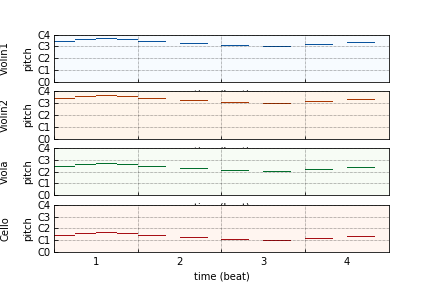
\includegraphics[width=\linewidth]{figures/first_bar.png}
  \caption{Pianoroll visualization of the first measure of
    Beethoven's Serioso String Quartet in F Minor}
  \label{pianoroll}
  \Description{A pianoroll representation of cello, viola and violin
    parts from a Beethoven piece.}
\end{figure}

\begin{figure}[h]
  \centering
  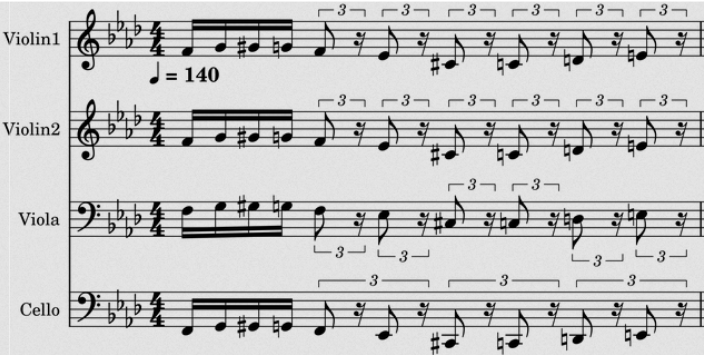
\includegraphics[width=\linewidth]{figures/first_bar_sheet.png}
  \caption{Sheet music of the first measure of Beethoven's Serioso
    String Quartet in F Minor}
  \label{sheet}
  \Description{A measure of sheet music cello, viola, and violin parts
    from Beethoven piece.}
\end{figure}

\subsection{Model Design}

The model is a recurrent variational autoencoder; both Long Short-Term
Memory (LSTM) and Gated Recurrent Unit (GRU) cell types were tested
but this choice did not make a significant difference in the results.

The encoder model utilizes an embedding layer to encode the note pitch
integers as vectors; embedding vector length is a tunable
hyperparameter and we found the best results with it set to 8. Then
two LSTM layers, with a dropout layer in between, convert the
sequences into latent codes, which are modeled as a multidimensional
Gaussian distribution $z$, produced by the encoder output Lambda layer
(Figure \ref{decoder}).

The decoder model samples from the latent space $z$ with the
distribution parameterized by the $\mu$ and $log(\sigma)$ values
learned by the encoder, and then utilizes two LSTM layers with a
dropout layer between them to generate sequences from the latent
codes. Then the network splits into four parallel outputs, one per
instrument track, where a fully connected layer with softmax
activation is used to select the most probable note value for the
the current track at the each time step (Figure \ref{decoder}).

\begin{figure}[h]
  \centering
  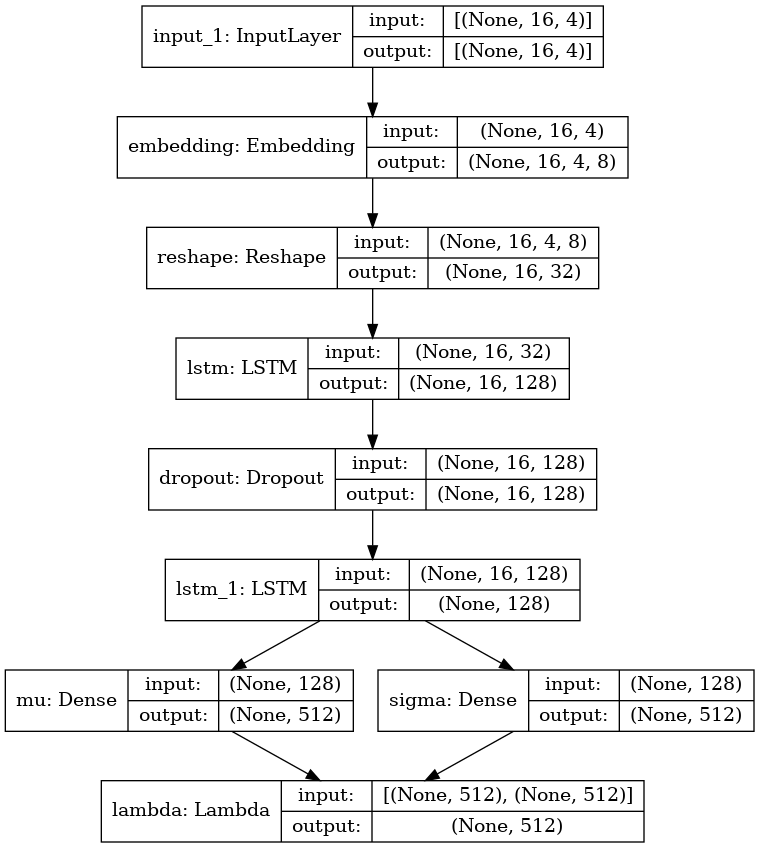
\includegraphics[width=\linewidth]{figures/encoder.png}
  \caption{A directed graph diagram of the encoder network.}
  \label{encoder}
\end{figure}


\begin{figure}[h]
  \centering
  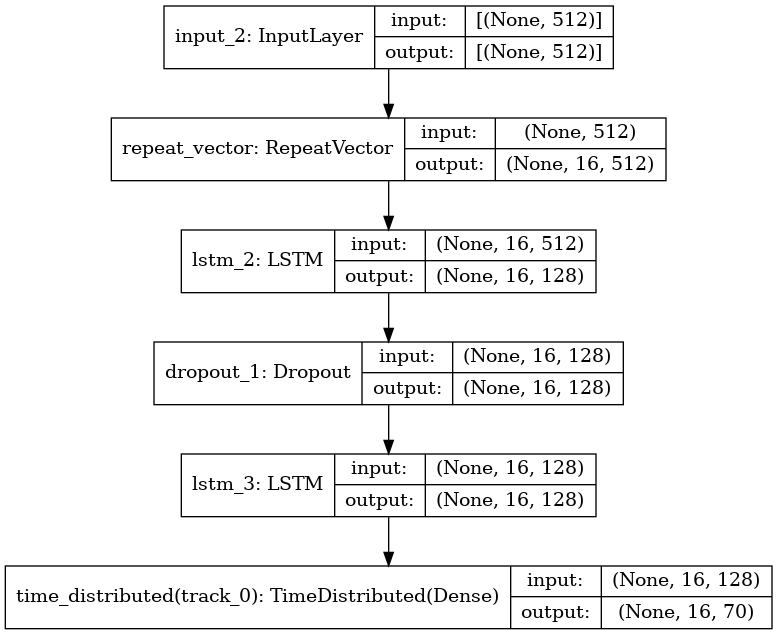
\includegraphics[width=\linewidth]{figures/decoder.png}
  \caption{A directed graph diagram of the decoder network (only one
    of four parallel output layers shown).}
  \label{decoder}
\end{figure}


The autoencoder reconstruction loss function is sparse categorical
cross-entropy, which is added to the Kullback-Leibler divergence of
the approximate posterior distribution from a multivariate Gaussian
distribution with mean 0 and standard deviation 1, resulting in the
(negative) evidence lower bound (ELBO) loss (Equation \ref{nelbo}),
which is a standard variational autoencoder loss function. This loss
function is applied to each track independently and then summed across
all four tracks with equal weight.

\begin{equation}
  \label{nelbo}
\mathbb{E}[log{p_\theta}(x|z)]-\mathbb{KL}(q_\lambda(z|x)||p(z))
\end{equation}

where $\lambda$ and $\theta$ represent the encoder and decoder
parameters respectively, while $q_\lambda(z|x)$ represents the
encoder, which approximates the true posterior probability $p(z|x)$,
and $p_\theta(x|z)$ represents the decoder, which parameterizes the
likelihood $p(x|z)$ \cite{roberts_hierarchical_2018}.



\subsection{Model Experimentation}

The following hyperparameters were tuned, with tested values listed
and best parameters in \textbf{bold}:

\begin{itemize}
  \tightlist
  \item batch size: \textbf{32}, 64, 96
  \item learning rate: 0.001, \textbf{0.0002}
  \item recurrent layer type: LSTM, GRU (made no difference)
  \item recurrent encoder layer directions: \textbf{unidirectional}, bidirectional
  \item recurrent layer cells: 64, \textbf{128}, 256
  \item latent code dimension: 128, 256, \textbf{512}
  \item embedding dimension: 4, \textbf{8}, 16
  \item dropout rate: 0.2, 0.4, \textbf{0.5}
  \item time steps per beat (quarter note): \textbf{4}, 8
  \item beats per phrase: \textbf{4}, 8
\end{itemize}

Each model was trained for up to 500 epochs with an early stopping
patience of 20 epochs. The model was cross-validated on 10\% of the
training data after each epoch. The best model was selected by a
combination of validation loss and listening to hand-picked sample
reconstructions and interpolations.

Data augmentation was also tested--\cite{oore_this_2018} suggests
augmentation via pitch shifting each training example up or down by up
to six semitones in order to create additional training examples and
reduce overfitting, so we followed that recommendation and used it to
double the size of the training dataset. As a result, we saw much
lower validation losses (compare Figure \ref{loss} and Figure
\ref{loss_augment} and a small but noticeable improvement in the
fidelity of the song reconstructions, suggesting that this method was
effective in reducing overfitting.

\begin{figure}[htbp]
    \begin{center}
        \scalebox{0.5}{%% Creator: Matplotlib, PGF backend
%%
%% To include the figure in your LaTeX document, write
%%   \input{<filename>.pgf}
%%
%% Make sure the required packages are loaded in your preamble
%%   \usepackage{pgf}
%%
%% Figures using additional raster images can only be included by \input if
%% they are in the same directory as the main LaTeX file. For loading figures
%% from other directories you can use the `import` package
%%   \usepackage{import}
%%
%% and then include the figures with
%%   \import{<path to file>}{<filename>.pgf}
%%
%% Matplotlib used the following preamble
%%   \usepackage{fontspec}
%%   \setmainfont{DejaVuSerif.ttf}[Path=\detokenize{/home/alex/miniconda3/envs/musiclearn/lib/python3.9/site-packages/matplotlib/mpl-data/fonts/ttf/}]
%%   \setsansfont{DejaVuSans.ttf}[Path=\detokenize{/home/alex/miniconda3/envs/musiclearn/lib/python3.9/site-packages/matplotlib/mpl-data/fonts/ttf/}]
%%   \setmonofont{DejaVuSansMono.ttf}[Path=\detokenize{/home/alex/miniconda3/envs/musiclearn/lib/python3.9/site-packages/matplotlib/mpl-data/fonts/ttf/}]
%%
\begingroup%
\makeatletter%
\begin{pgfpicture}%
\pgfpathrectangle{\pgfpointorigin}{\pgfqpoint{6.400000in}{4.800000in}}%
\pgfusepath{use as bounding box, clip}%
\begin{pgfscope}%
\pgfsetbuttcap%
\pgfsetmiterjoin%
\definecolor{currentfill}{rgb}{1.000000,1.000000,1.000000}%
\pgfsetfillcolor{currentfill}%
\pgfsetlinewidth{0.000000pt}%
\definecolor{currentstroke}{rgb}{1.000000,1.000000,1.000000}%
\pgfsetstrokecolor{currentstroke}%
\pgfsetdash{}{0pt}%
\pgfpathmoveto{\pgfqpoint{0.000000in}{0.000000in}}%
\pgfpathlineto{\pgfqpoint{6.400000in}{0.000000in}}%
\pgfpathlineto{\pgfqpoint{6.400000in}{4.800000in}}%
\pgfpathlineto{\pgfqpoint{0.000000in}{4.800000in}}%
\pgfpathclose%
\pgfusepath{fill}%
\end{pgfscope}%
\begin{pgfscope}%
\pgfsetbuttcap%
\pgfsetmiterjoin%
\definecolor{currentfill}{rgb}{1.000000,1.000000,1.000000}%
\pgfsetfillcolor{currentfill}%
\pgfsetlinewidth{0.000000pt}%
\definecolor{currentstroke}{rgb}{0.000000,0.000000,0.000000}%
\pgfsetstrokecolor{currentstroke}%
\pgfsetstrokeopacity{0.000000}%
\pgfsetdash{}{0pt}%
\pgfpathmoveto{\pgfqpoint{0.613921in}{0.571603in}}%
\pgfpathlineto{\pgfqpoint{6.250000in}{0.571603in}}%
\pgfpathlineto{\pgfqpoint{6.250000in}{4.650000in}}%
\pgfpathlineto{\pgfqpoint{0.613921in}{4.650000in}}%
\pgfpathclose%
\pgfusepath{fill}%
\end{pgfscope}%
\begin{pgfscope}%
\pgfsetbuttcap%
\pgfsetroundjoin%
\definecolor{currentfill}{rgb}{0.000000,0.000000,0.000000}%
\pgfsetfillcolor{currentfill}%
\pgfsetlinewidth{0.803000pt}%
\definecolor{currentstroke}{rgb}{0.000000,0.000000,0.000000}%
\pgfsetstrokecolor{currentstroke}%
\pgfsetdash{}{0pt}%
\pgfsys@defobject{currentmarker}{\pgfqpoint{0.000000in}{-0.048611in}}{\pgfqpoint{0.000000in}{0.000000in}}{%
\pgfpathmoveto{\pgfqpoint{0.000000in}{0.000000in}}%
\pgfpathlineto{\pgfqpoint{0.000000in}{-0.048611in}}%
\pgfusepath{stroke,fill}%
}%
\begin{pgfscope}%
\pgfsys@transformshift{0.870107in}{0.571603in}%
\pgfsys@useobject{currentmarker}{}%
\end{pgfscope}%
\end{pgfscope}%
\begin{pgfscope}%
\definecolor{textcolor}{rgb}{0.000000,0.000000,0.000000}%
\pgfsetstrokecolor{textcolor}%
\pgfsetfillcolor{textcolor}%
\pgftext[x=0.870107in,y=0.474381in,,top]{\color{textcolor}\sffamily\fontsize{10.000000}{12.000000}\selectfont 0}%
\end{pgfscope}%
\begin{pgfscope}%
\pgfsetbuttcap%
\pgfsetroundjoin%
\definecolor{currentfill}{rgb}{0.000000,0.000000,0.000000}%
\pgfsetfillcolor{currentfill}%
\pgfsetlinewidth{0.803000pt}%
\definecolor{currentstroke}{rgb}{0.000000,0.000000,0.000000}%
\pgfsetstrokecolor{currentstroke}%
\pgfsetdash{}{0pt}%
\pgfsys@defobject{currentmarker}{\pgfqpoint{0.000000in}{-0.048611in}}{\pgfqpoint{0.000000in}{0.000000in}}{%
\pgfpathmoveto{\pgfqpoint{0.000000in}{0.000000in}}%
\pgfpathlineto{\pgfqpoint{0.000000in}{-0.048611in}}%
\pgfusepath{stroke,fill}%
}%
\begin{pgfscope}%
\pgfsys@transformshift{1.969615in}{0.571603in}%
\pgfsys@useobject{currentmarker}{}%
\end{pgfscope}%
\end{pgfscope}%
\begin{pgfscope}%
\definecolor{textcolor}{rgb}{0.000000,0.000000,0.000000}%
\pgfsetstrokecolor{textcolor}%
\pgfsetfillcolor{textcolor}%
\pgftext[x=1.969615in,y=0.474381in,,top]{\color{textcolor}\sffamily\fontsize{10.000000}{12.000000}\selectfont 100}%
\end{pgfscope}%
\begin{pgfscope}%
\pgfsetbuttcap%
\pgfsetroundjoin%
\definecolor{currentfill}{rgb}{0.000000,0.000000,0.000000}%
\pgfsetfillcolor{currentfill}%
\pgfsetlinewidth{0.803000pt}%
\definecolor{currentstroke}{rgb}{0.000000,0.000000,0.000000}%
\pgfsetstrokecolor{currentstroke}%
\pgfsetdash{}{0pt}%
\pgfsys@defobject{currentmarker}{\pgfqpoint{0.000000in}{-0.048611in}}{\pgfqpoint{0.000000in}{0.000000in}}{%
\pgfpathmoveto{\pgfqpoint{0.000000in}{0.000000in}}%
\pgfpathlineto{\pgfqpoint{0.000000in}{-0.048611in}}%
\pgfusepath{stroke,fill}%
}%
\begin{pgfscope}%
\pgfsys@transformshift{3.069123in}{0.571603in}%
\pgfsys@useobject{currentmarker}{}%
\end{pgfscope}%
\end{pgfscope}%
\begin{pgfscope}%
\definecolor{textcolor}{rgb}{0.000000,0.000000,0.000000}%
\pgfsetstrokecolor{textcolor}%
\pgfsetfillcolor{textcolor}%
\pgftext[x=3.069123in,y=0.474381in,,top]{\color{textcolor}\sffamily\fontsize{10.000000}{12.000000}\selectfont 200}%
\end{pgfscope}%
\begin{pgfscope}%
\pgfsetbuttcap%
\pgfsetroundjoin%
\definecolor{currentfill}{rgb}{0.000000,0.000000,0.000000}%
\pgfsetfillcolor{currentfill}%
\pgfsetlinewidth{0.803000pt}%
\definecolor{currentstroke}{rgb}{0.000000,0.000000,0.000000}%
\pgfsetstrokecolor{currentstroke}%
\pgfsetdash{}{0pt}%
\pgfsys@defobject{currentmarker}{\pgfqpoint{0.000000in}{-0.048611in}}{\pgfqpoint{0.000000in}{0.000000in}}{%
\pgfpathmoveto{\pgfqpoint{0.000000in}{0.000000in}}%
\pgfpathlineto{\pgfqpoint{0.000000in}{-0.048611in}}%
\pgfusepath{stroke,fill}%
}%
\begin{pgfscope}%
\pgfsys@transformshift{4.168631in}{0.571603in}%
\pgfsys@useobject{currentmarker}{}%
\end{pgfscope}%
\end{pgfscope}%
\begin{pgfscope}%
\definecolor{textcolor}{rgb}{0.000000,0.000000,0.000000}%
\pgfsetstrokecolor{textcolor}%
\pgfsetfillcolor{textcolor}%
\pgftext[x=4.168631in,y=0.474381in,,top]{\color{textcolor}\sffamily\fontsize{10.000000}{12.000000}\selectfont 300}%
\end{pgfscope}%
\begin{pgfscope}%
\pgfsetbuttcap%
\pgfsetroundjoin%
\definecolor{currentfill}{rgb}{0.000000,0.000000,0.000000}%
\pgfsetfillcolor{currentfill}%
\pgfsetlinewidth{0.803000pt}%
\definecolor{currentstroke}{rgb}{0.000000,0.000000,0.000000}%
\pgfsetstrokecolor{currentstroke}%
\pgfsetdash{}{0pt}%
\pgfsys@defobject{currentmarker}{\pgfqpoint{0.000000in}{-0.048611in}}{\pgfqpoint{0.000000in}{0.000000in}}{%
\pgfpathmoveto{\pgfqpoint{0.000000in}{0.000000in}}%
\pgfpathlineto{\pgfqpoint{0.000000in}{-0.048611in}}%
\pgfusepath{stroke,fill}%
}%
\begin{pgfscope}%
\pgfsys@transformshift{5.268139in}{0.571603in}%
\pgfsys@useobject{currentmarker}{}%
\end{pgfscope}%
\end{pgfscope}%
\begin{pgfscope}%
\definecolor{textcolor}{rgb}{0.000000,0.000000,0.000000}%
\pgfsetstrokecolor{textcolor}%
\pgfsetfillcolor{textcolor}%
\pgftext[x=5.268139in,y=0.474381in,,top]{\color{textcolor}\sffamily\fontsize{10.000000}{12.000000}\selectfont 400}%
\end{pgfscope}%
\begin{pgfscope}%
\definecolor{textcolor}{rgb}{0.000000,0.000000,0.000000}%
\pgfsetstrokecolor{textcolor}%
\pgfsetfillcolor{textcolor}%
\pgftext[x=3.431961in,y=0.284413in,,top]{\color{textcolor}\sffamily\fontsize{10.000000}{12.000000}\selectfont Training Epochs}%
\end{pgfscope}%
\begin{pgfscope}%
\pgfsetbuttcap%
\pgfsetroundjoin%
\definecolor{currentfill}{rgb}{0.000000,0.000000,0.000000}%
\pgfsetfillcolor{currentfill}%
\pgfsetlinewidth{0.803000pt}%
\definecolor{currentstroke}{rgb}{0.000000,0.000000,0.000000}%
\pgfsetstrokecolor{currentstroke}%
\pgfsetdash{}{0pt}%
\pgfsys@defobject{currentmarker}{\pgfqpoint{-0.048611in}{0.000000in}}{\pgfqpoint{-0.000000in}{0.000000in}}{%
\pgfpathmoveto{\pgfqpoint{-0.000000in}{0.000000in}}%
\pgfpathlineto{\pgfqpoint{-0.048611in}{0.000000in}}%
\pgfusepath{stroke,fill}%
}%
\begin{pgfscope}%
\pgfsys@transformshift{0.613921in}{0.571603in}%
\pgfsys@useobject{currentmarker}{}%
\end{pgfscope}%
\end{pgfscope}%
\begin{pgfscope}%
\definecolor{textcolor}{rgb}{0.000000,0.000000,0.000000}%
\pgfsetstrokecolor{textcolor}%
\pgfsetfillcolor{textcolor}%
\pgftext[x=0.428334in, y=0.518842in, left, base]{\color{textcolor}\sffamily\fontsize{10.000000}{12.000000}\selectfont 0}%
\end{pgfscope}%
\begin{pgfscope}%
\pgfsetbuttcap%
\pgfsetroundjoin%
\definecolor{currentfill}{rgb}{0.000000,0.000000,0.000000}%
\pgfsetfillcolor{currentfill}%
\pgfsetlinewidth{0.803000pt}%
\definecolor{currentstroke}{rgb}{0.000000,0.000000,0.000000}%
\pgfsetstrokecolor{currentstroke}%
\pgfsetdash{}{0pt}%
\pgfsys@defobject{currentmarker}{\pgfqpoint{-0.048611in}{0.000000in}}{\pgfqpoint{-0.000000in}{0.000000in}}{%
\pgfpathmoveto{\pgfqpoint{-0.000000in}{0.000000in}}%
\pgfpathlineto{\pgfqpoint{-0.048611in}{0.000000in}}%
\pgfusepath{stroke,fill}%
}%
\begin{pgfscope}%
\pgfsys@transformshift{0.613921in}{1.284436in}%
\pgfsys@useobject{currentmarker}{}%
\end{pgfscope}%
\end{pgfscope}%
\begin{pgfscope}%
\definecolor{textcolor}{rgb}{0.000000,0.000000,0.000000}%
\pgfsetstrokecolor{textcolor}%
\pgfsetfillcolor{textcolor}%
\pgftext[x=0.428334in, y=1.231674in, left, base]{\color{textcolor}\sffamily\fontsize{10.000000}{12.000000}\selectfont 2}%
\end{pgfscope}%
\begin{pgfscope}%
\pgfsetbuttcap%
\pgfsetroundjoin%
\definecolor{currentfill}{rgb}{0.000000,0.000000,0.000000}%
\pgfsetfillcolor{currentfill}%
\pgfsetlinewidth{0.803000pt}%
\definecolor{currentstroke}{rgb}{0.000000,0.000000,0.000000}%
\pgfsetstrokecolor{currentstroke}%
\pgfsetdash{}{0pt}%
\pgfsys@defobject{currentmarker}{\pgfqpoint{-0.048611in}{0.000000in}}{\pgfqpoint{-0.000000in}{0.000000in}}{%
\pgfpathmoveto{\pgfqpoint{-0.000000in}{0.000000in}}%
\pgfpathlineto{\pgfqpoint{-0.048611in}{0.000000in}}%
\pgfusepath{stroke,fill}%
}%
\begin{pgfscope}%
\pgfsys@transformshift{0.613921in}{1.997268in}%
\pgfsys@useobject{currentmarker}{}%
\end{pgfscope}%
\end{pgfscope}%
\begin{pgfscope}%
\definecolor{textcolor}{rgb}{0.000000,0.000000,0.000000}%
\pgfsetstrokecolor{textcolor}%
\pgfsetfillcolor{textcolor}%
\pgftext[x=0.428334in, y=1.944506in, left, base]{\color{textcolor}\sffamily\fontsize{10.000000}{12.000000}\selectfont 4}%
\end{pgfscope}%
\begin{pgfscope}%
\pgfsetbuttcap%
\pgfsetroundjoin%
\definecolor{currentfill}{rgb}{0.000000,0.000000,0.000000}%
\pgfsetfillcolor{currentfill}%
\pgfsetlinewidth{0.803000pt}%
\definecolor{currentstroke}{rgb}{0.000000,0.000000,0.000000}%
\pgfsetstrokecolor{currentstroke}%
\pgfsetdash{}{0pt}%
\pgfsys@defobject{currentmarker}{\pgfqpoint{-0.048611in}{0.000000in}}{\pgfqpoint{-0.000000in}{0.000000in}}{%
\pgfpathmoveto{\pgfqpoint{-0.000000in}{0.000000in}}%
\pgfpathlineto{\pgfqpoint{-0.048611in}{0.000000in}}%
\pgfusepath{stroke,fill}%
}%
\begin{pgfscope}%
\pgfsys@transformshift{0.613921in}{2.710100in}%
\pgfsys@useobject{currentmarker}{}%
\end{pgfscope}%
\end{pgfscope}%
\begin{pgfscope}%
\definecolor{textcolor}{rgb}{0.000000,0.000000,0.000000}%
\pgfsetstrokecolor{textcolor}%
\pgfsetfillcolor{textcolor}%
\pgftext[x=0.428334in, y=2.657339in, left, base]{\color{textcolor}\sffamily\fontsize{10.000000}{12.000000}\selectfont 6}%
\end{pgfscope}%
\begin{pgfscope}%
\pgfsetbuttcap%
\pgfsetroundjoin%
\definecolor{currentfill}{rgb}{0.000000,0.000000,0.000000}%
\pgfsetfillcolor{currentfill}%
\pgfsetlinewidth{0.803000pt}%
\definecolor{currentstroke}{rgb}{0.000000,0.000000,0.000000}%
\pgfsetstrokecolor{currentstroke}%
\pgfsetdash{}{0pt}%
\pgfsys@defobject{currentmarker}{\pgfqpoint{-0.048611in}{0.000000in}}{\pgfqpoint{-0.000000in}{0.000000in}}{%
\pgfpathmoveto{\pgfqpoint{-0.000000in}{0.000000in}}%
\pgfpathlineto{\pgfqpoint{-0.048611in}{0.000000in}}%
\pgfusepath{stroke,fill}%
}%
\begin{pgfscope}%
\pgfsys@transformshift{0.613921in}{3.422933in}%
\pgfsys@useobject{currentmarker}{}%
\end{pgfscope}%
\end{pgfscope}%
\begin{pgfscope}%
\definecolor{textcolor}{rgb}{0.000000,0.000000,0.000000}%
\pgfsetstrokecolor{textcolor}%
\pgfsetfillcolor{textcolor}%
\pgftext[x=0.428334in, y=3.370171in, left, base]{\color{textcolor}\sffamily\fontsize{10.000000}{12.000000}\selectfont 8}%
\end{pgfscope}%
\begin{pgfscope}%
\pgfsetbuttcap%
\pgfsetroundjoin%
\definecolor{currentfill}{rgb}{0.000000,0.000000,0.000000}%
\pgfsetfillcolor{currentfill}%
\pgfsetlinewidth{0.803000pt}%
\definecolor{currentstroke}{rgb}{0.000000,0.000000,0.000000}%
\pgfsetstrokecolor{currentstroke}%
\pgfsetdash{}{0pt}%
\pgfsys@defobject{currentmarker}{\pgfqpoint{-0.048611in}{0.000000in}}{\pgfqpoint{-0.000000in}{0.000000in}}{%
\pgfpathmoveto{\pgfqpoint{-0.000000in}{0.000000in}}%
\pgfpathlineto{\pgfqpoint{-0.048611in}{0.000000in}}%
\pgfusepath{stroke,fill}%
}%
\begin{pgfscope}%
\pgfsys@transformshift{0.613921in}{4.135765in}%
\pgfsys@useobject{currentmarker}{}%
\end{pgfscope}%
\end{pgfscope}%
\begin{pgfscope}%
\definecolor{textcolor}{rgb}{0.000000,0.000000,0.000000}%
\pgfsetstrokecolor{textcolor}%
\pgfsetfillcolor{textcolor}%
\pgftext[x=0.339968in, y=4.083003in, left, base]{\color{textcolor}\sffamily\fontsize{10.000000}{12.000000}\selectfont 10}%
\end{pgfscope}%
\begin{pgfscope}%
\definecolor{textcolor}{rgb}{0.000000,0.000000,0.000000}%
\pgfsetstrokecolor{textcolor}%
\pgfsetfillcolor{textcolor}%
\pgftext[x=0.284413in,y=2.610802in,,bottom,rotate=90.000000]{\color{textcolor}\sffamily\fontsize{10.000000}{12.000000}\selectfont Loss Score}%
\end{pgfscope}%
\begin{pgfscope}%
\pgfpathrectangle{\pgfqpoint{0.613921in}{0.571603in}}{\pgfqpoint{5.636079in}{4.078397in}}%
\pgfusepath{clip}%
\pgfsetrectcap%
\pgfsetroundjoin%
\pgfsetlinewidth{1.505625pt}%
\definecolor{currentstroke}{rgb}{0.121569,0.466667,0.705882}%
\pgfsetstrokecolor{currentstroke}%
\pgfsetdash{}{0pt}%
\pgfpathmoveto{\pgfqpoint{0.870107in}{4.508442in}}%
\pgfpathlineto{\pgfqpoint{0.881102in}{3.561162in}}%
\pgfpathlineto{\pgfqpoint{0.892097in}{3.501197in}}%
\pgfpathlineto{\pgfqpoint{0.903092in}{3.417093in}}%
\pgfpathlineto{\pgfqpoint{0.925082in}{3.318037in}}%
\pgfpathlineto{\pgfqpoint{0.936077in}{3.288336in}}%
\pgfpathlineto{\pgfqpoint{0.947072in}{3.271347in}}%
\pgfpathlineto{\pgfqpoint{0.969062in}{3.252627in}}%
\pgfpathlineto{\pgfqpoint{0.980057in}{3.245592in}}%
\pgfpathlineto{\pgfqpoint{0.991053in}{3.243777in}}%
\pgfpathlineto{\pgfqpoint{1.002048in}{3.234504in}}%
\pgfpathlineto{\pgfqpoint{1.013043in}{3.227831in}}%
\pgfpathlineto{\pgfqpoint{1.024038in}{3.218981in}}%
\pgfpathlineto{\pgfqpoint{1.035033in}{3.199488in}}%
\pgfpathlineto{\pgfqpoint{1.057023in}{3.175679in}}%
\pgfpathlineto{\pgfqpoint{1.068018in}{3.168918in}}%
\pgfpathlineto{\pgfqpoint{1.079013in}{3.159672in}}%
\pgfpathlineto{\pgfqpoint{1.090008in}{3.153281in}}%
\pgfpathlineto{\pgfqpoint{1.122994in}{3.121844in}}%
\pgfpathlineto{\pgfqpoint{1.144984in}{3.091997in}}%
\pgfpathlineto{\pgfqpoint{1.155979in}{3.082991in}}%
\pgfpathlineto{\pgfqpoint{1.166974in}{3.077224in}}%
\pgfpathlineto{\pgfqpoint{1.177969in}{3.068529in}}%
\pgfpathlineto{\pgfqpoint{1.210954in}{3.051394in}}%
\pgfpathlineto{\pgfqpoint{1.221949in}{3.048560in}}%
\pgfpathlineto{\pgfqpoint{1.232944in}{3.043442in}}%
\pgfpathlineto{\pgfqpoint{1.243939in}{3.040321in}}%
\pgfpathlineto{\pgfqpoint{1.254934in}{3.033842in}}%
\pgfpathlineto{\pgfqpoint{1.265930in}{3.030857in}}%
\pgfpathlineto{\pgfqpoint{1.276925in}{3.029260in}}%
\pgfpathlineto{\pgfqpoint{1.287920in}{3.023344in}}%
\pgfpathlineto{\pgfqpoint{1.309910in}{3.014950in}}%
\pgfpathlineto{\pgfqpoint{1.320905in}{3.008435in}}%
\pgfpathlineto{\pgfqpoint{1.342895in}{2.999829in}}%
\pgfpathlineto{\pgfqpoint{1.353890in}{2.991656in}}%
\pgfpathlineto{\pgfqpoint{1.364885in}{2.986264in}}%
\pgfpathlineto{\pgfqpoint{1.375880in}{2.979545in}}%
\pgfpathlineto{\pgfqpoint{1.386875in}{2.970472in}}%
\pgfpathlineto{\pgfqpoint{1.397871in}{2.981416in}}%
\pgfpathlineto{\pgfqpoint{1.408866in}{2.963223in}}%
\pgfpathlineto{\pgfqpoint{1.419861in}{2.952493in}}%
\pgfpathlineto{\pgfqpoint{1.430856in}{2.944018in}}%
\pgfpathlineto{\pgfqpoint{1.463841in}{2.913376in}}%
\pgfpathlineto{\pgfqpoint{1.496826in}{2.890154in}}%
\pgfpathlineto{\pgfqpoint{1.507821in}{2.883113in}}%
\pgfpathlineto{\pgfqpoint{1.540807in}{2.866848in}}%
\pgfpathlineto{\pgfqpoint{1.551802in}{2.861588in}}%
\pgfpathlineto{\pgfqpoint{1.573792in}{2.846992in}}%
\pgfpathlineto{\pgfqpoint{1.584787in}{2.842346in}}%
\pgfpathlineto{\pgfqpoint{1.595782in}{2.834635in}}%
\pgfpathlineto{\pgfqpoint{1.628767in}{2.819527in}}%
\pgfpathlineto{\pgfqpoint{1.650757in}{2.808742in}}%
\pgfpathlineto{\pgfqpoint{1.672748in}{2.801499in}}%
\pgfpathlineto{\pgfqpoint{1.694738in}{2.790108in}}%
\pgfpathlineto{\pgfqpoint{1.705733in}{2.785337in}}%
\pgfpathlineto{\pgfqpoint{1.716728in}{2.782910in}}%
\pgfpathlineto{\pgfqpoint{1.837674in}{2.732908in}}%
\pgfpathlineto{\pgfqpoint{1.881654in}{2.711938in}}%
\pgfpathlineto{\pgfqpoint{1.892649in}{2.703924in}}%
\pgfpathlineto{\pgfqpoint{1.903644in}{2.698016in}}%
\pgfpathlineto{\pgfqpoint{1.914639in}{2.693761in}}%
\pgfpathlineto{\pgfqpoint{1.925634in}{2.687911in}}%
\pgfpathlineto{\pgfqpoint{1.947625in}{2.680051in}}%
\pgfpathlineto{\pgfqpoint{1.958620in}{2.673152in}}%
\pgfpathlineto{\pgfqpoint{1.969615in}{2.668182in}}%
\pgfpathlineto{\pgfqpoint{1.980610in}{2.664704in}}%
\pgfpathlineto{\pgfqpoint{1.991605in}{2.657056in}}%
\pgfpathlineto{\pgfqpoint{2.002600in}{2.654963in}}%
\pgfpathlineto{\pgfqpoint{2.013595in}{2.649309in}}%
\pgfpathlineto{\pgfqpoint{2.024590in}{2.646932in}}%
\pgfpathlineto{\pgfqpoint{2.035585in}{2.640916in}}%
\pgfpathlineto{\pgfqpoint{2.057575in}{2.632995in}}%
\pgfpathlineto{\pgfqpoint{2.068571in}{2.628552in}}%
\pgfpathlineto{\pgfqpoint{2.090561in}{2.618003in}}%
\pgfpathlineto{\pgfqpoint{2.123546in}{2.601097in}}%
\pgfpathlineto{\pgfqpoint{2.134541in}{2.591831in}}%
\pgfpathlineto{\pgfqpoint{2.178521in}{2.568223in}}%
\pgfpathlineto{\pgfqpoint{2.189516in}{2.566736in}}%
\pgfpathlineto{\pgfqpoint{2.222502in}{2.537095in}}%
\pgfpathlineto{\pgfqpoint{2.233497in}{2.535844in}}%
\pgfpathlineto{\pgfqpoint{2.244492in}{2.524748in}}%
\pgfpathlineto{\pgfqpoint{2.255487in}{2.526083in}}%
\pgfpathlineto{\pgfqpoint{2.266482in}{2.512844in}}%
\pgfpathlineto{\pgfqpoint{2.277477in}{2.504797in}}%
\pgfpathlineto{\pgfqpoint{2.288472in}{2.499314in}}%
\pgfpathlineto{\pgfqpoint{2.299467in}{2.504402in}}%
\pgfpathlineto{\pgfqpoint{2.310462in}{2.492638in}}%
\pgfpathlineto{\pgfqpoint{2.321457in}{2.484785in}}%
\pgfpathlineto{\pgfqpoint{2.332452in}{2.485303in}}%
\pgfpathlineto{\pgfqpoint{2.343448in}{2.474221in}}%
\pgfpathlineto{\pgfqpoint{2.354443in}{2.470592in}}%
\pgfpathlineto{\pgfqpoint{2.365438in}{2.462932in}}%
\pgfpathlineto{\pgfqpoint{2.376433in}{2.464306in}}%
\pgfpathlineto{\pgfqpoint{2.387428in}{2.452472in}}%
\pgfpathlineto{\pgfqpoint{2.398423in}{2.447242in}}%
\pgfpathlineto{\pgfqpoint{2.409418in}{2.447974in}}%
\pgfpathlineto{\pgfqpoint{2.420413in}{2.436604in}}%
\pgfpathlineto{\pgfqpoint{2.431408in}{2.435415in}}%
\pgfpathlineto{\pgfqpoint{2.442403in}{2.425699in}}%
\pgfpathlineto{\pgfqpoint{2.453398in}{2.422138in}}%
\pgfpathlineto{\pgfqpoint{2.464393in}{2.421033in}}%
\pgfpathlineto{\pgfqpoint{2.475389in}{2.417695in}}%
\pgfpathlineto{\pgfqpoint{2.486384in}{2.407221in}}%
\pgfpathlineto{\pgfqpoint{2.497379in}{2.407287in}}%
\pgfpathlineto{\pgfqpoint{2.519369in}{2.395793in}}%
\pgfpathlineto{\pgfqpoint{2.530364in}{2.391421in}}%
\pgfpathlineto{\pgfqpoint{2.541359in}{2.383705in}}%
\pgfpathlineto{\pgfqpoint{2.552354in}{2.378183in}}%
\pgfpathlineto{\pgfqpoint{2.563349in}{2.379521in}}%
\pgfpathlineto{\pgfqpoint{2.574344in}{2.362907in}}%
\pgfpathlineto{\pgfqpoint{2.585339in}{2.353452in}}%
\pgfpathlineto{\pgfqpoint{2.596334in}{2.339980in}}%
\pgfpathlineto{\pgfqpoint{2.618325in}{2.322902in}}%
\pgfpathlineto{\pgfqpoint{2.629320in}{2.309577in}}%
\pgfpathlineto{\pgfqpoint{2.640315in}{2.298855in}}%
\pgfpathlineto{\pgfqpoint{2.651310in}{2.291788in}}%
\pgfpathlineto{\pgfqpoint{2.662305in}{2.289009in}}%
\pgfpathlineto{\pgfqpoint{2.673300in}{2.281418in}}%
\pgfpathlineto{\pgfqpoint{2.706285in}{2.267120in}}%
\pgfpathlineto{\pgfqpoint{2.717280in}{2.262113in}}%
\pgfpathlineto{\pgfqpoint{2.728275in}{2.258940in}}%
\pgfpathlineto{\pgfqpoint{2.739270in}{2.254081in}}%
\pgfpathlineto{\pgfqpoint{2.750266in}{2.251159in}}%
\pgfpathlineto{\pgfqpoint{2.761261in}{2.245843in}}%
\pgfpathlineto{\pgfqpoint{2.772256in}{2.244591in}}%
\pgfpathlineto{\pgfqpoint{2.783251in}{2.239147in}}%
\pgfpathlineto{\pgfqpoint{2.794246in}{2.236009in}}%
\pgfpathlineto{\pgfqpoint{2.805241in}{2.230146in}}%
\pgfpathlineto{\pgfqpoint{2.816236in}{2.227270in}}%
\pgfpathlineto{\pgfqpoint{2.827231in}{2.228199in}}%
\pgfpathlineto{\pgfqpoint{2.849221in}{2.219623in}}%
\pgfpathlineto{\pgfqpoint{2.860216in}{2.214092in}}%
\pgfpathlineto{\pgfqpoint{2.871211in}{2.213747in}}%
\pgfpathlineto{\pgfqpoint{2.882207in}{2.209187in}}%
\pgfpathlineto{\pgfqpoint{2.904197in}{2.202894in}}%
\pgfpathlineto{\pgfqpoint{2.915192in}{2.202587in}}%
\pgfpathlineto{\pgfqpoint{2.926187in}{2.197314in}}%
\pgfpathlineto{\pgfqpoint{2.937182in}{2.196038in}}%
\pgfpathlineto{\pgfqpoint{2.948177in}{2.190890in}}%
\pgfpathlineto{\pgfqpoint{2.959172in}{2.187138in}}%
\pgfpathlineto{\pgfqpoint{2.970167in}{2.186206in}}%
\pgfpathlineto{\pgfqpoint{2.981162in}{2.181959in}}%
\pgfpathlineto{\pgfqpoint{2.992157in}{2.180901in}}%
\pgfpathlineto{\pgfqpoint{3.014148in}{2.173542in}}%
\pgfpathlineto{\pgfqpoint{3.025143in}{2.171621in}}%
\pgfpathlineto{\pgfqpoint{3.069123in}{2.158639in}}%
\pgfpathlineto{\pgfqpoint{3.080118in}{2.157380in}}%
\pgfpathlineto{\pgfqpoint{3.102108in}{2.151420in}}%
\pgfpathlineto{\pgfqpoint{3.113103in}{2.146835in}}%
\pgfpathlineto{\pgfqpoint{3.124098in}{2.146320in}}%
\pgfpathlineto{\pgfqpoint{3.146089in}{2.138610in}}%
\pgfpathlineto{\pgfqpoint{3.168079in}{2.133184in}}%
\pgfpathlineto{\pgfqpoint{3.190069in}{2.125617in}}%
\pgfpathlineto{\pgfqpoint{3.212059in}{2.123457in}}%
\pgfpathlineto{\pgfqpoint{3.223054in}{2.120773in}}%
\pgfpathlineto{\pgfqpoint{3.234049in}{2.115986in}}%
\pgfpathlineto{\pgfqpoint{3.245044in}{2.112497in}}%
\pgfpathlineto{\pgfqpoint{3.256039in}{2.110688in}}%
\pgfpathlineto{\pgfqpoint{3.267034in}{2.106439in}}%
\pgfpathlineto{\pgfqpoint{3.300020in}{2.100763in}}%
\pgfpathlineto{\pgfqpoint{3.333005in}{2.089211in}}%
\pgfpathlineto{\pgfqpoint{3.344000in}{2.087108in}}%
\pgfpathlineto{\pgfqpoint{3.354995in}{2.086676in}}%
\pgfpathlineto{\pgfqpoint{3.365990in}{2.080533in}}%
\pgfpathlineto{\pgfqpoint{3.376985in}{2.075722in}}%
\pgfpathlineto{\pgfqpoint{3.387980in}{2.073185in}}%
\pgfpathlineto{\pgfqpoint{3.398975in}{2.073936in}}%
\pgfpathlineto{\pgfqpoint{3.409970in}{2.067071in}}%
\pgfpathlineto{\pgfqpoint{3.431961in}{2.056784in}}%
\pgfpathlineto{\pgfqpoint{3.453951in}{2.049337in}}%
\pgfpathlineto{\pgfqpoint{3.464946in}{2.048418in}}%
\pgfpathlineto{\pgfqpoint{3.475941in}{2.040381in}}%
\pgfpathlineto{\pgfqpoint{3.508926in}{2.026860in}}%
\pgfpathlineto{\pgfqpoint{3.519921in}{2.027879in}}%
\pgfpathlineto{\pgfqpoint{3.530916in}{2.023514in}}%
\pgfpathlineto{\pgfqpoint{3.541911in}{2.017160in}}%
\pgfpathlineto{\pgfqpoint{3.563902in}{2.019213in}}%
\pgfpathlineto{\pgfqpoint{3.574897in}{2.012348in}}%
\pgfpathlineto{\pgfqpoint{3.585892in}{2.007316in}}%
\pgfpathlineto{\pgfqpoint{3.596887in}{2.005930in}}%
\pgfpathlineto{\pgfqpoint{3.607882in}{2.003070in}}%
\pgfpathlineto{\pgfqpoint{3.618877in}{2.002030in}}%
\pgfpathlineto{\pgfqpoint{3.629872in}{1.996969in}}%
\pgfpathlineto{\pgfqpoint{3.651862in}{1.991612in}}%
\pgfpathlineto{\pgfqpoint{3.662857in}{1.989055in}}%
\pgfpathlineto{\pgfqpoint{3.673852in}{1.984626in}}%
\pgfpathlineto{\pgfqpoint{3.684847in}{1.983103in}}%
\pgfpathlineto{\pgfqpoint{3.695843in}{1.983944in}}%
\pgfpathlineto{\pgfqpoint{3.706838in}{1.979917in}}%
\pgfpathlineto{\pgfqpoint{3.717833in}{1.978782in}}%
\pgfpathlineto{\pgfqpoint{3.739823in}{1.973574in}}%
\pgfpathlineto{\pgfqpoint{3.750818in}{1.976078in}}%
\pgfpathlineto{\pgfqpoint{3.761813in}{1.969307in}}%
\pgfpathlineto{\pgfqpoint{3.805793in}{1.957516in}}%
\pgfpathlineto{\pgfqpoint{3.816788in}{1.956535in}}%
\pgfpathlineto{\pgfqpoint{3.838779in}{1.951383in}}%
\pgfpathlineto{\pgfqpoint{3.860769in}{1.950023in}}%
\pgfpathlineto{\pgfqpoint{3.882759in}{1.946144in}}%
\pgfpathlineto{\pgfqpoint{3.893754in}{1.941221in}}%
\pgfpathlineto{\pgfqpoint{3.904749in}{1.938867in}}%
\pgfpathlineto{\pgfqpoint{3.915744in}{1.935284in}}%
\pgfpathlineto{\pgfqpoint{3.926739in}{1.934643in}}%
\pgfpathlineto{\pgfqpoint{3.937734in}{1.936538in}}%
\pgfpathlineto{\pgfqpoint{3.948729in}{1.931343in}}%
\pgfpathlineto{\pgfqpoint{3.970720in}{1.926483in}}%
\pgfpathlineto{\pgfqpoint{3.992710in}{1.922976in}}%
\pgfpathlineto{\pgfqpoint{4.003705in}{1.919712in}}%
\pgfpathlineto{\pgfqpoint{4.014700in}{1.918207in}}%
\pgfpathlineto{\pgfqpoint{4.025695in}{1.919368in}}%
\pgfpathlineto{\pgfqpoint{4.036690in}{1.914438in}}%
\pgfpathlineto{\pgfqpoint{4.047685in}{1.911920in}}%
\pgfpathlineto{\pgfqpoint{4.058680in}{1.912678in}}%
\pgfpathlineto{\pgfqpoint{4.069675in}{1.911611in}}%
\pgfpathlineto{\pgfqpoint{4.080670in}{1.908395in}}%
\pgfpathlineto{\pgfqpoint{4.091666in}{1.906591in}}%
\pgfpathlineto{\pgfqpoint{4.102661in}{1.906041in}}%
\pgfpathlineto{\pgfqpoint{4.113656in}{1.904265in}}%
\pgfpathlineto{\pgfqpoint{4.124651in}{1.899620in}}%
\pgfpathlineto{\pgfqpoint{4.146641in}{1.896501in}}%
\pgfpathlineto{\pgfqpoint{4.157636in}{1.893141in}}%
\pgfpathlineto{\pgfqpoint{4.179626in}{1.889398in}}%
\pgfpathlineto{\pgfqpoint{4.190621in}{1.889674in}}%
\pgfpathlineto{\pgfqpoint{4.201616in}{1.886307in}}%
\pgfpathlineto{\pgfqpoint{4.234602in}{1.880331in}}%
\pgfpathlineto{\pgfqpoint{4.245597in}{1.881047in}}%
\pgfpathlineto{\pgfqpoint{4.289577in}{1.872354in}}%
\pgfpathlineto{\pgfqpoint{4.300572in}{1.875346in}}%
\pgfpathlineto{\pgfqpoint{4.333557in}{1.865276in}}%
\pgfpathlineto{\pgfqpoint{4.344552in}{1.863354in}}%
\pgfpathlineto{\pgfqpoint{4.355547in}{1.864797in}}%
\pgfpathlineto{\pgfqpoint{4.366543in}{1.859038in}}%
\pgfpathlineto{\pgfqpoint{4.377538in}{1.861795in}}%
\pgfpathlineto{\pgfqpoint{4.399528in}{1.854357in}}%
\pgfpathlineto{\pgfqpoint{4.410523in}{1.855164in}}%
\pgfpathlineto{\pgfqpoint{4.432513in}{1.849137in}}%
\pgfpathlineto{\pgfqpoint{4.443508in}{1.851212in}}%
\pgfpathlineto{\pgfqpoint{4.454503in}{1.846487in}}%
\pgfpathlineto{\pgfqpoint{4.465498in}{1.847780in}}%
\pgfpathlineto{\pgfqpoint{4.476493in}{1.844679in}}%
\pgfpathlineto{\pgfqpoint{4.531469in}{1.838359in}}%
\pgfpathlineto{\pgfqpoint{4.542464in}{1.834128in}}%
\pgfpathlineto{\pgfqpoint{4.553459in}{1.837585in}}%
\pgfpathlineto{\pgfqpoint{4.586444in}{1.828114in}}%
\pgfpathlineto{\pgfqpoint{4.597439in}{1.829671in}}%
\pgfpathlineto{\pgfqpoint{4.608434in}{1.826128in}}%
\pgfpathlineto{\pgfqpoint{4.619429in}{1.824636in}}%
\pgfpathlineto{\pgfqpoint{4.630425in}{1.825320in}}%
\pgfpathlineto{\pgfqpoint{4.641420in}{1.821450in}}%
\pgfpathlineto{\pgfqpoint{4.663410in}{1.820311in}}%
\pgfpathlineto{\pgfqpoint{4.674405in}{1.820400in}}%
\pgfpathlineto{\pgfqpoint{4.685400in}{1.816302in}}%
\pgfpathlineto{\pgfqpoint{4.696395in}{1.813922in}}%
\pgfpathlineto{\pgfqpoint{4.707390in}{1.815843in}}%
\pgfpathlineto{\pgfqpoint{4.718385in}{1.812294in}}%
\pgfpathlineto{\pgfqpoint{4.729380in}{1.810951in}}%
\pgfpathlineto{\pgfqpoint{4.751370in}{1.805675in}}%
\pgfpathlineto{\pgfqpoint{4.762365in}{1.808120in}}%
\pgfpathlineto{\pgfqpoint{4.773361in}{1.803378in}}%
\pgfpathlineto{\pgfqpoint{4.795351in}{1.802697in}}%
\pgfpathlineto{\pgfqpoint{4.817341in}{1.798796in}}%
\pgfpathlineto{\pgfqpoint{4.828336in}{1.799625in}}%
\pgfpathlineto{\pgfqpoint{4.839331in}{1.796911in}}%
\pgfpathlineto{\pgfqpoint{4.861321in}{1.794586in}}%
\pgfpathlineto{\pgfqpoint{4.872316in}{1.791171in}}%
\pgfpathlineto{\pgfqpoint{4.883311in}{1.791348in}}%
\pgfpathlineto{\pgfqpoint{4.894306in}{1.787342in}}%
\pgfpathlineto{\pgfqpoint{4.905302in}{1.786178in}}%
\pgfpathlineto{\pgfqpoint{4.916297in}{1.787340in}}%
\pgfpathlineto{\pgfqpoint{4.927292in}{1.786331in}}%
\pgfpathlineto{\pgfqpoint{4.938287in}{1.783791in}}%
\pgfpathlineto{\pgfqpoint{4.949282in}{1.789013in}}%
\pgfpathlineto{\pgfqpoint{4.960277in}{1.781957in}}%
\pgfpathlineto{\pgfqpoint{4.971272in}{1.781134in}}%
\pgfpathlineto{\pgfqpoint{4.982267in}{1.776854in}}%
\pgfpathlineto{\pgfqpoint{5.037243in}{1.771485in}}%
\pgfpathlineto{\pgfqpoint{5.048238in}{1.769127in}}%
\pgfpathlineto{\pgfqpoint{5.103213in}{1.764684in}}%
\pgfpathlineto{\pgfqpoint{5.114208in}{1.765885in}}%
\pgfpathlineto{\pgfqpoint{5.125203in}{1.763259in}}%
\pgfpathlineto{\pgfqpoint{5.136198in}{1.758928in}}%
\pgfpathlineto{\pgfqpoint{5.158188in}{1.760064in}}%
\pgfpathlineto{\pgfqpoint{5.169183in}{1.756253in}}%
\pgfpathlineto{\pgfqpoint{5.180179in}{1.755723in}}%
\pgfpathlineto{\pgfqpoint{5.191174in}{1.756652in}}%
\pgfpathlineto{\pgfqpoint{5.224159in}{1.751598in}}%
\pgfpathlineto{\pgfqpoint{5.235154in}{1.747946in}}%
\pgfpathlineto{\pgfqpoint{5.246149in}{1.749855in}}%
\pgfpathlineto{\pgfqpoint{5.268139in}{1.744217in}}%
\pgfpathlineto{\pgfqpoint{5.279134in}{1.745375in}}%
\pgfpathlineto{\pgfqpoint{5.290129in}{1.748070in}}%
\pgfpathlineto{\pgfqpoint{5.301124in}{1.745511in}}%
\pgfpathlineto{\pgfqpoint{5.312120in}{1.744169in}}%
\pgfpathlineto{\pgfqpoint{5.356100in}{1.734770in}}%
\pgfpathlineto{\pgfqpoint{5.367095in}{1.736577in}}%
\pgfpathlineto{\pgfqpoint{5.378090in}{1.734447in}}%
\pgfpathlineto{\pgfqpoint{5.400080in}{1.733225in}}%
\pgfpathlineto{\pgfqpoint{5.422070in}{1.730702in}}%
\pgfpathlineto{\pgfqpoint{5.433065in}{1.729234in}}%
\pgfpathlineto{\pgfqpoint{5.444061in}{1.729940in}}%
\pgfpathlineto{\pgfqpoint{5.455056in}{1.726485in}}%
\pgfpathlineto{\pgfqpoint{5.466051in}{1.727050in}}%
\pgfpathlineto{\pgfqpoint{5.477046in}{1.725085in}}%
\pgfpathlineto{\pgfqpoint{5.488041in}{1.725288in}}%
\pgfpathlineto{\pgfqpoint{5.499036in}{1.720617in}}%
\pgfpathlineto{\pgfqpoint{5.510031in}{1.723038in}}%
\pgfpathlineto{\pgfqpoint{5.521026in}{1.723160in}}%
\pgfpathlineto{\pgfqpoint{5.543016in}{1.720334in}}%
\pgfpathlineto{\pgfqpoint{5.554011in}{1.718183in}}%
\pgfpathlineto{\pgfqpoint{5.576002in}{1.716484in}}%
\pgfpathlineto{\pgfqpoint{5.586997in}{1.713743in}}%
\pgfpathlineto{\pgfqpoint{5.608987in}{1.711790in}}%
\pgfpathlineto{\pgfqpoint{5.619982in}{1.708273in}}%
\pgfpathlineto{\pgfqpoint{5.630977in}{1.710991in}}%
\pgfpathlineto{\pgfqpoint{5.641972in}{1.711864in}}%
\pgfpathlineto{\pgfqpoint{5.663962in}{1.706691in}}%
\pgfpathlineto{\pgfqpoint{5.707942in}{1.704796in}}%
\pgfpathlineto{\pgfqpoint{5.718938in}{1.702700in}}%
\pgfpathlineto{\pgfqpoint{5.729933in}{1.704932in}}%
\pgfpathlineto{\pgfqpoint{5.751923in}{1.698820in}}%
\pgfpathlineto{\pgfqpoint{5.762918in}{1.700603in}}%
\pgfpathlineto{\pgfqpoint{5.773913in}{1.698989in}}%
\pgfpathlineto{\pgfqpoint{5.784908in}{1.695415in}}%
\pgfpathlineto{\pgfqpoint{5.839883in}{1.693017in}}%
\pgfpathlineto{\pgfqpoint{5.850879in}{1.689683in}}%
\pgfpathlineto{\pgfqpoint{5.861874in}{1.688156in}}%
\pgfpathlineto{\pgfqpoint{5.883864in}{1.689129in}}%
\pgfpathlineto{\pgfqpoint{5.894859in}{1.686683in}}%
\pgfpathlineto{\pgfqpoint{5.905854in}{1.687382in}}%
\pgfpathlineto{\pgfqpoint{5.938839in}{1.682731in}}%
\pgfpathlineto{\pgfqpoint{5.949834in}{1.683984in}}%
\pgfpathlineto{\pgfqpoint{5.960829in}{1.681480in}}%
\pgfpathlineto{\pgfqpoint{5.971824in}{1.680407in}}%
\pgfpathlineto{\pgfqpoint{5.982820in}{1.680993in}}%
\pgfpathlineto{\pgfqpoint{5.993815in}{1.677285in}}%
\pgfpathlineto{\pgfqpoint{5.993815in}{1.677285in}}%
\pgfusepath{stroke}%
\end{pgfscope}%
\begin{pgfscope}%
\pgfpathrectangle{\pgfqpoint{0.613921in}{0.571603in}}{\pgfqpoint{5.636079in}{4.078397in}}%
\pgfusepath{clip}%
\pgfsetrectcap%
\pgfsetroundjoin%
\pgfsetlinewidth{1.505625pt}%
\definecolor{currentstroke}{rgb}{1.000000,0.498039,0.054902}%
\pgfsetstrokecolor{currentstroke}%
\pgfsetdash{}{0pt}%
\pgfpathmoveto{\pgfqpoint{0.870107in}{4.098143in}}%
\pgfpathlineto{\pgfqpoint{0.892097in}{3.907006in}}%
\pgfpathlineto{\pgfqpoint{0.903092in}{3.889902in}}%
\pgfpathlineto{\pgfqpoint{0.914087in}{3.840917in}}%
\pgfpathlineto{\pgfqpoint{0.925082in}{3.764595in}}%
\pgfpathlineto{\pgfqpoint{0.936077in}{3.749589in}}%
\pgfpathlineto{\pgfqpoint{0.947072in}{3.737174in}}%
\pgfpathlineto{\pgfqpoint{0.958067in}{3.726609in}}%
\pgfpathlineto{\pgfqpoint{0.969062in}{3.729985in}}%
\pgfpathlineto{\pgfqpoint{0.980057in}{3.719377in}}%
\pgfpathlineto{\pgfqpoint{0.991053in}{3.717928in}}%
\pgfpathlineto{\pgfqpoint{1.002048in}{3.714884in}}%
\pgfpathlineto{\pgfqpoint{1.013043in}{3.710199in}}%
\pgfpathlineto{\pgfqpoint{1.024038in}{3.698563in}}%
\pgfpathlineto{\pgfqpoint{1.035033in}{3.661350in}}%
\pgfpathlineto{\pgfqpoint{1.046028in}{3.663196in}}%
\pgfpathlineto{\pgfqpoint{1.057023in}{3.651045in}}%
\pgfpathlineto{\pgfqpoint{1.079013in}{3.634391in}}%
\pgfpathlineto{\pgfqpoint{1.090008in}{3.621089in}}%
\pgfpathlineto{\pgfqpoint{1.111998in}{3.604176in}}%
\pgfpathlineto{\pgfqpoint{1.122994in}{3.595106in}}%
\pgfpathlineto{\pgfqpoint{1.133989in}{3.574339in}}%
\pgfpathlineto{\pgfqpoint{1.155979in}{3.551632in}}%
\pgfpathlineto{\pgfqpoint{1.166974in}{3.547227in}}%
\pgfpathlineto{\pgfqpoint{1.177969in}{3.536801in}}%
\pgfpathlineto{\pgfqpoint{1.188964in}{3.533995in}}%
\pgfpathlineto{\pgfqpoint{1.199959in}{3.533196in}}%
\pgfpathlineto{\pgfqpoint{1.210954in}{3.525828in}}%
\pgfpathlineto{\pgfqpoint{1.221949in}{3.526623in}}%
\pgfpathlineto{\pgfqpoint{1.232944in}{3.518816in}}%
\pgfpathlineto{\pgfqpoint{1.243939in}{3.518354in}}%
\pgfpathlineto{\pgfqpoint{1.254934in}{3.519146in}}%
\pgfpathlineto{\pgfqpoint{1.276925in}{3.508791in}}%
\pgfpathlineto{\pgfqpoint{1.287920in}{3.505158in}}%
\pgfpathlineto{\pgfqpoint{1.298915in}{3.496638in}}%
\pgfpathlineto{\pgfqpoint{1.309910in}{3.499829in}}%
\pgfpathlineto{\pgfqpoint{1.320905in}{3.498200in}}%
\pgfpathlineto{\pgfqpoint{1.331900in}{3.487710in}}%
\pgfpathlineto{\pgfqpoint{1.375880in}{3.464372in}}%
\pgfpathlineto{\pgfqpoint{1.386875in}{3.452775in}}%
\pgfpathlineto{\pgfqpoint{1.397871in}{3.448764in}}%
\pgfpathlineto{\pgfqpoint{1.408866in}{3.436243in}}%
\pgfpathlineto{\pgfqpoint{1.419861in}{3.431713in}}%
\pgfpathlineto{\pgfqpoint{1.430856in}{3.412728in}}%
\pgfpathlineto{\pgfqpoint{1.441851in}{3.400862in}}%
\pgfpathlineto{\pgfqpoint{1.452846in}{3.378778in}}%
\pgfpathlineto{\pgfqpoint{1.474836in}{3.353024in}}%
\pgfpathlineto{\pgfqpoint{1.485831in}{3.349336in}}%
\pgfpathlineto{\pgfqpoint{1.496826in}{3.339659in}}%
\pgfpathlineto{\pgfqpoint{1.507821in}{3.337262in}}%
\pgfpathlineto{\pgfqpoint{1.518816in}{3.329388in}}%
\pgfpathlineto{\pgfqpoint{1.529812in}{3.318744in}}%
\pgfpathlineto{\pgfqpoint{1.540807in}{3.310825in}}%
\pgfpathlineto{\pgfqpoint{1.573792in}{3.297013in}}%
\pgfpathlineto{\pgfqpoint{1.584787in}{3.293762in}}%
\pgfpathlineto{\pgfqpoint{1.595782in}{3.282273in}}%
\pgfpathlineto{\pgfqpoint{1.606777in}{3.281386in}}%
\pgfpathlineto{\pgfqpoint{1.617772in}{3.277133in}}%
\pgfpathlineto{\pgfqpoint{1.628767in}{3.269611in}}%
\pgfpathlineto{\pgfqpoint{1.639762in}{3.270367in}}%
\pgfpathlineto{\pgfqpoint{1.650757in}{3.268379in}}%
\pgfpathlineto{\pgfqpoint{1.661753in}{3.256546in}}%
\pgfpathlineto{\pgfqpoint{1.672748in}{3.258417in}}%
\pgfpathlineto{\pgfqpoint{1.683743in}{3.251215in}}%
\pgfpathlineto{\pgfqpoint{1.694738in}{3.249753in}}%
\pgfpathlineto{\pgfqpoint{1.705733in}{3.240170in}}%
\pgfpathlineto{\pgfqpoint{1.716728in}{3.242577in}}%
\pgfpathlineto{\pgfqpoint{1.727723in}{3.237862in}}%
\pgfpathlineto{\pgfqpoint{1.738718in}{3.230447in}}%
\pgfpathlineto{\pgfqpoint{1.749713in}{3.228799in}}%
\pgfpathlineto{\pgfqpoint{1.771703in}{3.223349in}}%
\pgfpathlineto{\pgfqpoint{1.782698in}{3.213196in}}%
\pgfpathlineto{\pgfqpoint{1.793693in}{3.216066in}}%
\pgfpathlineto{\pgfqpoint{1.804689in}{3.200802in}}%
\pgfpathlineto{\pgfqpoint{1.815684in}{3.206789in}}%
\pgfpathlineto{\pgfqpoint{1.826679in}{3.194743in}}%
\pgfpathlineto{\pgfqpoint{1.859664in}{3.180122in}}%
\pgfpathlineto{\pgfqpoint{1.870659in}{3.173311in}}%
\pgfpathlineto{\pgfqpoint{1.881654in}{3.173362in}}%
\pgfpathlineto{\pgfqpoint{1.903644in}{3.160713in}}%
\pgfpathlineto{\pgfqpoint{1.914639in}{3.154366in}}%
\pgfpathlineto{\pgfqpoint{1.925634in}{3.153609in}}%
\pgfpathlineto{\pgfqpoint{1.936630in}{3.143343in}}%
\pgfpathlineto{\pgfqpoint{1.947625in}{3.140443in}}%
\pgfpathlineto{\pgfqpoint{1.958620in}{3.134494in}}%
\pgfpathlineto{\pgfqpoint{1.969615in}{3.135237in}}%
\pgfpathlineto{\pgfqpoint{1.980610in}{3.129675in}}%
\pgfpathlineto{\pgfqpoint{1.991605in}{3.127921in}}%
\pgfpathlineto{\pgfqpoint{2.002600in}{3.124163in}}%
\pgfpathlineto{\pgfqpoint{2.024590in}{3.112838in}}%
\pgfpathlineto{\pgfqpoint{2.035585in}{3.110759in}}%
\pgfpathlineto{\pgfqpoint{2.046580in}{3.112059in}}%
\pgfpathlineto{\pgfqpoint{2.057575in}{3.098379in}}%
\pgfpathlineto{\pgfqpoint{2.068571in}{3.092042in}}%
\pgfpathlineto{\pgfqpoint{2.079566in}{3.088031in}}%
\pgfpathlineto{\pgfqpoint{2.090561in}{3.081138in}}%
\pgfpathlineto{\pgfqpoint{2.101556in}{3.068818in}}%
\pgfpathlineto{\pgfqpoint{2.112551in}{3.059497in}}%
\pgfpathlineto{\pgfqpoint{2.134541in}{3.050901in}}%
\pgfpathlineto{\pgfqpoint{2.145536in}{3.031618in}}%
\pgfpathlineto{\pgfqpoint{2.156531in}{3.031242in}}%
\pgfpathlineto{\pgfqpoint{2.167526in}{3.022624in}}%
\pgfpathlineto{\pgfqpoint{2.178521in}{3.045885in}}%
\pgfpathlineto{\pgfqpoint{2.189516in}{3.042084in}}%
\pgfpathlineto{\pgfqpoint{2.200512in}{3.020411in}}%
\pgfpathlineto{\pgfqpoint{2.211507in}{3.014783in}}%
\pgfpathlineto{\pgfqpoint{2.222502in}{3.011406in}}%
\pgfpathlineto{\pgfqpoint{2.233497in}{3.016174in}}%
\pgfpathlineto{\pgfqpoint{2.244492in}{3.027287in}}%
\pgfpathlineto{\pgfqpoint{2.255487in}{3.006235in}}%
\pgfpathlineto{\pgfqpoint{2.266482in}{3.017564in}}%
\pgfpathlineto{\pgfqpoint{2.277477in}{3.007261in}}%
\pgfpathlineto{\pgfqpoint{2.288472in}{3.014464in}}%
\pgfpathlineto{\pgfqpoint{2.299467in}{2.997934in}}%
\pgfpathlineto{\pgfqpoint{2.310462in}{3.019735in}}%
\pgfpathlineto{\pgfqpoint{2.321457in}{3.000796in}}%
\pgfpathlineto{\pgfqpoint{2.332452in}{3.013633in}}%
\pgfpathlineto{\pgfqpoint{2.343448in}{3.022547in}}%
\pgfpathlineto{\pgfqpoint{2.354443in}{3.007848in}}%
\pgfpathlineto{\pgfqpoint{2.365438in}{2.997549in}}%
\pgfpathlineto{\pgfqpoint{2.376433in}{2.997889in}}%
\pgfpathlineto{\pgfqpoint{2.387428in}{2.982698in}}%
\pgfpathlineto{\pgfqpoint{2.398423in}{2.986690in}}%
\pgfpathlineto{\pgfqpoint{2.409418in}{2.979576in}}%
\pgfpathlineto{\pgfqpoint{2.420413in}{2.987579in}}%
\pgfpathlineto{\pgfqpoint{2.431408in}{2.984409in}}%
\pgfpathlineto{\pgfqpoint{2.442403in}{2.978066in}}%
\pgfpathlineto{\pgfqpoint{2.453398in}{2.991915in}}%
\pgfpathlineto{\pgfqpoint{2.464393in}{2.967842in}}%
\pgfpathlineto{\pgfqpoint{2.475389in}{2.964888in}}%
\pgfpathlineto{\pgfqpoint{2.486384in}{2.969864in}}%
\pgfpathlineto{\pgfqpoint{2.497379in}{2.984807in}}%
\pgfpathlineto{\pgfqpoint{2.508374in}{2.971785in}}%
\pgfpathlineto{\pgfqpoint{2.519369in}{2.980655in}}%
\pgfpathlineto{\pgfqpoint{2.530364in}{2.965749in}}%
\pgfpathlineto{\pgfqpoint{2.541359in}{2.957959in}}%
\pgfpathlineto{\pgfqpoint{2.552354in}{2.953892in}}%
\pgfpathlineto{\pgfqpoint{2.563349in}{2.938219in}}%
\pgfpathlineto{\pgfqpoint{2.574344in}{2.949860in}}%
\pgfpathlineto{\pgfqpoint{2.585339in}{2.931597in}}%
\pgfpathlineto{\pgfqpoint{2.596334in}{2.931745in}}%
\pgfpathlineto{\pgfqpoint{2.607330in}{2.911405in}}%
\pgfpathlineto{\pgfqpoint{2.618325in}{2.897380in}}%
\pgfpathlineto{\pgfqpoint{2.629320in}{2.890346in}}%
\pgfpathlineto{\pgfqpoint{2.640315in}{2.881975in}}%
\pgfpathlineto{\pgfqpoint{2.651310in}{2.875275in}}%
\pgfpathlineto{\pgfqpoint{2.662305in}{2.870337in}}%
\pgfpathlineto{\pgfqpoint{2.673300in}{2.863202in}}%
\pgfpathlineto{\pgfqpoint{2.684295in}{2.858750in}}%
\pgfpathlineto{\pgfqpoint{2.695290in}{2.860330in}}%
\pgfpathlineto{\pgfqpoint{2.706285in}{2.848699in}}%
\pgfpathlineto{\pgfqpoint{2.717280in}{2.844982in}}%
\pgfpathlineto{\pgfqpoint{2.728275in}{2.835063in}}%
\pgfpathlineto{\pgfqpoint{2.739270in}{2.835314in}}%
\pgfpathlineto{\pgfqpoint{2.750266in}{2.839610in}}%
\pgfpathlineto{\pgfqpoint{2.761261in}{2.840719in}}%
\pgfpathlineto{\pgfqpoint{2.772256in}{2.832568in}}%
\pgfpathlineto{\pgfqpoint{2.794246in}{2.828531in}}%
\pgfpathlineto{\pgfqpoint{2.816236in}{2.830576in}}%
\pgfpathlineto{\pgfqpoint{2.827231in}{2.819866in}}%
\pgfpathlineto{\pgfqpoint{2.838226in}{2.816824in}}%
\pgfpathlineto{\pgfqpoint{2.849221in}{2.824844in}}%
\pgfpathlineto{\pgfqpoint{2.860216in}{2.815447in}}%
\pgfpathlineto{\pgfqpoint{2.871211in}{2.814753in}}%
\pgfpathlineto{\pgfqpoint{2.882207in}{2.815432in}}%
\pgfpathlineto{\pgfqpoint{2.893202in}{2.805800in}}%
\pgfpathlineto{\pgfqpoint{2.904197in}{2.807229in}}%
\pgfpathlineto{\pgfqpoint{2.915192in}{2.806783in}}%
\pgfpathlineto{\pgfqpoint{2.926187in}{2.809451in}}%
\pgfpathlineto{\pgfqpoint{2.937182in}{2.806210in}}%
\pgfpathlineto{\pgfqpoint{2.948177in}{2.805456in}}%
\pgfpathlineto{\pgfqpoint{2.959172in}{2.797271in}}%
\pgfpathlineto{\pgfqpoint{2.970167in}{2.796328in}}%
\pgfpathlineto{\pgfqpoint{2.981162in}{2.800646in}}%
\pgfpathlineto{\pgfqpoint{2.992157in}{2.796013in}}%
\pgfpathlineto{\pgfqpoint{3.003152in}{2.785379in}}%
\pgfpathlineto{\pgfqpoint{3.014148in}{2.782076in}}%
\pgfpathlineto{\pgfqpoint{3.025143in}{2.777405in}}%
\pgfpathlineto{\pgfqpoint{3.047133in}{2.785598in}}%
\pgfpathlineto{\pgfqpoint{3.058128in}{2.769058in}}%
\pgfpathlineto{\pgfqpoint{3.069123in}{2.772909in}}%
\pgfpathlineto{\pgfqpoint{3.080118in}{2.774446in}}%
\pgfpathlineto{\pgfqpoint{3.102108in}{2.772466in}}%
\pgfpathlineto{\pgfqpoint{3.113103in}{2.774869in}}%
\pgfpathlineto{\pgfqpoint{3.124098in}{2.764280in}}%
\pgfpathlineto{\pgfqpoint{3.135093in}{2.766780in}}%
\pgfpathlineto{\pgfqpoint{3.146089in}{2.763080in}}%
\pgfpathlineto{\pgfqpoint{3.157084in}{2.757993in}}%
\pgfpathlineto{\pgfqpoint{3.168079in}{2.762271in}}%
\pgfpathlineto{\pgfqpoint{3.190069in}{2.747332in}}%
\pgfpathlineto{\pgfqpoint{3.212059in}{2.753233in}}%
\pgfpathlineto{\pgfqpoint{3.223054in}{2.752485in}}%
\pgfpathlineto{\pgfqpoint{3.234049in}{2.737773in}}%
\pgfpathlineto{\pgfqpoint{3.245044in}{2.741097in}}%
\pgfpathlineto{\pgfqpoint{3.267034in}{2.733589in}}%
\pgfpathlineto{\pgfqpoint{3.278029in}{2.734131in}}%
\pgfpathlineto{\pgfqpoint{3.289025in}{2.736171in}}%
\pgfpathlineto{\pgfqpoint{3.300020in}{2.727956in}}%
\pgfpathlineto{\pgfqpoint{3.311015in}{2.725947in}}%
\pgfpathlineto{\pgfqpoint{3.322010in}{2.736256in}}%
\pgfpathlineto{\pgfqpoint{3.333005in}{2.722448in}}%
\pgfpathlineto{\pgfqpoint{3.344000in}{2.726060in}}%
\pgfpathlineto{\pgfqpoint{3.354995in}{2.720805in}}%
\pgfpathlineto{\pgfqpoint{3.365990in}{2.718451in}}%
\pgfpathlineto{\pgfqpoint{3.387980in}{2.705788in}}%
\pgfpathlineto{\pgfqpoint{3.398975in}{2.711928in}}%
\pgfpathlineto{\pgfqpoint{3.409970in}{2.708217in}}%
\pgfpathlineto{\pgfqpoint{3.420966in}{2.696936in}}%
\pgfpathlineto{\pgfqpoint{3.431961in}{2.694416in}}%
\pgfpathlineto{\pgfqpoint{3.442956in}{2.693824in}}%
\pgfpathlineto{\pgfqpoint{3.453951in}{2.680851in}}%
\pgfpathlineto{\pgfqpoint{3.464946in}{2.685689in}}%
\pgfpathlineto{\pgfqpoint{3.475941in}{2.676397in}}%
\pgfpathlineto{\pgfqpoint{3.486936in}{2.688283in}}%
\pgfpathlineto{\pgfqpoint{3.497931in}{2.683465in}}%
\pgfpathlineto{\pgfqpoint{3.508926in}{2.685625in}}%
\pgfpathlineto{\pgfqpoint{3.519921in}{2.670931in}}%
\pgfpathlineto{\pgfqpoint{3.530916in}{2.672116in}}%
\pgfpathlineto{\pgfqpoint{3.541911in}{2.665948in}}%
\pgfpathlineto{\pgfqpoint{3.552907in}{2.669472in}}%
\pgfpathlineto{\pgfqpoint{3.563902in}{2.661260in}}%
\pgfpathlineto{\pgfqpoint{3.574897in}{2.666066in}}%
\pgfpathlineto{\pgfqpoint{3.585892in}{2.657656in}}%
\pgfpathlineto{\pgfqpoint{3.596887in}{2.659703in}}%
\pgfpathlineto{\pgfqpoint{3.618877in}{2.653294in}}%
\pgfpathlineto{\pgfqpoint{3.629872in}{2.660972in}}%
\pgfpathlineto{\pgfqpoint{3.640867in}{2.653681in}}%
\pgfpathlineto{\pgfqpoint{3.651862in}{2.642710in}}%
\pgfpathlineto{\pgfqpoint{3.662857in}{2.643429in}}%
\pgfpathlineto{\pgfqpoint{3.673852in}{2.655513in}}%
\pgfpathlineto{\pgfqpoint{3.684847in}{2.639418in}}%
\pgfpathlineto{\pgfqpoint{3.695843in}{2.640104in}}%
\pgfpathlineto{\pgfqpoint{3.706838in}{2.653974in}}%
\pgfpathlineto{\pgfqpoint{3.717833in}{2.638655in}}%
\pgfpathlineto{\pgfqpoint{3.728828in}{2.649753in}}%
\pgfpathlineto{\pgfqpoint{3.739823in}{2.650978in}}%
\pgfpathlineto{\pgfqpoint{3.750818in}{2.639339in}}%
\pgfpathlineto{\pgfqpoint{3.761813in}{2.638123in}}%
\pgfpathlineto{\pgfqpoint{3.772808in}{2.642447in}}%
\pgfpathlineto{\pgfqpoint{3.783803in}{2.632369in}}%
\pgfpathlineto{\pgfqpoint{3.794798in}{2.633481in}}%
\pgfpathlineto{\pgfqpoint{3.805793in}{2.639731in}}%
\pgfpathlineto{\pgfqpoint{3.816788in}{2.633125in}}%
\pgfpathlineto{\pgfqpoint{3.827784in}{2.621877in}}%
\pgfpathlineto{\pgfqpoint{3.838779in}{2.631086in}}%
\pgfpathlineto{\pgfqpoint{3.849774in}{2.625589in}}%
\pgfpathlineto{\pgfqpoint{3.860769in}{2.617281in}}%
\pgfpathlineto{\pgfqpoint{3.871764in}{2.632982in}}%
\pgfpathlineto{\pgfqpoint{3.882759in}{2.620719in}}%
\pgfpathlineto{\pgfqpoint{3.893754in}{2.626291in}}%
\pgfpathlineto{\pgfqpoint{3.904749in}{2.622098in}}%
\pgfpathlineto{\pgfqpoint{3.915744in}{2.621239in}}%
\pgfpathlineto{\pgfqpoint{3.926739in}{2.617696in}}%
\pgfpathlineto{\pgfqpoint{3.937734in}{2.616624in}}%
\pgfpathlineto{\pgfqpoint{3.948729in}{2.609223in}}%
\pgfpathlineto{\pgfqpoint{3.959725in}{2.615464in}}%
\pgfpathlineto{\pgfqpoint{3.970720in}{2.603802in}}%
\pgfpathlineto{\pgfqpoint{3.981715in}{2.608751in}}%
\pgfpathlineto{\pgfqpoint{3.992710in}{2.616493in}}%
\pgfpathlineto{\pgfqpoint{4.014700in}{2.622204in}}%
\pgfpathlineto{\pgfqpoint{4.025695in}{2.607158in}}%
\pgfpathlineto{\pgfqpoint{4.036690in}{2.608607in}}%
\pgfpathlineto{\pgfqpoint{4.047685in}{2.611352in}}%
\pgfpathlineto{\pgfqpoint{4.058680in}{2.599723in}}%
\pgfpathlineto{\pgfqpoint{4.069675in}{2.606750in}}%
\pgfpathlineto{\pgfqpoint{4.080670in}{2.606909in}}%
\pgfpathlineto{\pgfqpoint{4.091666in}{2.605355in}}%
\pgfpathlineto{\pgfqpoint{4.102661in}{2.611241in}}%
\pgfpathlineto{\pgfqpoint{4.113656in}{2.594878in}}%
\pgfpathlineto{\pgfqpoint{4.124651in}{2.609174in}}%
\pgfpathlineto{\pgfqpoint{4.135646in}{2.611793in}}%
\pgfpathlineto{\pgfqpoint{4.146641in}{2.599398in}}%
\pgfpathlineto{\pgfqpoint{4.157636in}{2.601366in}}%
\pgfpathlineto{\pgfqpoint{4.168631in}{2.606310in}}%
\pgfpathlineto{\pgfqpoint{4.179626in}{2.601445in}}%
\pgfpathlineto{\pgfqpoint{4.190621in}{2.603442in}}%
\pgfpathlineto{\pgfqpoint{4.201616in}{2.591203in}}%
\pgfpathlineto{\pgfqpoint{4.212611in}{2.601785in}}%
\pgfpathlineto{\pgfqpoint{4.223606in}{2.595901in}}%
\pgfpathlineto{\pgfqpoint{4.234602in}{2.597851in}}%
\pgfpathlineto{\pgfqpoint{4.245597in}{2.601848in}}%
\pgfpathlineto{\pgfqpoint{4.256592in}{2.589729in}}%
\pgfpathlineto{\pgfqpoint{4.267587in}{2.599816in}}%
\pgfpathlineto{\pgfqpoint{4.278582in}{2.594945in}}%
\pgfpathlineto{\pgfqpoint{4.289577in}{2.596923in}}%
\pgfpathlineto{\pgfqpoint{4.300572in}{2.589008in}}%
\pgfpathlineto{\pgfqpoint{4.311567in}{2.593652in}}%
\pgfpathlineto{\pgfqpoint{4.322562in}{2.585919in}}%
\pgfpathlineto{\pgfqpoint{4.333557in}{2.592364in}}%
\pgfpathlineto{\pgfqpoint{4.344552in}{2.596690in}}%
\pgfpathlineto{\pgfqpoint{4.355547in}{2.585542in}}%
\pgfpathlineto{\pgfqpoint{4.366543in}{2.580748in}}%
\pgfpathlineto{\pgfqpoint{4.377538in}{2.582512in}}%
\pgfpathlineto{\pgfqpoint{4.388533in}{2.581244in}}%
\pgfpathlineto{\pgfqpoint{4.399528in}{2.585345in}}%
\pgfpathlineto{\pgfqpoint{4.410523in}{2.595252in}}%
\pgfpathlineto{\pgfqpoint{4.421518in}{2.586338in}}%
\pgfpathlineto{\pgfqpoint{4.443508in}{2.580931in}}%
\pgfpathlineto{\pgfqpoint{4.454503in}{2.584177in}}%
\pgfpathlineto{\pgfqpoint{4.465498in}{2.580497in}}%
\pgfpathlineto{\pgfqpoint{4.476493in}{2.573107in}}%
\pgfpathlineto{\pgfqpoint{4.487488in}{2.582108in}}%
\pgfpathlineto{\pgfqpoint{4.498484in}{2.583009in}}%
\pgfpathlineto{\pgfqpoint{4.509479in}{2.587763in}}%
\pgfpathlineto{\pgfqpoint{4.520474in}{2.591091in}}%
\pgfpathlineto{\pgfqpoint{4.531469in}{2.581514in}}%
\pgfpathlineto{\pgfqpoint{4.542464in}{2.587780in}}%
\pgfpathlineto{\pgfqpoint{4.553459in}{2.585239in}}%
\pgfpathlineto{\pgfqpoint{4.564454in}{2.575752in}}%
\pgfpathlineto{\pgfqpoint{4.575449in}{2.581591in}}%
\pgfpathlineto{\pgfqpoint{4.586444in}{2.580349in}}%
\pgfpathlineto{\pgfqpoint{4.597439in}{2.586002in}}%
\pgfpathlineto{\pgfqpoint{4.608434in}{2.571831in}}%
\pgfpathlineto{\pgfqpoint{4.619429in}{2.574640in}}%
\pgfpathlineto{\pgfqpoint{4.630425in}{2.576205in}}%
\pgfpathlineto{\pgfqpoint{4.641420in}{2.581633in}}%
\pgfpathlineto{\pgfqpoint{4.652415in}{2.562773in}}%
\pgfpathlineto{\pgfqpoint{4.674405in}{2.573976in}}%
\pgfpathlineto{\pgfqpoint{4.685400in}{2.566583in}}%
\pgfpathlineto{\pgfqpoint{4.696395in}{2.573005in}}%
\pgfpathlineto{\pgfqpoint{4.707390in}{2.571946in}}%
\pgfpathlineto{\pgfqpoint{4.729380in}{2.583238in}}%
\pgfpathlineto{\pgfqpoint{4.740375in}{2.568518in}}%
\pgfpathlineto{\pgfqpoint{4.751370in}{2.569807in}}%
\pgfpathlineto{\pgfqpoint{4.762365in}{2.567844in}}%
\pgfpathlineto{\pgfqpoint{4.773361in}{2.578024in}}%
\pgfpathlineto{\pgfqpoint{4.784356in}{2.575164in}}%
\pgfpathlineto{\pgfqpoint{4.795351in}{2.569100in}}%
\pgfpathlineto{\pgfqpoint{4.806346in}{2.567355in}}%
\pgfpathlineto{\pgfqpoint{4.817341in}{2.569011in}}%
\pgfpathlineto{\pgfqpoint{4.828336in}{2.565260in}}%
\pgfpathlineto{\pgfqpoint{4.839331in}{2.565078in}}%
\pgfpathlineto{\pgfqpoint{4.850326in}{2.562170in}}%
\pgfpathlineto{\pgfqpoint{4.872316in}{2.563445in}}%
\pgfpathlineto{\pgfqpoint{4.883311in}{2.576478in}}%
\pgfpathlineto{\pgfqpoint{4.894306in}{2.568343in}}%
\pgfpathlineto{\pgfqpoint{4.905302in}{2.565557in}}%
\pgfpathlineto{\pgfqpoint{4.916297in}{2.565110in}}%
\pgfpathlineto{\pgfqpoint{4.927292in}{2.557826in}}%
\pgfpathlineto{\pgfqpoint{4.938287in}{2.567594in}}%
\pgfpathlineto{\pgfqpoint{4.949282in}{2.558795in}}%
\pgfpathlineto{\pgfqpoint{4.960277in}{2.560329in}}%
\pgfpathlineto{\pgfqpoint{4.971272in}{2.555024in}}%
\pgfpathlineto{\pgfqpoint{4.982267in}{2.558934in}}%
\pgfpathlineto{\pgfqpoint{4.993262in}{2.564384in}}%
\pgfpathlineto{\pgfqpoint{5.004257in}{2.565239in}}%
\pgfpathlineto{\pgfqpoint{5.015252in}{2.555479in}}%
\pgfpathlineto{\pgfqpoint{5.026247in}{2.553900in}}%
\pgfpathlineto{\pgfqpoint{5.037243in}{2.556497in}}%
\pgfpathlineto{\pgfqpoint{5.048238in}{2.557858in}}%
\pgfpathlineto{\pgfqpoint{5.059233in}{2.561044in}}%
\pgfpathlineto{\pgfqpoint{5.070228in}{2.554494in}}%
\pgfpathlineto{\pgfqpoint{5.081223in}{2.552714in}}%
\pgfpathlineto{\pgfqpoint{5.092218in}{2.556828in}}%
\pgfpathlineto{\pgfqpoint{5.103213in}{2.553626in}}%
\pgfpathlineto{\pgfqpoint{5.114208in}{2.560032in}}%
\pgfpathlineto{\pgfqpoint{5.125203in}{2.548290in}}%
\pgfpathlineto{\pgfqpoint{5.136198in}{2.553719in}}%
\pgfpathlineto{\pgfqpoint{5.147193in}{2.560922in}}%
\pgfpathlineto{\pgfqpoint{5.158188in}{2.570563in}}%
\pgfpathlineto{\pgfqpoint{5.169183in}{2.556200in}}%
\pgfpathlineto{\pgfqpoint{5.180179in}{2.544668in}}%
\pgfpathlineto{\pgfqpoint{5.191174in}{2.566084in}}%
\pgfpathlineto{\pgfqpoint{5.202169in}{2.554371in}}%
\pgfpathlineto{\pgfqpoint{5.213164in}{2.551039in}}%
\pgfpathlineto{\pgfqpoint{5.224159in}{2.553528in}}%
\pgfpathlineto{\pgfqpoint{5.235154in}{2.551956in}}%
\pgfpathlineto{\pgfqpoint{5.246149in}{2.547935in}}%
\pgfpathlineto{\pgfqpoint{5.257144in}{2.546167in}}%
\pgfpathlineto{\pgfqpoint{5.279134in}{2.554921in}}%
\pgfpathlineto{\pgfqpoint{5.290129in}{2.550870in}}%
\pgfpathlineto{\pgfqpoint{5.301124in}{2.555573in}}%
\pgfpathlineto{\pgfqpoint{5.312120in}{2.551473in}}%
\pgfpathlineto{\pgfqpoint{5.323115in}{2.550775in}}%
\pgfpathlineto{\pgfqpoint{5.334110in}{2.542600in}}%
\pgfpathlineto{\pgfqpoint{5.345105in}{2.549918in}}%
\pgfpathlineto{\pgfqpoint{5.356100in}{2.553338in}}%
\pgfpathlineto{\pgfqpoint{5.367095in}{2.545503in}}%
\pgfpathlineto{\pgfqpoint{5.378090in}{2.542584in}}%
\pgfpathlineto{\pgfqpoint{5.389085in}{2.558416in}}%
\pgfpathlineto{\pgfqpoint{5.400080in}{2.552229in}}%
\pgfpathlineto{\pgfqpoint{5.411075in}{2.544738in}}%
\pgfpathlineto{\pgfqpoint{5.422070in}{2.562291in}}%
\pgfpathlineto{\pgfqpoint{5.433065in}{2.544763in}}%
\pgfpathlineto{\pgfqpoint{5.444061in}{2.540251in}}%
\pgfpathlineto{\pgfqpoint{5.455056in}{2.540073in}}%
\pgfpathlineto{\pgfqpoint{5.466051in}{2.551504in}}%
\pgfpathlineto{\pgfqpoint{5.488041in}{2.537385in}}%
\pgfpathlineto{\pgfqpoint{5.499036in}{2.552037in}}%
\pgfpathlineto{\pgfqpoint{5.510031in}{2.546488in}}%
\pgfpathlineto{\pgfqpoint{5.521026in}{2.547207in}}%
\pgfpathlineto{\pgfqpoint{5.543016in}{2.551048in}}%
\pgfpathlineto{\pgfqpoint{5.554011in}{2.538957in}}%
\pgfpathlineto{\pgfqpoint{5.565006in}{2.550343in}}%
\pgfpathlineto{\pgfqpoint{5.576002in}{2.549261in}}%
\pgfpathlineto{\pgfqpoint{5.597992in}{2.535313in}}%
\pgfpathlineto{\pgfqpoint{5.608987in}{2.538821in}}%
\pgfpathlineto{\pgfqpoint{5.619982in}{2.536753in}}%
\pgfpathlineto{\pgfqpoint{5.641972in}{2.538204in}}%
\pgfpathlineto{\pgfqpoint{5.652967in}{2.536937in}}%
\pgfpathlineto{\pgfqpoint{5.663962in}{2.543990in}}%
\pgfpathlineto{\pgfqpoint{5.674957in}{2.545663in}}%
\pgfpathlineto{\pgfqpoint{5.685952in}{2.550065in}}%
\pgfpathlineto{\pgfqpoint{5.696947in}{2.537601in}}%
\pgfpathlineto{\pgfqpoint{5.707942in}{2.551958in}}%
\pgfpathlineto{\pgfqpoint{5.718938in}{2.535207in}}%
\pgfpathlineto{\pgfqpoint{5.729933in}{2.546634in}}%
\pgfpathlineto{\pgfqpoint{5.740928in}{2.541479in}}%
\pgfpathlineto{\pgfqpoint{5.751923in}{2.542742in}}%
\pgfpathlineto{\pgfqpoint{5.773913in}{2.523873in}}%
\pgfpathlineto{\pgfqpoint{5.784908in}{2.534830in}}%
\pgfpathlineto{\pgfqpoint{5.795903in}{2.542786in}}%
\pgfpathlineto{\pgfqpoint{5.806898in}{2.542324in}}%
\pgfpathlineto{\pgfqpoint{5.817893in}{2.538539in}}%
\pgfpathlineto{\pgfqpoint{5.828888in}{2.540417in}}%
\pgfpathlineto{\pgfqpoint{5.839883in}{2.550710in}}%
\pgfpathlineto{\pgfqpoint{5.850879in}{2.535028in}}%
\pgfpathlineto{\pgfqpoint{5.861874in}{2.545906in}}%
\pgfpathlineto{\pgfqpoint{5.872869in}{2.542023in}}%
\pgfpathlineto{\pgfqpoint{5.883864in}{2.532139in}}%
\pgfpathlineto{\pgfqpoint{5.894859in}{2.536928in}}%
\pgfpathlineto{\pgfqpoint{5.905854in}{2.530006in}}%
\pgfpathlineto{\pgfqpoint{5.916849in}{2.530917in}}%
\pgfpathlineto{\pgfqpoint{5.927844in}{2.540740in}}%
\pgfpathlineto{\pgfqpoint{5.938839in}{2.540130in}}%
\pgfpathlineto{\pgfqpoint{5.949834in}{2.534167in}}%
\pgfpathlineto{\pgfqpoint{5.960829in}{2.532422in}}%
\pgfpathlineto{\pgfqpoint{5.971824in}{2.523890in}}%
\pgfpathlineto{\pgfqpoint{5.982820in}{2.533453in}}%
\pgfpathlineto{\pgfqpoint{5.993815in}{2.531549in}}%
\pgfpathlineto{\pgfqpoint{5.993815in}{2.531549in}}%
\pgfusepath{stroke}%
\end{pgfscope}%
\begin{pgfscope}%
\pgfsetrectcap%
\pgfsetmiterjoin%
\pgfsetlinewidth{0.803000pt}%
\definecolor{currentstroke}{rgb}{0.000000,0.000000,0.000000}%
\pgfsetstrokecolor{currentstroke}%
\pgfsetdash{}{0pt}%
\pgfpathmoveto{\pgfqpoint{0.613921in}{0.571603in}}%
\pgfpathlineto{\pgfqpoint{0.613921in}{4.650000in}}%
\pgfusepath{stroke}%
\end{pgfscope}%
\begin{pgfscope}%
\pgfsetrectcap%
\pgfsetmiterjoin%
\pgfsetlinewidth{0.803000pt}%
\definecolor{currentstroke}{rgb}{0.000000,0.000000,0.000000}%
\pgfsetstrokecolor{currentstroke}%
\pgfsetdash{}{0pt}%
\pgfpathmoveto{\pgfqpoint{6.250000in}{0.571603in}}%
\pgfpathlineto{\pgfqpoint{6.250000in}{4.650000in}}%
\pgfusepath{stroke}%
\end{pgfscope}%
\begin{pgfscope}%
\pgfsetrectcap%
\pgfsetmiterjoin%
\pgfsetlinewidth{0.803000pt}%
\definecolor{currentstroke}{rgb}{0.000000,0.000000,0.000000}%
\pgfsetstrokecolor{currentstroke}%
\pgfsetdash{}{0pt}%
\pgfpathmoveto{\pgfqpoint{0.613921in}{0.571603in}}%
\pgfpathlineto{\pgfqpoint{6.250000in}{0.571603in}}%
\pgfusepath{stroke}%
\end{pgfscope}%
\begin{pgfscope}%
\pgfsetrectcap%
\pgfsetmiterjoin%
\pgfsetlinewidth{0.803000pt}%
\definecolor{currentstroke}{rgb}{0.000000,0.000000,0.000000}%
\pgfsetstrokecolor{currentstroke}%
\pgfsetdash{}{0pt}%
\pgfpathmoveto{\pgfqpoint{0.613921in}{4.650000in}}%
\pgfpathlineto{\pgfqpoint{6.250000in}{4.650000in}}%
\pgfusepath{stroke}%
\end{pgfscope}%
\begin{pgfscope}%
\pgfsetbuttcap%
\pgfsetmiterjoin%
\definecolor{currentfill}{rgb}{1.000000,1.000000,1.000000}%
\pgfsetfillcolor{currentfill}%
\pgfsetfillopacity{0.800000}%
\pgfsetlinewidth{1.003750pt}%
\definecolor{currentstroke}{rgb}{0.800000,0.800000,0.800000}%
\pgfsetstrokecolor{currentstroke}%
\pgfsetstrokeopacity{0.800000}%
\pgfsetdash{}{0pt}%
\pgfpathmoveto{\pgfqpoint{4.673720in}{4.131174in}}%
\pgfpathlineto{\pgfqpoint{6.152778in}{4.131174in}}%
\pgfpathquadraticcurveto{\pgfqpoint{6.180556in}{4.131174in}}{\pgfqpoint{6.180556in}{4.158952in}}%
\pgfpathlineto{\pgfqpoint{6.180556in}{4.552778in}}%
\pgfpathquadraticcurveto{\pgfqpoint{6.180556in}{4.580556in}}{\pgfqpoint{6.152778in}{4.580556in}}%
\pgfpathlineto{\pgfqpoint{4.673720in}{4.580556in}}%
\pgfpathquadraticcurveto{\pgfqpoint{4.645942in}{4.580556in}}{\pgfqpoint{4.645942in}{4.552778in}}%
\pgfpathlineto{\pgfqpoint{4.645942in}{4.158952in}}%
\pgfpathquadraticcurveto{\pgfqpoint{4.645942in}{4.131174in}}{\pgfqpoint{4.673720in}{4.131174in}}%
\pgfpathclose%
\pgfusepath{stroke,fill}%
\end{pgfscope}%
\begin{pgfscope}%
\pgfsetrectcap%
\pgfsetroundjoin%
\pgfsetlinewidth{1.505625pt}%
\definecolor{currentstroke}{rgb}{0.121569,0.466667,0.705882}%
\pgfsetstrokecolor{currentstroke}%
\pgfsetdash{}{0pt}%
\pgfpathmoveto{\pgfqpoint{4.701497in}{4.468088in}}%
\pgfpathlineto{\pgfqpoint{4.979275in}{4.468088in}}%
\pgfusepath{stroke}%
\end{pgfscope}%
\begin{pgfscope}%
\definecolor{textcolor}{rgb}{0.000000,0.000000,0.000000}%
\pgfsetstrokecolor{textcolor}%
\pgfsetfillcolor{textcolor}%
\pgftext[x=5.090386in,y=4.419477in,left,base]{\color{textcolor}\sffamily\fontsize{10.000000}{12.000000}\selectfont Training Loss}%
\end{pgfscope}%
\begin{pgfscope}%
\pgfsetrectcap%
\pgfsetroundjoin%
\pgfsetlinewidth{1.505625pt}%
\definecolor{currentstroke}{rgb}{1.000000,0.498039,0.054902}%
\pgfsetstrokecolor{currentstroke}%
\pgfsetdash{}{0pt}%
\pgfpathmoveto{\pgfqpoint{4.701497in}{4.264231in}}%
\pgfpathlineto{\pgfqpoint{4.979275in}{4.264231in}}%
\pgfusepath{stroke}%
\end{pgfscope}%
\begin{pgfscope}%
\definecolor{textcolor}{rgb}{0.000000,0.000000,0.000000}%
\pgfsetstrokecolor{textcolor}%
\pgfsetfillcolor{textcolor}%
\pgftext[x=5.090386in,y=4.215620in,left,base]{\color{textcolor}\sffamily\fontsize{10.000000}{12.000000}\selectfont Validation Loss}%
\end{pgfscope}%
\end{pgfpicture}%
\makeatother%
\endgroup%
}
    \end{center}
    \caption{Training and validation loss for the best performing model - without data augmentation}
    \label{loss}
\end{figure}

\begin{figure}[htbp]
    \begin{center}
        \scalebox{0.5}{%% Creator: Matplotlib, PGF backend
%%
%% To include the figure in your LaTeX document, write
%%   \input{<filename>.pgf}
%%
%% Make sure the required packages are loaded in your preamble
%%   \usepackage{pgf}
%%
%% Figures using additional raster images can only be included by \input if
%% they are in the same directory as the main LaTeX file. For loading figures
%% from other directories you can use the `import` package
%%   \usepackage{import}
%%
%% and then include the figures with
%%   \import{<path to file>}{<filename>.pgf}
%%
%% Matplotlib used the following preamble
%%   \usepackage{fontspec}
%%   \setmainfont{DejaVuSerif.ttf}[Path=\detokenize{/home/alex/miniconda3/envs/musiclearn/lib/python3.9/site-packages/matplotlib/mpl-data/fonts/ttf/}]
%%   \setsansfont{DejaVuSans.ttf}[Path=\detokenize{/home/alex/miniconda3/envs/musiclearn/lib/python3.9/site-packages/matplotlib/mpl-data/fonts/ttf/}]
%%   \setmonofont{DejaVuSansMono.ttf}[Path=\detokenize{/home/alex/miniconda3/envs/musiclearn/lib/python3.9/site-packages/matplotlib/mpl-data/fonts/ttf/}]
%%
\begingroup%
\makeatletter%
\begin{pgfpicture}%
\pgfpathrectangle{\pgfpointorigin}{\pgfqpoint{6.400000in}{4.800000in}}%
\pgfusepath{use as bounding box, clip}%
\begin{pgfscope}%
\pgfsetbuttcap%
\pgfsetmiterjoin%
\definecolor{currentfill}{rgb}{1.000000,1.000000,1.000000}%
\pgfsetfillcolor{currentfill}%
\pgfsetlinewidth{0.000000pt}%
\definecolor{currentstroke}{rgb}{1.000000,1.000000,1.000000}%
\pgfsetstrokecolor{currentstroke}%
\pgfsetdash{}{0pt}%
\pgfpathmoveto{\pgfqpoint{0.000000in}{0.000000in}}%
\pgfpathlineto{\pgfqpoint{6.400000in}{0.000000in}}%
\pgfpathlineto{\pgfqpoint{6.400000in}{4.800000in}}%
\pgfpathlineto{\pgfqpoint{0.000000in}{4.800000in}}%
\pgfpathclose%
\pgfusepath{fill}%
\end{pgfscope}%
\begin{pgfscope}%
\pgfsetbuttcap%
\pgfsetmiterjoin%
\definecolor{currentfill}{rgb}{1.000000,1.000000,1.000000}%
\pgfsetfillcolor{currentfill}%
\pgfsetlinewidth{0.000000pt}%
\definecolor{currentstroke}{rgb}{0.000000,0.000000,0.000000}%
\pgfsetstrokecolor{currentstroke}%
\pgfsetstrokeopacity{0.000000}%
\pgfsetdash{}{0pt}%
\pgfpathmoveto{\pgfqpoint{0.613921in}{0.571603in}}%
\pgfpathlineto{\pgfqpoint{6.250000in}{0.571603in}}%
\pgfpathlineto{\pgfqpoint{6.250000in}{4.650000in}}%
\pgfpathlineto{\pgfqpoint{0.613921in}{4.650000in}}%
\pgfpathclose%
\pgfusepath{fill}%
\end{pgfscope}%
\begin{pgfscope}%
\pgfsetbuttcap%
\pgfsetroundjoin%
\definecolor{currentfill}{rgb}{0.000000,0.000000,0.000000}%
\pgfsetfillcolor{currentfill}%
\pgfsetlinewidth{0.803000pt}%
\definecolor{currentstroke}{rgb}{0.000000,0.000000,0.000000}%
\pgfsetstrokecolor{currentstroke}%
\pgfsetdash{}{0pt}%
\pgfsys@defobject{currentmarker}{\pgfqpoint{0.000000in}{-0.048611in}}{\pgfqpoint{0.000000in}{0.000000in}}{%
\pgfpathmoveto{\pgfqpoint{0.000000in}{0.000000in}}%
\pgfpathlineto{\pgfqpoint{0.000000in}{-0.048611in}}%
\pgfusepath{stroke,fill}%
}%
\begin{pgfscope}%
\pgfsys@transformshift{0.870107in}{0.571603in}%
\pgfsys@useobject{currentmarker}{}%
\end{pgfscope}%
\end{pgfscope}%
\begin{pgfscope}%
\definecolor{textcolor}{rgb}{0.000000,0.000000,0.000000}%
\pgfsetstrokecolor{textcolor}%
\pgfsetfillcolor{textcolor}%
\pgftext[x=0.870107in,y=0.474381in,,top]{\color{textcolor}\sffamily\fontsize{10.000000}{12.000000}\selectfont 0}%
\end{pgfscope}%
\begin{pgfscope}%
\pgfsetbuttcap%
\pgfsetroundjoin%
\definecolor{currentfill}{rgb}{0.000000,0.000000,0.000000}%
\pgfsetfillcolor{currentfill}%
\pgfsetlinewidth{0.803000pt}%
\definecolor{currentstroke}{rgb}{0.000000,0.000000,0.000000}%
\pgfsetstrokecolor{currentstroke}%
\pgfsetdash{}{0pt}%
\pgfsys@defobject{currentmarker}{\pgfqpoint{0.000000in}{-0.048611in}}{\pgfqpoint{0.000000in}{0.000000in}}{%
\pgfpathmoveto{\pgfqpoint{0.000000in}{0.000000in}}%
\pgfpathlineto{\pgfqpoint{0.000000in}{-0.048611in}}%
\pgfusepath{stroke,fill}%
}%
\begin{pgfscope}%
\pgfsys@transformshift{1.896902in}{0.571603in}%
\pgfsys@useobject{currentmarker}{}%
\end{pgfscope}%
\end{pgfscope}%
\begin{pgfscope}%
\definecolor{textcolor}{rgb}{0.000000,0.000000,0.000000}%
\pgfsetstrokecolor{textcolor}%
\pgfsetfillcolor{textcolor}%
\pgftext[x=1.896902in,y=0.474381in,,top]{\color{textcolor}\sffamily\fontsize{10.000000}{12.000000}\selectfont 100}%
\end{pgfscope}%
\begin{pgfscope}%
\pgfsetbuttcap%
\pgfsetroundjoin%
\definecolor{currentfill}{rgb}{0.000000,0.000000,0.000000}%
\pgfsetfillcolor{currentfill}%
\pgfsetlinewidth{0.803000pt}%
\definecolor{currentstroke}{rgb}{0.000000,0.000000,0.000000}%
\pgfsetstrokecolor{currentstroke}%
\pgfsetdash{}{0pt}%
\pgfsys@defobject{currentmarker}{\pgfqpoint{0.000000in}{-0.048611in}}{\pgfqpoint{0.000000in}{0.000000in}}{%
\pgfpathmoveto{\pgfqpoint{0.000000in}{0.000000in}}%
\pgfpathlineto{\pgfqpoint{0.000000in}{-0.048611in}}%
\pgfusepath{stroke,fill}%
}%
\begin{pgfscope}%
\pgfsys@transformshift{2.923697in}{0.571603in}%
\pgfsys@useobject{currentmarker}{}%
\end{pgfscope}%
\end{pgfscope}%
\begin{pgfscope}%
\definecolor{textcolor}{rgb}{0.000000,0.000000,0.000000}%
\pgfsetstrokecolor{textcolor}%
\pgfsetfillcolor{textcolor}%
\pgftext[x=2.923697in,y=0.474381in,,top]{\color{textcolor}\sffamily\fontsize{10.000000}{12.000000}\selectfont 200}%
\end{pgfscope}%
\begin{pgfscope}%
\pgfsetbuttcap%
\pgfsetroundjoin%
\definecolor{currentfill}{rgb}{0.000000,0.000000,0.000000}%
\pgfsetfillcolor{currentfill}%
\pgfsetlinewidth{0.803000pt}%
\definecolor{currentstroke}{rgb}{0.000000,0.000000,0.000000}%
\pgfsetstrokecolor{currentstroke}%
\pgfsetdash{}{0pt}%
\pgfsys@defobject{currentmarker}{\pgfqpoint{0.000000in}{-0.048611in}}{\pgfqpoint{0.000000in}{0.000000in}}{%
\pgfpathmoveto{\pgfqpoint{0.000000in}{0.000000in}}%
\pgfpathlineto{\pgfqpoint{0.000000in}{-0.048611in}}%
\pgfusepath{stroke,fill}%
}%
\begin{pgfscope}%
\pgfsys@transformshift{3.950492in}{0.571603in}%
\pgfsys@useobject{currentmarker}{}%
\end{pgfscope}%
\end{pgfscope}%
\begin{pgfscope}%
\definecolor{textcolor}{rgb}{0.000000,0.000000,0.000000}%
\pgfsetstrokecolor{textcolor}%
\pgfsetfillcolor{textcolor}%
\pgftext[x=3.950492in,y=0.474381in,,top]{\color{textcolor}\sffamily\fontsize{10.000000}{12.000000}\selectfont 300}%
\end{pgfscope}%
\begin{pgfscope}%
\pgfsetbuttcap%
\pgfsetroundjoin%
\definecolor{currentfill}{rgb}{0.000000,0.000000,0.000000}%
\pgfsetfillcolor{currentfill}%
\pgfsetlinewidth{0.803000pt}%
\definecolor{currentstroke}{rgb}{0.000000,0.000000,0.000000}%
\pgfsetstrokecolor{currentstroke}%
\pgfsetdash{}{0pt}%
\pgfsys@defobject{currentmarker}{\pgfqpoint{0.000000in}{-0.048611in}}{\pgfqpoint{0.000000in}{0.000000in}}{%
\pgfpathmoveto{\pgfqpoint{0.000000in}{0.000000in}}%
\pgfpathlineto{\pgfqpoint{0.000000in}{-0.048611in}}%
\pgfusepath{stroke,fill}%
}%
\begin{pgfscope}%
\pgfsys@transformshift{4.977287in}{0.571603in}%
\pgfsys@useobject{currentmarker}{}%
\end{pgfscope}%
\end{pgfscope}%
\begin{pgfscope}%
\definecolor{textcolor}{rgb}{0.000000,0.000000,0.000000}%
\pgfsetstrokecolor{textcolor}%
\pgfsetfillcolor{textcolor}%
\pgftext[x=4.977287in,y=0.474381in,,top]{\color{textcolor}\sffamily\fontsize{10.000000}{12.000000}\selectfont 400}%
\end{pgfscope}%
\begin{pgfscope}%
\pgfsetbuttcap%
\pgfsetroundjoin%
\definecolor{currentfill}{rgb}{0.000000,0.000000,0.000000}%
\pgfsetfillcolor{currentfill}%
\pgfsetlinewidth{0.803000pt}%
\definecolor{currentstroke}{rgb}{0.000000,0.000000,0.000000}%
\pgfsetstrokecolor{currentstroke}%
\pgfsetdash{}{0pt}%
\pgfsys@defobject{currentmarker}{\pgfqpoint{0.000000in}{-0.048611in}}{\pgfqpoint{0.000000in}{0.000000in}}{%
\pgfpathmoveto{\pgfqpoint{0.000000in}{0.000000in}}%
\pgfpathlineto{\pgfqpoint{0.000000in}{-0.048611in}}%
\pgfusepath{stroke,fill}%
}%
\begin{pgfscope}%
\pgfsys@transformshift{6.004083in}{0.571603in}%
\pgfsys@useobject{currentmarker}{}%
\end{pgfscope}%
\end{pgfscope}%
\begin{pgfscope}%
\definecolor{textcolor}{rgb}{0.000000,0.000000,0.000000}%
\pgfsetstrokecolor{textcolor}%
\pgfsetfillcolor{textcolor}%
\pgftext[x=6.004083in,y=0.474381in,,top]{\color{textcolor}\sffamily\fontsize{10.000000}{12.000000}\selectfont 500}%
\end{pgfscope}%
\begin{pgfscope}%
\definecolor{textcolor}{rgb}{0.000000,0.000000,0.000000}%
\pgfsetstrokecolor{textcolor}%
\pgfsetfillcolor{textcolor}%
\pgftext[x=3.431961in,y=0.284413in,,top]{\color{textcolor}\sffamily\fontsize{10.000000}{12.000000}\selectfont Training Epochs}%
\end{pgfscope}%
\begin{pgfscope}%
\pgfsetbuttcap%
\pgfsetroundjoin%
\definecolor{currentfill}{rgb}{0.000000,0.000000,0.000000}%
\pgfsetfillcolor{currentfill}%
\pgfsetlinewidth{0.803000pt}%
\definecolor{currentstroke}{rgb}{0.000000,0.000000,0.000000}%
\pgfsetstrokecolor{currentstroke}%
\pgfsetdash{}{0pt}%
\pgfsys@defobject{currentmarker}{\pgfqpoint{-0.048611in}{0.000000in}}{\pgfqpoint{-0.000000in}{0.000000in}}{%
\pgfpathmoveto{\pgfqpoint{-0.000000in}{0.000000in}}%
\pgfpathlineto{\pgfqpoint{-0.048611in}{0.000000in}}%
\pgfusepath{stroke,fill}%
}%
\begin{pgfscope}%
\pgfsys@transformshift{0.613921in}{0.571603in}%
\pgfsys@useobject{currentmarker}{}%
\end{pgfscope}%
\end{pgfscope}%
\begin{pgfscope}%
\definecolor{textcolor}{rgb}{0.000000,0.000000,0.000000}%
\pgfsetstrokecolor{textcolor}%
\pgfsetfillcolor{textcolor}%
\pgftext[x=0.428334in, y=0.518842in, left, base]{\color{textcolor}\sffamily\fontsize{10.000000}{12.000000}\selectfont 0}%
\end{pgfscope}%
\begin{pgfscope}%
\pgfsetbuttcap%
\pgfsetroundjoin%
\definecolor{currentfill}{rgb}{0.000000,0.000000,0.000000}%
\pgfsetfillcolor{currentfill}%
\pgfsetlinewidth{0.803000pt}%
\definecolor{currentstroke}{rgb}{0.000000,0.000000,0.000000}%
\pgfsetstrokecolor{currentstroke}%
\pgfsetdash{}{0pt}%
\pgfsys@defobject{currentmarker}{\pgfqpoint{-0.048611in}{0.000000in}}{\pgfqpoint{-0.000000in}{0.000000in}}{%
\pgfpathmoveto{\pgfqpoint{-0.000000in}{0.000000in}}%
\pgfpathlineto{\pgfqpoint{-0.048611in}{0.000000in}}%
\pgfusepath{stroke,fill}%
}%
\begin{pgfscope}%
\pgfsys@transformshift{0.613921in}{1.363808in}%
\pgfsys@useobject{currentmarker}{}%
\end{pgfscope}%
\end{pgfscope}%
\begin{pgfscope}%
\definecolor{textcolor}{rgb}{0.000000,0.000000,0.000000}%
\pgfsetstrokecolor{textcolor}%
\pgfsetfillcolor{textcolor}%
\pgftext[x=0.428334in, y=1.311046in, left, base]{\color{textcolor}\sffamily\fontsize{10.000000}{12.000000}\selectfont 2}%
\end{pgfscope}%
\begin{pgfscope}%
\pgfsetbuttcap%
\pgfsetroundjoin%
\definecolor{currentfill}{rgb}{0.000000,0.000000,0.000000}%
\pgfsetfillcolor{currentfill}%
\pgfsetlinewidth{0.803000pt}%
\definecolor{currentstroke}{rgb}{0.000000,0.000000,0.000000}%
\pgfsetstrokecolor{currentstroke}%
\pgfsetdash{}{0pt}%
\pgfsys@defobject{currentmarker}{\pgfqpoint{-0.048611in}{0.000000in}}{\pgfqpoint{-0.000000in}{0.000000in}}{%
\pgfpathmoveto{\pgfqpoint{-0.000000in}{0.000000in}}%
\pgfpathlineto{\pgfqpoint{-0.048611in}{0.000000in}}%
\pgfusepath{stroke,fill}%
}%
\begin{pgfscope}%
\pgfsys@transformshift{0.613921in}{2.156012in}%
\pgfsys@useobject{currentmarker}{}%
\end{pgfscope}%
\end{pgfscope}%
\begin{pgfscope}%
\definecolor{textcolor}{rgb}{0.000000,0.000000,0.000000}%
\pgfsetstrokecolor{textcolor}%
\pgfsetfillcolor{textcolor}%
\pgftext[x=0.428334in, y=2.103250in, left, base]{\color{textcolor}\sffamily\fontsize{10.000000}{12.000000}\selectfont 4}%
\end{pgfscope}%
\begin{pgfscope}%
\pgfsetbuttcap%
\pgfsetroundjoin%
\definecolor{currentfill}{rgb}{0.000000,0.000000,0.000000}%
\pgfsetfillcolor{currentfill}%
\pgfsetlinewidth{0.803000pt}%
\definecolor{currentstroke}{rgb}{0.000000,0.000000,0.000000}%
\pgfsetstrokecolor{currentstroke}%
\pgfsetdash{}{0pt}%
\pgfsys@defobject{currentmarker}{\pgfqpoint{-0.048611in}{0.000000in}}{\pgfqpoint{-0.000000in}{0.000000in}}{%
\pgfpathmoveto{\pgfqpoint{-0.000000in}{0.000000in}}%
\pgfpathlineto{\pgfqpoint{-0.048611in}{0.000000in}}%
\pgfusepath{stroke,fill}%
}%
\begin{pgfscope}%
\pgfsys@transformshift{0.613921in}{2.948216in}%
\pgfsys@useobject{currentmarker}{}%
\end{pgfscope}%
\end{pgfscope}%
\begin{pgfscope}%
\definecolor{textcolor}{rgb}{0.000000,0.000000,0.000000}%
\pgfsetstrokecolor{textcolor}%
\pgfsetfillcolor{textcolor}%
\pgftext[x=0.428334in, y=2.895455in, left, base]{\color{textcolor}\sffamily\fontsize{10.000000}{12.000000}\selectfont 6}%
\end{pgfscope}%
\begin{pgfscope}%
\pgfsetbuttcap%
\pgfsetroundjoin%
\definecolor{currentfill}{rgb}{0.000000,0.000000,0.000000}%
\pgfsetfillcolor{currentfill}%
\pgfsetlinewidth{0.803000pt}%
\definecolor{currentstroke}{rgb}{0.000000,0.000000,0.000000}%
\pgfsetstrokecolor{currentstroke}%
\pgfsetdash{}{0pt}%
\pgfsys@defobject{currentmarker}{\pgfqpoint{-0.048611in}{0.000000in}}{\pgfqpoint{-0.000000in}{0.000000in}}{%
\pgfpathmoveto{\pgfqpoint{-0.000000in}{0.000000in}}%
\pgfpathlineto{\pgfqpoint{-0.048611in}{0.000000in}}%
\pgfusepath{stroke,fill}%
}%
\begin{pgfscope}%
\pgfsys@transformshift{0.613921in}{3.740421in}%
\pgfsys@useobject{currentmarker}{}%
\end{pgfscope}%
\end{pgfscope}%
\begin{pgfscope}%
\definecolor{textcolor}{rgb}{0.000000,0.000000,0.000000}%
\pgfsetstrokecolor{textcolor}%
\pgfsetfillcolor{textcolor}%
\pgftext[x=0.428334in, y=3.687659in, left, base]{\color{textcolor}\sffamily\fontsize{10.000000}{12.000000}\selectfont 8}%
\end{pgfscope}%
\begin{pgfscope}%
\pgfsetbuttcap%
\pgfsetroundjoin%
\definecolor{currentfill}{rgb}{0.000000,0.000000,0.000000}%
\pgfsetfillcolor{currentfill}%
\pgfsetlinewidth{0.803000pt}%
\definecolor{currentstroke}{rgb}{0.000000,0.000000,0.000000}%
\pgfsetstrokecolor{currentstroke}%
\pgfsetdash{}{0pt}%
\pgfsys@defobject{currentmarker}{\pgfqpoint{-0.048611in}{0.000000in}}{\pgfqpoint{-0.000000in}{0.000000in}}{%
\pgfpathmoveto{\pgfqpoint{-0.000000in}{0.000000in}}%
\pgfpathlineto{\pgfqpoint{-0.048611in}{0.000000in}}%
\pgfusepath{stroke,fill}%
}%
\begin{pgfscope}%
\pgfsys@transformshift{0.613921in}{4.532625in}%
\pgfsys@useobject{currentmarker}{}%
\end{pgfscope}%
\end{pgfscope}%
\begin{pgfscope}%
\definecolor{textcolor}{rgb}{0.000000,0.000000,0.000000}%
\pgfsetstrokecolor{textcolor}%
\pgfsetfillcolor{textcolor}%
\pgftext[x=0.339968in, y=4.479863in, left, base]{\color{textcolor}\sffamily\fontsize{10.000000}{12.000000}\selectfont 10}%
\end{pgfscope}%
\begin{pgfscope}%
\definecolor{textcolor}{rgb}{0.000000,0.000000,0.000000}%
\pgfsetstrokecolor{textcolor}%
\pgfsetfillcolor{textcolor}%
\pgftext[x=0.284413in,y=2.610802in,,bottom,rotate=90.000000]{\color{textcolor}\sffamily\fontsize{10.000000}{12.000000}\selectfont Loss Score}%
\end{pgfscope}%
\begin{pgfscope}%
\pgfpathrectangle{\pgfqpoint{0.613921in}{0.571603in}}{\pgfqpoint{5.636079in}{4.078397in}}%
\pgfusepath{clip}%
\pgfsetrectcap%
\pgfsetroundjoin%
\pgfsetlinewidth{1.505625pt}%
\definecolor{currentstroke}{rgb}{0.121569,0.466667,0.705882}%
\pgfsetstrokecolor{currentstroke}%
\pgfsetdash{}{0pt}%
\pgfpathmoveto{\pgfqpoint{0.870107in}{4.508675in}}%
\pgfpathlineto{\pgfqpoint{0.880375in}{3.802332in}}%
\pgfpathlineto{\pgfqpoint{0.890643in}{3.675548in}}%
\pgfpathlineto{\pgfqpoint{0.900911in}{3.638534in}}%
\pgfpathlineto{\pgfqpoint{0.921446in}{3.611741in}}%
\pgfpathlineto{\pgfqpoint{0.931714in}{3.599930in}}%
\pgfpathlineto{\pgfqpoint{0.941982in}{3.585592in}}%
\pgfpathlineto{\pgfqpoint{0.952250in}{3.554746in}}%
\pgfpathlineto{\pgfqpoint{0.962518in}{3.512451in}}%
\pgfpathlineto{\pgfqpoint{0.972786in}{3.489362in}}%
\pgfpathlineto{\pgfqpoint{0.983054in}{3.473849in}}%
\pgfpathlineto{\pgfqpoint{1.003590in}{3.453647in}}%
\pgfpathlineto{\pgfqpoint{1.013858in}{3.443489in}}%
\pgfpathlineto{\pgfqpoint{1.024126in}{3.429191in}}%
\pgfpathlineto{\pgfqpoint{1.034394in}{3.409933in}}%
\pgfpathlineto{\pgfqpoint{1.044662in}{3.398188in}}%
\pgfpathlineto{\pgfqpoint{1.065198in}{3.376880in}}%
\pgfpathlineto{\pgfqpoint{1.075466in}{3.363994in}}%
\pgfpathlineto{\pgfqpoint{1.085734in}{3.354740in}}%
\pgfpathlineto{\pgfqpoint{1.096002in}{3.340351in}}%
\pgfpathlineto{\pgfqpoint{1.116537in}{3.313803in}}%
\pgfpathlineto{\pgfqpoint{1.137073in}{3.284265in}}%
\pgfpathlineto{\pgfqpoint{1.157609in}{3.245179in}}%
\pgfpathlineto{\pgfqpoint{1.167877in}{3.228518in}}%
\pgfpathlineto{\pgfqpoint{1.208949in}{3.172661in}}%
\pgfpathlineto{\pgfqpoint{1.229485in}{3.146033in}}%
\pgfpathlineto{\pgfqpoint{1.239753in}{3.137696in}}%
\pgfpathlineto{\pgfqpoint{1.260289in}{3.115895in}}%
\pgfpathlineto{\pgfqpoint{1.311629in}{3.061352in}}%
\pgfpathlineto{\pgfqpoint{1.321897in}{3.050644in}}%
\pgfpathlineto{\pgfqpoint{1.362968in}{3.014926in}}%
\pgfpathlineto{\pgfqpoint{1.404040in}{2.976952in}}%
\pgfpathlineto{\pgfqpoint{1.475916in}{2.918971in}}%
\pgfpathlineto{\pgfqpoint{1.486184in}{2.913330in}}%
\pgfpathlineto{\pgfqpoint{1.537524in}{2.872992in}}%
\pgfpathlineto{\pgfqpoint{1.558059in}{2.858064in}}%
\pgfpathlineto{\pgfqpoint{1.588863in}{2.833740in}}%
\pgfpathlineto{\pgfqpoint{1.599131in}{2.816889in}}%
\pgfpathlineto{\pgfqpoint{1.619667in}{2.773770in}}%
\pgfpathlineto{\pgfqpoint{1.629935in}{2.758645in}}%
\pgfpathlineto{\pgfqpoint{1.660739in}{2.703197in}}%
\pgfpathlineto{\pgfqpoint{1.681275in}{2.622313in}}%
\pgfpathlineto{\pgfqpoint{1.691543in}{2.599798in}}%
\pgfpathlineto{\pgfqpoint{1.701811in}{2.582626in}}%
\pgfpathlineto{\pgfqpoint{1.722347in}{2.560746in}}%
\pgfpathlineto{\pgfqpoint{1.732615in}{2.550596in}}%
\pgfpathlineto{\pgfqpoint{1.742883in}{2.543574in}}%
\pgfpathlineto{\pgfqpoint{1.773686in}{2.518766in}}%
\pgfpathlineto{\pgfqpoint{1.783954in}{2.513184in}}%
\pgfpathlineto{\pgfqpoint{1.794222in}{2.503644in}}%
\pgfpathlineto{\pgfqpoint{1.825026in}{2.481944in}}%
\pgfpathlineto{\pgfqpoint{1.835294in}{2.472840in}}%
\pgfpathlineto{\pgfqpoint{1.866098in}{2.452746in}}%
\pgfpathlineto{\pgfqpoint{1.886634in}{2.431950in}}%
\pgfpathlineto{\pgfqpoint{1.896902in}{2.418525in}}%
\pgfpathlineto{\pgfqpoint{1.917438in}{2.398374in}}%
\pgfpathlineto{\pgfqpoint{1.927706in}{2.391489in}}%
\pgfpathlineto{\pgfqpoint{1.937974in}{2.382202in}}%
\pgfpathlineto{\pgfqpoint{1.948242in}{2.376472in}}%
\pgfpathlineto{\pgfqpoint{1.968777in}{2.360916in}}%
\pgfpathlineto{\pgfqpoint{1.989313in}{2.348638in}}%
\pgfpathlineto{\pgfqpoint{1.999581in}{2.340311in}}%
\pgfpathlineto{\pgfqpoint{2.020117in}{2.331412in}}%
\pgfpathlineto{\pgfqpoint{2.030385in}{2.325490in}}%
\pgfpathlineto{\pgfqpoint{2.040653in}{2.317679in}}%
\pgfpathlineto{\pgfqpoint{2.061189in}{2.305475in}}%
\pgfpathlineto{\pgfqpoint{2.081725in}{2.293915in}}%
\pgfpathlineto{\pgfqpoint{2.112529in}{2.277598in}}%
\pgfpathlineto{\pgfqpoint{2.122797in}{2.274445in}}%
\pgfpathlineto{\pgfqpoint{2.133065in}{2.269379in}}%
\pgfpathlineto{\pgfqpoint{2.143333in}{2.261878in}}%
\pgfpathlineto{\pgfqpoint{2.163869in}{2.252967in}}%
\pgfpathlineto{\pgfqpoint{2.174137in}{2.248072in}}%
\pgfpathlineto{\pgfqpoint{2.184404in}{2.244928in}}%
\pgfpathlineto{\pgfqpoint{2.215208in}{2.229975in}}%
\pgfpathlineto{\pgfqpoint{2.235744in}{2.223577in}}%
\pgfpathlineto{\pgfqpoint{2.246012in}{2.216891in}}%
\pgfpathlineto{\pgfqpoint{2.256280in}{2.213260in}}%
\pgfpathlineto{\pgfqpoint{2.266548in}{2.208239in}}%
\pgfpathlineto{\pgfqpoint{2.287084in}{2.202045in}}%
\pgfpathlineto{\pgfqpoint{2.297352in}{2.197560in}}%
\pgfpathlineto{\pgfqpoint{2.307620in}{2.189958in}}%
\pgfpathlineto{\pgfqpoint{2.317888in}{2.189243in}}%
\pgfpathlineto{\pgfqpoint{2.358960in}{2.172643in}}%
\pgfpathlineto{\pgfqpoint{2.369228in}{2.166993in}}%
\pgfpathlineto{\pgfqpoint{2.379496in}{2.164413in}}%
\pgfpathlineto{\pgfqpoint{2.389764in}{2.160322in}}%
\pgfpathlineto{\pgfqpoint{2.410299in}{2.155076in}}%
\pgfpathlineto{\pgfqpoint{2.430835in}{2.146064in}}%
\pgfpathlineto{\pgfqpoint{2.441103in}{2.144142in}}%
\pgfpathlineto{\pgfqpoint{2.451371in}{2.140877in}}%
\pgfpathlineto{\pgfqpoint{2.461639in}{2.136413in}}%
\pgfpathlineto{\pgfqpoint{2.471907in}{2.134112in}}%
\pgfpathlineto{\pgfqpoint{2.492443in}{2.126117in}}%
\pgfpathlineto{\pgfqpoint{2.512979in}{2.120386in}}%
\pgfpathlineto{\pgfqpoint{2.564319in}{2.103070in}}%
\pgfpathlineto{\pgfqpoint{2.605391in}{2.091000in}}%
\pgfpathlineto{\pgfqpoint{2.625926in}{2.084057in}}%
\pgfpathlineto{\pgfqpoint{2.636194in}{2.082336in}}%
\pgfpathlineto{\pgfqpoint{2.646462in}{2.077261in}}%
\pgfpathlineto{\pgfqpoint{2.728606in}{2.054950in}}%
\pgfpathlineto{\pgfqpoint{2.738874in}{2.050202in}}%
\pgfpathlineto{\pgfqpoint{2.749142in}{2.049174in}}%
\pgfpathlineto{\pgfqpoint{2.769678in}{2.041764in}}%
\pgfpathlineto{\pgfqpoint{2.790214in}{2.037247in}}%
\pgfpathlineto{\pgfqpoint{2.800482in}{2.033386in}}%
\pgfpathlineto{\pgfqpoint{2.862089in}{2.017414in}}%
\pgfpathlineto{\pgfqpoint{2.882625in}{2.011357in}}%
\pgfpathlineto{\pgfqpoint{2.892893in}{2.011295in}}%
\pgfpathlineto{\pgfqpoint{2.903161in}{2.008053in}}%
\pgfpathlineto{\pgfqpoint{2.913429in}{2.006576in}}%
\pgfpathlineto{\pgfqpoint{2.944233in}{1.996335in}}%
\pgfpathlineto{\pgfqpoint{2.975037in}{1.993188in}}%
\pgfpathlineto{\pgfqpoint{2.985305in}{1.988276in}}%
\pgfpathlineto{\pgfqpoint{3.005841in}{1.982432in}}%
\pgfpathlineto{\pgfqpoint{3.016109in}{1.981699in}}%
\pgfpathlineto{\pgfqpoint{3.026377in}{1.978429in}}%
\pgfpathlineto{\pgfqpoint{3.036644in}{1.977202in}}%
\pgfpathlineto{\pgfqpoint{3.046912in}{1.973134in}}%
\pgfpathlineto{\pgfqpoint{3.057180in}{1.973089in}}%
\pgfpathlineto{\pgfqpoint{3.067448in}{1.969271in}}%
\pgfpathlineto{\pgfqpoint{3.087984in}{1.966850in}}%
\pgfpathlineto{\pgfqpoint{3.098252in}{1.963442in}}%
\pgfpathlineto{\pgfqpoint{3.118788in}{1.959856in}}%
\pgfpathlineto{\pgfqpoint{3.139324in}{1.955401in}}%
\pgfpathlineto{\pgfqpoint{3.149592in}{1.955434in}}%
\pgfpathlineto{\pgfqpoint{3.159860in}{1.951046in}}%
\pgfpathlineto{\pgfqpoint{3.170128in}{1.950119in}}%
\pgfpathlineto{\pgfqpoint{3.200932in}{1.942044in}}%
\pgfpathlineto{\pgfqpoint{3.211200in}{1.941480in}}%
\pgfpathlineto{\pgfqpoint{3.242004in}{1.935691in}}%
\pgfpathlineto{\pgfqpoint{3.262539in}{1.932166in}}%
\pgfpathlineto{\pgfqpoint{3.272807in}{1.929679in}}%
\pgfpathlineto{\pgfqpoint{3.283075in}{1.928681in}}%
\pgfpathlineto{\pgfqpoint{3.293343in}{1.926089in}}%
\pgfpathlineto{\pgfqpoint{3.303611in}{1.924663in}}%
\pgfpathlineto{\pgfqpoint{3.324147in}{1.919992in}}%
\pgfpathlineto{\pgfqpoint{3.334415in}{1.919671in}}%
\pgfpathlineto{\pgfqpoint{3.365219in}{1.913144in}}%
\pgfpathlineto{\pgfqpoint{3.375487in}{1.912331in}}%
\pgfpathlineto{\pgfqpoint{3.396023in}{1.907716in}}%
\pgfpathlineto{\pgfqpoint{3.426827in}{1.903362in}}%
\pgfpathlineto{\pgfqpoint{3.467898in}{1.896136in}}%
\pgfpathlineto{\pgfqpoint{3.478166in}{1.896251in}}%
\pgfpathlineto{\pgfqpoint{3.488434in}{1.893460in}}%
\pgfpathlineto{\pgfqpoint{3.519238in}{1.889389in}}%
\pgfpathlineto{\pgfqpoint{3.539774in}{1.887835in}}%
\pgfpathlineto{\pgfqpoint{3.550042in}{1.884483in}}%
\pgfpathlineto{\pgfqpoint{3.560310in}{1.884377in}}%
\pgfpathlineto{\pgfqpoint{3.570578in}{1.880926in}}%
\pgfpathlineto{\pgfqpoint{3.580846in}{1.878889in}}%
\pgfpathlineto{\pgfqpoint{3.601382in}{1.878429in}}%
\pgfpathlineto{\pgfqpoint{3.611650in}{1.875550in}}%
\pgfpathlineto{\pgfqpoint{3.632186in}{1.874442in}}%
\pgfpathlineto{\pgfqpoint{3.642454in}{1.871482in}}%
\pgfpathlineto{\pgfqpoint{3.673257in}{1.866427in}}%
\pgfpathlineto{\pgfqpoint{3.683525in}{1.867275in}}%
\pgfpathlineto{\pgfqpoint{3.693793in}{1.863386in}}%
\pgfpathlineto{\pgfqpoint{3.704061in}{1.864929in}}%
\pgfpathlineto{\pgfqpoint{3.714329in}{1.859981in}}%
\pgfpathlineto{\pgfqpoint{3.724597in}{1.859170in}}%
\pgfpathlineto{\pgfqpoint{3.734865in}{1.856672in}}%
\pgfpathlineto{\pgfqpoint{3.745133in}{1.856913in}}%
\pgfpathlineto{\pgfqpoint{3.786205in}{1.851567in}}%
\pgfpathlineto{\pgfqpoint{3.817009in}{1.846063in}}%
\pgfpathlineto{\pgfqpoint{3.837545in}{1.844735in}}%
\pgfpathlineto{\pgfqpoint{3.847813in}{1.844709in}}%
\pgfpathlineto{\pgfqpoint{3.858081in}{1.842116in}}%
\pgfpathlineto{\pgfqpoint{3.868349in}{1.841527in}}%
\pgfpathlineto{\pgfqpoint{3.878617in}{1.838331in}}%
\pgfpathlineto{\pgfqpoint{3.888884in}{1.838522in}}%
\pgfpathlineto{\pgfqpoint{3.899152in}{1.837440in}}%
\pgfpathlineto{\pgfqpoint{3.919688in}{1.833446in}}%
\pgfpathlineto{\pgfqpoint{3.929956in}{1.833241in}}%
\pgfpathlineto{\pgfqpoint{3.940224in}{1.830636in}}%
\pgfpathlineto{\pgfqpoint{3.950492in}{1.830665in}}%
\pgfpathlineto{\pgfqpoint{3.960760in}{1.828761in}}%
\pgfpathlineto{\pgfqpoint{3.971028in}{1.828057in}}%
\pgfpathlineto{\pgfqpoint{3.981296in}{1.825681in}}%
\pgfpathlineto{\pgfqpoint{3.991564in}{1.825553in}}%
\pgfpathlineto{\pgfqpoint{4.012100in}{1.822663in}}%
\pgfpathlineto{\pgfqpoint{4.022368in}{1.823184in}}%
\pgfpathlineto{\pgfqpoint{4.032636in}{1.820715in}}%
\pgfpathlineto{\pgfqpoint{4.053172in}{1.820498in}}%
\pgfpathlineto{\pgfqpoint{4.063440in}{1.816520in}}%
\pgfpathlineto{\pgfqpoint{4.073708in}{1.815358in}}%
\pgfpathlineto{\pgfqpoint{4.083976in}{1.815932in}}%
\pgfpathlineto{\pgfqpoint{4.104511in}{1.811366in}}%
\pgfpathlineto{\pgfqpoint{4.114779in}{1.811977in}}%
\pgfpathlineto{\pgfqpoint{4.155851in}{1.806906in}}%
\pgfpathlineto{\pgfqpoint{4.176387in}{1.804566in}}%
\pgfpathlineto{\pgfqpoint{4.196923in}{1.801949in}}%
\pgfpathlineto{\pgfqpoint{4.237995in}{1.799678in}}%
\pgfpathlineto{\pgfqpoint{4.258531in}{1.796635in}}%
\pgfpathlineto{\pgfqpoint{4.268799in}{1.796262in}}%
\pgfpathlineto{\pgfqpoint{4.279067in}{1.793847in}}%
\pgfpathlineto{\pgfqpoint{4.289335in}{1.795080in}}%
\pgfpathlineto{\pgfqpoint{4.299603in}{1.792505in}}%
\pgfpathlineto{\pgfqpoint{4.320138in}{1.791836in}}%
\pgfpathlineto{\pgfqpoint{4.330406in}{1.789204in}}%
\pgfpathlineto{\pgfqpoint{4.340674in}{1.789628in}}%
\pgfpathlineto{\pgfqpoint{4.361210in}{1.787058in}}%
\pgfpathlineto{\pgfqpoint{4.371478in}{1.785936in}}%
\pgfpathlineto{\pgfqpoint{4.381746in}{1.783673in}}%
\pgfpathlineto{\pgfqpoint{4.392014in}{1.784892in}}%
\pgfpathlineto{\pgfqpoint{4.402282in}{1.782265in}}%
\pgfpathlineto{\pgfqpoint{4.412550in}{1.784271in}}%
\pgfpathlineto{\pgfqpoint{4.433086in}{1.780642in}}%
\pgfpathlineto{\pgfqpoint{4.453622in}{1.780397in}}%
\pgfpathlineto{\pgfqpoint{4.463890in}{1.778223in}}%
\pgfpathlineto{\pgfqpoint{4.474158in}{1.778051in}}%
\pgfpathlineto{\pgfqpoint{4.484426in}{1.775802in}}%
\pgfpathlineto{\pgfqpoint{4.494694in}{1.774867in}}%
\pgfpathlineto{\pgfqpoint{4.504962in}{1.775561in}}%
\pgfpathlineto{\pgfqpoint{4.515230in}{1.773447in}}%
\pgfpathlineto{\pgfqpoint{4.525497in}{1.773677in}}%
\pgfpathlineto{\pgfqpoint{4.535765in}{1.772107in}}%
\pgfpathlineto{\pgfqpoint{4.566569in}{1.770430in}}%
\pgfpathlineto{\pgfqpoint{4.576837in}{1.767831in}}%
\pgfpathlineto{\pgfqpoint{4.587105in}{1.768275in}}%
\pgfpathlineto{\pgfqpoint{4.597373in}{1.765882in}}%
\pgfpathlineto{\pgfqpoint{4.607641in}{1.768530in}}%
\pgfpathlineto{\pgfqpoint{4.617909in}{1.767172in}}%
\pgfpathlineto{\pgfqpoint{4.628177in}{1.768345in}}%
\pgfpathlineto{\pgfqpoint{4.638445in}{1.765075in}}%
\pgfpathlineto{\pgfqpoint{4.658981in}{1.764291in}}%
\pgfpathlineto{\pgfqpoint{4.679517in}{1.761401in}}%
\pgfpathlineto{\pgfqpoint{4.700053in}{1.758828in}}%
\pgfpathlineto{\pgfqpoint{4.720589in}{1.758752in}}%
\pgfpathlineto{\pgfqpoint{4.730857in}{1.757700in}}%
\pgfpathlineto{\pgfqpoint{4.741124in}{1.754484in}}%
\pgfpathlineto{\pgfqpoint{4.751392in}{1.757614in}}%
\pgfpathlineto{\pgfqpoint{4.771928in}{1.753737in}}%
\pgfpathlineto{\pgfqpoint{4.802732in}{1.753016in}}%
\pgfpathlineto{\pgfqpoint{4.823268in}{1.750651in}}%
\pgfpathlineto{\pgfqpoint{4.833536in}{1.751604in}}%
\pgfpathlineto{\pgfqpoint{4.854072in}{1.747534in}}%
\pgfpathlineto{\pgfqpoint{4.864340in}{1.749104in}}%
\pgfpathlineto{\pgfqpoint{4.884876in}{1.746746in}}%
\pgfpathlineto{\pgfqpoint{4.895144in}{1.746303in}}%
\pgfpathlineto{\pgfqpoint{4.905412in}{1.743558in}}%
\pgfpathlineto{\pgfqpoint{4.915680in}{1.743550in}}%
\pgfpathlineto{\pgfqpoint{4.925948in}{1.744715in}}%
\pgfpathlineto{\pgfqpoint{4.946484in}{1.743067in}}%
\pgfpathlineto{\pgfqpoint{4.956751in}{1.741263in}}%
\pgfpathlineto{\pgfqpoint{4.967019in}{1.741524in}}%
\pgfpathlineto{\pgfqpoint{4.977287in}{1.739664in}}%
\pgfpathlineto{\pgfqpoint{4.987555in}{1.740892in}}%
\pgfpathlineto{\pgfqpoint{4.997823in}{1.740496in}}%
\pgfpathlineto{\pgfqpoint{5.008091in}{1.736688in}}%
\pgfpathlineto{\pgfqpoint{5.018359in}{1.738158in}}%
\pgfpathlineto{\pgfqpoint{5.028627in}{1.737172in}}%
\pgfpathlineto{\pgfqpoint{5.038895in}{1.737605in}}%
\pgfpathlineto{\pgfqpoint{5.049163in}{1.735111in}}%
\pgfpathlineto{\pgfqpoint{5.059431in}{1.735763in}}%
\pgfpathlineto{\pgfqpoint{5.069699in}{1.734696in}}%
\pgfpathlineto{\pgfqpoint{5.079967in}{1.735855in}}%
\pgfpathlineto{\pgfqpoint{5.110771in}{1.730667in}}%
\pgfpathlineto{\pgfqpoint{5.121039in}{1.731248in}}%
\pgfpathlineto{\pgfqpoint{5.141575in}{1.729377in}}%
\pgfpathlineto{\pgfqpoint{5.151843in}{1.730451in}}%
\pgfpathlineto{\pgfqpoint{5.162111in}{1.729549in}}%
\pgfpathlineto{\pgfqpoint{5.172378in}{1.726987in}}%
\pgfpathlineto{\pgfqpoint{5.182646in}{1.727820in}}%
\pgfpathlineto{\pgfqpoint{5.192914in}{1.726374in}}%
\pgfpathlineto{\pgfqpoint{5.203182in}{1.727079in}}%
\pgfpathlineto{\pgfqpoint{5.213450in}{1.724242in}}%
\pgfpathlineto{\pgfqpoint{5.233986in}{1.724841in}}%
\pgfpathlineto{\pgfqpoint{5.244254in}{1.723486in}}%
\pgfpathlineto{\pgfqpoint{5.264790in}{1.723041in}}%
\pgfpathlineto{\pgfqpoint{5.285326in}{1.718937in}}%
\pgfpathlineto{\pgfqpoint{5.295594in}{1.722226in}}%
\pgfpathlineto{\pgfqpoint{5.316130in}{1.717090in}}%
\pgfpathlineto{\pgfqpoint{5.367470in}{1.716824in}}%
\pgfpathlineto{\pgfqpoint{5.377737in}{1.715370in}}%
\pgfpathlineto{\pgfqpoint{5.388005in}{1.715187in}}%
\pgfpathlineto{\pgfqpoint{5.398273in}{1.712678in}}%
\pgfpathlineto{\pgfqpoint{5.429077in}{1.712488in}}%
\pgfpathlineto{\pgfqpoint{5.449613in}{1.710422in}}%
\pgfpathlineto{\pgfqpoint{5.470149in}{1.710108in}}%
\pgfpathlineto{\pgfqpoint{5.480417in}{1.708373in}}%
\pgfpathlineto{\pgfqpoint{5.490685in}{1.708556in}}%
\pgfpathlineto{\pgfqpoint{5.511221in}{1.706089in}}%
\pgfpathlineto{\pgfqpoint{5.531757in}{1.706093in}}%
\pgfpathlineto{\pgfqpoint{5.542025in}{1.705673in}}%
\pgfpathlineto{\pgfqpoint{5.552293in}{1.703096in}}%
\pgfpathlineto{\pgfqpoint{5.562561in}{1.704414in}}%
\pgfpathlineto{\pgfqpoint{5.583097in}{1.702519in}}%
\pgfpathlineto{\pgfqpoint{5.593364in}{1.703431in}}%
\pgfpathlineto{\pgfqpoint{5.613900in}{1.700958in}}%
\pgfpathlineto{\pgfqpoint{5.624168in}{1.700170in}}%
\pgfpathlineto{\pgfqpoint{5.634436in}{1.705983in}}%
\pgfpathlineto{\pgfqpoint{5.644704in}{1.700675in}}%
\pgfpathlineto{\pgfqpoint{5.654972in}{1.700974in}}%
\pgfpathlineto{\pgfqpoint{5.675508in}{1.697713in}}%
\pgfpathlineto{\pgfqpoint{5.685776in}{1.698027in}}%
\pgfpathlineto{\pgfqpoint{5.696044in}{1.695833in}}%
\pgfpathlineto{\pgfqpoint{5.716580in}{1.698900in}}%
\pgfpathlineto{\pgfqpoint{5.737116in}{1.693785in}}%
\pgfpathlineto{\pgfqpoint{5.747384in}{1.693221in}}%
\pgfpathlineto{\pgfqpoint{5.757652in}{1.694279in}}%
\pgfpathlineto{\pgfqpoint{5.767920in}{1.691344in}}%
\pgfpathlineto{\pgfqpoint{5.778188in}{1.692807in}}%
\pgfpathlineto{\pgfqpoint{5.788456in}{1.692246in}}%
\pgfpathlineto{\pgfqpoint{5.798724in}{1.690069in}}%
\pgfpathlineto{\pgfqpoint{5.819259in}{1.693117in}}%
\pgfpathlineto{\pgfqpoint{5.829527in}{1.690237in}}%
\pgfpathlineto{\pgfqpoint{5.839795in}{1.691470in}}%
\pgfpathlineto{\pgfqpoint{5.860331in}{1.688374in}}%
\pgfpathlineto{\pgfqpoint{5.870599in}{1.688103in}}%
\pgfpathlineto{\pgfqpoint{5.891135in}{1.684993in}}%
\pgfpathlineto{\pgfqpoint{5.901403in}{1.686147in}}%
\pgfpathlineto{\pgfqpoint{5.921939in}{1.685601in}}%
\pgfpathlineto{\pgfqpoint{5.932207in}{1.682908in}}%
\pgfpathlineto{\pgfqpoint{5.942475in}{1.684327in}}%
\pgfpathlineto{\pgfqpoint{5.952743in}{1.682174in}}%
\pgfpathlineto{\pgfqpoint{5.973279in}{1.682904in}}%
\pgfpathlineto{\pgfqpoint{5.983547in}{1.682610in}}%
\pgfpathlineto{\pgfqpoint{5.993815in}{1.683550in}}%
\pgfpathlineto{\pgfqpoint{5.993815in}{1.683550in}}%
\pgfusepath{stroke}%
\end{pgfscope}%
\begin{pgfscope}%
\pgfpathrectangle{\pgfqpoint{0.613921in}{0.571603in}}{\pgfqpoint{5.636079in}{4.078397in}}%
\pgfusepath{clip}%
\pgfsetrectcap%
\pgfsetroundjoin%
\pgfsetlinewidth{1.505625pt}%
\definecolor{currentstroke}{rgb}{1.000000,0.498039,0.054902}%
\pgfsetstrokecolor{currentstroke}%
\pgfsetdash{}{0pt}%
\pgfpathmoveto{\pgfqpoint{0.870107in}{4.204922in}}%
\pgfpathlineto{\pgfqpoint{0.880375in}{4.036218in}}%
\pgfpathlineto{\pgfqpoint{0.890643in}{3.964252in}}%
\pgfpathlineto{\pgfqpoint{0.900911in}{3.943258in}}%
\pgfpathlineto{\pgfqpoint{0.911178in}{3.938918in}}%
\pgfpathlineto{\pgfqpoint{0.921446in}{3.940645in}}%
\pgfpathlineto{\pgfqpoint{0.931714in}{3.925498in}}%
\pgfpathlineto{\pgfqpoint{0.941982in}{3.905709in}}%
\pgfpathlineto{\pgfqpoint{0.952250in}{3.862477in}}%
\pgfpathlineto{\pgfqpoint{0.962518in}{3.835692in}}%
\pgfpathlineto{\pgfqpoint{0.972786in}{3.816345in}}%
\pgfpathlineto{\pgfqpoint{0.983054in}{3.806378in}}%
\pgfpathlineto{\pgfqpoint{0.993322in}{3.788927in}}%
\pgfpathlineto{\pgfqpoint{1.003590in}{3.782682in}}%
\pgfpathlineto{\pgfqpoint{1.013858in}{3.772669in}}%
\pgfpathlineto{\pgfqpoint{1.024126in}{3.747671in}}%
\pgfpathlineto{\pgfqpoint{1.034394in}{3.735477in}}%
\pgfpathlineto{\pgfqpoint{1.044662in}{3.716824in}}%
\pgfpathlineto{\pgfqpoint{1.054930in}{3.705443in}}%
\pgfpathlineto{\pgfqpoint{1.065198in}{3.692100in}}%
\pgfpathlineto{\pgfqpoint{1.085734in}{3.653434in}}%
\pgfpathlineto{\pgfqpoint{1.096002in}{3.642871in}}%
\pgfpathlineto{\pgfqpoint{1.106270in}{3.630425in}}%
\pgfpathlineto{\pgfqpoint{1.116537in}{3.607706in}}%
\pgfpathlineto{\pgfqpoint{1.126805in}{3.588078in}}%
\pgfpathlineto{\pgfqpoint{1.137073in}{3.571502in}}%
\pgfpathlineto{\pgfqpoint{1.167877in}{3.515191in}}%
\pgfpathlineto{\pgfqpoint{1.178145in}{3.497531in}}%
\pgfpathlineto{\pgfqpoint{1.188413in}{3.485120in}}%
\pgfpathlineto{\pgfqpoint{1.208949in}{3.452681in}}%
\pgfpathlineto{\pgfqpoint{1.219217in}{3.434686in}}%
\pgfpathlineto{\pgfqpoint{1.229485in}{3.421837in}}%
\pgfpathlineto{\pgfqpoint{1.239753in}{3.415705in}}%
\pgfpathlineto{\pgfqpoint{1.250021in}{3.403562in}}%
\pgfpathlineto{\pgfqpoint{1.260289in}{3.394337in}}%
\pgfpathlineto{\pgfqpoint{1.270557in}{3.380735in}}%
\pgfpathlineto{\pgfqpoint{1.280825in}{3.373003in}}%
\pgfpathlineto{\pgfqpoint{1.291093in}{3.367332in}}%
\pgfpathlineto{\pgfqpoint{1.301361in}{3.357907in}}%
\pgfpathlineto{\pgfqpoint{1.311629in}{3.343457in}}%
\pgfpathlineto{\pgfqpoint{1.321897in}{3.334525in}}%
\pgfpathlineto{\pgfqpoint{1.332164in}{3.322964in}}%
\pgfpathlineto{\pgfqpoint{1.352700in}{3.307831in}}%
\pgfpathlineto{\pgfqpoint{1.362968in}{3.294713in}}%
\pgfpathlineto{\pgfqpoint{1.373236in}{3.287797in}}%
\pgfpathlineto{\pgfqpoint{1.383504in}{3.272380in}}%
\pgfpathlineto{\pgfqpoint{1.393772in}{3.264279in}}%
\pgfpathlineto{\pgfqpoint{1.414308in}{3.242552in}}%
\pgfpathlineto{\pgfqpoint{1.424576in}{3.237544in}}%
\pgfpathlineto{\pgfqpoint{1.434844in}{3.225403in}}%
\pgfpathlineto{\pgfqpoint{1.445112in}{3.221730in}}%
\pgfpathlineto{\pgfqpoint{1.455380in}{3.215350in}}%
\pgfpathlineto{\pgfqpoint{1.465648in}{3.201530in}}%
\pgfpathlineto{\pgfqpoint{1.475916in}{3.199607in}}%
\pgfpathlineto{\pgfqpoint{1.486184in}{3.187699in}}%
\pgfpathlineto{\pgfqpoint{1.496452in}{3.180912in}}%
\pgfpathlineto{\pgfqpoint{1.516988in}{3.164750in}}%
\pgfpathlineto{\pgfqpoint{1.527256in}{3.159892in}}%
\pgfpathlineto{\pgfqpoint{1.547791in}{3.142648in}}%
\pgfpathlineto{\pgfqpoint{1.578595in}{3.124249in}}%
\pgfpathlineto{\pgfqpoint{1.588863in}{3.131689in}}%
\pgfpathlineto{\pgfqpoint{1.599131in}{3.153357in}}%
\pgfpathlineto{\pgfqpoint{1.609399in}{3.136689in}}%
\pgfpathlineto{\pgfqpoint{1.619667in}{3.130017in}}%
\pgfpathlineto{\pgfqpoint{1.629935in}{3.128411in}}%
\pgfpathlineto{\pgfqpoint{1.640203in}{3.123429in}}%
\pgfpathlineto{\pgfqpoint{1.650471in}{3.071860in}}%
\pgfpathlineto{\pgfqpoint{1.660739in}{3.052466in}}%
\pgfpathlineto{\pgfqpoint{1.671007in}{2.966409in}}%
\pgfpathlineto{\pgfqpoint{1.681275in}{2.930698in}}%
\pgfpathlineto{\pgfqpoint{1.691543in}{2.910270in}}%
\pgfpathlineto{\pgfqpoint{1.712079in}{2.884624in}}%
\pgfpathlineto{\pgfqpoint{1.722347in}{2.878497in}}%
\pgfpathlineto{\pgfqpoint{1.732615in}{2.867120in}}%
\pgfpathlineto{\pgfqpoint{1.742883in}{2.863341in}}%
\pgfpathlineto{\pgfqpoint{1.763418in}{2.837446in}}%
\pgfpathlineto{\pgfqpoint{1.794222in}{2.823953in}}%
\pgfpathlineto{\pgfqpoint{1.814758in}{2.808806in}}%
\pgfpathlineto{\pgfqpoint{1.825026in}{2.798739in}}%
\pgfpathlineto{\pgfqpoint{1.835294in}{2.791133in}}%
\pgfpathlineto{\pgfqpoint{1.845562in}{2.785767in}}%
\pgfpathlineto{\pgfqpoint{1.855830in}{2.773216in}}%
\pgfpathlineto{\pgfqpoint{1.866098in}{2.770356in}}%
\pgfpathlineto{\pgfqpoint{1.876366in}{2.758247in}}%
\pgfpathlineto{\pgfqpoint{1.886634in}{2.738576in}}%
\pgfpathlineto{\pgfqpoint{1.896902in}{2.722269in}}%
\pgfpathlineto{\pgfqpoint{1.927706in}{2.695805in}}%
\pgfpathlineto{\pgfqpoint{1.937974in}{2.690460in}}%
\pgfpathlineto{\pgfqpoint{1.958510in}{2.673053in}}%
\pgfpathlineto{\pgfqpoint{1.979045in}{2.670109in}}%
\pgfpathlineto{\pgfqpoint{1.989313in}{2.661911in}}%
\pgfpathlineto{\pgfqpoint{1.999581in}{2.655597in}}%
\pgfpathlineto{\pgfqpoint{2.009849in}{2.653437in}}%
\pgfpathlineto{\pgfqpoint{2.020117in}{2.643075in}}%
\pgfpathlineto{\pgfqpoint{2.030385in}{2.637553in}}%
\pgfpathlineto{\pgfqpoint{2.040653in}{2.637187in}}%
\pgfpathlineto{\pgfqpoint{2.061189in}{2.625862in}}%
\pgfpathlineto{\pgfqpoint{2.071457in}{2.622956in}}%
\pgfpathlineto{\pgfqpoint{2.081725in}{2.616278in}}%
\pgfpathlineto{\pgfqpoint{2.091993in}{2.611191in}}%
\pgfpathlineto{\pgfqpoint{2.102261in}{2.611340in}}%
\pgfpathlineto{\pgfqpoint{2.112529in}{2.607191in}}%
\pgfpathlineto{\pgfqpoint{2.122797in}{2.611314in}}%
\pgfpathlineto{\pgfqpoint{2.133065in}{2.592733in}}%
\pgfpathlineto{\pgfqpoint{2.143333in}{2.591956in}}%
\pgfpathlineto{\pgfqpoint{2.153601in}{2.595861in}}%
\pgfpathlineto{\pgfqpoint{2.163869in}{2.591138in}}%
\pgfpathlineto{\pgfqpoint{2.174137in}{2.584929in}}%
\pgfpathlineto{\pgfqpoint{2.194672in}{2.577712in}}%
\pgfpathlineto{\pgfqpoint{2.204940in}{2.570055in}}%
\pgfpathlineto{\pgfqpoint{2.215208in}{2.572825in}}%
\pgfpathlineto{\pgfqpoint{2.225476in}{2.565491in}}%
\pgfpathlineto{\pgfqpoint{2.235744in}{2.560564in}}%
\pgfpathlineto{\pgfqpoint{2.246012in}{2.554146in}}%
\pgfpathlineto{\pgfqpoint{2.256280in}{2.551281in}}%
\pgfpathlineto{\pgfqpoint{2.266548in}{2.550746in}}%
\pgfpathlineto{\pgfqpoint{2.276816in}{2.548800in}}%
\pgfpathlineto{\pgfqpoint{2.287084in}{2.555630in}}%
\pgfpathlineto{\pgfqpoint{2.297352in}{2.542716in}}%
\pgfpathlineto{\pgfqpoint{2.307620in}{2.537991in}}%
\pgfpathlineto{\pgfqpoint{2.317888in}{2.537560in}}%
\pgfpathlineto{\pgfqpoint{2.328156in}{2.527571in}}%
\pgfpathlineto{\pgfqpoint{2.338424in}{2.527660in}}%
\pgfpathlineto{\pgfqpoint{2.348692in}{2.523630in}}%
\pgfpathlineto{\pgfqpoint{2.358960in}{2.527628in}}%
\pgfpathlineto{\pgfqpoint{2.369228in}{2.513639in}}%
\pgfpathlineto{\pgfqpoint{2.379496in}{2.509457in}}%
\pgfpathlineto{\pgfqpoint{2.389764in}{2.510794in}}%
\pgfpathlineto{\pgfqpoint{2.400031in}{2.500626in}}%
\pgfpathlineto{\pgfqpoint{2.410299in}{2.504265in}}%
\pgfpathlineto{\pgfqpoint{2.420567in}{2.499397in}}%
\pgfpathlineto{\pgfqpoint{2.430835in}{2.495906in}}%
\pgfpathlineto{\pgfqpoint{2.441103in}{2.494406in}}%
\pgfpathlineto{\pgfqpoint{2.451371in}{2.484948in}}%
\pgfpathlineto{\pgfqpoint{2.461639in}{2.486394in}}%
\pgfpathlineto{\pgfqpoint{2.471907in}{2.481799in}}%
\pgfpathlineto{\pgfqpoint{2.492443in}{2.481170in}}%
\pgfpathlineto{\pgfqpoint{2.502711in}{2.476762in}}%
\pgfpathlineto{\pgfqpoint{2.512979in}{2.474253in}}%
\pgfpathlineto{\pgfqpoint{2.523247in}{2.469436in}}%
\pgfpathlineto{\pgfqpoint{2.543783in}{2.462302in}}%
\pgfpathlineto{\pgfqpoint{2.554051in}{2.463137in}}%
\pgfpathlineto{\pgfqpoint{2.564319in}{2.455576in}}%
\pgfpathlineto{\pgfqpoint{2.574587in}{2.453493in}}%
\pgfpathlineto{\pgfqpoint{2.584855in}{2.449800in}}%
\pgfpathlineto{\pgfqpoint{2.595123in}{2.449332in}}%
\pgfpathlineto{\pgfqpoint{2.605391in}{2.441420in}}%
\pgfpathlineto{\pgfqpoint{2.625926in}{2.440655in}}%
\pgfpathlineto{\pgfqpoint{2.636194in}{2.438299in}}%
\pgfpathlineto{\pgfqpoint{2.646462in}{2.430967in}}%
\pgfpathlineto{\pgfqpoint{2.666998in}{2.428483in}}%
\pgfpathlineto{\pgfqpoint{2.677266in}{2.423629in}}%
\pgfpathlineto{\pgfqpoint{2.687534in}{2.428778in}}%
\pgfpathlineto{\pgfqpoint{2.697802in}{2.424765in}}%
\pgfpathlineto{\pgfqpoint{2.708070in}{2.414805in}}%
\pgfpathlineto{\pgfqpoint{2.718338in}{2.409767in}}%
\pgfpathlineto{\pgfqpoint{2.728606in}{2.410033in}}%
\pgfpathlineto{\pgfqpoint{2.749142in}{2.400605in}}%
\pgfpathlineto{\pgfqpoint{2.759410in}{2.406927in}}%
\pgfpathlineto{\pgfqpoint{2.769678in}{2.395682in}}%
\pgfpathlineto{\pgfqpoint{2.779946in}{2.398058in}}%
\pgfpathlineto{\pgfqpoint{2.810750in}{2.385006in}}%
\pgfpathlineto{\pgfqpoint{2.821017in}{2.380945in}}%
\pgfpathlineto{\pgfqpoint{2.831285in}{2.382508in}}%
\pgfpathlineto{\pgfqpoint{2.841553in}{2.372981in}}%
\pgfpathlineto{\pgfqpoint{2.851821in}{2.372347in}}%
\pgfpathlineto{\pgfqpoint{2.862089in}{2.368482in}}%
\pgfpathlineto{\pgfqpoint{2.872357in}{2.373559in}}%
\pgfpathlineto{\pgfqpoint{2.882625in}{2.363075in}}%
\pgfpathlineto{\pgfqpoint{2.892893in}{2.362485in}}%
\pgfpathlineto{\pgfqpoint{2.903161in}{2.357978in}}%
\pgfpathlineto{\pgfqpoint{2.913429in}{2.362435in}}%
\pgfpathlineto{\pgfqpoint{2.923697in}{2.354122in}}%
\pgfpathlineto{\pgfqpoint{2.944233in}{2.354906in}}%
\pgfpathlineto{\pgfqpoint{2.964769in}{2.346991in}}%
\pgfpathlineto{\pgfqpoint{2.975037in}{2.354445in}}%
\pgfpathlineto{\pgfqpoint{2.985305in}{2.345689in}}%
\pgfpathlineto{\pgfqpoint{2.995573in}{2.338439in}}%
\pgfpathlineto{\pgfqpoint{3.016109in}{2.340201in}}%
\pgfpathlineto{\pgfqpoint{3.026377in}{2.335479in}}%
\pgfpathlineto{\pgfqpoint{3.036644in}{2.336100in}}%
\pgfpathlineto{\pgfqpoint{3.046912in}{2.333604in}}%
\pgfpathlineto{\pgfqpoint{3.057180in}{2.329186in}}%
\pgfpathlineto{\pgfqpoint{3.077716in}{2.325256in}}%
\pgfpathlineto{\pgfqpoint{3.087984in}{2.317751in}}%
\pgfpathlineto{\pgfqpoint{3.098252in}{2.322958in}}%
\pgfpathlineto{\pgfqpoint{3.108520in}{2.320853in}}%
\pgfpathlineto{\pgfqpoint{3.118788in}{2.311553in}}%
\pgfpathlineto{\pgfqpoint{3.129056in}{2.307787in}}%
\pgfpathlineto{\pgfqpoint{3.139324in}{2.312128in}}%
\pgfpathlineto{\pgfqpoint{3.170128in}{2.306432in}}%
\pgfpathlineto{\pgfqpoint{3.180396in}{2.308507in}}%
\pgfpathlineto{\pgfqpoint{3.190664in}{2.301653in}}%
\pgfpathlineto{\pgfqpoint{3.200932in}{2.302490in}}%
\pgfpathlineto{\pgfqpoint{3.211200in}{2.300183in}}%
\pgfpathlineto{\pgfqpoint{3.221468in}{2.291409in}}%
\pgfpathlineto{\pgfqpoint{3.231736in}{2.292580in}}%
\pgfpathlineto{\pgfqpoint{3.242004in}{2.295690in}}%
\pgfpathlineto{\pgfqpoint{3.252271in}{2.293607in}}%
\pgfpathlineto{\pgfqpoint{3.262539in}{2.290077in}}%
\pgfpathlineto{\pgfqpoint{3.272807in}{2.291971in}}%
\pgfpathlineto{\pgfqpoint{3.283075in}{2.286881in}}%
\pgfpathlineto{\pgfqpoint{3.293343in}{2.291456in}}%
\pgfpathlineto{\pgfqpoint{3.303611in}{2.277700in}}%
\pgfpathlineto{\pgfqpoint{3.313879in}{2.278843in}}%
\pgfpathlineto{\pgfqpoint{3.324147in}{2.273041in}}%
\pgfpathlineto{\pgfqpoint{3.334415in}{2.277741in}}%
\pgfpathlineto{\pgfqpoint{3.344683in}{2.276932in}}%
\pgfpathlineto{\pgfqpoint{3.354951in}{2.279084in}}%
\pgfpathlineto{\pgfqpoint{3.365219in}{2.272449in}}%
\pgfpathlineto{\pgfqpoint{3.375487in}{2.269330in}}%
\pgfpathlineto{\pgfqpoint{3.385755in}{2.267650in}}%
\pgfpathlineto{\pgfqpoint{3.396023in}{2.272558in}}%
\pgfpathlineto{\pgfqpoint{3.406291in}{2.263027in}}%
\pgfpathlineto{\pgfqpoint{3.416559in}{2.267976in}}%
\pgfpathlineto{\pgfqpoint{3.426827in}{2.261595in}}%
\pgfpathlineto{\pgfqpoint{3.437095in}{2.263250in}}%
\pgfpathlineto{\pgfqpoint{3.447363in}{2.258895in}}%
\pgfpathlineto{\pgfqpoint{3.467898in}{2.259953in}}%
\pgfpathlineto{\pgfqpoint{3.488434in}{2.251116in}}%
\pgfpathlineto{\pgfqpoint{3.498702in}{2.253158in}}%
\pgfpathlineto{\pgfqpoint{3.508970in}{2.251128in}}%
\pgfpathlineto{\pgfqpoint{3.519238in}{2.251206in}}%
\pgfpathlineto{\pgfqpoint{3.529506in}{2.253884in}}%
\pgfpathlineto{\pgfqpoint{3.539774in}{2.246065in}}%
\pgfpathlineto{\pgfqpoint{3.550042in}{2.244211in}}%
\pgfpathlineto{\pgfqpoint{3.570578in}{2.246904in}}%
\pgfpathlineto{\pgfqpoint{3.580846in}{2.239533in}}%
\pgfpathlineto{\pgfqpoint{3.601382in}{2.237545in}}%
\pgfpathlineto{\pgfqpoint{3.632186in}{2.236582in}}%
\pgfpathlineto{\pgfqpoint{3.642454in}{2.233068in}}%
\pgfpathlineto{\pgfqpoint{3.652722in}{2.232335in}}%
\pgfpathlineto{\pgfqpoint{3.662990in}{2.232967in}}%
\pgfpathlineto{\pgfqpoint{3.673257in}{2.228241in}}%
\pgfpathlineto{\pgfqpoint{3.683525in}{2.231357in}}%
\pgfpathlineto{\pgfqpoint{3.693793in}{2.226427in}}%
\pgfpathlineto{\pgfqpoint{3.704061in}{2.229388in}}%
\pgfpathlineto{\pgfqpoint{3.714329in}{2.220034in}}%
\pgfpathlineto{\pgfqpoint{3.724597in}{2.228292in}}%
\pgfpathlineto{\pgfqpoint{3.734865in}{2.222886in}}%
\pgfpathlineto{\pgfqpoint{3.745133in}{2.219628in}}%
\pgfpathlineto{\pgfqpoint{3.755401in}{2.222787in}}%
\pgfpathlineto{\pgfqpoint{3.765669in}{2.214036in}}%
\pgfpathlineto{\pgfqpoint{3.775937in}{2.215815in}}%
\pgfpathlineto{\pgfqpoint{3.796473in}{2.215529in}}%
\pgfpathlineto{\pgfqpoint{3.806741in}{2.214771in}}%
\pgfpathlineto{\pgfqpoint{3.817009in}{2.210947in}}%
\pgfpathlineto{\pgfqpoint{3.827277in}{2.209256in}}%
\pgfpathlineto{\pgfqpoint{3.837545in}{2.208883in}}%
\pgfpathlineto{\pgfqpoint{3.847813in}{2.205883in}}%
\pgfpathlineto{\pgfqpoint{3.858081in}{2.206675in}}%
\pgfpathlineto{\pgfqpoint{3.868349in}{2.203804in}}%
\pgfpathlineto{\pgfqpoint{3.878617in}{2.205369in}}%
\pgfpathlineto{\pgfqpoint{3.888884in}{2.202899in}}%
\pgfpathlineto{\pgfqpoint{3.909420in}{2.201453in}}%
\pgfpathlineto{\pgfqpoint{3.919688in}{2.204381in}}%
\pgfpathlineto{\pgfqpoint{3.929956in}{2.194210in}}%
\pgfpathlineto{\pgfqpoint{3.940224in}{2.195320in}}%
\pgfpathlineto{\pgfqpoint{3.950492in}{2.193588in}}%
\pgfpathlineto{\pgfqpoint{3.971028in}{2.186613in}}%
\pgfpathlineto{\pgfqpoint{3.981296in}{2.195065in}}%
\pgfpathlineto{\pgfqpoint{4.001832in}{2.187545in}}%
\pgfpathlineto{\pgfqpoint{4.012100in}{2.190089in}}%
\pgfpathlineto{\pgfqpoint{4.022368in}{2.190533in}}%
\pgfpathlineto{\pgfqpoint{4.032636in}{2.187068in}}%
\pgfpathlineto{\pgfqpoint{4.053172in}{2.182371in}}%
\pgfpathlineto{\pgfqpoint{4.063440in}{2.186645in}}%
\pgfpathlineto{\pgfqpoint{4.073708in}{2.176758in}}%
\pgfpathlineto{\pgfqpoint{4.083976in}{2.178441in}}%
\pgfpathlineto{\pgfqpoint{4.094244in}{2.182953in}}%
\pgfpathlineto{\pgfqpoint{4.104511in}{2.181067in}}%
\pgfpathlineto{\pgfqpoint{4.114779in}{2.176045in}}%
\pgfpathlineto{\pgfqpoint{4.125047in}{2.177183in}}%
\pgfpathlineto{\pgfqpoint{4.135315in}{2.171561in}}%
\pgfpathlineto{\pgfqpoint{4.166119in}{2.177814in}}%
\pgfpathlineto{\pgfqpoint{4.186655in}{2.170785in}}%
\pgfpathlineto{\pgfqpoint{4.196923in}{2.173649in}}%
\pgfpathlineto{\pgfqpoint{4.207191in}{2.169317in}}%
\pgfpathlineto{\pgfqpoint{4.217459in}{2.166626in}}%
\pgfpathlineto{\pgfqpoint{4.227727in}{2.168043in}}%
\pgfpathlineto{\pgfqpoint{4.237995in}{2.164811in}}%
\pgfpathlineto{\pgfqpoint{4.258531in}{2.170119in}}%
\pgfpathlineto{\pgfqpoint{4.268799in}{2.164315in}}%
\pgfpathlineto{\pgfqpoint{4.279067in}{2.162457in}}%
\pgfpathlineto{\pgfqpoint{4.289335in}{2.161813in}}%
\pgfpathlineto{\pgfqpoint{4.299603in}{2.159059in}}%
\pgfpathlineto{\pgfqpoint{4.309871in}{2.163395in}}%
\pgfpathlineto{\pgfqpoint{4.320138in}{2.159466in}}%
\pgfpathlineto{\pgfqpoint{4.330406in}{2.161098in}}%
\pgfpathlineto{\pgfqpoint{4.340674in}{2.159916in}}%
\pgfpathlineto{\pgfqpoint{4.350942in}{2.153506in}}%
\pgfpathlineto{\pgfqpoint{4.361210in}{2.158256in}}%
\pgfpathlineto{\pgfqpoint{4.371478in}{2.157797in}}%
\pgfpathlineto{\pgfqpoint{4.381746in}{2.153259in}}%
\pgfpathlineto{\pgfqpoint{4.392014in}{2.149944in}}%
\pgfpathlineto{\pgfqpoint{4.402282in}{2.157121in}}%
\pgfpathlineto{\pgfqpoint{4.412550in}{2.154158in}}%
\pgfpathlineto{\pgfqpoint{4.433086in}{2.158437in}}%
\pgfpathlineto{\pgfqpoint{4.443354in}{2.158045in}}%
\pgfpathlineto{\pgfqpoint{4.453622in}{2.150250in}}%
\pgfpathlineto{\pgfqpoint{4.463890in}{2.148804in}}%
\pgfpathlineto{\pgfqpoint{4.484426in}{2.149854in}}%
\pgfpathlineto{\pgfqpoint{4.494694in}{2.145106in}}%
\pgfpathlineto{\pgfqpoint{4.504962in}{2.144416in}}%
\pgfpathlineto{\pgfqpoint{4.515230in}{2.148971in}}%
\pgfpathlineto{\pgfqpoint{4.525497in}{2.152179in}}%
\pgfpathlineto{\pgfqpoint{4.566569in}{2.144967in}}%
\pgfpathlineto{\pgfqpoint{4.576837in}{2.145272in}}%
\pgfpathlineto{\pgfqpoint{4.587105in}{2.142223in}}%
\pgfpathlineto{\pgfqpoint{4.597373in}{2.142274in}}%
\pgfpathlineto{\pgfqpoint{4.607641in}{2.141124in}}%
\pgfpathlineto{\pgfqpoint{4.617909in}{2.143587in}}%
\pgfpathlineto{\pgfqpoint{4.628177in}{2.143252in}}%
\pgfpathlineto{\pgfqpoint{4.638445in}{2.139283in}}%
\pgfpathlineto{\pgfqpoint{4.648713in}{2.144541in}}%
\pgfpathlineto{\pgfqpoint{4.658981in}{2.136957in}}%
\pgfpathlineto{\pgfqpoint{4.669249in}{2.140200in}}%
\pgfpathlineto{\pgfqpoint{4.679517in}{2.139943in}}%
\pgfpathlineto{\pgfqpoint{4.689785in}{2.136632in}}%
\pgfpathlineto{\pgfqpoint{4.700053in}{2.142557in}}%
\pgfpathlineto{\pgfqpoint{4.710321in}{2.137297in}}%
\pgfpathlineto{\pgfqpoint{4.720589in}{2.135879in}}%
\pgfpathlineto{\pgfqpoint{4.730857in}{2.141420in}}%
\pgfpathlineto{\pgfqpoint{4.741124in}{2.135487in}}%
\pgfpathlineto{\pgfqpoint{4.761660in}{2.137683in}}%
\pgfpathlineto{\pgfqpoint{4.771928in}{2.137134in}}%
\pgfpathlineto{\pgfqpoint{4.782196in}{2.131739in}}%
\pgfpathlineto{\pgfqpoint{4.792464in}{2.133204in}}%
\pgfpathlineto{\pgfqpoint{4.802732in}{2.133382in}}%
\pgfpathlineto{\pgfqpoint{4.813000in}{2.131143in}}%
\pgfpathlineto{\pgfqpoint{4.833536in}{2.133843in}}%
\pgfpathlineto{\pgfqpoint{4.854072in}{2.132873in}}%
\pgfpathlineto{\pgfqpoint{4.864340in}{2.127535in}}%
\pgfpathlineto{\pgfqpoint{4.874608in}{2.130816in}}%
\pgfpathlineto{\pgfqpoint{4.895144in}{2.125883in}}%
\pgfpathlineto{\pgfqpoint{4.905412in}{2.125783in}}%
\pgfpathlineto{\pgfqpoint{4.915680in}{2.128981in}}%
\pgfpathlineto{\pgfqpoint{4.925948in}{2.127498in}}%
\pgfpathlineto{\pgfqpoint{4.936216in}{2.123240in}}%
\pgfpathlineto{\pgfqpoint{4.946484in}{2.124630in}}%
\pgfpathlineto{\pgfqpoint{4.956751in}{2.128642in}}%
\pgfpathlineto{\pgfqpoint{4.967019in}{2.121582in}}%
\pgfpathlineto{\pgfqpoint{4.977287in}{2.124815in}}%
\pgfpathlineto{\pgfqpoint{4.987555in}{2.122208in}}%
\pgfpathlineto{\pgfqpoint{4.997823in}{2.125251in}}%
\pgfpathlineto{\pgfqpoint{5.008091in}{2.121109in}}%
\pgfpathlineto{\pgfqpoint{5.018359in}{2.123989in}}%
\pgfpathlineto{\pgfqpoint{5.028627in}{2.121161in}}%
\pgfpathlineto{\pgfqpoint{5.038895in}{2.122799in}}%
\pgfpathlineto{\pgfqpoint{5.049163in}{2.119883in}}%
\pgfpathlineto{\pgfqpoint{5.059431in}{2.120314in}}%
\pgfpathlineto{\pgfqpoint{5.069699in}{2.123322in}}%
\pgfpathlineto{\pgfqpoint{5.079967in}{2.125146in}}%
\pgfpathlineto{\pgfqpoint{5.090235in}{2.116725in}}%
\pgfpathlineto{\pgfqpoint{5.100503in}{2.122966in}}%
\pgfpathlineto{\pgfqpoint{5.121039in}{2.116771in}}%
\pgfpathlineto{\pgfqpoint{5.131307in}{2.114070in}}%
\pgfpathlineto{\pgfqpoint{5.141575in}{2.116563in}}%
\pgfpathlineto{\pgfqpoint{5.151843in}{2.113555in}}%
\pgfpathlineto{\pgfqpoint{5.162111in}{2.117471in}}%
\pgfpathlineto{\pgfqpoint{5.172378in}{2.115361in}}%
\pgfpathlineto{\pgfqpoint{5.182646in}{2.116159in}}%
\pgfpathlineto{\pgfqpoint{5.203182in}{2.110871in}}%
\pgfpathlineto{\pgfqpoint{5.213450in}{2.115052in}}%
\pgfpathlineto{\pgfqpoint{5.244254in}{2.112127in}}%
\pgfpathlineto{\pgfqpoint{5.254522in}{2.112340in}}%
\pgfpathlineto{\pgfqpoint{5.264790in}{2.115983in}}%
\pgfpathlineto{\pgfqpoint{5.275058in}{2.115063in}}%
\pgfpathlineto{\pgfqpoint{5.285326in}{2.110472in}}%
\pgfpathlineto{\pgfqpoint{5.305862in}{2.107532in}}%
\pgfpathlineto{\pgfqpoint{5.316130in}{2.103626in}}%
\pgfpathlineto{\pgfqpoint{5.326398in}{2.112007in}}%
\pgfpathlineto{\pgfqpoint{5.336666in}{2.108849in}}%
\pgfpathlineto{\pgfqpoint{5.346934in}{2.110517in}}%
\pgfpathlineto{\pgfqpoint{5.357202in}{2.109821in}}%
\pgfpathlineto{\pgfqpoint{5.367470in}{2.107788in}}%
\pgfpathlineto{\pgfqpoint{5.377737in}{2.114146in}}%
\pgfpathlineto{\pgfqpoint{5.388005in}{2.113840in}}%
\pgfpathlineto{\pgfqpoint{5.398273in}{2.105720in}}%
\pgfpathlineto{\pgfqpoint{5.408541in}{2.105043in}}%
\pgfpathlineto{\pgfqpoint{5.418809in}{2.101884in}}%
\pgfpathlineto{\pgfqpoint{5.429077in}{2.106931in}}%
\pgfpathlineto{\pgfqpoint{5.439345in}{2.103182in}}%
\pgfpathlineto{\pgfqpoint{5.449613in}{2.103008in}}%
\pgfpathlineto{\pgfqpoint{5.459881in}{2.099945in}}%
\pgfpathlineto{\pgfqpoint{5.480417in}{2.101832in}}%
\pgfpathlineto{\pgfqpoint{5.490685in}{2.109560in}}%
\pgfpathlineto{\pgfqpoint{5.500953in}{2.108236in}}%
\pgfpathlineto{\pgfqpoint{5.511221in}{2.104177in}}%
\pgfpathlineto{\pgfqpoint{5.521489in}{2.102332in}}%
\pgfpathlineto{\pgfqpoint{5.531757in}{2.096092in}}%
\pgfpathlineto{\pgfqpoint{5.542025in}{2.106263in}}%
\pgfpathlineto{\pgfqpoint{5.552293in}{2.099201in}}%
\pgfpathlineto{\pgfqpoint{5.562561in}{2.103428in}}%
\pgfpathlineto{\pgfqpoint{5.572829in}{2.099504in}}%
\pgfpathlineto{\pgfqpoint{5.583097in}{2.098860in}}%
\pgfpathlineto{\pgfqpoint{5.593364in}{2.094545in}}%
\pgfpathlineto{\pgfqpoint{5.603632in}{2.098451in}}%
\pgfpathlineto{\pgfqpoint{5.613900in}{2.095840in}}%
\pgfpathlineto{\pgfqpoint{5.634436in}{2.099898in}}%
\pgfpathlineto{\pgfqpoint{5.644704in}{2.093885in}}%
\pgfpathlineto{\pgfqpoint{5.654972in}{2.099832in}}%
\pgfpathlineto{\pgfqpoint{5.675508in}{2.097499in}}%
\pgfpathlineto{\pgfqpoint{5.685776in}{2.093143in}}%
\pgfpathlineto{\pgfqpoint{5.706312in}{2.094055in}}%
\pgfpathlineto{\pgfqpoint{5.726848in}{2.101347in}}%
\pgfpathlineto{\pgfqpoint{5.737116in}{2.090878in}}%
\pgfpathlineto{\pgfqpoint{5.747384in}{2.094695in}}%
\pgfpathlineto{\pgfqpoint{5.757652in}{2.091398in}}%
\pgfpathlineto{\pgfqpoint{5.767920in}{2.090897in}}%
\pgfpathlineto{\pgfqpoint{5.778188in}{2.102874in}}%
\pgfpathlineto{\pgfqpoint{5.788456in}{2.092072in}}%
\pgfpathlineto{\pgfqpoint{5.798724in}{2.091418in}}%
\pgfpathlineto{\pgfqpoint{5.829527in}{2.094022in}}%
\pgfpathlineto{\pgfqpoint{5.839795in}{2.088479in}}%
\pgfpathlineto{\pgfqpoint{5.850063in}{2.086561in}}%
\pgfpathlineto{\pgfqpoint{5.860331in}{2.089211in}}%
\pgfpathlineto{\pgfqpoint{5.870599in}{2.094664in}}%
\pgfpathlineto{\pgfqpoint{5.880867in}{2.085725in}}%
\pgfpathlineto{\pgfqpoint{5.891135in}{2.092571in}}%
\pgfpathlineto{\pgfqpoint{5.901403in}{2.090874in}}%
\pgfpathlineto{\pgfqpoint{5.911671in}{2.086031in}}%
\pgfpathlineto{\pgfqpoint{5.921939in}{2.090378in}}%
\pgfpathlineto{\pgfqpoint{5.932207in}{2.088101in}}%
\pgfpathlineto{\pgfqpoint{5.952743in}{2.087072in}}%
\pgfpathlineto{\pgfqpoint{5.963011in}{2.087510in}}%
\pgfpathlineto{\pgfqpoint{5.973279in}{2.086106in}}%
\pgfpathlineto{\pgfqpoint{5.983547in}{2.082794in}}%
\pgfpathlineto{\pgfqpoint{5.993815in}{2.087619in}}%
\pgfpathlineto{\pgfqpoint{5.993815in}{2.087619in}}%
\pgfusepath{stroke}%
\end{pgfscope}%
\begin{pgfscope}%
\pgfsetrectcap%
\pgfsetmiterjoin%
\pgfsetlinewidth{0.803000pt}%
\definecolor{currentstroke}{rgb}{0.000000,0.000000,0.000000}%
\pgfsetstrokecolor{currentstroke}%
\pgfsetdash{}{0pt}%
\pgfpathmoveto{\pgfqpoint{0.613921in}{0.571603in}}%
\pgfpathlineto{\pgfqpoint{0.613921in}{4.650000in}}%
\pgfusepath{stroke}%
\end{pgfscope}%
\begin{pgfscope}%
\pgfsetrectcap%
\pgfsetmiterjoin%
\pgfsetlinewidth{0.803000pt}%
\definecolor{currentstroke}{rgb}{0.000000,0.000000,0.000000}%
\pgfsetstrokecolor{currentstroke}%
\pgfsetdash{}{0pt}%
\pgfpathmoveto{\pgfqpoint{6.250000in}{0.571603in}}%
\pgfpathlineto{\pgfqpoint{6.250000in}{4.650000in}}%
\pgfusepath{stroke}%
\end{pgfscope}%
\begin{pgfscope}%
\pgfsetrectcap%
\pgfsetmiterjoin%
\pgfsetlinewidth{0.803000pt}%
\definecolor{currentstroke}{rgb}{0.000000,0.000000,0.000000}%
\pgfsetstrokecolor{currentstroke}%
\pgfsetdash{}{0pt}%
\pgfpathmoveto{\pgfqpoint{0.613921in}{0.571603in}}%
\pgfpathlineto{\pgfqpoint{6.250000in}{0.571603in}}%
\pgfusepath{stroke}%
\end{pgfscope}%
\begin{pgfscope}%
\pgfsetrectcap%
\pgfsetmiterjoin%
\pgfsetlinewidth{0.803000pt}%
\definecolor{currentstroke}{rgb}{0.000000,0.000000,0.000000}%
\pgfsetstrokecolor{currentstroke}%
\pgfsetdash{}{0pt}%
\pgfpathmoveto{\pgfqpoint{0.613921in}{4.650000in}}%
\pgfpathlineto{\pgfqpoint{6.250000in}{4.650000in}}%
\pgfusepath{stroke}%
\end{pgfscope}%
\begin{pgfscope}%
\pgfsetbuttcap%
\pgfsetmiterjoin%
\definecolor{currentfill}{rgb}{1.000000,1.000000,1.000000}%
\pgfsetfillcolor{currentfill}%
\pgfsetfillopacity{0.800000}%
\pgfsetlinewidth{1.003750pt}%
\definecolor{currentstroke}{rgb}{0.800000,0.800000,0.800000}%
\pgfsetstrokecolor{currentstroke}%
\pgfsetstrokeopacity{0.800000}%
\pgfsetdash{}{0pt}%
\pgfpathmoveto{\pgfqpoint{4.673720in}{4.131174in}}%
\pgfpathlineto{\pgfqpoint{6.152778in}{4.131174in}}%
\pgfpathquadraticcurveto{\pgfqpoint{6.180556in}{4.131174in}}{\pgfqpoint{6.180556in}{4.158952in}}%
\pgfpathlineto{\pgfqpoint{6.180556in}{4.552778in}}%
\pgfpathquadraticcurveto{\pgfqpoint{6.180556in}{4.580556in}}{\pgfqpoint{6.152778in}{4.580556in}}%
\pgfpathlineto{\pgfqpoint{4.673720in}{4.580556in}}%
\pgfpathquadraticcurveto{\pgfqpoint{4.645942in}{4.580556in}}{\pgfqpoint{4.645942in}{4.552778in}}%
\pgfpathlineto{\pgfqpoint{4.645942in}{4.158952in}}%
\pgfpathquadraticcurveto{\pgfqpoint{4.645942in}{4.131174in}}{\pgfqpoint{4.673720in}{4.131174in}}%
\pgfpathclose%
\pgfusepath{stroke,fill}%
\end{pgfscope}%
\begin{pgfscope}%
\pgfsetrectcap%
\pgfsetroundjoin%
\pgfsetlinewidth{1.505625pt}%
\definecolor{currentstroke}{rgb}{0.121569,0.466667,0.705882}%
\pgfsetstrokecolor{currentstroke}%
\pgfsetdash{}{0pt}%
\pgfpathmoveto{\pgfqpoint{4.701497in}{4.468088in}}%
\pgfpathlineto{\pgfqpoint{4.979275in}{4.468088in}}%
\pgfusepath{stroke}%
\end{pgfscope}%
\begin{pgfscope}%
\definecolor{textcolor}{rgb}{0.000000,0.000000,0.000000}%
\pgfsetstrokecolor{textcolor}%
\pgfsetfillcolor{textcolor}%
\pgftext[x=5.090386in,y=4.419477in,left,base]{\color{textcolor}\sffamily\fontsize{10.000000}{12.000000}\selectfont Training Loss}%
\end{pgfscope}%
\begin{pgfscope}%
\pgfsetrectcap%
\pgfsetroundjoin%
\pgfsetlinewidth{1.505625pt}%
\definecolor{currentstroke}{rgb}{1.000000,0.498039,0.054902}%
\pgfsetstrokecolor{currentstroke}%
\pgfsetdash{}{0pt}%
\pgfpathmoveto{\pgfqpoint{4.701497in}{4.264231in}}%
\pgfpathlineto{\pgfqpoint{4.979275in}{4.264231in}}%
\pgfusepath{stroke}%
\end{pgfscope}%
\begin{pgfscope}%
\definecolor{textcolor}{rgb}{0.000000,0.000000,0.000000}%
\pgfsetstrokecolor{textcolor}%
\pgfsetfillcolor{textcolor}%
\pgftext[x=5.090386in,y=4.215620in,left,base]{\color{textcolor}\sffamily\fontsize{10.000000}{12.000000}\selectfont Validation Loss}%
\end{pgfscope}%
\end{pgfpicture}%
\makeatother%
\endgroup%
}
    \end{center}
    \caption{Training and validation loss for the best performing model - with data augmentation}
    \label{loss_augment}
\end{figure}


\section{Results}

The reconstructed music produced by the model sounds reminiscent of
the original inputs, preserving the key signature and general rhythmic
and melodic structure, albeit with noticeable differences at the
individual note level.

A website with several samples of the original input MIDI tracks, the
autoencoded outputs, and interpolations, is presented at: \textbf{TODO}

\subsection{Model Evaluation}

Evaluation of generative models is challenging because there is no
equivalent of an accuracy metric like what is used in supervised
learning. For autoencoder models we can measure how accurately the
model can reconstruct its own inputs, but this does not tell us the
quality of the interpolated examples. Generative models are typically
evaluated using a combination of qualitative metrics whereby human
judges rate the quality of the generated examples (essentially a
Turing test), and quantitative metrics that assess the differences in
the parametric distributions of generated and real examples. Yang and
Lerch (2020) proposes a set of metrics informed by music theory, for
probabilistically evaluating how similar the generations are to known
sample distributions of real music \cite{yang_evaluation_2020}. These
metrics include counts, ranges, histograms and transition matrices of
pitches and note lengths, then the Kullback-Leibler divergence and
overlapping area of the probability density functions are used to
compare against known reference distributions per musical genre
\cite{yang_evaluation_2020}. Due to the cost and time requirements
associated with designing a human subjects experiment, we
utilize this quantitative approach to the quality assessment of
generated samples.

\section{Discussion}

\bibliographystyle{ACM-Reference-Format}
\bibliography{paper}

\end{document}
\endinput
